%% Copyright (C) 2014 Dorian Depriester
%% http://blog.dorian-depriester.fr
%%
%% This file may be distributed and/or modified under the conditions
%% of the LaTeX Project Public License, either version 1.3c of this
%% license or (at your option) any later version. The latest version
%% of this license is in:
%%
%%    http://www.latex-project.org/lppl.txt
%%
%% and version 1.3c or later is part of all distributions of LaTeX
%% version 2006/05/20 or later.
%%
%% This work has the LPPL maintenance status `maintained'.
%%
%% The Current Maintainer of this work is Dorian Depriester
%% <contact [at] dorian [-] depriester [dot] fr>.
%%
%% This is main.tex for French PhD Thesis.


%%%%%%%%%%%%%%%%%%%%%%%%%%%%%%%%%%%%%%%%%
%           Fichier maitre				%
%%%%%%%%%%%%%%%%%%%%%%%%%%%%%%%%%%%%%%%%%

\documentclass[a4paper,12pt,twoside,openright]{report}
%% Copyright (C) 2014 Dorian Depriester
%% http://blog.dorian-depriester.fr
%%
%% This file may be distributed and/or modified under the conditions
%% of the LaTeX Project Public License, either version 1.3c of this
%% license or (at your option) any later version. The latest version
%% of this license is in:
%%
%%    http://www.latex-project.org/lppl.txt
%%
%% and version 1.3c or later is part of all distributions of LaTeX
%% version 2006/05/20 or later.
%%
%% This work has the LPPL maintenance status `maintained'.
%%
%% The Current Maintainer of this work is Dorian Depriester
%% <contact [at] dorian [-] depriester [dot] fr>.
%%
%% This is Preambule.tex for French PhD Thesis.



%%%%%%%%%%%%%%%%%%%%%%%%%%%%%%%%%%%%%%%%
%           Liste des packages         %
%%%%%%%%%%%%%%%%%%%%%%%%%%%%%%%%%%%%%%%%


%% Faux texte, juste pour la démo
\usepackage{blindtext}
\newcommand\hmmax{0}
\newcommand\bmmax{0}

%%%%%%%%%%%%%%%%%%%%%%%%%%%%%%%%%%%%%%%%%%%%%%%%%%%%%%%%%%%%%%%%%%%%%

%% Réglage des fontes et typo
\usepackage[utf8]{inputenc}		% LaTeX, comprend les accents !
\usepackage[T1]{fontenc}
%\usepackage{ragged2e}
\usepackage{CJKutf8}
%\usepackage{arabtex}

\usepackage[square,sort&compress,sectionbib]{natbib}		% Doit être chargé avant babel
%\usepackage{chapterbib}
%	\renewcommand{\bibsection}{\section*{References}}		% Met les références biblio dans un \section (au lieu de \section*)

%\usepackage[english,frenchb]{babel}
%\usepackage[english]{babel}
\usepackage{lmodern}
\usepackage{ae,aecompl}										% Utilisation des fontes vectorielles modernes
\usepackage[upright]{fourier}
\usepackage{dsfont}
\usepackage{appendix}


%%%%%%%%%%%%%%%%%%%%%%%%%%%%%%%%%%%%%%%%%%%%%%%%%%%%%%%%%%%%%%%%%%%%%
% Allure générale du document
\usepackage{enumerate}
\usepackage{enumitem}
\usepackage{pifont}
\setitemize{noitemsep,topsep=0pt,parsep=0pt,partopsep=0pt}
\usepackage[section]{placeins}	% Place un FloatBarrier à chaque nouvelle section
\usepackage{epigraph}
\usepackage[font={small}]{caption}
\usepackage[nohints]{minitoc}		% Mini table des matières, en français
	\setcounter{minitocdepth}{2}	% Mini-toc détaillées (sections/sous-sections)
\usepackage[notbib]{tocbibind}		% Ajoute les Tables	des Matières/Figures/Tableaux à la table des matières

%%%%%%%%%%%%%%%%%%%%%%%%%%%%%%%%%%%%%%%%%%%%%%%%%%%%%%%%%%%%%%%%%%%%%
%% Maths
\usepackage{amsmath}			% Permet de taper des formules mathématiques
\usepackage{amssymb}			% Permet d'utiliser des symboles mathématiques
\usepackage{amsfonts}			% Permet d'utiliser des polices mathématiques
\usepackage{nicefrac}			% Fractions 'inline'
\usepackage{amsthm}
\usepackage{mathtools}
\usepackage{thmtools,thm-restate}
\usepackage{framed}

\newcommand{\BlackBox}{\rule{1.5ex}{1.5ex}}  % end of proof
%\newenvironment{proof}{\par\noindent{\bf Proof\ }}{\hfill\BlackBox\\[2mm]}
\newtheorem{example}{Example}
\numberwithin{example}{chapter}
\newtheorem{theorem}{Theorem}
\numberwithin{theorem}{chapter}
\newtheorem{lemma}{Lemma}
\numberwithin{lemma}{chapter}
\newtheorem{proposition}{Proposition}
\numberwithin{proposition}{chapter}
\newtheorem{remark}[theorem]{Remark}
\numberwithin{remark}{chapter}
\newtheorem{corollary}[theorem]{Corollary}
\numberwithin{corollary}{chapter}
\newtheorem{definition}{Definition}
\numberwithin{definition}{chapter}
\newtheorem{conjecture}[theorem]{Conjecture}
\numberwithin{conjecture}{chapter}
\newtheorem{axiom}[theorem]{Axiom}
\numberwithin{axiom}{chapter}
\newtheorem{assumption}{Assumption}
\numberwithin{assumption}{chapter}

%%%%%%%%%%%%%%%%%%%%%%%%%%%%%%%%%%%%%%%%%%%%%%%%%%%%%%%%%%%%%%%%%%%%%
%% Algorithms
\usepackage[chapter]{algorithm}
%\usepackage{algorithmic}
\usepackage{algpseudocode}
\usepackage{listings}
\lstset{
  language=bash,
  basicstyle=\ttfamily
}

%%%%%%%%%%%%%%%%%%%%%%%%%%%%%%%%%%%%%%%%%%%%%%%%%%%%%%%%%%%%%%%%%%%%%
%% Tableaux
\usepackage{multirow}
\usepackage{booktabs}
\usepackage{colortbl}
\usepackage{tabularx}
\usepackage{multirow}
\usepackage{makecell}
\usepackage{threeparttable}
\usepackage{etoolbox}
	\appto\TPTnoteSettings{\footnotesize}
%\addto\captionsfrench{\def\tablename{{\textsc{Tableau}}}}	% Renome 'table' en 'tableau'

%%%%%%%%%%%%%%%%%%%%%%%%%%%%%%%%%%%%%%%%%%%%%%%%%%%%%%%%%%%%%%%%%%%%%
%% Eléments graphiques
\usepackage{graphicx}			% Permet l'inclusion d'images
\usepackage{subcaption}
\usepackage{pdfpages}
\usepackage{rotating}
\usepackage{pgfplots}
	\usepgfplotslibrary{groupplots}
\usepackage{tikz}
	\usetikzlibrary{backgrounds,automata}
	\pgfplotsset{width=7cm,compat=1.3}
	\tikzset{every picture/.style={execute at begin picture={
   		\shorthandoff{:;!?};}
	}}
	\pgfplotsset{every linear axis/.append style={
		/pgf/number format/.cd,
		use comma,
		1000 sep={\,},
	}}
	\usetikzlibrary{decorations.pathreplacing,calc}
    \newcommand{\tikzmark}[1]{\tikz[overlay,remember picture] \node (#1) {};}

    \newcommand*{\AddNote}[4]{%
    \begin{tikzpicture}[overlay, remember picture]
        \draw [decoration={brace,amplitude=0.5em},decorate,thick,blue]
            ($(#3)!(#1.north)!($(#3)-(0,1)$)$) --  
            ($(#3)!(#2.south)!($(#3)-(0,1)$)$)
                node [align=center, text width=2.5cm, pos=0.5, anchor=west] {#4};
    \end{tikzpicture}
    }%
    \newcommand{\CommentX}[1]{\unskip~~#1~}
\usepackage{eso-pic}
\usepackage{import}

%%%%%%%%%%%%%%%%%%%%%%%%%%%%%%%%%%%%%%%%%%%%%%%%%%%%%%%%%%%%%%%%%%%%%
%% Mise en forme du texte
\usepackage{xspace}
\usepackage[load-configurations = abbreviations]{siunitx}
	\DeclareSIUnit{\MPa}{\mega\pascal}
	\DeclareSIUnit{\micron}{\micro\meter}
	\DeclareSIUnit{\tr}{tr}
	\DeclareSIPostPower\totheM{m}
	\sisetup{
	locale = FR,
	  inter-unit-separator=$\cdot$,
	  range-phrase=~\`{a}~,     	% Utilise le tiret court pour dire "de... à"
	  range-units=single,  		% Cache l'unité sur la première borne
	  }

\usepackage[version=3]{mhchem}	% Equations chimiques
\usepackage{textcomp}
\usepackage{array}
\usepackage{hyphenat}
\usepackage{bm}
\usepackage{bbm}
\usepackage{bbold}
\usepackage{sectsty}
\chapterfont{\color{violet}}
\sectionfont{\color{plum}}
\subsectionfont{\color{blueViolet}}

%%%%%%%%%%%%%%%%%%%%%%%%%%%%%%%%%%%%%%%%%%%%%%%%%%%%%%%%%%%%%%%%%%%%%
%% Navigation dans le document
\usepackage[pdftex,pdfborder={0 0 0},
			colorlinks=true,
			pagebackref=true,
			]{hyperref}	% Créera automatiquement les liens internes au PDF
					% Doit être chargé en dernier (Sauf exceptions ci-dessous)
\hypersetup{
	colorlinks,
	citecolor=pearThree,
	linkcolor=pearOne,
	urlcolor=pearDarker}


%%%%%%%%%%%%%%%%%%%%%%%%%%%%%%%%%%%%%%%%%%%%%%%%%%%%%%%%%%%%%%%%%%%%%
%% Packages qui doivent être chargés APRES hyperref
\usepackage[top=2.5cm, bottom=2cm, left=3cm, right=2.5cm,
			headheight=15pt]{geometry}

\usepackage{fancyhdr}			% Entête et pieds de page. Doit être placé APRES geometry
	\pagestyle{fancy}		% Indique que le style de la page sera justement fancy
	\lfoot[\thepage]{} 		% gauche du pied de page
	\cfoot{} 			% milieu du pied de page
	\rfoot[]{\thepage} 		% droite du pied de page
	\fancyhead[RO, LE] {}

\usepackage[acronym,xindy,toc,numberedsection,ucmark]{glossaries}
	\newglossary[nlg]{notation}{not}{ntn}{Notation} % Création d'un type de glossaire 'notation'
	\makeglossaries
	\loadglsentries{Glossary}			% Utilisation d'un fichier externe pour la définition des entrées (Glossary.tex)


%%%%%%%%%%%%%%%%%%%%%%%%%%%%%%%%%%%%%%%%%%%%%%%%%%%%%%%%%%%%%%%%%%%%%
%% Packages pour todos
\usepackage[colorinlistoftodos, textwidth=22mm, shadow]{todonotes}
\definecolor{blued}{RGB}{70,197,221}
\definecolor{pearOne}{HTML}{2C3E50}
%A9CF54
\definecolor{pearTwo}{HTML}{A9CF54}
\definecolor{pearTwoT}{HTML}{C2895B}
\definecolor{pearThree}{HTML}{FF69B4}
\colorlet{titleTh}{pearOne}
\colorlet{bull}{pearTwo}
\definecolor{pearcomp}{HTML}{B97E29}
\definecolor{pearFour}{HTML}{588F27}
\definecolor{pearFith}{HTML}{ECF0F1}
\definecolor{pearDark}{HTML}{2980B9}
\definecolor{pearDarker}{HTML}{F330DB}
\definecolor{blueViolet}{HTML}{8A2BE2}
\definecolor{plum}{HTML}{8E4585}
		% Liste des packages et de leurs options
%%%%%%%%%%%%%%%%%%%%%%%%%%%%%%%%%%%%%%%%
%           Commandes perso            %
%%%%%%%%%%%%%%%%%%%%%%%%%%%%%%%%%%%%%%%%

\newcommand{\alp}{\texorpdfstring{\ensuremath{\upalpha}\xspace}{alpha }}
\newcommand{\bet}{\texorpdfstring{\ensuremath{\upbeta}\xspace}{b\'{e}ta }}
\newcommand{\alpbet}{\texorpdfstring{\ensuremath{\upalpha-\upbeta}\xspace}{alpha-b\'{e}ta}}
\newcommand{\alpt}{\ensuremath{\alpha_2}\xspace}
\newcommand{\strt}{\gls{strt}\xspace}


% Tenseur des déformation cylindrique
\newcommand{\epsrr}{\ensuremath{\varepsilon_{rr}}\xspace}
\newcommand{\epstt}{\ensuremath{\varepsilon_{\theta\theta}}\xspace}
\newcommand{\epszz}{\ensuremath{\varepsilon_{zz}}\xspace}
\newcommand{\epsrt}{\ensuremath{\varepsilon_{r\theta}}\xspace}
\newcommand{\epstz}{\ensuremath{\varepsilon_{\theta z}}\xspace}
\newcommand{\epszr}{\ensuremath{\varepsilon_{zr}}\xspace}

\newcommand{\matlab}{\textsc{Matlab}\texttrademark\xspace}



%% Figures centrées, et en position 'here, top, bottom or page'
\newenvironment{figureth}{%
		\begin{figure}[htbp]
			\centering
	}{
		\end{figure}
		}


%% Tableaux centrés, et en position 'here, top, bottom or page'
\newenvironment{tableth}{%
		\begin{table}[htbp]
			\centering
			%\rowcolors{1}{coleurtableau}{coleurtableau}
	}{
		\end{table}
		}

%% Sous-figures centrées, en position 'top'
\newenvironment{subfigureth}[1]{%
	\begin{subfigure}[t]{#1}
	\centering
}{
	\end{subfigure}
}

\newcommand{\citationChap}[2]{%
	\epigraph{" \textit{#1} {}}{#2}
}

%% On commence par une page impaire quand on change le style de numérotation de pages
\let\oldpagenumbering\pagenumbering
\renewcommand{\pagenumbering}[1]{%
	\cleardoublepage
	\oldpagenumbering{#1}
}
	% Commandes et environnements perso
%% from single papers, but merged here
% algo names
\usepackage{xspace}
\renewcommand{\ttdefault}{lmtt}
%stochastic bandits
\newcommand{\UCB}{\texttt{UCB}\xspace}
\newcommand{\UCBOne}{\texttt{UCB1}\xspace}
\newcommand{\UCBTwo}{\texttt{UCB2}\xspace}
\newcommand{\KLUCB}{\texttt{KL-UCB}\xspace}
%adversarial bandits
\newcommand{\MOSS}{\texttt{MOSS}\xspace}
\newcommand{\EXP}{\texttt{Exp3}\xspace}
%best arm identification
\newcommand{\EBA}{\texttt{EBA}\xspace}
\newcommand{\MPA}{\texttt{MPA}\xspace}
\newcommand{\EDP}{\texttt{EDP}\xspace}
%%fixed-confidence
\newcommand{\SE}{\texttt{Successive-Elimination}\xspace}
\newcommand{\ME}{\texttt{Median-Elimination}\xspace}
\newcommand{\Racing}{\texttt{Racing}\xspace}
\newcommand{\LUCB}{\texttt{LUCB}\xspace}
\newcommand{\KLRacing}{\texttt{KL-Racing}\xspace}
\newcommand{\KLLUCB}{\texttt{KL-LUCB}\xspace}
\newcommand{\Track}{\texttt{Track-and-Stop}\xspace}
\newcommand{\DT}{\texttt{D-Tracking}\xspace}
\newcommand{\CT}{\texttt{C-Tracking}\xspace}
\newcommand{\EGE}{\texttt{Exponential-Gap-Elimination}\xspace}
\newcommand{\LIL}{\texttt{lil'UCB}\xspace}
%%fixed-budget
\newcommand{\UCBE}{\texttt{UCB-E}\xspace}
\newcommand{\SR}{\texttt{Successive-Reject}\xspace}
\newcommand{\SHA}{\texttt{Sequential-Halving}\xspace}
\newcommand{\ISHA}{\texttt{ISHA}\xspace}
\newcommand{\UGapE}{\texttt{UGapE}\xspace}
%%anytime
\newcommand{\ATLUCB}{\texttt{AT-LUCB}\xspace}
\newcommand{\TTTS}{\texttt{TTTS}\xspace}
\newcommand{\TCS}{\texttt{T3S}\xspace}
\newcommand{\HTTTS}{\hyperref[alg:httts]{\textcolor{red}{\texttt{H-TTTS}}}\xspace}
\newcommand{\DTTTS}{\hyperref[alg:dttts]{\textcolor{red}{\texttt{D-TTTS}}}\xspace}
%\newcommand{\TCC}{\hyperref[alg:t3c_sampling_rule]{\textcolor{red}{\texttt{T3C}}}\xspace}
\newcommand{\TCC}{\texttt{T3C}\xspace}
\newcommand{\TCCG}{\texttt{T3C-Greedy}\xspace}
\newcommand{\TTPS}{\texttt{TTPS}\xspace}
\newcommand{\TTVS}{\texttt{TTVS}\xspace}
\newcommand{\TTEI}{\texttt{TTEI}\xspace}
\newcommand{\BC}{\texttt{BC}\xspace}
%contextual bandits
\newcommand{\LinUCB}{\texttt{LinUCB}\xspace}
\newcommand{\LOVECON}{\texttt{ILOVETOCONBANDITS}\xspace}
\newcommand{\EpochGreedy}{\texttt{Epoch-Greedy}\xspace}
%bai for contextual bandits
\newcommand{\LTCC}{\textcolor{red}{\texttt{L-T3C}}\xspace}
\newcommand{\LTCCG}{\hyperref[alg:lt3cg]{\textcolor{red}{\texttt{L-T3C-Greedy}}}\xspace}
\newcommand{\SLTCC}{\hyperref[alg:slt3c]{\textcolor{red}{\texttt{SL-T3C}}}\xspace}
\newcommand{\LTCS}{\textcolor{red}{\texttt{L-T3S}}\xspace}
\newcommand{\LGapE}{\texttt{LinGapE}\xspace}
\newcommand{\SLGapE}{\hyperref[alg:slgape]{\textcolor{red}{\texttt{SLinGapE}}}\xspace}
\newcommand{\GLGapE}{\texttt{GLGapE}\xspace}
\newcommand{\GLUCB}{\texttt{GLUCB}\xspace}
\newcommand{\RAGE}{\texttt{RAGE}\xspace}
\newcommand{\ALBA}{\texttt{ALBA}\xspace}
\newcommand{\XYA}{\texttt{$\cX\cY$-Adaptive}\xspace}
\newcommand{\XYS}{\texttt{$\cX\cY$-Static}\xspace}
\newcommand{\LG}{\hyperref[alg:lg]{\textcolor{red}{\texttt{LinGame}}}\xspace}
\newcommand{\LGC}{\hyperref[alg:lgc]{\textcolor{red}{\texttt{LinGame-C}}}\xspace}
%complexities
%complexity
\newcommand{\gopt}{\cA\cA}
\newcommand{\xyopt}{\cA\cB_{\texttt{dir}}}
\newcommand{\DeltaMin}{\Delta_\text{min}}
%bayesian optimization
\newcommand{\GPUCB}{\texttt{GP-UCB}\xspace}
\newcommand{\TS}{\texttt{TS}\xspace}
\newcommand{\EI}{\texttt{EI}\xspace}
\newcommand{\PI}{\texttt{PI}\xspace}
%continuous bandits
\newcommand{\StoSOO}{\texttt{StoSOO}\xspace}
\newcommand{\GPO}{\hyperref[alg:gpo]{\textcolor{red}{\texttt{GPO}}}\xspace}
\newcommand{\POO}{\texttt{POO}\xspace}
\newcommand{\PCT}{\hyperref[alg:pct]{\textcolor{red}{\texttt{PCT}}}\xspace}
\newcommand{\DOO}{\texttt{DOO}\xspace}
\newcommand{\SOO}{\texttt{SOO}\xspace}
\newcommand{\Zooming}{\texttt{Zooming}\xspace}
\newcommand{\UCT}{\texttt{UCT}\xspace}
\newcommand{\HCT}{\texttt{HCT}\xspace}
\newcommand{\SHOO}{\POO}
\newcommand{\HOO}{\texttt{HOO}\xspace}
\newcommand{\ATB}{\texttt{ATB}\xspace}
\newcommand{\TZ}{\texttt{TaxonomyZoom}\xspace}
%other variants
\newcommand{\Fire}{\texttt{FiringUCB}\xspace}
%global optimization
\newcommand{\Direct}{\texttt{DiRect}\xspace}
\newcommand{\LBFGS}{\texttt{L-BFGS}\xspace}
%local optimization
\newcommand{\SGD}{\texttt{SGD}\xspace}
%infinitely many-armed bandits
\newcommand{\fail}{\texttt{1-failure}\xspace}
\newcommand{\rate}{\texttt{$\alpha$-rate}\xspace}
\newcommand{\run}{\texttt{m-run}\xspace}
\newcommand{\learning}{\texttt{m-learning}\xspace}
\newcommand{\SiRI}{\texttt{SiRI}\xspace}
%online learning
\newcommand{\FPL}{\texttt{FPL}\xspace}
%evolutionary algorithms
\newcommand{\CMAES}{\texttt{CMAES}\xspace}
%hyper-parameter optimization
\newcommand{\Hyperband}{\texttt{Hyperband}\xspace}
\newcommand{\TPE}{\texttt{TPE}\xspace}
\newcommand{\Random}{\texttt{RandomSearch}\xspace}
\newcommand{\Grid}{\texttt{GridSearch}\xspace}
\newcommand{\SMAC}{\texttt{SMAC}\xspace}
\newcommand{\BOHB}{\texttt{BOHB}\xspace}
%deep learning
\newcommand{\CNN}{\texttt{CNN}\xspace}
%classic machine learning
\newcommand{\MLP}{\texttt{MLP}\xspace}
\newcommand{\SVM}{\texttt{SVM}\xspace}
\newcommand{\Ada}{\texttt{AdaBoost}\xspace}
\newcommand{\KNN}{\texttt{KNN}\xspace}
\newcommand{\GBM}{\texttt{GBM}\xspace}
\newcommand{\Tree}{\texttt{DecisionTree}\xspace}
\newcommand{\RF}{\texttt{RandomForest}\xspace}
%rl exploratioin
\newcommand{\QVI}{\texttt{QVI}\xspace}
\newcommand{\EULER}{\texttt{EULER}\xspace}
\newcommand{\UCRL}{\texttt{UCRL}\xspace}
\newcommand{\UCBZero}{\texttt{UCBZero}\xspace}
%reward-free
\newcommand{\RFUCRL}{\texttt{RF-UCRL}\xspace}
\newcommand{\BPIUCRL}{\texttt{BPI-UCRL}\xspace}
\newcommand{\RFExplore}{\texttt{RF-RL-Explore}\xspace}
%function approximation
\newcommand{\LSVIUCB}{\texttt{LSVI-UCB}\xspace}
%deep exploration
\newcommand{\CEMO}{\texttt{CEMO}\xspace}
\newcommand{\RIDE}{\texttt{RIDE}\xspace}
\newcommand{\GE}{\texttt{Go-Explore}\xspace}
\newcommand{\RND}{\texttt{RND}\xspace}
%model-based
\newcommand{\POI}{\texttt{PolicyIteration}\xspace}
\newcommand{\VAI}{\texttt{ValueIteration}\xspace}
\newcommand{\UCBVI}{\texttt{UCBVI}\xspace}
\newcommand{\KUCBVI}{\texttt{Kernel-UCBVI}\xspace}
%value-based
\newcommand{\DQN}{\texttt{DQN}\xspace}
%model-free
\newcommand{\ACC}{\texttt{Actor-Critic}\xspace}
\newcommand{\QL}{\texttt{Q-learning}\xspace}
\newcommand{\PS}{\texttt{PolicySearch}\xspace}
%policy-based
\newcommand{\PPO}{\texttt{PPO}\xspace}
\newcommand{\TRPO}{\texttt{TRPO}\xspace}
\newcommand{\NPG}{\texttt{NPG}\xspace}
\newcommand{\REINFORCE}{\texttt{REINFORCE}\xspace}
\newcommand{\AAC}{\texttt{A2C}\xspace}
\newcommand{\AAAC}{\texttt{A3C}\xspace}
%discrepancies
\newcommand{\f}{\texttt{f-divergence}\xspace}
\newcommand{\KL}{\texttt{KL}\xspace}
\newcommand{\OT}{\texttt{Wasserstein}\xspace}
\newcommand{\EMD}{\texttt{Wasserstein-1}\xspace}
\newcommand{\IPM}{\texttt{IPM}\xspace}
\newcommand{\MMD}{\texttt{MMD}\xspace}
%language
\newcommand{\BOW}{\texttt{BOW}\xspace}
\newcommand{\CBOW}{\texttt{CBOW}\xspace}
\newcommand{\Glove}{\texttt{GloVe}\xspace}
\newcommand{\wv}{\texttt{word2vec}\xspace}
\newcommand{\skipg}{\texttt{skip-gram}\xspace}
\newcommand{\ngram}{\texttt{n-gram}\xspace}

%% dataset names
\newcommand{\MNIST}{\texttt{MNIST}\xspace}
\newcommand{\CIFARten}{\texttt{CIFAR-10}\xspace}
\newcommand{\UCI}{\texttt{UCI}\xspace}


%% library names
\newcommand{\LIBSVM}{\texttt{LIBSVM}\xspace}
\newcommand{\Scikit}{\texttt{scikit-learn}\xspace}
\newcommand{\TensorFlow}{\texttt{TensorFlow}\xspace}
\newcommand{\Theano}{\texttt{Theano}\xspace}
\newcommand{\PyTorch}{\texttt{PyTorch}\xspace}
\newcommand{\Spearmint}{\texttt{Spearmint}\xspace}
\newcommand{\BoTorch}{\texttt{BoTorch}\xspace}
\newcommand{\RoBO}{\texttt{RoBO}\xspace}
\newcommand{\flow}{\texttt{GPflowOpt}\xspace}


%% proba & stats
\newcommand{\pdf}{\texttt{pdf}\xspace}
\newcommand{\cdf}{\texttt{cdf}\xspace}
\newcommand{\erf}{\texttt{erf}\xspace}
\newcommand{\MLE}{\texttt{MLE}\xspace}
\newcommand{\MAP}{\texttt{MAP}\xspace}


\newcommand{\itref}[1]{Item~\ref{#1}}
\newcommand{\figref}[1]{Figure~\ref{#1}}
\newcommand{\thmref}[1]{Theorem~\ref{#1}}
\newcommand{\secref}[1]{Section~\ref{#1}}
\newcommand{\lemref}[1]{Lemma~\ref{#1}}
\newcommand{\defref}[1]{Definition~\ref{#1}}

\newcommand{\dif}{\,\textnormal{d}}
\newcommand{\half}{\tfrac{1}{2}}
\newcommand{\intl}{\int\limits}

% infix minimum (glb) and maximum (lub)
\newcommand{\glb}{\wedge}
\newcommand{\lub}{\vee}

\newcommand{\wfrac}[2]{\left.#1\middle/#2\right.}


% non-linebreaking := with colon centered on math axis
\newcommand{\df}{\vcentcolon\nolinebreak\mkern-1.2mu=}
\newcommand{\fd}{=\nolinebreak\mkern-1.2mu\vcentcolon}

% used to mark the new part of a definition
\newcommand{\markdef}[1]{\emph{#1}}



% undo commath's delimiters ...
% \let\del\undef
% \let\set\undef
% \let\sbr\undef
% \let\intoo\undef
% \let\intoc\undef
% \let\intco\undef
% \let\intcc\undef

% .. and redo delimiters mathtools style, which looks much better
\DeclarePairedDelimiter\del{\lparen}{\rparen}
\DeclarePairedDelimiter\card{\lvert}{\rvert}
\DeclarePairedDelimiter\norm{\lVert}{\rVert}
\DeclarePairedDelimiter\set{\lbrace}{\rbrace}
\DeclarePairedDelimiter\sbr{\lbrack}{\rbrack}
\DeclarePairedDelimiter\tuple{\langle}{\rangle}
\DeclarePairedDelimiter\floor{\lfloor}{\rfloor}
\DeclarePairedDelimiter\ceil{\lceil}{\rceil}


\DeclarePairedDelimiter\intoo{\lparen}{\rparen}
\DeclarePairedDelimiter\intoc{\lparen}{\rbrack}
\DeclarePairedDelimiter\intco{\lbrack}{\rparen}
\DeclarePairedDelimiter\intcc{\lbrack}{\rbrack}


%\DeclareTripledDelimiter\delc{\lparen}{\vert}{\rparen}{\mathord}
%\DeclareTripledDelimiter\delcc{\lparen}{\Vert}{\rparen}{\mathord}
%\DeclareTripledDelimiter\setc{\lbrace}{\vert}{\rbrace}{\mathrel}
%\DeclareTripledDelimiter\sbrc{\lbrack}{\vert}{\rbrack}{\mathord}
%\DeclareTripledDelimiter\tuplec{\langle}{\vert}{\rangle}{\mathord}
%\DeclareTripledDelimiter\wdfrac{\lparen}{/}{\rparen}{\mathord}
%\newcommand{\wdfrac}[2]{\left(#1\middle/#2\right)}
% now that they're defined, define abbreviations
\let\abs=\card

\DeclareMathOperator*{\argmax}{arg\,max}
\DeclareMathOperator*{\argmin}{arg\,min}
\DeclareMathOperator*{\arginf}{arg\,inf}
\DeclareMathOperator*{\sgn}{sgn}
\DeclareMathOperator{\kl}{\mathrm{kl}}
%\DeclareMathOperator{\regret}{regret}
\DeclareMathOperator{\polylog}{polylog}
\DeclareMathOperator{\logloglog}{logloglog}
\DeclareMathOperator{\polyloglog}{polyloglog}

\newcommand\ddfrac[2]{\frac{\displaystyle #1}{\displaystyle #2}}

\newcommand*\diff{\mathop{}\!\mathrm{d}}
\newcommand*\Diff[1]{\mathop{}\!\mathrm{d^#1}}
\renewcommand{\d}[1]{\ensuremath{\operatorname{d}\!{#1}}}
\newcommand{\inner}[2]{\langle#1,#2\rangle}
\renewcommand{\top}{\mathsf{\scriptscriptstyle T}}
%\DeclareMathOperator{\det}{\mathrm{det}}
\DeclareMathOperator{\Tr}{\mathrm{Tr}}

%\newcommand{\ceil}[1]{\lceil#1\rceil}

\newcommand{\II}[1]{\mathds{1}_{\left\{#1\right\}}}
\newcommand{\I}{{\mathds{1}}}


%arrows
\newcommand{\ra}{\rightarrow}
\newcommand{\lra}{\longrightarrow}
\newcommand{\mt}{\mapsto}
\newcommand{\lmt}{\longmapsto}

%function
\newcommand{\func}[5]{
	\[
		\begin{array}{l|rcl}
			#1: & #2 & \longrightarrow & #3 \\
				& #4 & \longmapsto & #5 
		\end{array}
	\]
}

%topology
\newcommand{\interior}[1]{\overset{\circ}{#1}}

%distributions
\newcommand{\Bernoulli}{\mathrm{Bernoulli}}
%\DeclareMathOperator{\Ber}{\mathcal{B}er}

\newcommand{\specialcell}[2][c]{%
 \begin{tabular}[#1]{@{}c@{}}#2\end{tabular}}

%\newtheorem{assumption}{Assumption}
%\newtheorem{lemma}{Lemma}
%\newtheorem{theorem}{Theorem}
%\newtheorem{definition}{Definition}
%\newtheorem{corollary}{Corollary}
%\newtheorem{remark}{Remark}


% \newcommand{\R}{I\!\! R}
\newcommand{\R}{\mathbb{R}}
\newcommand{\realset}{\mathbb{R}}
\newcommand{\Ps}{\mathbb{P}}
\newcommand{\Q}{\mathbb{Q}}

\newcommand{\NN}{{\mathbb N}}
\newcommand{\1}{\mathds{1}}
\newcommand{\bOne}{{\bf 1}}
\newcommand{\bZero}{{\bf 0}}
\newcommand{\E}{\mathbb{E}}
\newcommand{\EE}[1]{\mathbb{E}\left[#1\right]}
\newcommand{\EEt}[1]{\mathbb{E}_t\left[#1\right]}
\newcommand{\EEs}[2]{\mathbb{E}_{#1}\left[#2\right]}
\newcommand{\EEc}[2]{\mathbb{E}\left[#1\left|#2\right.\right]}
\newcommand{\EEcc}[2]{\mathbb{E}\left[\left.#1\right|#2\right]}
\newcommand{\EEcct}[2]{\mathbb{E}_t\left[\left.#1\right|#2\right]}
\newcommand{\PP}[1]{\mathbb{P}\left[#1\right]}
\newcommand{\PPt}[1]{\mathbb{P}_\btheta\left[#1\right]}
\newcommand{\PPc}[2]{\mathbb{P}\left[#1\left|#2\right.\right]}
\newcommand{\PPcc}[2]{\mathbb{P}\left[\left.#1\right|#2\right]}
\newcommand{\PPct}[2]{\mathbb{P}_t\left[#1\left|#2\right.\right]}
\newcommand{\PPcct}[2]{\mathbb{P}_t\left[\left.#1\right|#2\right]}
%parens
\newcommand{\pa}[1]{\left(#1\right)}
\newcommand{\sqpa}[1]{\left[#1\right]}
\newcommand{\ac}[1]{\left\{#1\right\}}
\newcommand{\ev}[1]{\left\{#1\right\}}

%tilde shorthands
\newcommand{\tbtheta}{\widetilde{\btheta}}
\newcommand{\tw}{\widetilde{w}}
\newcommand{\tlambda}{\widetilde{\lambda}}
\newcommand{\tcB}{\widetilde{\cB}}
\newcommand{\tcL}{\widetilde{\cL}}
\newcommand{\tW}{\widetilde{W}}
\newcommand{\tq}{\widetilde{q}}
\newcommand{\ta}{\widetilde{a}}
\newcommand{\tb}{\widetilde{b}}
\newcommand{\tx}{\widetilde{x}}
\newcommand{\tbx}{\widetilde{\bf x}}
\newcommand{\ty}{\widetilde{y}}
\newcommand{\tby}{\widetilde{\bf y}}
\newcommand{\tU}{\widetilde{U}}
\newcommand{\tV}{\widetilde{V}}
\newcommand{\tLambda}{\widetilde{\Lambda}}

%hat shorthands
\newcommand{\hi}{\hat{\imath}}
\newcommand{\htheta}{\hat{\theta}}
\newcommand{\hbtheta}{\hat{\btheta}}
\newcommand{\hmu}{\widehat{\mu}}
\newcommand{\ihat}{\hat \imath}
\newcommand{\op}[1]{\operatorname{#1}}

%star shorthands
\newcommand{\istar}{I^\star}
\newcommand{\Istar}{I^\star}
\newcommand{\Tstar}{T^{\star}}
\newcommand{\astar}{a^\star}
\newcommand{\bstar}{b^\star}
\newcommand{\cBstar}{\cB^\star}
\newcommand{\wstar}{w^\star}

\newcommand{\ind}{\mathds{1}}

\newcommand{\normtwo}[1]{\|#1\|_2}
\newcommand{\onenorm}[1]{\norm{#1}_1}
\newcommand{\infnorm}[1]{\norm{#1}_\infty}
\newcommand{\norminf}[1]{\infnorm{#1}}
\newcommand{\normm}[1]{\left\lVert#1\right\rVert}

\newcommand{\expp}[1]{\exp\left\{#1\right\}}

\newcommand{\CommaBin}{\mathbin{\raisebox{0.5ex}{,}}}
\newcommand*{\MyDef}{\mathrm{\tiny def}}
\newcommand*{\eqdefU}{\ensuremath{\mathop{\overset{\MyDef}{=}}}}% Unscaled version
%\newcommand*{\eqdef}{\mathop{\overset{\MyDef}{\resizebox{\widthof{\eqdefU}}{\heightof{=}}{=}}}}
\newcommand*{\eqdef}{\triangleq}
%\newcommand{\eqdef}{\stackrel{{\rm def}}{=}}
%\newcommand{\eqdef}{\stackrel{{\rm \tiny def}}{=}}
\newcommand{\transpose}{^\mathsf{\scriptscriptstyle T}}
\newcommand{\eqlog}{\overset{.}{=}}

%Calligraphic Shorthands
\newcommand{\cA}{\mathcal{A}}
\newcommand{\cB}{\mathcal{B}}
\newcommand{\cC}{\mathcal{C}}
\newcommand{\cD}{\mathcal{D}}
\newcommand{\cE}{\mathcal{E}}
\newcommand{\F}{\mathcal{F}}
\newcommand{\cF}{\mathcal{F}}
\newcommand{\cG}{\mathcal{G}}
\newcommand{\cH}{\mathcal{H}}
\newcommand{\cI}{\mathcal{I}}
\newcommand{\cJ}{\mathcal{J}}
\newcommand{\cK}{\mathcal{K}}
\newcommand{\cL}{\mathcal{L}}
\newcommand{\calL}{\cL}
\newcommand{\cM}{\mathcal{M}}
\newcommand{\cN}{\mathcal{N}}
\newcommand{\cO}{\mathcal{O}}
\newcommand{\tcO}{\widetilde{\cO}}
\newcommand{\OO}{\mathcal{O}}
\newcommand{\tOO}{\wt{\OO}}
\newcommand{\cP}{\mathcal{P}}
\newcommand{\cQ}{\mathcal{Q}}
\newcommand{\cR}{\mathcal{R}}
\newcommand{\Sw}{\mathcal{S}}
\newcommand{\cS}{\mathcal{S}}
\newcommand{\cT}{\mathcal{T}}
\newcommand{\T}{\cT}
\newcommand{\cU}{\mathcal{U}}
\newcommand{\cV}{\mathcal{V}}
\newcommand{\cW}{\mathcal{W}}
\newcommand{\cX}{\mathcal{X}}
\newcommand{\X}{\cX}
\newcommand{\cY}{\mathcal{Y}}
\newcommand{\cZ}{\mathcal{Z}}

%Bolds Shorthands
\newcommand{\ba}{{\bf a}}
\newcommand{\bA}{{\bf A}}
\newcommand{\bb}{{\bf b}}
\newcommand{\bB}{{\bf B}}
\newcommand{\bc}{{\bf c}}
\newcommand{\bC}{{\bf C}}
\newcommand{\bD}{{\bf D}}
\newcommand{\bg}{{\bf g}}
\newcommand{\bG}{{\bf G}}
\newcommand{\bI}{{\bf I}}
\newcommand{\bM}{{\bf M}}
\newcommand{\bN}{{\bf N}}
\newcommand{\bO}{\boldsymbol{O}}
\newcommand{\bp}{\boldsymbol{p}}
\newcommand{\bP}{{\bf P}}
\newcommand{\br}{{\bf r}}
\newcommand{\bR}{{\bf R}}
\newcommand{\bQ}{{\bf Q}}
\newcommand{\be}{{\bf e}}
\newcommand{\bff}{{\bf f}}
\newcommand{\bi}{{\bf i}}
\newcommand{\bk}{{\bf k}}
\newcommand{\bK}{{\bf K}}
\newcommand{\bL}{{\bf L}}
\newcommand{\bs}{{\bf s}}
\newcommand{\bT}{{\bf T}}
\newcommand{\bq}{{\bf q}}
\newcommand{\bu}{{\bf u}}
\newcommand{\bU}{{\bf U}}
\newcommand{\bv}{{\bf v}}
\newcommand{\bV}{{\bf V}}
\newcommand{\bw}{{\bf w}}
\newcommand{\bW}{{\bf W}}
\newcommand{\by}{{\bf y}}
\newcommand{\bY}{{\bf Y}}
\newcommand{\bx}{{\bf x}}
\newcommand{\hbx}{\hat{{\bf x}}} 
\newcommand{\bX}{{\bf X}}
\newcommand{\bz}{{\bf z}}
\newcommand{\bZ}{{\bf Z}}

\newcommand{\eps}{\varepsilon}
\renewcommand{\epsilon}{\varepsilon}
\renewcommand{\hat}{\widehat}
\renewcommand{\tilde}{\widetilde}
\renewcommand{\bar}{\overline}

\newcommand{\balpha}{{\boldsymbol \alpha}}
\newcommand{\talpha}{\widetilde{\alpha}}
\newcommand{\btheta}{{\boldsymbol \theta}}
\newcommand{\tTheta}{{\widetilde\Theta}}
\newcommand{\bdelta}{{\boldsymbol \delta}}
\newcommand{\bDelta}{{\boldsymbol \Delta}}
\newcommand{\blambda}{{\boldsymbol \lambda}}
\newcommand{\bLambda}{{\boldsymbol \Lambda}}
\newcommand{\bsigma}{{\boldsymbol \sigma}}
\newcommand{\bSigma}{{\boldsymbol \Sigma}}
\newcommand{\bphi}{{\boldsymbol \phi}}
\newcommand{\bmu}{{\boldsymbol \mu}}
\newcommand{\bxi}{{\boldsymbol \xi}}
\newcommand{\bpsi}{{\boldsymbol \psi}}
\newcommand{\bomega}{{\boldsymbol \omega}}
%\newcommand{\bell}{\boldsymbol \ell}

\newcommand{\nothere}[1]{}
\newcommand{\moveb}{\\ \bigskip}
\newcommand{\movebb}{\\[-0.25em]}
\newcommand{\moves}{\\ \smallskip}
\newcommand{\movess}{\\[-0.5em]}
\newcommand{\movesss}{\smallskip}

% bandits
\newcommand{\hloss}{\hat\ell}
\newcommand{\bloss}{\boldsymbol  \ell}
\newcommand{\hbl}{\hat{\bloss}}
\newcommand{\hbL}{\wh{\bL}}
\newcommand{\wh}{\widehat}
\newcommand{\ti}{_{t,i}}
\newcommand{\wt}{\widetilde}

%%% todos
%\usepackage[colorinlistoftodos, textwidth=30mm, shadow, textsize=small]{todonotes}
%\definecolor{babyblue}{rgb}{0.54, 0.81, 0.94}
%\definecolor{citrine}{rgb}{0.89, 0.82, 0.04}
\definecolor{misocolor}{rgb}{0.16,0.27,0.86}
%\newcommand{\todom}[1]{\todo[color=misocolor!30]{#1}\xspace}
%\newcommand{\todomi}[1]{\todo[inline,color=misocolor!30]{#1}}

\definecolor{graphicbackground}{rgb}{0.96,0.96,0.8}
\definecolor{rouge1}{RGB}{226,0,38}  % red P
\definecolor{orange1}{RGB}{243,154,38}  % orange P
\definecolor{jaune}{RGB}{254,205,27}  % jaune P
\definecolor{blanc}{RGB}{255,255,255} % blanc P
\definecolor{rouge2}{RGB}{230,68,57}  % red S
\definecolor{orange2}{RGB}{236,117,40}  % orange S
\definecolor{taupe}{RGB}{134,113,127} % taupe S
\definecolor{gris}{RGB}{91,94,111} % gris S
\definecolor{bleu1}{RGB}{38,109,131} % bleu S
\definecolor{bleu2}{RGB}{28,50,114} % bleu S
\definecolor{vert1}{RGB}{133,146,66} % vert S
\definecolor{vert3}{RGB}{20,200,66} % vert S
\definecolor{vert2}{RGB}{157,193,7} % vert S
\definecolor{darkyellow}{RGB}{233,165,0}  % orange S
\definecolor{lightgray}{rgb}{0.9,0.9,0.9}
\definecolor{darkgray}{rgb}{0.6,0.6,0.6}
\definecolor{babyblue}{rgb}{0.54, 0.81, 0.94}
\definecolor{citrine}{rgb}{0.89, 0.82, 0.04}
\definecolor{misogreen}{rgb}{0.25,0.6,0.0}

\newcommand{\rcol}[1]{\textcolor{red}{\textit{#1}}}
\newcommand{\defcol}[1]{\textcolor{vert3}{\textbf{#1}}}
\newcommand{\yellcol}[1]{\textcolor{babyblue}{\textbf{#1}}}
\newcommand{\gcol}[1]{\textcolor{vert3}{\textbf{#1}}}

\newcommand{\emphcol}[1]{\textcolor{vert3}{\textbf{#1}}}

\newcommand{\grcol}[1]{\textcolor{gray}{#1}}
\newcommand{\notecol}[1]{\textcolor{gray}{#1}}

\newcommand{\bcol}[1]{\textcolor{blue}{\textit{#1}}}
\newcommand{\ycol}[1]{\textcolor{darkyellow}{\textit{#1}}}
\newcommand{\rcolb}[1]{\textcolor{red}{\textit{\textbf{#1}}}}
\newcommand{\gcolb}[1]{\textcolor{vert3}{\textit{\textbf{#1}}}}
\newcommand{\bcolb}[1]{\textcolor{blue}{\textit{\textbf{#1}}}}
\newcommand{\ycolb}[1]{\textcolor{darkyellow}{\textit{\textbf{#1}}}}
\newcommand{\mcolA}[1]{{\color{bleu1} #1}}
\newcommand{\mcolB}[1]{{\color{darkyellow} #1}}
\newcommand{\mcolC}[1]{{\color{misogreen} #1}}

\newcommand{\compi}[1]{\todo[inline,color=blue]{{\textbf{PM:}~}#1}}
\newcommand{\comp}[1]{\todo[color=blue]{{\textbf{PM:}~}#1}}

\newcommand{\pmd}[1]{\todo[inline,color=yellow!80]{{\it PM:~}#1}}
\newcommand{\emilie}[1]{\todo[inline,color=green!40]{{\it Emilie:~}#1}}
\newcommand{\xs}[1]{\todo[inline,color=pink]{{\it XS:~}#1}}
\newcommand{\rh}[1]{\todo[inline,color=cyan]{{\it Rianne:~}#1}}
\newcommand{\todomi}[1]{\todo[inline,color=misocolor!30]{{\it m:~}#1}}


%% Copyright (C) 2014 Dorian Depriester
%% http://blog.dorian-depriester.fr
%%
%% This file may be distributed and/or modified under the conditions
%% of the LaTeX Project Public License, either version 1.3c of this
%% license or (at your option) any later version. The latest version
%% of this license is in:
%%
%%    http://www.latex-project.org/lppl.txt
%%
%% and version 1.3c or later is part of all distributions of LaTeX
%% version 2006/05/20 or later.
%%
%% This work has the LPPL maintenance status `maintained'.
%%
%% The Current Maintainer of this work is Dorian Depriester
%% <contact [at] dorian [-] depriester [dot] fr>.
%%
%% This is PageDeGarde.tex for French PhD Thesis.

%%%%%%%%%%%%%%%%%%%%%%%%%%%%%%%%%%%%%%%%%%
%           Page de Garde		         %
%%%%%%%%%%%%%%%%%%%%%%%%%%%%%%%%%%%%%%%%%%

\makeatletter
\def\@ecole{école}
\newcommand{\ecole}[1]{
  \def\@ecole{#1}
}

\def\@specialite{Spécialité}
\newcommand{\specialite}[1]{
  \def\@specialite{#1}
}

\def\@directeur{directeur}
\newcommand{\directeur}[1]{
  \def\@directeur{#1}
}

\def\@encadrant{encadrant}
\newcommand{\encadrant}[1]{
  \def\@encadrant{#1}
}
\def\@jurya{}{}{}
\newcommand{\jurya}[3]{
  \def\@jurya{#1,	& #2	& #3\\}
}
\def\@juryb{}{}{}
\newcommand{\juryb}[3]{
  \def\@juryb{#1,	& #2	& #3\\}
}
\def\@juryc{}{}{}
\newcommand{\juryc}[3]{
  \def\@juryc{#1,	& #2	& #3\\}
}
\def\@juryd{}{}{}
\newcommand{\juryd}[3]{
  \def\@juryd{#1,	& #2	& #3\\}
}
\def\@jurye{}{}{}
\newcommand{\jurye}[3]{
  \def\@jurye{#1,	& #2	& #3\\}
}
\def\@juryf{}{}{}
\newcommand{\juryf}[3]{
  \def\@juryf{#1,	& #2	& #3\\}
}
\def\@juryg{}{}{}
\newcommand{\juryg}[3]{
  \def\@juryg{#1,	& #2	& #3\\}
}
\def\@juryh{}{}{}
\newcommand{\juryh}[3]{
  \def\@juryh{#1,	& #2	& #3\\}
}
\def\@juryi{}{}{}
\newcommand{\juryi}[3]{
  \def\@juryi{#1,	& #2	& #3\\}
}
\makeatother

\newcommand\BackgroundPic{%
	\put(0,0){%
		\parbox[b][\paperheight]{\paperwidth}{%
			
\includegraphics[height=0.45\paperheight]{Bordure.png}%
			\vfill
		}
	}
}
\newcommand\EtiquetteThese{%
	\put(0,0){%
		\parbox[t][\paperheight]{\paperwidth}{%
			\hfill
			\colorbox{blue}{
				\begin{minipage}[b]{3em}
					\centering\Huge\textcolor{white}{T\\H\\E\\S\\E\\}
					\vspace{0.2cm}
				\end{minipage}
			}
		}
	}
}

\makeatletter
\newcommand{\pagedegarde}{
\newgeometry{top=2.5cm, bottom=2cm, left=2cm, right=1cm}
%\AddToShipoutPicture*{\BackgroundPic}
%\AddToShipoutPicture*{\EtiquetteThese}
  \begin{titlepage}
  \centering
      
\includegraphics[width=0.2\textwidth]{Front/img/cristal.png}
      \hfill
      
\includegraphics[width=0.2\textwidth]{Front/img/univ-lille.png}
      \hfill
      
\includegraphics[width=0.2\textwidth]{Front/img/inria.png}\\
    \vspace{1cm}
      {\Large \'{E}cole doctorale 072 : Sciences Pour l'Ing\'enieur}\\
    \vspace{1cm}
      {\huge
      	{\bfseries TH\`ESE de Doctorat}}\\
    \vspace{1cm}
   		{\bfseries pour obtenir le grade de docteur d\'elivr\'e par}\\
    \vspace{1cm}
    	{\huge\bfseries \@ecole}\\
    \vspace{0.5cm}
    	{\Large{\bfseries Sp\'ecialit\'e doctorale ``\@specialite''}}\\
    \vspace{2cm}
    	\textit{pr\'esent\'ee et soutenue publiquement par}\\
    \vspace{0.5cm}
    	{\Large {\bfseries \@author}} \\
    \vspace{0.5cm}
    	\@date \\
    \vfill
       {\LARGE \color[rgb]{0,0,1} \bfseries{\@title}} \\
    \vfill
        Directeur de th\`ese : {\bfseries \@directeur}\\
        Co-directrice de th\`ese : {\bfseries \@encadrant}\\
    \vfill
	\begin{tabular}{>{\bfseries}llr}
		\large Jury\\
		\@jurya
		\@juryb
		\@juryc
		\@juryd
		\@jurye
		\@juryf
		\@juryg
		\@juryh
		\@juryi
	\end{tabular}
	\vfill

  \end{titlepage}




\restoregeometry


}
\makeatother



%%%%%%%%%%%%%%%%%%%%%%%%%%%%%%%%%%%%%%%%%%%%%%%%%%%%%%%%%%%%%%%%%
%%   			Liste des fichiers à compiler					%
%%%%%%%%%%%%%%%%%%%%%%%%%%%%%%%%%%%%%%%%%%%%%%%%%%%%%%%%%%%%%%%%%
%\inputonly{Chapter0,chapter1,chapter2,Appendices}



% Infos de la page de garde
\author{Xuedong \scshape{Shang}}
\title{M\'ethodes Adaptatives pour l'Optimisation \\ dans un Environnement Stochastique}
\specialite{Informatique}
\directeur{Michal \scshape{Valko}}
\encadrant{Emilie \scshape{Kaufmann}}
\date\today
\jurya{Mme Emilie \scshape{Kaufmann}}{Charg\'ee de recherche, CNRS, SequeL}{Co-directrice de Th\`ese}
\juryb{B}{Professeur}{Rapporteur}
\juryc{C}{Professeur}{Examinateur}
\juryd{M. Michal \scshape{Valko}}{Charg\'e de recherche, Inria, SequeL}{Directeur de Th\`ese}
\ecole{Universit\'e des Sciences et des Technologies de Lille}

% Méta-données du PDF
\hypersetup{
    pdfauthor={Xuedong Shang},
    pdfsubject={Manuscrit de thèse de doctorat},
    pdftitle={Adaptive methods for optimization in stochastic environments},
    pdfkeywords={bandits, optimization, hyper-parameter optimization, reinforcement learning, machine learning}
}



\begin{document}
% Préambule
	\pagenumbering{roman}
	\pagedegarde

    \section*{\centering R\'esum\'e}

Dans cette th\`ese, nous \'etudions le probl\`eme d'optimisation s\'equentielle dans des enviro\-nnements stochastiques. A chaque instant, nous pouvons interroger un point de l'enviro\-nnement, et recevoir une récompense bruit\'ee. Nous nous concentrons d'abord sur le cas o\`u l'environnement est représenté par un nombre fini de points, et ensuite sur le cas plus g\'en\'eral o\`u l'environnement est composé d'un nombre infini d\'enombrable de points, voire continu. Dans les deux cas, le co\^ut d'une requ\^ete pouvant \^etre \'elev\'ee, nous envisageons ainsi \`a rep\'erer au plus vite le point (quasi)-optimal. Cette \'etude est motiv\'ee par de nombreux sc\'enarios r\'eels comme, entre autres, essai clinique, test A/B, optimisation des placements publicitaires. Ainsi pour terminer, nous nous int\'eressons en particulier \`a l'une de ces applications plus importantes pour la communaut\'e d'apprentissage statistique, c'est-\`a-dire l'optimisation des hyper-param\`etres.

\begin{center}
    \rule{8cm}{0.4pt}
\end{center}

\section*{\centering Abstract}

In this thesis, we study the problem of sequential optimization under stochastic environments. At each round, we can query a data point from the environment, and receive a noisy reward. We first focus on the case where the environment is abstracted as a finite search space, then we investigate also on a more general setting where the environment is composed of an infinite number of points or even continuous. In both cases, the cost of a single query would be high, and we thus aim at identify the (near)-optimum as efficiently as possible. The whole study is motivated by numerous real scenarios including, but not limited to, clinical trial, A/B testing, advertisement placement optimization. We therefore conclude by some particular focus on one of its most important contributions for the machine learning community, \emph{i.e.} hyper-parameter optimization.


\chapter*{R\'esum\'e des travaux de thèse}
    %\addcontentsline{toc}{chapter}{R\'esum\'e des travaux de thèse (in French)}

\section{Contexte de la th\`ese}\label{sec:abs.context}
	
\subsection{Que \'etudions-nous et pourquoi ?}\label{sec:abs.context.what}

Imaginons que nous ayons accès à un simulateur qui modélise le comportement d'une tâche numérique complexe. Considéré comme une boîte noire, nous ne pouvons obtenir des informations utiles qu'en exécutant le simulateur avec différentes entrées. Par exemple, le processus d'inférence de la structure 3D d'une protéine à partir de sa séquence d'acides aminés peut être considéré comme une tâche complexe, qui peut être modélisée par un simulateur. Les entrées du simulateur sont les séquences d'acides aminés et les sorties sont les structures 3D prédites. Une famille populaire de méthodes cherche à optimiser une fonction énergétique appropriée - produite par le simulateur - qui décrit la relation entre la structure d'une protéine et sa séquence d'acides aminés. Ces méthodes sont intéressantes car elles sont capables de construire des structures de protéines sans connaissance préalable des structures résolues (voir par exemple ~\citealt{zhang2008}).

Dans le contexte de cette thèse, nous modélisons un tel scénario comme le problème dit de l'optimisation séquentielle, dans lequel un agent alimente séquentiellement un environnement (le simulateur dans l'exemple précédent) avec des entrées et reçoit un retour (déterministe ou stochastique), des gains, des récompenses et des observations. L'agent doit produire une estimation de l'entrée optimale après un certain nombre d'essais. Dans certaines circonstances, une seule interaction avec l'environnement peut être extrêmement coûteuse. Par exemple, dans l'exemple de la prédiction de la structure des protéines, de vastes ressources informatiques sont nécessaires si le simulateur reçoit une très grande protéine (avec de longues séquences d'acides aminés). Il est donc très intéressant de choisir soigneusement l'entrée à chaque pas de temps en fonction des observations passées afin de réduire le nombre de simulations.

L'optimisation séquentielle dans des environnements stochastiques est un sujet de recherche actif dans les communautés des mathématiques appliquées et de l'informatique. Par exemple, le problème de planification dans un processus de d\'ecision markovien, sur lequel la récente percée de l'intelligence de jeu du Go~\citep{silver2016alphago} est construite, est étroitement lié à l'optimisation séquentielle. Précisément, étant donné l'état actuel du jeu, l'intelligence de jeu est conçue pour maximiser une certaine fonction de valeur, dont les observations (bruitées) peuvent être obtenues en explorant des trajectoires bien choisies.

Un autre exemple, qui est aussi une motivation importante qui mène cette thèse, est celui de l'optimisation des hyper-paramètres des classifieurs d'apprentissage automatique. Les algorithmes modernes d'apprentissage automatique contiennent souvent de nombreux paramètres qui ne peuvent pas être appris par le processus d'apprentissage, mais qui doivent être spécifiés manuellement. Le réglage de ces hyper-paramètres est souvent considéré comme une partie fastidieuse d'une tâche d'apprentissage automatique. Il est donc intéressant de concevoir des algorithmes qui automatisent le processus de choix de ces hyper-paramètres. L'optimisation des hyper-paramètres peut être considéré comme un problème d'optimisation bo\^itre noire où les évaluations de fonctions sont supposées être très coûteuses. En général, l'évaluation d'une fonction dans l'optimisation des hyper-paramètres implique l'exécution complète de l'algorithme principal d'apprentissage automatique sur un ensemble de données important et hautement dimensionnel, ce qui prend souvent beaucoup de temps ou de ressources.

En outre, l'optimisation séquentielle peut également servir d'abstraction pour de nombreux problèmes du monde réel. Pour n'en citer que quelques-uns, on peut penser aux problèmes de sélection de portefeuille (averse au risque) en finance~\citep{ziemba2010}, à la conception de stratégies efficaces d'allocation de traitement en médecine~\citep{durand2018contextual}, à la minimisation de l'énergie libre en génie chimique ou à la prédiction de la structure des protéines~\citep{floudas2000}, à la métamodélisation pour l'optimisation de la conception technique~\citep{wang2007}, à la estimation des paramètres (problème inverse) des voies biochimiques dynamiques non linéaires~\citep{moles2003}, à la distorsion du maillage en science des matériaux~\citep{charpagne2019ebsd}, et bien plus encore. 

Pour résumer, un environnement peut simplement être considéré comme une fonction cible à optimiser. Cette fonction peut être \textbf{discrète ou continue}. Dans cette thèse, nous nous intéressons en particulier à l'optimisation de fonctions pour lesquelles \textbf{aucune (ou peu)} hypothèse de régularité est faite, et seules des évaluations de fonctions (interactions avec l'environnement) \textbf{bruyantes (ou stochastiques)} peuvent être observées.

%Le problème de planification dans un Processus de Décision Markovien (MDP pour Markov Decision Process, [1]), pouvant modéliser la gestion de ressources dans un système de type smart grids ou encore le contrôle d'un robot, et celui de la construction d'intelligences artificielles pour des jeux, sont très liés à celui de l'optimisation séquentielle puisqu'ils reviennent à déterminer l'action qui dans un état donné maximise une fonction valeur, dont on peut obtenir des réalisations bruitées en explorant des trajectoires bien choisies.

%In this context, since one does not make extra regularity assumptions on the target function, one can imagine that it can be very costly to evaluate the function. Thus a good strategy for choosing adaptively the next observation is needed in order to find an optimal (or quasi-optimal) point with as few number of evaluations as possible. This is the sequential optimization problem. That being said, the main problematic of my thesis is the \emph{global sequential optimization} problem. Several applications could be investigated in this thesis, in particular the \emph{automatic hyper-parameter tuning} of machine learning algorithms~\citep{samothrakis2013,hoffman2014bayesgap,jamieson2016hyperband,li2017hyperband}.

\subsection{Comment traitons-nous le probl\`eme ?}\label{sec:abs.context.how}

L'outil principal que nous utilisons pour traiter le problème d'optimisation séquentielle dans cette thèse est un modèle statistique qui s'appelle bandit manchot multi-bras. Ce modèle a été étudié pour la première fois par~\cite{thompson1933}, et peut être décrit de la manière suivante : On donne à un agent un ensemble \emph{fini} de bras $K$ et un horizon $N$. Tirer un bras conduit à une récompense stochastique qui suit une certaine distribution \emph{inconnue} sous ce bras. À chaque pas de temps, l'agent peut choisir de tirer l'un des bras et observe une récompense échantillonnée à partir de sa distribution sous-jacente correspondante.

% \begin{remark}\label{remark:partial}
% \begin{leftbar}[remarkbar]
% Note that rewards of unchosen arms at each time step are not revealed: this partially observable feedback setting is thus a special case of the online learning with experts setting.
% \end{leftbar}
% \end{remark}

Dans son ouvrage de référence,~\cite{robbins1952} définit l'objectif d'un agent de bandits comme la maximisation des récompenses totales à long terme. On observe que l'agent doit simultanément acquérir de nouvelles informations en vue d'un bien-être potentiel futur (exploration), et optimiser la décision actuelle basée sur les observations passées (exploitation). Ce phénomène est le fameux \emph{dilemme de l'exploration et l'exploitation} et est présent dans de nombreuses tâches du monde réel. Le modèle de bandits est donc populaire parmi différentes communautés, car les algorithmes font un compromis entre l'exploration et l'exploitation.
%The usual performance criterion of the learner is measured by the total loss of the chosen arm at each time step w.r.t the best arm, namely the \emph{cumulative regret}. Typical good learners like \UCB~\citep{auer2002ucb} trade off between exploration and exploitation. 

Cependant, l'exploitation ne fournit pas nécessairement des incitations significatives dans certaines applications réelles. Typiquement, dans les exemples de travail précédents présentés dans la section~\ref{sec:abs.context.what}, nous ne nous soucions pas vraiment des pertes potentielles encourues pendant toute la phase d'apprentissage. En effet, nous cherchons uniquement à trouver rapidement le (quasi-)optimum de la fonction cible. Dans ce contexte, il est plus naturel d'évaluer l'agent dans une optique d'optimisation. Ce cadre, souvent appelé \emph{identification du meilleurs bras}, est donc plus fortement lié à ce que nous allons étudier dans cette thèse. L'identification du meilleurs bras a été étudié en premier lieu par~\cite{even-dar2003confidence} et~\cite{bubeck2009pure} dans deux cadres différents que nous présentons en détail dans le chapitre~\ref{CHAP:MAB}.

Plus généralement, nous parlons de problèmes de \emph{l'exploration pure}~\citep{bubeck2011pure}, où l'agent est censé gagner autant d'informations possibles sur le modèle de bandit indépendamment des récompenses. L'identification du meilleurs bras est simplement une instance particulière de l'exploration pure, pour laquelle l'objectif d'apprentissage est de trouver le bras optimal. D'autres objectifs d'apprentissage existent également, comme trouver des bras qui dépassent un certain seuil prédéfini (voir par exemple ~\citealt{locatelli2016thresholding}). Cependant, nous nous concentrons principalement sur l'identification du meilleurs bras dans cette thèse car il a un large éventail d'applications.

\subsection{Du bandit manchot \`a l'apprentissage par renforcement}\label{sec:abs.context.rl}

Le modèle de bandits est populaire d'un autre point de vue car certains problèmes de bandits font partie d'un cadre plus général qui est l'apprentissage par renforcement (RL). Dans un modèle du RL, l'environnement est caractérisé par son état actuel et l'agent interagit avec l'environnement en prenant différentes actions. Chaque action conduit à une récompense de la part de l'environnement ainsi qu'à un changement d'état. La définition formelle et les résultats généraux du RL dépassent le cadre de cette thèse, les lecteurs peuvent se référer à~\cite{sutton1998,bertsekas2011approximate} pour les surveys. 

RL moderne combiné avec l'apprentissage profond a marqué une poignée de percées passionnantes, notamment AlphaGo~\citep{silver2016alphago}, AlphaStar~\citep{vinyals2019alphastar}, etc. Cependant, il existe encore une grande lacune dans la compréhension de l'énorme succès de RL profond. Bandit manchot, en tant que modèle statistique fortement fondé par la théorie, peut potentiellement servir de première étape pour combler cette lacune dans la recherche sur le RL profond. Plus précisément, bandit manchot est parfois considéré comme la forme la plus simple de RL car les agents de bandits ne subissent aucun changement d'état (voir Fig.~\ref{fig:abs.comparison}). Nous discuterons un peu plus du lien entre bandits et RL plus tard dans la conclusion générale~\ref{CHAP:CONCLUSION} car les bandits contextuelles (bandits avec informations secondaires) -- une variante du modèle classique -- décrit finalement mieux la façon dont le bandit manchot est lié au RL.

\begin{figure}[ht]
    \centering
    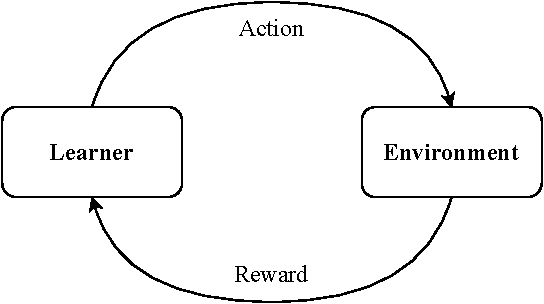
\includegraphics[width=0.33\textwidth]{Chapter0/img/mab.pdf}
    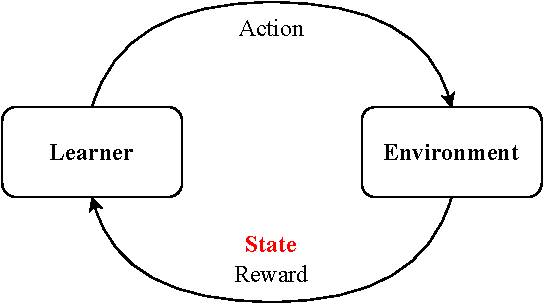
\includegraphics[width=0.33\textwidth]{Chapter0/img/rl.pdf}
    \caption{Gauche: cycle d'apprentissage bandit vs. Droite: cycle d'apprentissage RL.}
    \label{fig:abs.comparison}
\end{figure}

\section{Bandit manchot multi-bras et optimisation}\label{sec:abs.mab}
    
Cette thèse traite des problèmes d'optimisation séquentielle dans des environnements stochastiques du point de vue du bandit. Un environnement stochastique se réfère à un environnement à partir duquel des retours stochastiques sont acquis lorsqu'une entrée est demandée depuis l'espace de recherche/action\footnote{Ces termes peuvent être employés de manière interchangeable.} $\mathcal{X}$. Formellement, et sans perte de généralité, notre objectif est de maximiser une fonction cible $f:\mathcal{X}\rightarrow\mathbb{R}$, c'est-à-dire de trouver 
\begin{equation}\label{eq:abs.optim}
    \argmax_{x\in\cX} f(x)
\end{equation}
en fonction d'une séquence de valeurs de la fonction $f$. Évidemment, sans aucune information préalable sur la fonction cible et/ou l'espace de recherche $\cX$, il s'agit juste d'une mission impossible. Cette thèse étudie plusieurs instances particulières de \eqref{eq:abs.optim} avec différents espaces de recherche et/ou différentes hypothèses (de régularité) sur la fonction cible, et apporte de nouvelles perspectives théoriques et pratiques. 

Dans le reste de ce chapitre, je donne un aperçu de haut niveau des différents contextes étudiés dans cette thèse ainsi qu'un résumé de mes contributions à chaque contexte.

Une discussion plus approfondie sur la formulation du problème, en particulier sur la manière d'évaluer la performance des algorithmes dans différents contextes, est donnée dans un chapitre d'introduction~\ref{CHAP:MAB} sur le modèle de bandits. L'objectif de ce chapitre introductif est de présenter le problème de bandits de manière plus formelle. Nous rappelons d'abord quelques notions de base ainsi que certains résultats fondamentaux pour les bandits stochastiques. Nous nous concentrons ensuite sur la façon dont différents cadres d'identification du meilleur bras sont formulés.

%In its simplest form where the action space $\mathcal{X}$ is finite, the problem can be modeled as a \emph{stochastic multi-armed bandit}. The term \emph{bandit} is named, by analogy, after slot machines (or one-armed bandits) in a casino. A \emph{sequential decision making} problem comes up then when facing with several slot machines (multi-armed bandits). Concretely, a stochastic bandit is a collection of $K$ actions (also called arms) $\mathcal{X} = \{x_1,\ldots,x_K\}$. Each time the learner chooses one action $x_{a_t}\in\mathcal{X}$ which is then fed to the environment. The environment generates a reward $r_{a_t,t}=r_t$ which is assumed to be drawn from an unknown $[0,1]$-valued distribution $\nu_{a_t}$ and is revealed to the learner.

%In its original formulation, the learning objective of a stochastic bandit is to maximise the total reward $\sum_{t=1}^T r_t$ obtained within a given time horizon $T$. In the literature of bandit, we usually denote by $\mu_k$ (resp. $\mu^\star$) the expectation of the unknown distribution $\nu_k$ (resp. the optimal arm), and the previous reward maximisation objective is equivalent to minimising the \emph{cumulative regret}: $T\mu^\star-\sum_{t=1}^T \mu_{a_t}$. %A such learning objective requires the learner to simultaneously acquire new information for potential future well-being (called \emph{exploration}), and optimize the current decision based on past observations (called \emph{exploitation}). 
%Multi-armed bandits naturally addresses the trade-off between exploration and exploitation.

\subsection{Identification du meilleurs bras pour le bandit manchot multi-bras stochastique}\label{sec:abs.mab.bai}

Le premier cadre d'intérêt consiste en un espace de recherche fini et unidimensionnel $\cX = \{x_1,x_2,\cdots,x_K\}$. Supposons que la distribution de récompense sous-jacente du bras $x_k$ soit caractérisée par sa moyenne $\mu_k\in\R$, la fonction cible $f$ peut être simplement interprétée comme une correspondance entre chaque bras et sa moyenne. L'agent cherche alors à trouver
\begin{align}\label{eq:abs.optim_bai}
    \argmax_{k\in[K]} \mu_k\,
\end{align}
étant donné une certaine condition d'arrêt. Il s'agit de l'identification du meilleur bras pour les bandits multi-bras stochastiques. Il existe plusieurs objectifs d'apprentissage pour ce genre de problèmes, parmi lesquels nous sommes particulièrement intéressés par le cas où le but est d'identifier le meilleur bras avec une confiance élevée avec un minimum d'évaluations de fonctions. Il s'agit du \emph{cadre de confiance fixe} pour lequel la définition formelle, ainsi que celles pour d'autres objectifs d'apprentissage, sont fournies et discutées plus loin dans le chapitre~\ref{CHAP:MAB}.

Les méthodes existentes de ce problème nécessitent la construction d'intervalles de confiance compliqués sur les récompenses moyennes. Dans cette thèse, nous profitons des outils bayésiens pour résoudre ce problème, qui est basée sur le célèbre Thompson sampling (\citealt{thompson1933}, voir aussi~\citealt{russo2018} pour un tutoriel). Thompson sampling est un algorithme bayésien bien connu pour l'objectif classique de maximisation de la récompense, pour lequel il est maintenant considéré comme un concurrent majeur des approches populaires de type \UCB{}~\citep{auer2002ucb}. Une question naturelle à se poser est de savoir si les méthodes bayésiennes peuvent également être un bon concurrent des approches classiques de l'identification du meilleurs bras basées sur des intervalles de confiance. Cependant, il est bien connu que l'utilisation directe de Thompson sampling ne permet pas d'obtenir une performance optimale pour l'identification du meilleurs tant d'un point de vue pratique que théorique. Plus précisément, elle ne peut pas atteindre une \emph{complexité d'échantillon} asymptotique qui correspond à une borne inférieure fournie par~\cite{garivier2016tracknstop}. Une telle propriété est appelée \emph{optimalité asymptotique} dont nous donnerons une définition formelle plus tard dans le chapitre~\ref{CHAP:MAB}. Une adaptation telle que \TTTS{} proposée par~\cite{russo2016ttts} est nécessaire : en choisissant entre deux bras candidats différents à chaque tour, elle impose l'exploration de bras sous-optimaux, qui seraient sous-échantillonnés par Thompson sampling original. 

Dans le chapitre~\ref{CHAP:T3C}, nous \'etudions \TTTS{} \`a nouveau, et fournissons de nouvelles compréhensions théoriques sur sa complexité d'échantillonnage. Plus précisément, nous montrons que \TTTS{} atteint l'optimalité asymptotique qui répond alors à une question ouverte de~\cite{russo2016ttts}. Nous proposons en outre une amélioration computationnelle \TCC{} de \TTTS{}, tout en gardant les mêmes garanties. De plus, nous fournissons également de nouveaux résultats sur la convergence postérieure de \TTTS{}.

\subsection{Extension \`a l'identification du meilleurs bras lin\'eaires}\label{sec:abs.mab.linear}

Une extension du cadre pr\'ec\'edent largement étudiée consiste à prendre un ensemble fini de $K$ bras/contextes $\cX=\{\bx_1,\bx_2,\cdots,\bx_K\}\subset\R^d$ comme espace de recherche. La récompense de chaque bras dans cette circonstance est supposée linéairement d\'ependante d'un \emph{paramètre de régression} $\btheta$. La fonction cible $f$ peut donc être considérée comme une correspondance entre chaque bras $\bx$ et sa combinaison linéaire avec $\btheta$, et est donc appelée bandits linéaires. Précisément, l'agent cherche à trouver
\begin{align}\label{eq:abs.optim_linbai}
    \argmax_{k\in[K]} \btheta^\top\bx_k\,.
\end{align}
Le paramètre $\btheta$ est bien sûr \emph{inconnu} de l'agent. Ce paramètre contextuel (linéaire) décrit mieux certains scénarios du monde réel. Un exemple typique est l'optimisation du placement des publicités, dans lequel un site Web cherche à identifier le modèle d'affichage publicitaire le plus performant. Dans de telles applications, les caractéristiques des utilisateurs peuvent être utilisées comme informations secondaires (contexte) pour aider à la conception de l'exploration (voir par exemple ~\citealt{li2010contextual}).

Une fois de plus, comme pour l'identification du meilleurs bras pour les bandits stochastiques, nous nous sommes intéressés par le cadre de confiance fixe. Les algorithmes précédents sur ce sujet n'atteignent qu'une faible borne de complexité d'échantillon qui est liée à la \emph{G-optimalité} de la théorie du plan d'expérience (voir par exemple ~\citealt{pukelsheim2006optimal}). Nous conjecturons que la G-optimalité ne décrit pas au mieux la complexité de l'identification du meilleurs bras pour les bandits lin\'aires, et essayons donc d'adapter d'autres complexités plus appropriées.

Une ligne de recherche naturelle est alors de concevoir un algorithme asymptotiquement optimal. Une adaptation simple de \Track~\citep{garivier2016tracknstop} au cadre linéaire s'avère asymptotiquement optimale~\citep{jedra2020linear}, mais reste défavorable sur le plan de resources. Nous cherchons donc également à concevoir des algorithmes l\'egers en complexit\'e temporelle. 

Dans le chapitre~\ref{CHAP:LGC}, nous proposons une nouvelle complexité pour l'identification du meilleurs bras linéaire, et fournissons une comparaison complète des complexités existantes. Nous étudions ensuite \`a la fois les approches bayésiennes et les algorithmes basés sur les intervalles de confiance. En particulier, nous proposons plusieurs extensions différentes de \TTTS{} et \TCC{} au cadre linéaire. Malheureusement, nous montrons empiriquement qu'elles ne sont pas asymptotiquement optimales. Dans le même temps, nous développons une approche utilisant le point de selle qui conduit à un algorithme optimal \LG{}.

\subsection{Bandits infinis et optimisation bo\^ite noire}\label{sec:abs.mab.bbo}

Enfin, un problème plus général consiste à considérer un espace infini ou continu $\cX$, et chaque bras $x\in\mathcal{X}$ obtient sa récompense moyenne $f(x)$ par la fonction de récompense $f$. On retrouve donc~\eqref{eq:abs.optim} :
\[
    \argmax_{x\in\cX} f(x)\,.
\]
Il s'agit du problème de l'optimisation globale ou optimisation bo\^ite noire. Parfois, nous pouvons également parler de l'optimisation du zero ordre, par opposition à \emph{optimisation du premier ordre} pour lequel des informations basées sur le gradient sont disponibles.

Nous étudions le cas stochastique dans cette thèse. Les approches typiques pour traiter l'optimisation globale incluent l'optimisation bay\'esienne (voir par exemple ~\citealt{brochu2010bayesian}), les algorithmes évolutionnaires et les bandits hiérarchiques (voir par exemple ~\citealt{bubeck2010x}). Dans cette thèse, nous nous concentrons sur les algorithmes de bandits hiérarchiques. Dans la littérature, nous faisons souvent référence aux \emph{bandits à bras infinis} ou bien aux \emph{bandits à bras continus}.

De toute évidence, on ne peut s'attendre qu'à une solution \emph{quasi-optimale} dans le cas des bandits à bras continus. Nous utilisons donc une autre mesure de performance, à savoir le \emph{regret simple}, qui est la différence entre la valeur de la fonction optimale réelle et la valeur de la fonction de notre estimation finale. La définition formelle est fournie plus loin dans le chapitre~\ref{CHAP:MAB}.
Le regret simple diffère du \emph{regret cumul\'e} qui sert de mesure de performance pour la maximisation de la récompense. 

Dans le chapitre~\ref{CHAP:GPO}, nous explorons la possibilité de concevoir des algorithmes de bandit hiérarchique sans paramètre avec un minimum d'hypothèses. À cette fin, nous utilisons une astuce de validation croisée et construisons un algorithme appelé \GPO{}. \GPO{} est un méta-algorithme qui peut utiliser n'importe quel algorithme de bandit hiérarchique comme sous-routine. En particulier, \GPO{} atteint presque la même garantie de regret simple que sa sous-routine. Comme résultat secondaire, nous montrons également que \HCT{} est un algorithme sous-jacent valide pour \GPO{} ainsi que pour \POO{} proposé par~\cite{grill2015poo}. 

%In a recent work of ours, we provide a general wrapper for hierarchical bandit algorithms that only have guarantees for their simple regret~\cite{shang2019adaptive}. We show that with a cross-validation scheme, any hierarchical bandit algorithm with simple regret guarantees can be plugged into our meta-algorithm with only a tiny increase in the resulting simple regret.

\subsection{Optimisation des hyper-param\`etres}\label{sec:abs.mab.hpo}

Enfin, nous abordons une question plus pratique : l'optimisation des hyper-paramètres. Comme présenté dans la section~\ref{sec:abs.context.what}, le réglage efficace des hyper-paramètres pourrait être d'une grande importance pour les praticiens de l'apprentissage automatique. Comme indiqué, l'optimisation des hyper-paramètres peut être naturellement modélisé comme un problème d'optimisation séquentielle. L'espace de recherche dans ce cadre peut être à la fois discret (variables catégoriques, variables à valeur entière, etc.) et continu (variables à valeur réelle). 

%Il est naturel de se demander si les algorithmes de bandit hiérarchique sont capables d'atteindre des performances compétitives par rapport aux algorithmes classiques bas\'es sur l'optimisation bay\'esienne.

Inspirés par un algorithme récent \Hyperband{} basé sur l'identification du meilleurs bras~\citep{li2017hyperband}, nous cherchons à proposer d'autres algorithmes pour l'optimisation des hyper-paramètres aussi basés l\`a-dessus. En effet, \Hyperband{} est construit sur un algorithme basé sur l'élimination et a de bonnes performances par rapport aux méthodes précédentes. D'autre part, nous nous intéressons à la possibilité d'adapter des algorithmes bayésiens tels que \TTTS{} pour résoudre l'optimisation des hyper-paramètres. Notez que \TTTS{} n'est conçu que pour les \emph{bandits à bras finis}, un contournement appropriée est donc nécessaire.

Dans le chapitre~\ref{CHAP:DTTTS}, nous concevons un algorithme robuste et dynamique \DTTTS{} basé sur \TTTS{}, et montrons que de tels algorithmes à saveur bayésienne peuvent être de bons candidats pour des applications comme l'optimisation des hyper-paramètres. Nous discutons également d'un inconvénient majeur de \DTTTS{}, et proposons une solution dans le même chapitre.

    %\chapter*{Acknowledgement}




	\cleardoublepage
		% Table des matières
		\setcounter{tocdepth}{1}	% Pas besoin de trop détailler le sommaire ici (chapitres/sections)
		\dominitoc						% Génération des mini-toc	\pagenumbering{arabic}
		\tableofcontents
		% Liste des algos
		\clearpage
        \addcontentsline{toc}{chapter}{List of Algorithms}
        \listofalgorithms
		% Liste des figures
		\renewcommand*\listfigurename{List of Figures}
		\listoffigures
		% Liste des tableaux
		\listoftables
		

%%%%%%%%%%%%%%%%%%%%%%%%%%%%%%%%%%%%%
%        Contenu du document        %
%%%%%%%%%%%%%%%%%%%%%%%%%%%%%%%%%%%%%
	\setcounter{mtc}{4}	% "Corrige" les minitocs décallés à cause des chapter* (ex : table des matières)
	\pagenumbering{arabic}
	%%%%%%%%%%%%%%%%%%%%%%%%%%%%%%%%%%%%%%%%%%%%%%%%%%%%%%%%%%%%%%%%%%%%%%%%%%%%%%%%%%%%%%%%%%%%%
%%									Chapitre 1											%
%%%%%%%%%%%%%%%%%%%%%%%%%%%%%%%%%%%%%%%%%%%%%%%%%%%%%%%%%%%%%%%%%%%%%%%%%%%%%%%%%%%%%%%%%%%%%
\chapter{An Overview of the Thesis}\label{chap:intro}
	\citationChap{
	The thing about quotes on the internet is that you can not confirm their validity
	}{Abraham Lincoln}
	\minitoc
	\newpage

%%%%%%%%%%%%%%%%%%%%%%%%%%%%%%%%%%%%%%%%%%%%%%%%%%%%%%%%%%%%%%%%%%%%%%%%%%%%%%%%%%%%%%%%%%%%%



% Début du chapitre

The purpose of this thesis is to provide a summary of the main research line of my PhD work carried out in between October 2017 and March 2021. During my PhD, I was hosted at the Inria Lille-Nord Europe (France) research center, in the SequeL team (now becomes Scool team). I was fortunate to be advised by Dr. Michal Valko, and also co-supervised by Dr. Emilie Kaufmann. The research thematic of SequeL lies in sequential decision making problems, to which all my contributions are devoted. In particular, this document mainly investigates sequential decision making in optimization problems.

\section{Context of the Thesis}\label{sec:intro.context}
	
\subsection{What do we study and why?}\label{sec:intro.context.what}

Imagine that we dispose a simulator for some complex numerical task. Being considered as a black box, we can only get useful information by calling the simulator with different inputs. The goal is to find an input that optimizes the performance of the simulator. In the context of this thesis, we model such a scene as the so-called \gls{sequential optimization}\footnote{We thus do not consider parallelization in this thesis.} problem where a learner sequentially feeds inputs to an environment (the simulator in the previous example) and from which they receive (deterministic or stochastic) feedback/payoffs/rewards/observations\footnote{Those terms can be interchangeably employed.}. After a certain period of trial, the learner shall be able to output a guess for the optimal input. Under some circumstances, a single interaction with the environment could be extremely costly. It is therefore of great interest to carefully choose the input at each time step based on past observations.

Sequential optimization in a stochastic environment is an active research topic in both applied mathematics and computer science communities. For example, the planning problem in a \gls{mdp}, upon which the recent breakthrough of game intelligence of Go~\citep{silver2016alphago} is constructed, is closely related to sequential optimization. Precisely, given the current state of the game, the game intelligence is designed to maximize a certain value function, whose (noisy) observations can be obtained by exploring well-chosen trajectories.

Another example, which is also one important driving force that motivates this thesis originally, is \gls{hpo} of machine learning classifiers. Modern machine learning algorithms often contain many nuisance parameters that cannot be learned through the learning process, but instead, need to be manually specified. Tuning those so-called \gls{hyper-parameters} is often considered as the most tedious part in a data science task. It is hence appealing to design HPO algorithms that automates the process of choosing those hyper-parameters. HPO can be viewed as a BBO problem where function evaluations are supposed to be very expensive. Typically, a function evaluation in HPO involves running the primary machine learning algorithm to completion on a large and high-dimensional dataset, which often takes a considerable amount of time or resources.

Besides, sequential optimization can also serve as an abstraction of numerous real-world problems. To name a few of them, we can think of (risk-averse) portfolio selection problems in finance~\citep{ziemba2010}, designing effective treatment allocation strategies in medicine~\citep{durand2018contextual}, free-energy minimization in chemical engineering or protein structure prediction~\citep{floudas2000}, metamodelling for engineering design optimization~\citep{wang2007}, parameter estimation (inverse problem) of nonlinear dynamic biochemical pathways~\citep{moles2003}, mesh distortion in material science~\citep{charpagne2019ebsd}, and way more. 

Mathematically speaking, an environment is simply a target function to be optimized. This function can be \textbf{discrete or continuous}. In this thesis, we are in particular interested in optimization of functions for which \textbf{none (or few)} regularity assumptions are made, and only \textbf{noisy (or stochastic)} function evaluations (interactions with the environment) can be observed.

%Le problème de planification dans un Processus de Décision Markovien (MDP pour Markov Decision Process, [1]), pouvant modéliser la gestion de ressources dans un système de type smart grids ou encore le contrôle d'un robot, et celui de la construction d'intelligences artificielles pour des jeux, sont très liés à celui de l'optimisation séquentielle puisqu'ils reviennent à déterminer l'action qui dans un état donné maximise une fonction valeur, dont on peut obtenir des réalisations bruitées en explorant des trajectoires bien choisies.

%In this context, since one does not make extra regularity assumptions on the target function, one can imagine that it can be very costly to evaluate the function. Thus a good strategy for choosing adaptively the next observation is needed in order to find an optimal (or quasi-optimal) point with as few number of evaluations as possible. This is the sequential optimization problem. That being said, the main problematic of my thesis is the \emph{global sequential optimization} problem. Several applications could be investigated in this thesis, in particular the \emph{automatic hyper-parameter tuning} of machine learning algorithms~\citep{samothrakis2013,hoffman2014bayesgap,jamieson2016hyperband,li2017hyperband}.

\subsection{How do we approach the problem?}\label{sec:intro.context.how}

Sequential optimization problem has been widely inspired by the literature of~\gls{mab}. The original MAB problem is first studied by~\cite{thompson1933}, and can be described in the following way: A learner is given a \emph{finite} set of $K$ arms and a time horizon $T$. Pulling an arm leads to a stochastic reward that follows some \emph{unknown} distribution underpin that arm. At each time step, the learner can choose to pull one of the arms and observes a reward sampled from its corresponding underlying distribution.

% \begin{remark}\label{remark:partial}
% \begin{leftbar}[remarkbar]
% Note that rewards of unchosen arms at each time step are not revealed: this partially observable feedback setting is thus a special case of the online learning with experts setting.
% \end{leftbar}
% \end{remark}

In its original form, the objective of a MAB learner is to maximize the total rewards in the long run. A natural observation is that, the learner is required to simultaneously acquire new information for potential future well-being (exploration), and optimize the current decision based on past observations (exploitation). Such phenomena is stated as the \gls{exploration-exploitation dilemma}, and is present in many real-world tasks. The MAB model is thus popular among different communities as it trades off exploration and exploitation naturally.
%The usual performance criterion of the learner is measured by the total loss of the chosen arm at each time step w.r.t the best arm, namely the \emph{cumulative regret}. Typical good learners like \UCB~\citep{auer2002ucb} trade off between exploration and exploitation. 

However, exploitation does not necessarily provide meaningful incentives in some real applications. Typically, in the previous working examples presented in Section~\ref{sec:intro.context.what}, we do not really care about the potential losses incurred during the whole learning phase. Indeed, we only aim at finding the (near-)optimum of the target function quickly. In this context, it is more natural to assess the learner in an optimization fashion. This setting, often named as \gls{bai}, is thus more closely related to what we are to investigate in this thesis.

\begin{remark}
\begin{leftbar}[remarkbar]
More generally, we talk about \gls{pure exploration} problems~\citep{bubeck2011pure} instead of BAI, where the learner is supposed to gain as much information about the bandit model regardless of rewards. BAI is merely a particular instance of pure exploration, for which the learning objective is to find the optimal arm. Other learning objectives also exist, like finding arms that surpass some pre-defined threshold (see e.g.~\citealt{locatelli2016thresholding}). However, we mostly focus on BAI in this thesis since it is sufficiently representative.
\end{leftbar}
\end{remark}

\subsection{From multi-armed bandits to reinforcement learning}\label{sec:intro.context.rl}

The MAB model is popular from another perspective as it is part of the more general \gls{rl} framework. In RL, a learner is characterized by its current state and interacts with the environment by taking different actions. Each action leads to a reward from the environment as well as a change of states. Formal definition and general results of RL are beyond the scope of this thesis, lecturers can refer to~\cite{sutton1998,bertsekas2011approximate} for surveys. 

Modern RL combined with \gls{dl} has marked a handful of exciting breakthroughs including AlphaGo~\citep{silver2016alphago}, AlphaStar, AlphaFold, etc. However, a big gap still exists in understanding the huge success of Deep RL. MAB, as a strongly theoretically-grounded statistical model, can potentially serve as a first step towards filling that gap in RL research. More precisely, MAB is sometimes considered as the simplest form of RL as MAB learners do not incur any change of states (see Fig.~\ref{fig:intro.comparison}). We shall discuss a little more the link between MAB and RL later in the general conclusion Chapter~\ref{chap:conclusion} as contextual MAB (MAB with side information) -- a variant of the vanilla MAB model -- describes eventually better how MAB is related to RL.

\begin{figure}[ht]
    \centering
    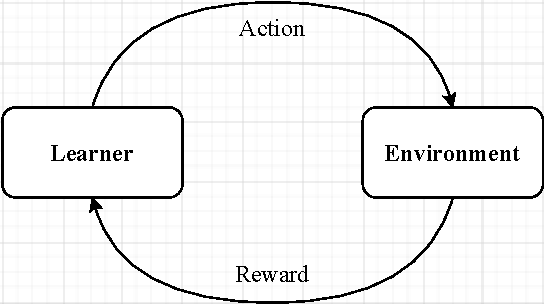
\includegraphics[width=0.33\textwidth]{Chapter1/img/mab.pdf}
    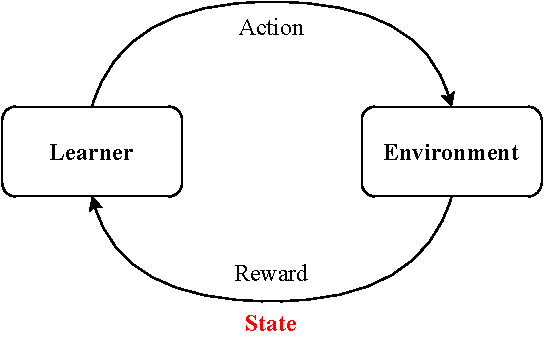
\includegraphics[width=0.33\textwidth]{Chapter1/img/rl.pdf}
    \caption{Left: a bandit learning cycle vs. Right: a reinforcement learning cycle.}
    \label{fig:intro.comparison}
\end{figure}

\section{Multi-Armed Bandits and Optimization}\label{sec:intro.mab}
    
This thesis tries to address sequential optimization problems under stochastic environments from a bandit point of view. A stochastic environment refers to an environment from which stochastic feedback are acquired when an input is queried from the search/action space\footnote{Those terms can be interchangeably employed.} $\mathcal{X}$. Formally, and without loss of generality, we aim to maximize\footnote{Minimization is obviously the same problem.} a target function $f:\mathcal{X}\rightarrow\mathbb{R}$, i.e. find 
\begin{equation}\label{eq:optim}
    \argmax_{x\in\cX} f(x)
\end{equation}
based on a sequence of function values of $f$. Obviously without any prior information on the target function and/or the search space $\cX$, it is just a find-a-needle-in-a-haystack mission. This thesis studies several particular instances of \eqref{eq:optim} with various search spaces and/or different (regularity) assumptions on the target function though, and brings both novel theoretical and practical insights. 

Before jumping into details, we provide a brief overview of different settings investigated in this thesis in this section. More thorough discussion on the problem formulation, in particular how do we assess the performance of algorithms under different settings is given in Chapter~\ref{chap:mab}.

%In its simplest form where the action space $\mathcal{X}$ is finite, the problem can be modeled as a \emph{stochastic multi-armed bandit}. The term \emph{bandit} is named, by analogy, after slot machines (or one-armed bandits) in a casino. A \emph{sequential decision making} problem comes up then when facing with several slot machines (multi-armed bandits). Concretely, a stochastic bandit is a collection of $K$ actions (also called arms) $\mathcal{X} = \{x_1,\ldots,x_K\}$. Each time the learner chooses one action $x_{a_t}\in\mathcal{X}$ which is then fed to the environment. The environment generates a reward $r_{a_t,t}=r_t$ which is assumed to be drawn from an unknown $[0,1]$-valued distribution $\nu_{a_t}$ and is revealed to the learner.

%In its original formulation, the learning objective of a stochastic bandit is to maximise the total reward $\sum_{t=1}^T r_t$ obtained within a given time horizon $T$. In the literature of bandit, we usually denote by $\mu_k$ (resp. $\mu^\star$) the expectation of the unknown distribution $\nu_k$ (resp. the optimal arm), and the previous reward maximisation objective is equivalent to minimising the \emph{cumulative regret}: $T\mu^\star-\sum_{t=1}^T \mu_{a_t}$. %A such learning objective requires the learner to simultaneously acquire new information for potential future well-being (called \emph{exploration}), and optimize the current decision based on past observations (called \emph{exploitation}). 
%Multi-armed bandits naturally addresses the trade-off between exploration and exploitation.

\subsection{Best-arm identification for stochastic multi-armed bandits}\label{sec:intro.mab.bai}

The first setting of interest consists of a finite and one-dimensional search space $\mathcal{X} = \{x_1,x_2,\cdots,x_K\}$. Assume that the underlying reward distribution of arm $x_k$ is characterized by its mean $\mu_k\in\R$, the target function $f$ can be simply interpreted as a mapping form each arm to its mean. The learner then aims to find
\begin{align}\label{eq:optim_bai}
    \argmax_{k\in[K]} \mu_k\,
\end{align}
given some stopping condition. This is the best-arm identification for stochastic multi-armed bandits. Several learning objectives exist for a general BAI problem, among which we are in particular interested in the setting of which the goal is to identify the best arm with high confidence based on a minimum of function evaluations. This is the \gls{fixed-confidence setting} for whom the formal definition, along with those for other learning objectives, are provided and discussed later in Chapter~\ref{chap:mab}.

Existing methods for BAI for stochastic MAB often requires construction of complicated confidence intervals of the mean estimates. We opt for Bayesian machinery to address this problem in this thesis, which is based on the famous Thompson sampling (\TS). \TS is a Bayesian algorithm well known for the classical reward maximization objective, for which it is now seen as a major competitor to the popular \UCB-typed approaches~\citep{auer2002ucb}. A natural question to ask is whether Bayesian methods can be also a good competitor to classical BAI approaches constructed upon complicated confidence intervals. However, it is well known that straight application of \TS cannot yield optimal performance for BAI both in a practical and theoretical point of view. More precisely, it cannot achieve an asymptotic \gls{sample complexity} that matches the lower bound provided by~\cite{garivier2016tracknstop}. Such property is called \gls{asymptotic optimality} that we shall give formal definition later in Chapter~\ref{chap:mab}. An adaptation such as \TTTS proposed by~\cite{russo2016ttts} is needed: by choosing between two different candidate arms in each round, it enforces the exploration of sub-optimal arms, which would be under-sampled by vanilla \TS due to its objective of maximizing rewards. 

In this thesis, we revisit \TTTS both in theory and in practice, trying to provide new insights on its convergence and complexity, and also improve its computational performance.

\subsection{Extension to best-arm identification for linear bandits}\label{sec:intro.mab.linear}

Beyond the previous vanilla setting of BAI, a very natural and widely studied extension is to take a finite set of $K$ arms/contexts/features\footnote{Those terms can be interchangeably employed in the context of this thesis.} $\cX=\{\bx_1,\bx_2,\cdots,\bx_K\}\subset\R^d$ as the search space. The reward of each arm under this circumstance is assumed to depend linearly on a \gls{regression parameter} $\btheta$. The target function $f$ therefore can be considered as a mapping from each arm $\bx$ to its linear combination with $\btheta$, and is thus called linear bandits. Precisely, the learner seeks to find
\begin{align}\label{eq:optim_linbai}
    \argmax_{k\in[K]} \btheta^\top\bx_k\,.
\end{align}
The parameter $\btheta$ is of course \emph{unknown} to the learner. This linear contextual setting describes better some real-world scenarios like advertising placement optimization, and therefore often attracts great attention.

Again, we are interested in the fixed-confidence setting. Previous algorithms on this topic only achieve loose sample complexity bound which is linked to the \gls{G-optimality} of experimental design theory (see e.g.~\citealt{pukelsheim2006optimal}). We conjecture that G-optimality does not describe best the complexity of linear bandits BAI, and therefore try to opt for other more appropriate complexities.

One natural research line is then to design asymptotically optimal algorithm. A simple adaptation of \Track~\citep{garivier2016tracknstop} to the linear setting is very likely to be asymptotically optimal, but remains computationally unfavorable. We thus also seek to design computational friendly algorithms. In this thesis, we investigate both Bayesian approach and confidence interval-based algorithms. In particular, we study whether extensions of \TTTS can be asymptotically optimal.
%Unfortunately, they do not seem to be (asymptotically) optimal (work not published yet). Therefore, knowing whether one can find an *optimal* Bayesian approach remains an open problem.

\subsection{Infinitely-armed bandits and black-box optimization}\label{sec:intro.mab.bbo}

Finally, a more general problem is to consider an infinite (probably uncountable) measurable space $\mathcal{X}$, and each arm $x\in\mathcal{X}$ gets its mean reward $f(x)$ through the reward function $f$. We thus recover~\eqref{eq:optim}:
\[
    \argmax_{x\in\cX} f(x)\,.
\]
This is the \gls{go} or \gls{bbo} problem. Sometimes we can also refer to \gls{zo}, in contrast to \emph{first-order optimization} for which gradient-based information is available.

We study the noisy setting in this thesis. Typical approaches to address GO include \gls{bo} (see e.g.~\citealt{brochu2010bayesian}), evolutionary algorithms and hierarchical bandits (see e.g.~\citealt{bubeck2010x}). In this thesis, we focus on hierarchical bandits algorithms. In the literature of bandits, we often refer to \gls{infinitely-armed bandits} or more precisely \gls{continuum-armed bandits}.

Obviously, we can only expect for a \emph{near-optimal} solution under continuum-armed bandits. We thus opt for another performance measure, namely the \gls{simple regret}, which is the difference between the true optimal function value and the function value of our final guess. Simple regret differs from \gls{cumulative regret} which serves as the performance measure for reward maximization. Formal definitions are provided later in Chapter~\ref{chap:mab}.

In this thesis, we explore the possibility of designing parameter-free hierarchical-bandit algorithms with minimum (smoothness) assumptions.

%In a recent work of ours, we provide a general wrapper for hierarchical bandit algorithms that only have guarantees for their simple regret~\cite{shang2019adaptive}. We show that with a cross-validation scheme, any hierarchical bandit algorithm with simple regret guarantees can be plugged into our meta-algorithm with only a tiny increase in the resulting simple regret.

\subsection{Hyper-parameter optimization}\label{sec:intro.mab.hpo}

Finally, we turn our attention to a more practical question: hyper-parameter optimization. As introduced in Section~\ref{sec:intro.context.what}, efficient hyper-parameter tuning could be of great importance for machine learning practitioners. As is stated, HPO can be naturally modelled as a sequential optimization problem.

The search space of HPO can be both discrete (categorical variables, integer-valued variables, etc) and continuous (real-valued variables). It is natural to ask if hierarchical-bandit algorithms are able to achieve competitive performances for HPO against classical BO algorithms.

Additionally, inspired by a recent BAI-based algorithm \Hyperband~\citep{li2017hyperband}, we seek to propose other BAI-based algorithms for HPO. Indeed, \Hyperband is constructed upon an elimination-based BAI algorithm and achieves state-of-the-art performances compared to previous methods. We, on the other hand, are interested in whether Bayesian algorithms like \TTTS can also be adapted to tackle HPO problems. Note that \TTTS is only designed for \gls{finitely-armed bandits}, an appropriate workaround is hence needed.

\section{A Summary of the PhD}\label{sec:intro.contributions}

From Section~\ref{sec:intro.mab} we can see that the entire thesis is dedicated to one single problem -- sequential bandit optimization -- only with different settings. The full journey of my PhD is, however, far beyond the scope of the present manuscript. This thesis is by no means intended to introduce all the results I have obtained, but rather tell a story about the bandit optimization research line. 

The purpose of this section is to provide a summary of the contributions included in this thesis, and also list all the other work I have participated to just for the record.

\subsection{Summary of the contributions in this thesis}\label{sec:intro.contributions.summary}

We can summarize the contributions presented in this thesis as listed below.

\begin{itemize}[label=\ding{43}]
    \item \cite{shang2020t3c} revisits a Bayesian BAI algorithm \TTTS, and provides new theoretical understandings on its posterior convergence.
    \item \cite{shang2020t3c} also shows that \TTTS achieves asymptotic optimality on the sample complexity.
    \item \cite{shang2020t3c} further proposes a computational improvement \TCC of \TTTS, whilst keeping the same guarantees.
    \item \cite{degenne2020game} proposes a new linear bandits BAI complexity, and provides a comprehensive comparison of existing complexities.
    \item In an unpublished work, we propose several different extensions of \TTTS and \TCC to the linear setting. Unfortunately, we show empirically that they are not asymptotically optimal. In the meantime, \cite{degenne2020game} develops a saddle-point approach that leads to optimal algorithms \LG and \LGC.
    \item \cite{shang2019adaptive} proposes a general wrapper \GPO, using a cross-validation scheme, that wraps up all hierarchical bandit algorithms with simple regret guarantees.
    \item \cite{shang2018adaptive} shows that \HCT is a valid underlying algorithm for \GPO as well as \POO by~\cite{grill2015poo}.
    \item \cite{shang2019dttts} designs a robust and dynamic algorithm \DTTTS based on \TTTS, and shows that such Bayesian-flavored algorithms can be good candidates for applications like hyper-parameter optimization.
    \item \cite{shang2020dttts} provides some further understandings of \DTTTS.
\end{itemize}

\subsection{List of publications and other work}\label{sec:intro.contributions.list}

\paragraph{List of papers (peer-reviewed publications or preprints) included in this thesis.}

\begin{itemize}[label=\ding{171}]
    \item Gamification of pure exploration for linear bandits. In Proceedings of the 37th International Conference on Machine Learning (ICML), 2020.~\citep{degenne2020game}
    \item Fixed-confidence guarantees for Bayesian best-arm identification. In Proceedings of the 23rd International Conference on Artificial Intelligence and Statistics (AIStats), 2020.\citep{shang2020t3c}
    \item Simple (dynamic) bandit algorithms for hyper-parameter optimization. Preprint, 2020.~\citep{shang2020dttts}
    \item A simple dynamic bandit algorithm for hyper-parameter tuning. In 6th Workshop on Automated Machine Learning at International Conference on Machine Learning (ICML-AutoML), 2019.~\citep{shang2019dttts}
    \item General parallel optimisation without a metric. In Proceedings of the 30th International Conference on Algorithmic Learning Theory (ALT), 2019.~\citep{shang2019adaptive}
    \item Adaptive black-box optimisation got easier: HCT needs only local smoothness. In 14th European Workshop on Reinforcement Learning (EWRL), 2018.~\citep{shang2018adaptive}
    \item Hierarchical bandits for black-box optimization and Monte-Carlo tree search. Master Thesis, 2017.~\citep{shang2017master}
\end{itemize}

\paragraph{List of papers (peer-reviewed publications or preprints) not included in this thesis.}

The list below presents other work that are not included in this thesis since they do not really fit in with the scope of the main story line.

\begin{itemize}[label=\ding{171}]
    \item Safe best-arm-identification in linear bandits. Preprint, 2021.~\citep{shang2021safe}
    \item UCB momentum Q-learning: Correcting bias without forgetting. In Proceedings of the 38th International Conference on Machine Learning (ICML), 2021.~\citep{menard2021ucbmq}
    \item Stochastic bandits with vector losses: Minimizing infinite norm of relative losses. Preprint, 2020.~\citep{shang2020vector}
\end{itemize}

\paragraph{Open source software.}

\begin{itemize}[label=\ding{171}]
    \item rlberry - A reinforcement learning library for research and education. Github Repository, 2021.~\citep{rlberry2021}
\end{itemize}

\section{Organization of the Thesis}\label{sec:intro.organization}

We conclude this chapter by providing an outline of the main text of the thesis. 

We start by an introductory Chapter~\ref{chap:mab} about the MAB model. The purpose of this chapter is to present the MAB problem in a more formal way. We first recall some basic notions as well as some fundamental results for stochastic MAB. We then focus on how different best-arm identification/global optimization settings previously mentioned in Section~\ref{sec:intro.mab} are formulated from a bandit point of view.

Chapter~\ref{chap:t3c} is dedicated to the problem of stochastic best-arm identification, where we study in particular Bayesian approaches. This chapter is based on the results presented by~\cite{shang2020t3c}.

Chapter~\ref{chap:lgc} studies best-arm identification for linear bandits. We first investigate the problem from a Bayesian point of view based on some unpublished work. Besides, we also present some general results of linear bandits BAI~\citep{degenne2020game}. 

Chapter~\ref{chap:gpo} is dedicated to continuum-armed bandits. This chapter is mainly based on the results presented by~\cite{shang2018adaptive} and~\cite{shang2019adaptive}.

We talk about one important application of previous problem settings in Chapter~\ref{chap:dttts}, namely \gls{automated machine learning}. We focus especially on hyper-parameter optimization. This chapter is partly based on the results by~\cite{shang2019dttts,shang2020dttts}, but also includes some discussion from my master thesis~\cite{shang2017master}.

Finally, we conclude the present manuscript by some general discussions as well as some future perspectives in Chapter~\ref{chap:conclusion}.

% \newpage
% \bibliographystyle{plain}
% \bibliography{library}

	%%%%%%%%%%%%%%%%%%%%%%%%%%%%%%%%%%%%%%%%%%%%%%%%%%%%%%%%%%%%%%%%%%%%%%%%%%%%%%%%%%%%%%%%%%%%%%
%%									Chapitre 2											%
%%%%%%%%%%%%%%%%%%%%%%%%%%%%%%%%%%%%%%%%%%%%%%%%%%%%%%%%%%%%%%%%%%%%%%%%%%%%%%%%%%%%%%%%%%%%%
\chapter{Stochastic Multi-Armed Bandits}\label{chap:mab}
	\citationChap{
	blabla
	}{}
	\minitoc
	\newpage

%%%%%%%%%%%%%%%%%%%%%%%%%%%%%%%%%%%%%%%%%%%%%%%%%%%%%%%%%%%%%%%%%%%%%%%%%%%%%%%%%%%%%%%%%%%%%

\section{The Multi-Armed Bandits Model}\label{sec:mab.model}

The problem of sequentially allocating resources to a defined set of actions (arms) based on successive \emph{partially observable} (see Definition~\ref{def:mab.mab} and Remark~\ref{remark:mab.partial} below) feedback refers to the MAB problem in probability theory. The term \emph{bandit} is named, by analogy, after slot machines (or one-armed bandits) in a casino. A sequential decision making problem comes up then when facing with several slot machines (multi-armed bandits).

The study of MAB problems can date back to as early as 1933~\citep{thompson1933}, and was originally proposed to model sequential clinical trials. For example, researchers testing the efficacy of potential vaccines for a new coronavirus have to choose a vaccine (arm) from the following 4 options as shown in Fig.~\ref{fig:mab.covid} on each patient from an experimental group of $T$ person. For each patient $t\in[T]$, researchers receive a reward signal $r_t\in\{0,1\}$. $r_t=1$ indicates that the treatment is successful, otherwise the treatment is a failure. We thus assume that the efficacy of each vaccine follows some Bernoulli distribution that is unknown to the researchers.

\begin{figure}[ht]
    \centering
    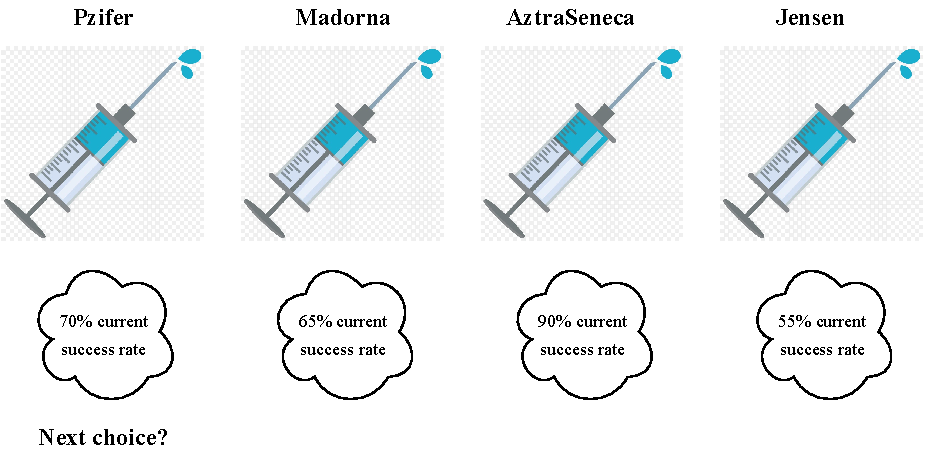
\includegraphics[width=\textwidth]{Chapter2/img/covid.pdf}
    \caption{An example of modelling clinical trials as a MAB problem.}
    \label{fig:mab.covid}
\end{figure}

As stated in Chapter~\ref{chap:intro}, a common learning objective for stochastic MAB is to maximize the total reward obtained given a sequence of observations. In the previous example, researchers need to decide which vaccine to employ for each patient depending on the previous success rates with the purpose of maximizing the total success rate $\sum_{t=1}^T r_t$ at the end.

In this section, we go beyond the intuition and provide the formal definition of the model. We also recall some fundamental results for the sake of self-containedness. Of course, we do not intend to write a survey of MAB, for which the content is far too rich for this thesis. Interested lecturers can refer to~\cite{bubeck2012bandits,lattimore2018bandits} or~\cite{slivkins2019bandits} for further readings and more recent results.

\subsection{Problem Formulation}\label{sec:mab.model.formulation}

Recall that a bandit learning cycle can be described as in Fig.~\ref{fig:mab.mab}. An MAB problem can be formulated as follow.

\begin{figure}[ht]
    \centering
    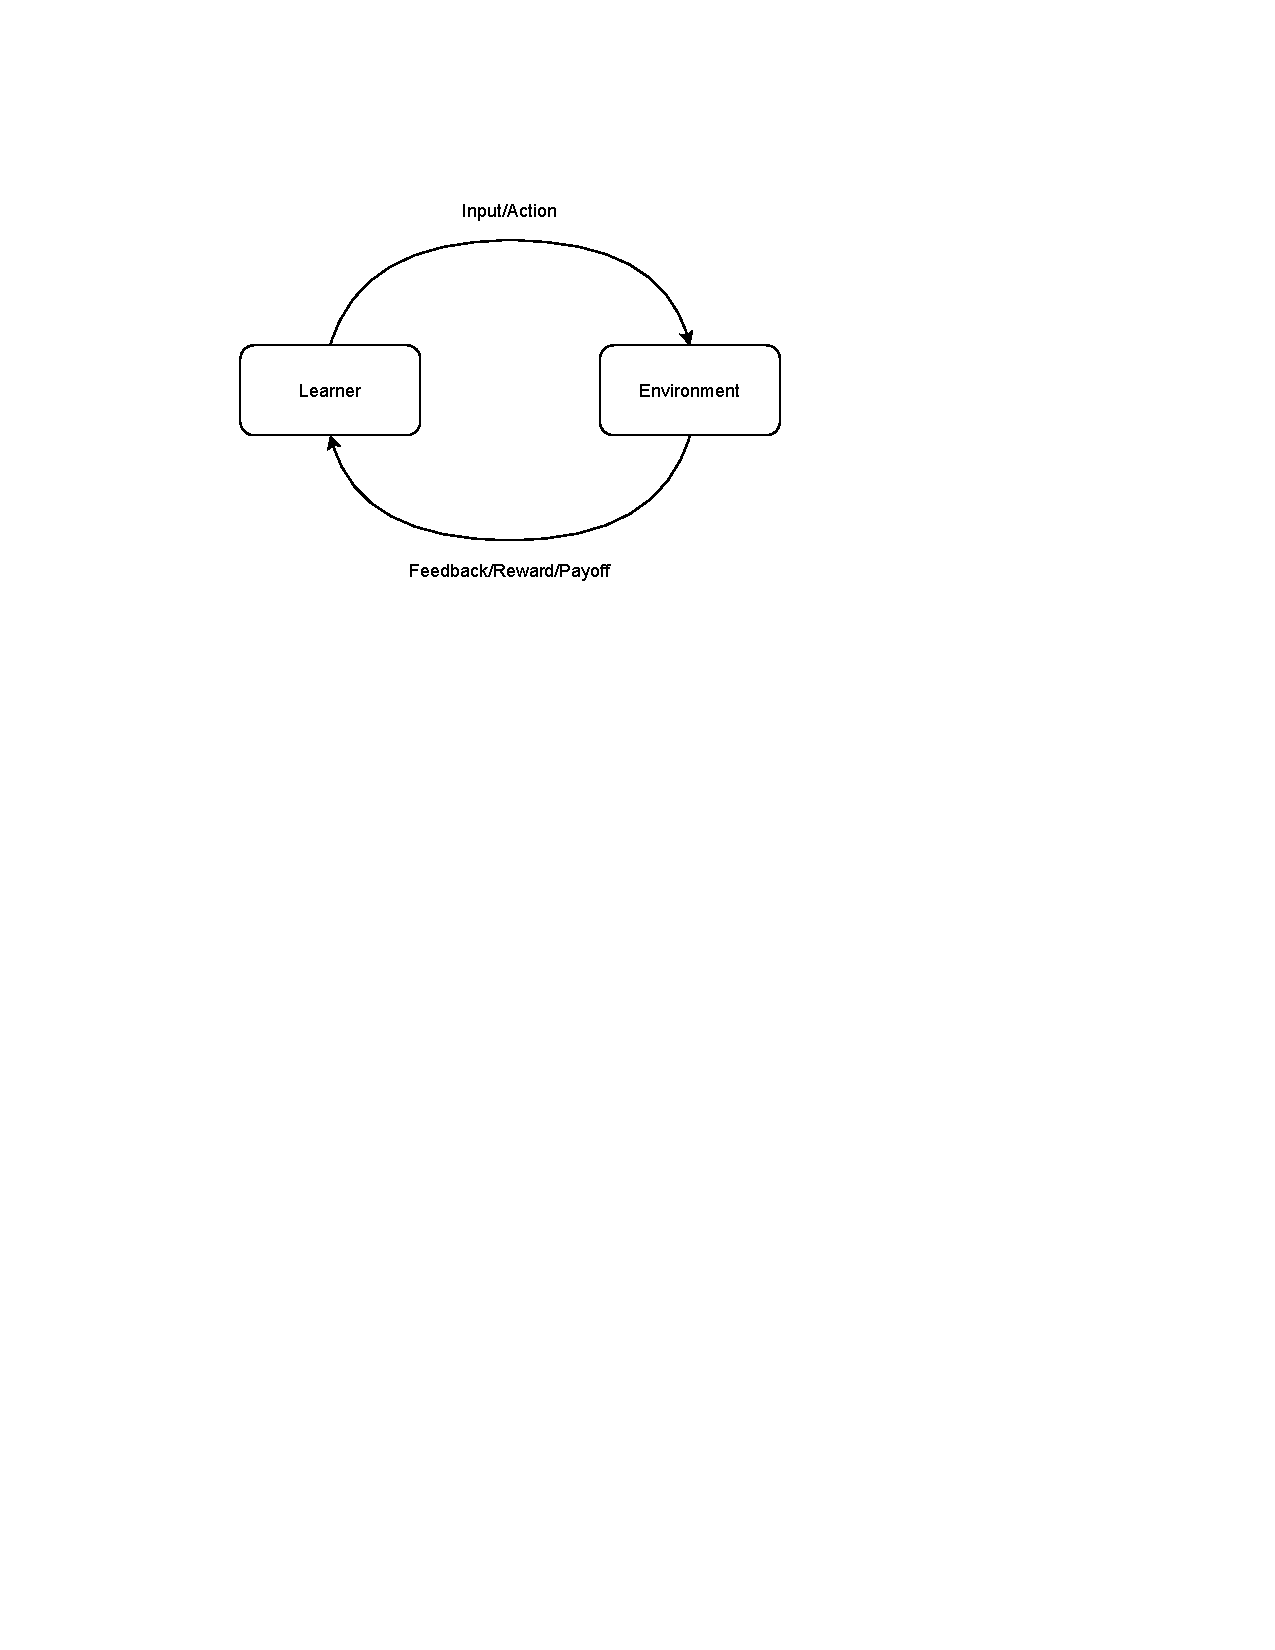
\includegraphics[width=0.5\textwidth]{Chapter2/img/mab.pdf}
    \caption{A bandit learning cycle.}
    \label{fig:mab.mab}
\end{figure}

\begin{definition}[multi-armed bandit problem]\label{def:mab.mab}
\begin{leftbar}[defnbar]
	We are given a set of $K$ arms $\{1,\ldots,K\}$ that follow $K$ unknown $[0,1]$-valued distributions $(\nu_k)_{1 \leq k \leq K}$, and a time horizon $T$. At each time step $t$, the process consists of the following actions:
	\begin{itemize}
		\item a vector of rewards $(r_{1,t} \sim \nu_1, \ldots, r_{K,t} \sim \nu_K)$ is generated,
		\item the learner picks an arm $k_t \in \{1,\ldots,K\}$, and
		\item the learner observes the reward $r_t = r_{k_t, t}$.
	\end{itemize}
\end{leftbar}
\end{definition}

\begin{remark}\label{remark:mab.partial}
\begin{leftbar}[remarkbar]
	Rewards of unchosen arms at time $t$ are not revealed, this partial feedback setting is a special case of the online learning with experts setting.
\end{leftbar}
\end{remark}

\subsection{Regret minimization}\label{sec:mab.model.regret}

As we have mentioned in Chapter~\ref{chap:intro} that one needs to trade-off between exploration and exploitation in a MAB problem. The objective is to design a clever (in a precise sense) way of choosing the arms based on the past observations, and we call this design an \emph{allocation strategy} or \emph{policy}. Depending on our ultimate goal, we usually have two criteria of performance measurement for a given policy.

Suppose that each unknown distribution $\nu_k$ is associated with a mean $\mu_k$, and that $\mu^{\star}$ is the mean of the optimal arm. One natural way to assess the quality of the given policy would be minimizing the total loss w.r.t the optimal arm during the whole process, which leads to the notion of \gls{cumulative regret} (sometimes simply called regret if there is no ambiguity).

\begin{definition}[cumulative regret]\label{def:mab.cumulative_regret}
\begin{leftbar}[defnbar]
	At the end of round $T$, a given policy which observes a sequence of rewards $(r_t)_{1 \leq t \leq T}$ suffers from a cumulative regret:
	\[
		\hat{R}_T \eqdef \max_{i=1\cdots K} \sum_{t=1}^T r_{i,t} - \sum_{t=1}^T r_t.
	\]
\end{leftbar}
\end{definition}

In general, both rewards and choices of the learner might be stochastic, it is thus often more convenient to consider a related \emph{pseudo-regret} that involves only the mean rewards $\mu_k$.

\begin{definition}[cumulative pseudo-regret]\label{def:mab.pseudo_regret}
\begin{leftbar}[defnbar]
	At the end of round $T$, a given policy which observes a sequence of rewards $(r_t)_{1 \leq t \leq T}$ suffers from a cumulative pseudo-regret:
	\[
		R_T \eqdef \mu^{\star}T - \sum_{t=1}^T \mu_{k_t}.
	\]
\end{leftbar}
\end{definition}

\begin{proposition}\label{prop:mab.pseudo_regret}
\begin{leftbar}[propositionbar]
	The expected value $\E[\hat{R}_T]$ of the cumulative regret and the expected value $\E[R_T]$ of the cumulative pseudo-regret are the same, where the expectation is taken with respect to both rewards and choices from the learner.
\end{leftbar}
\end{proposition}

\begin{proof}
	Let us define a function that relates each arm to its mean reward \func{f}{\{1,\ldots,K\}}{\R}{k_t}{\mu_{k_t}\,,} then by the tower rule, we have
    \[
	    \E[r_t] = \E[\E[r_t|k_t]] = \E[f(k_t)] = \mu_{k_t}\,.
    \]
\end{proof}

In practice, people are essentially interested in bounding: (a) the \emph{expected cumulative regret}, or (b) the \emph{cumulative regret with high probability}. One can notice that the two definitions of cumulative regret above are equivalent if their objective is to obtain an expected regret bound. Hence, people often only focus on the pseudo-regret. 


\subsection{\UCB{} and asymptotically optimal strategy}\label{sec:mab.model.ucb}

\section{Multi-Armed Bandits for Optimization}\label{sec:mab.optim}

\subsection{Best-arm identification for stochastic multi-armed bandits}

\subsection{Best-arm identification for linear bandits}

\subsection{Other variants of best-arm identification}

\subsection{$\cX$-armed bandits}

\section{Performance Measure}\label{sec:mab.performance}

\subsection{Optimization error}

\subsection{Sample complexity}

\subsection{Simple regret}

\begin{definition}[simple regret]\label{def:stoch_mab.simple_regret}
\begin{leftbar}[defnbar]
	At the end of round $T$, a given policy which observes a sequence of rewards $(r_t)_{1 \leq t \leq T}$ and a recommendation $j_T$ suffers from a simple regret:
	\[
		S_T \eqdef \mu^{\star} - \mu_{j_T}\,.
	\]
\end{leftbar}
\end{definition}
	%%%%%%%%%%%%%%%%%%%%%%%%%%%%%%%%%%%%%%%%%%%%%%%%%%%%%%%%%%%%%%%%%%%%%%%%%%%%%%%%%%%%%%%%%%%%%%
%%									Chapitre 3												%
%%%%%%%%%%%%%%%%%%%%%%%%%%%%%%%%%%%%%%%%%%%%%%%%%%%%%%%%%%%%%%%%%%%%%%%%%%%%%%%%%%%%%%%%%%%%%

\chapter{A Bayesian Study of Best-Arm Identification}\label{CHAP:T3C}
    %\abstract{In Section~\ref{sec:t3c.algorithm}, we give a reminder of \TTTS and introduce \TCC along with our proposed recommendation and stopping rules. Then, in Section~\ref{sec:related}, we describe in detail two important notions of optimality that are invoked in this paper. The main fixed-confidence analysis follows in Section~\ref{sec:t3c.confidence}, and further Bayesian optimality results are given in Section~\ref{sec:bayesian}. Numerical illustrations are given in Section~\ref{sec:t3c.experiments}.}
	\citationChap{
		Look for your choices, pick the best one, then go with it.
	}{Pat Riley}
	\minitoc
	\newpage

%%%%%%%%%%%%%%%%%%%%%%%%%%%%%%%%%%%%%%%%%%%%%%%%%%%%%%%%%%%%%%%%%%%%%%%%%%%%%%%%%%%%%%%%%%%%%



% Début du chapitre

%!TEX root = ../Chapter2.tex
\section{Introduction}\label{sec:t3c.intro}

In multi-armed bandits, a learner repeatedly chooses an \emph{arm} to play, and receives a reward from the associated unknown probability distribution. When the task is \emph{best-arm} identification (BAI), the learner is not only asked to sample an arm at each stage, but is also asked to output a recommendation (i.e., a guess for the arm with the largest mean reward) after a certain period. Unlike in another well-studied bandit setting, the learner is not interested in maximizing the sum of rewards gathered during the exploration (or minimizing \emph{regret}), but only cares about the quality of her recommendation. As such, BAI is a particular \emph{pure exploration} setting~\citep{bubeck2009pure}.

Formally, we consider a finite-arm bandit model, which is a collection of $K$ probability distributions, called arms $\cA\eqdef\{1,\ldots,K\}$, parametrized by their means $\mu_1, \ldots, \mu_K$. We assume the (unknown) best arm is unique and we denote it by $I^\star \eqdef \argmax_i \mu_i$. A best-arm identification strategy $(I_n, J_n, \tau)$ consists of three components. The first is a \emph{sampling rule}, which selects an arm $I_n$ at round $n$. At each round $n$, a vector of rewards $\bY_n = (Y_{n,1},\cdots,Y_{n,K})$ is generated for all arms independently from past observations, but only $Y_{n,I_n}$ is revealed to the learner. Let $\cF_n$ be the $\sigma$-algebra generated by  $(U_1,I_1,Y_{1,I_1},\cdots,U_n,I_{n},Y_{n,I_{n}})$, then $I_n$ is $\cF_{n-1}$-measurable, i.e., it can only depend on the past $n-1$ observations, and some exogeneous randomness, materialized into $U_{n-1} \sim \cU([0,1])$. The second component is a $\cF_{n}$-measurable \emph{recommendation rule} $J_n$, which returns a guess for the best arm, and thirdly, the  \emph{stopping rule}~$\tau$, a stopping time with respect to $\left(\cF_{n}\right)_{n \in \mathbb{N}}$, decides when the exploration is over.

BAI has already been studied within several theoretical frameworks. In this paper we consider the fixed-confidence setting, introduced by \cite{even-dar2003confidence}, in which given a risk parameter $\delta$, the goal is to ensure that probability to stop and recommend a wrong arm, $\PP{J_\tau \neq I^\star}$, is smaller than $\delta$, while minimizing the expected total number of samples to make this accurate recommendation, $\EE{\tau}$. The most studied alternative is the fixed-budget setting for which the stopping rule $\tau$ is fixed to some (known) maximal budget $n$, and the goal is to minimize the error probability $\PP{J_n \neq I^\star}$ \citep{audibert2010budget}. Note that these two frameworks are very different in general and do not share transferable regret bounds (see~\citealt{carpentier2016budget} for an additional discussion).

Most of the existing sampling rules for the fixed-confidence setting depend on the risk parameter $\delta$. Some of them rely on confidence intervals such as \LUCB~\citep{kalyanakrishnan2012lucb}, \UGapE~\citep{gabillon2012ugape}, 
%\KLLUCB and \KLRacing~\citep{kaufmann2013kl}, 
or \LIL~\citep{jamieson2014lilucb}; others are based on eliminations such as \SE~\citep{even-dar2003confidence} and \EGE~\citep{karnin2013sha}. The first known sampling rule for BAI that does not depend on $\delta$ is the \emph{tracking} rule proposed by~\cite{garivier2016tracknstop}, which is proved to achieve the minimal sample complexity when combined with the Chernoff stopping rule when $\delta$ goes to zero. Such an \emph{anytime} sampling rule (neither depending on a risk $\delta$ or a budget $n$) is very appealing for applications, as advocated by \cite{jun2016atlucb}, who introduce the anytime best-arm identification framework. In this paper, we investigate another anytime sampling rule for BAI: \gls{ttts}, and propose a second anytime sampling rule: \gls{t3c}.

%\emilie{a (different type of) tracking rule was indeed proposed by Antos et al. for a different active learning problem, not sure it is work mentionning}

Thompson Sampling~\citep{thompson1933} is a Bayesian algorithm well known for regret minimization, for which it is now seen as a major competitor to \UCB-typed approaches \citep{burnetas1996optimal,auer2002ucb,cappe2013klucb}. However, it is also well known that regret minimizing algorithms cannot yield optimal performance for BAI \citep{bubeck2011pure,kaufmann2017survey} and as we opt Thompson Sampling for BAI, then its adaptation is necessary. Such an adaptation, \TTTS, was given by \citet{russo2016ttts} along with the other top-two sampling rules \TTPS and \TTVS. By choosing between two different candidate arms in each round, these sampling rules enforce the exploration of sub-optimal arms, that would be under-sampled by vanilla Thompson sampling due to its objective of maximizing rewards.

While \TTTS appears to be a good anytime sampling rule for the fixed-confidence BAI when coupled with an appropriate stopping rule, so far there is no theoretical support for this employment. Indeed, the (Bayesian-flavored) asymptotic analysis of \cite{russo2016ttts} shows that under \TTTS, the posterior probability that $I^\star$ is the best arm converges almost surely to 1 at the best possible rate. However, this property does not by itself translate into sample complexity guarantees. Since the result of \cite{russo2016ttts}, \citet{qin2017ttei} proposed and analyzed \TTEI, another Bayesian sampling rule, both in the fixed-confidence setting and in terms of posterior convergence rate. Nonetheless, similar guarantees for \TTTS have been left as an open question by \cite{russo2016ttts}. In the present paper, we answer this open question. In addition, we propose \TCC, a computationally more favorable variant of \TTTS and  extend the fixed-confidence guarantees to \TCC as well.

% and , has several desirable properties. First, it relies on choosing between two different candidates at each round to enforce the exploration and thus overcome the aforementioned drawback of Thompson sampling. Second, it does not depend on the confidence level $\delta$ just as \Track. While \TTEI has a fixed-confidence guarantee, \TTTS is only analyzed from a Bayesian asymptotic perspective (in a sense that we detail later). In the mean time one would also guess that \TTTS is a natural candidate for fixed-confidence BAI, when coupled with an appropriate stopping rule. We validate that guess in this work.

%% Too much details on anytime BAI (though well written!)

% The fact that the two previous settings provide a sampling rule that depends either on a confidence parameter $\delta$ or a budget parameter $n$ is not desirable in some real applications. To address this problem, \cite{jun2016atlucb} propose to use a \emph{doubling trick} upon fixed-budget algorithms like \SR~\citep{bubeck2009pure} and \SHA~\citep{karnin2013sha}, or use a time-varying confidence parameter when dealing with the fixed-confidence setting. This allows us to stop the learning process \emph{anytime} we want, meaning that we want the probability of $i^{\star}$ not being recommended to be decreasing as fast as possible. \TTTS, on the other hand, provides an interesting alternative that evaluates sampling rules in a Bayesian perspective, which further motivates our interest on it.
 
% \paragraph{Fixed-confidence setting}
% 
% In the fixed-confidence setting, the learner tries to obtain a fixed confidence $\delta$ about the quality of the returned arm with as few numbers of samples as possible. Thus a policy for this setting contains: (1) a \emph{sampling rule} that tells the learner which arm to sample at each stage, (2) a \emph{stopping rule} that tells the learner when to stop the learning process, and (3) a \emph{recommendation rule} that outputs a recommendation at the end of the exploration phase.

% More formally, we are given a set of $K$ arms $\cA\eqdef\{1,\ldots,K\}$ that follow $K$ unknown distributions $(\nu_k)_{1 \leq k \leq K}$, a confidence level $\delta$, and a time stopping time $\tau$ w.r.t. the observations. At each time step $t$, the learning process consists of the following actions:
% \begin{itemize}
%     \item a vector of rewards $(Y_{t,1} \sim \nu_1, \ldots, Y_{t,K} \sim \nu_K)$ is generated,
% 	\item the learner picks an arm $I_t \in \cA$ (according to the sampling rule), 
% 	\item the learner potentially recommends an arm $J_t \in \cA$ (according to the recommendation rule),
% 	\item the learner observes the reward $Y_{t,I_t}$, and
% 	\item the learner stops if $\PP{J_{\tau}\neq I^{\star}} \leq \delta$, where $I^{\star}$ is the true best arm.
% \end{itemize}
% \pmd{The last point is strange since the learner do not know this proba. the learner just decides to stop or not.}
% The goal is to obtain a small expected number of samples $\EEs{\bmu}{\tau}$, where $\bmu=(\mu_1,\mu_2,\cdots,\mu_K)$ is the underlying bandit model associated to the given set of $K$ arms.

\paragraph{Contributions} %Our main contributions are the following: 
(1) We propose a new Bayesian sampling rule, \TCC, which is inspired by \TTTS but easier to implement and computationally advantageous (2) We investigate two Bayesian stopping and recommendation rules and establish their $\delta$-correctness for a bandit model with Gaussian rewards.\footnote{hereafter `Gaussian bandits' or `Gaussian model'} (3) We provide the first sample complexity analysis of \TTTS and \TCC for a Gaussian model and our proposed stopping rule. (4) \citeauthor{russo2016ttts}'s posterior convergence results for \TTTS were obtained under restrictive assumptions on the models and priors, which exclude the two mostly used in practice: Gaussian bandits with Gaussian priors and bandits with Bernoulli rewards\footnote{hereafter `Bernoulli bandits'} with Beta priors. We prove that optimal posterior convergence rates can be obtained for those two as well.

\paragraph{Outline} In Section~\ref{sec:t3c.algorithm}, we give a reminder of \TTTS and introduce \TCC along with our proposed recommendation and stopping rules. Then, in Section~\ref{sec:related}, we describe in detail two important notions of optimality that are invoked in this paper. The main fixed-confidence analysis follows in Section~\ref{sec:t3c.confidence}, and further Bayesian optimality results are given in Section~\ref{sec:bayesian}. Numerical illustrations are given in Section~\ref{sec:t3c.experiments}.


%!TEX root = ../Chapter2.tex
\section{Bayesian BAI Strategies}\label{sec:t3c.algorithm}

In this section, we give an overview of the sampling rule \TTTS and introduce \TCC. We provide details for Bayesian updating for Gaussian and Bernoulli models respectively, and introduce associated Bayesian stopping and recommendation rules. 

\subsection{Sampling rules}

Both \TTTS and \TCC employ a Bayesian machinery and make use of a prior distribution $\Pi_1$ over a set of parameters $\Theta$, that contains the unknown true parameter vector $\bmu$. Upon acquiring observations $(Y_{1,I_1},\cdots,Y_{n-1,I_{n-1}})$, we update our beliefs according to Bayes' rule and obtain a posterior distribution $\Pi_{n}$ which we assume to have density $\pi_n$ w.r.t.\,the Lebesgue measure. %The posterior distribution can be computed by conjugacy when using common probability distributions for the prior. For example, \citet{russo2016ttts} uses \emph{correlated} and \emph{bounded} one-dimensional exponential family priors.
\citeauthor{russo2016ttts}'s analysis is restricted to strong regularity properties on the models and priors that exclude two important useful cases we consider in this paper: (1) the observations of each arm~$i$ follow a Gaussian distribution $\cN(\mu_i,\sigma^2)$ with common known variance $\sigma^2$, with imposed Gaussian prior $\cN(\mu_{1,i},\sigma_{1,i}^2)$, (2) all arms receive Bernoulli rewards with unknown means, with a uniform prior on each arm.

\paragraph{Gaussian model.} For Gaussian bandits with a $\mathcal{N}(0,\kappa^2)$ prior on each mean, the posterior distribution of $\mu_i$ at round $n$ is Gaussian with mean and variance that are respectively given by
\[\frac{\sum_{\ell=1}^{n-1} \1\{I_\ell = i\} Y_{\ell,I_\ell}}{T_{n,i} + \sigma^2/\kappa^2}\quad\text{ and }\quad \frac{\sigma^2}{T_{n,i} + \sigma^2/\kappa^2},\]
where $T_{n,i}\eqdef\sum_{\ell=1}^{n-1} \1{\{ I_{\ell} = i \}}$ is the number of selections of arm $i$ before round $n$.
% 
% \begin{align*}
% %\begin{equation*}
% 	\mu_{n,i} &=
% 	\left\{ \begin{array}{ll}
% 				\ddfrac{\sigma_{n-1,i}^{-2}\mu_{n-1,i}+\sigma^{-2}Y_{n-1,i}}{\sigma_{n-1,i}^{-2}+\sigma^{-2}} & \operatorname{if} I_{n-1} = i,\\
% 				\mu_{n-1,i} & \operatorname{otherwise, and}
% 			\end{array}\right.\\
% %\end{equation*}
% %\begin{equation*}
% 	\sigma_{n,i}^2 &=
% 	\left\{ \begin{array}{ll}
% 				\ddfrac{1}{\sigma_{n-1,i}^{-2}+\sigma^{-2}} & \operatorname{if} I_{n-1} = i,\\
% 				\sigma_{n-1,i}^2 & \operatorname{otherwise}.
% 			\end{array}\right.
% %\end{equation*}
% \end{align*}
For the sake of simplicity, we consider improper Gaussian priors with $\mu_{1,i}=0$ and $\sigma_{1,i}=+\infty$ for all $i\in\cX$, for which
\[
    \mu_{n,i}  = \frac{1}{T_{n,i}} \sum_{\ell=1}^{n-1} \1\{I_\ell = i\}Y_{\ell,I_\ell} \quad \text{and} \quad \sigma_{n,i}^2 = \frac{\sigma^2}{T_{n,i}}.
\]
Observe that in that case the posterior mean $\mu_{n,i}$ coincides with the empirical mean.

\paragraph{Beta-Bernoulli model.} For Bernoulli bandits with a uniform ($\cB eta(1,1)$) prior on each mean, the posterior distribution of $\mu_i$ at round $n$ is a Beta distribution with shape parameters $\alpha_{n,i} = \sum_{\ell=1}^{n-1} \1{\{ I_{\ell} = i \}} Y_{\ell,I_{\ell}} +1$ and $\beta_{n,i} = T_{n,i} - \sum_{\ell=1}^{n-1} \1{\{ I_{\ell} = i \}} Y_{\ell,I_{\ell}} + 1$. 
%We can calculate the posterior mean of arm $i$ at time $n$ by
%\begin{align*}
%\mu_{n, i} = \frac{\alpha_{n,i}}{\alpha_{n,i} + \beta_{n, i}} = \frac{1 + \sum_{\ell=1}^{n-1} \1{\{ I_{\ell} = i \}} Y_{\ell,I_{\ell}}}{2 + T_{n,i}}.
%\end{align*}

Now we briefly recall \TTTS and introduce \TCC.

\paragraph{Description of \TTTS.} 
At each time step $n$, \TTTS has two potential actions: (1) with probability $\beta$, a parameter vector $\btheta$ is sampled from $\Pi_{n}$, and \TTTS chooses to play 
\[
    I_n^{(1)} \eqdef \argmax_{i\in\cX} \theta_i\,,
\] 
(2) and with probability $1-\beta$, the algorithm continues sampling new $\btheta'$ until we obtain a \emph{challenger} 
\[
I_n^{(2)} \eqdef \argmax_{i\in\cX} \theta_i'
\]
that is different from $I_n^{(1)}$, and \TTTS then selects the challenger.

\paragraph{Description of \TCC.} 
One drawback of \TTTS is that, in practice, when the posteriors become concentrated, it takes many Thompson samples before the challenger $I_n^{(2)}$ is obtained. We thus propose a variant of \TTTS, called \TCC, which alleviates this computational burden. Instead of re-sampling from the posterior until a different candidate appears, we define the challenger as the arm that has the lowest \emph{transportation cost} $W_n(I_n^{(1)},i)$ with respect to the first candidate (with ties broken uniformly at random). 

Let $\mu_{n,i}$ be the empirical mean of arm $i$ and 
\[
    \mu_{n,i,j} \eqdef \dfrac{(T_{n,i}\mu_{n,i} +T_{n,j}\mu_{n,j})}{(T_{n,i}+T_{n,j})}\,,
\]
then we define
\begin{equation}\label{def:Transportation}
	W_n(i,j) \eqdef
	\left\{ \begin{array}{ll}
				0 & \operatorname{if} \mu_{n,j} \geq \mu_{n,i},\\
				W_{n,i,j}+W_{n,j,i} & \operatorname{otherwise},
			\end{array}\right.
\end{equation}
where 
\[
    W_{n,i,j}\eqdef T_{n,i} d\left(\mu_{n,i},\mu_{n,i,j}\right)
\]
for any $i,j$ and $d(\mu ; \mu' )$ denotes the KL-divergence between the distribution with mean $\mu$ and that of mean $\mu'$. In the Gaussian case, $d(\mu;\mu') = (\mu-\mu')^2/(2\sigma^2)$ while in the Bernoulli case $d(\mu;\mu') = \mu \ln (\mu/\mu') + (1-\mu)\ln (1-\mu)/(1-\mu')$.
%\begin{equation}\left\{\begin{array}{ccl}
%W_n(i,j)\!\!\! &=& \!\!0 \ \text{ if } \ \mu_{n,j} \geq \mu_{n,i},\\
%W_n(i,j)\!\!\! &=& \!\!T_{n,i} d\left(\mu_{n,i},\mu_{n,i,j}\right) + T_{n,j} d\left(\mu_{n,j},\mu_{n,i,j}\right) \text{ else.} 
%\end{array}\right.\label{def:Transportation}\end{equation}
In particular, for Gaussian bandits 
\[
    W_n(i,j) = \dfrac{(\mu_{n,i}-\mu_{n,j})^2}{2\sigma^2(1/T_{n,i}+1/T_{n,j})}\1\{\mu_{n,j}<\mu_{n,i}\}.
\]


The pseudo-code of \TTTS and \TCC are shown in Algorithm~\ref{alg:ttts_sampling_rule} and Algorithm~\ref{alg:t3c_sampling_rule}. Note that under the Gaussian model with improper priors, one should pull each arm once at the beginning for the sake of obtaining proper posteriors. 

%\todomi{make readable withouth colors and make a reference to $W_n$ definition in the pseudocode}

\begin{algorithm}[ht]
\centering
\caption{Sampling rule of \TTTS}
\label{alg:ttts_sampling_rule}
\footnotesize
\begin{algorithmic}[1]
   \State {\bfseries Input:} $\beta$ %(and the $W_n$ function for \textcolor{red}{\TCC})
   %\STATE {\bfseries Initialization:} $\forall \blambda\in\Omega, S_{\blambda}=0, F_{\blambda}=0$
   \For{$n \leftarrow 1,2,\cdots$}
        \State \texttt{sample} $\btheta \sim \Pi_n$
        \State $I^{(1)} \leftarrow \argmax_{i\in\cX}\theta_i$
	    \State \texttt{sample} $b \sim \cB ern(\beta)$
	    \If{$b = 1$}
	        \State \texttt{evaluate arm} $I^{(1)}$
	    \Else
	        \State \texttt{repeat sample} $\btheta' \sim \Pi_n$
            \State $I^{(2)} \leftarrow \argmax_{i\in\cX}\theta_i'$
	        \State \texttt{until} $I^{(2)} \neq I^{(1)}$
		    \State \texttt{evaluate arm} $I^{(2)}$
	    \EndIf
	    \State \texttt{update mean and variance}
	    \State $t = t+1$
   \EndFor
\end{algorithmic}
\end{algorithm}

\begin{algorithm}[ht]
\centering
\caption{Sampling rule of \textcolor{red}{\TCC}}
\label{alg:t3c_sampling_rule}
\footnotesize
\begin{algorithmic}[1]
   \State {\bfseries Input:} $\beta$ %(and the $W_n$ function for \textcolor{red}{\TCC})
   %\STATE {\bfseries Initialization:} $\forall \blambda\in\Omega, S_{\blambda}=0, F_{\blambda}=0$
   \For{$n \leftarrow 1,2,\cdots$}
        \State \texttt{sample} $\btheta \sim \Pi_n$
        \State $I^{(1)} \leftarrow \argmax_{i\in\cX}\theta_i$
	    \State \texttt{sample} $b \sim \cB ern(\beta)$
	    \If{$b = 1$}
	        \State \texttt{evaluate arm} $I^{(1)}$
	    \Else
	        \State \textcolor{red}{$I^{(2)} \leftarrow \argmin_{i\neq I^{(1)}}W_n(I^{(1)},i), $ cf.\,\eqref{def:Transportation}}
		    \State \texttt{evaluate arm} $I^{(2)}$
	    \EndIf
	    \State \texttt{update mean and variance}
	    \State $t = t+1$
   \EndFor
\end{algorithmic}
\end{algorithm}

$W_n$ in Line 9 of Algorithm~\ref{alg:t3c_sampling_rule} is the transportation cost defined in (\ref{def:Transportation}).

%\begin{algorithm}[ht]
%\centering
%\caption{Sampling rule of \TTTS (Beta priors)}
%\label{alg:ttts_beta}
%\footnotesize
%\begin{algorithmic}[1]
%   \State {\bfseries Input:} $n$, $\beta$
%   %\STATE {\bfseries Initialization:} $\forall %\blambda\in\Omega, S_{\blambda}=0, F_{\blambda}=0$
%   \For{$t \leftarrow 1$ {\bfseries to} $n$}
%        \State $\forall i\in\cX$, \texttt{sample} $\theta_i \sim \cB eta(\alpha_{t-1,i}, \beta_{t-1,i})$
%        \State $I^{(1)} \leftarrow \argmax_{i\in\cX}\theta_i$
%	    \State \texttt{sample} $b \sim \cB ern(\beta)$
%	    \If{$b = 1$}
%	        \State \texttt{evaluate arm} $I^{(1)}$
%	    \Else
%	        \State \texttt{repeat} 
%	            \State \texttt{sample} $\theta_i' \sim \cB eta(\alpha_{t-1,i}, \beta_{t-1,i})$
%                \State $I^{(2)} \leftarrow \argmax_{i\in\cX}\theta_i'$
%	        \State \texttt{until} $I^{(2)} \neq I^{(1)}$
%		    \State \texttt{evaluate arm} $I^{(2)}$
%	    \EndIf
%	    \State \texttt{update mean and variance}
%	    \State $t = t+1$
%   \EndFor
%\end{algorithmic}
%\end{algorithm}

\subsection{Rationale for \TCC}

In order to explain how \TCC can be seen as an approximation of the re-sampling performed by \TTTS, we first need to define the \emph{optimal action probabilities}. 

\paragraph{Optimal action probability} The optimal action probability $a_{n,i}$ is defined as the posterior probability that arm $i$ is optimal. Formally, letting $\Theta_i$ be the subset of $\Theta$ such that arm $i$ is the optimal arm,
\[
    \Theta_i \eqdef \left\{ \btheta\in\Theta \biggm| \theta_i > \max_{j\neq i}\theta_j \right\},
\]
then we define
\[
   \quad a_{n,i} \eqdef \Pi_{n}(\Theta_i) = \int_{\Theta_i} \pi_n(\btheta) \text{d} \btheta.
\]
With this notation, one can show that under \TTTS, 
\begin{equation}\label{CondDist}
    \Pi_n\left(I_n^{(2)} =j | I_n^{(1)} = i\right) = \frac{a_{n,j}}{\sum_{k\neq i} a_{n,k}}.
\end{equation}
Furthermore, when $i$ coincides with the empirical best mean (and this will often be the case for $I_n^{(1)}$ when $n$ is large due to posterior convergence) one can write 
\[a_{n,j} \simeq \Pi_n\left(\theta_j \geq \theta_{i}\right) \simeq \exp\left(-W_n(i,j)\right),\]
where the last step is justified in Lemma~\ref{lemma:gaussiantails} in the Gaussian case (and Lemma~\ref{lemma:binomial_tail} in Appendix~\ref{app:posterior_beta.aux} in the Bernoulli case). Hence, \TCC replaces sampling from the distribution \eqref{CondDist} by an approximation of its mode which is \emph{easy to compute}. Note that directly computing the mode would require to compute $a_{n,j}$, which is much more costly than the computation of $W_{n}(i,j)$\footnote{the \TTPS sampling rule \citep{russo2016ttts} also requires the computation of $a_{n,i}$, thus we do not report simulations for this Bayesian sampling rule in Section~\ref{sec:t3c.experiments}}. 

\subsection{Stopping and decision rules}

In order to use \TTTS or \TCC as sampling rule for fixed-confidence BAI, we need to additionally define stopping and decision rules. While \cite{qin2017ttei} suggest to couple \TTEI with the ``frequentist'' Chernoff stopping rule \citep{garivier2016tracknstop}, we propose in this section natural Bayesian stopping and recommendation rule. They both rely on the optimal action probabilities defined above.

\paragraph{Bayesian recommendation rule.} 
At time step $n$, a natural candidate for the best arm is the arm with largest optimal action probability, hence we define 
\[
    J_n \eqdef \argmax_{i\in\cX} a_{n,i}.
\]

\paragraph{Bayesian stopping rule.}
In view of the recommendation rule, it is natural to stop when the posterior probability that the recommended action is optimal is large, and exceeds some threshold $c_{n,\delta}$ which gets close to 1. Hence our Bayesian stopping rule is \begin{equation}\label{eq:stopping}
    \tau_{\delta} \eqdef \inf \left\{ n\in\NN:\max_{i\in\cX} a_{n,i} \geq c_{n,\delta} \right\}.
\end{equation}

\paragraph{Links with frequentist counterparts.} 
Using the transportation cost $W_n(i,j)$ defined in \eqref{def:Transportation}, the Chernoff stopping rule of~\cite{garivier2016tracknstop} can actually be rewritten as
\begin{equation}\label{eq:chernoffstoppingtime}
\hspace{-0.2cm}\tau_\delta^{\text{Ch.}} \eqdef \inf \left\lbrace n \in \mathbb{N} : \max_{i \in \cX} \min_{j \in \cX \setminus \{i\} } W_{n}(i,j) > d_{n,\delta} \right\rbrace.
\end{equation}
This stopping rule coupled with the recommendation rule $J_n = \argmax_{i} \mu_{n,i}$. 

As explained in that paper, $W_{n}(i,j)$ can be interpreted as a (log) Generalized Likelihood Ratio statistic for rejecting the hypothesis $\cH_0 : (\mu_i < \mu_j)$. Through our Bayesian lens, we rather have in mind the approximation $\Pi_n(\theta_j > \theta_i) \simeq \expp{-W_n(i,j)}$, valid when $\mu_{n,i}> \mu_{n,j}$, which permits to analyze the two stopping rules using similar tools, as will be seen in the proof of Theorem~\ref{thm:pac_gaussian}. 

As shown later in Section~\ref{sec:t3c.confidence}, $\tau_\delta$ and $\tau_\delta^{\text{Ch.}}$ prove to be fairly similar for some corresponding choices of the thresholds $c_{n,\delta}$ and $d_{n,\delta}$. This endorses the use of the Chernoff stopping rule in practice, which does not require the (heavy) computation of optimal action probabilities. Still, our sample complexity analysis applies to the two stopping rules, and we believe that a frequentist sample complexity analysis of a fully Bayesian BAI strategy is a nice theoretical contribution.

\paragraph{Useful notation}

% Rianne: we already defined this earlier, except for the full vector. 
%In our analysis to follow, we shall quantify the proportion of samples that is allocated by the sampling rule to each arm. To measure this allocation effort, one can use $T_{n,i} \eqdef \sum_{l=1}^{n-1} \1\{I_l = i\}$, the number of selections of arm $i$ before round $n$. We shall denote by $\bT_n$ the vector of number of arm selections.

%\emilie{not clear this is the place to define $\bT_n$, it's not use anytime soon}
%\rh{We already defined $T_{n,i}$ earlier, so I commented this section now. See later where we need $\bT_n$.}
%RIANNE: moved the above the appendix

We follow the notation of \citet{russo2016ttts} and define the following measures of effort allocated to arm $i$ up to time $n$,
\begin{align*}
    \psi_{n,i} \eqdef \PP{I_n = i | \cF_{n-1}}\quad \text{and} \quad \Psi_{n,i} \eqdef \sum_{l=1}^n \psi_{l,i}.
\end{align*}

In particular, for \TTTS we have
\[
    \psi_{n,i} =  \beta a_{n,i} + (1-\beta) a_{n,i}\sum_{j\neq i} \frac{a_{n,j}}{1-a_{n,j}},
\]
while for \TCC
\[
    \psi_{n,i} = \beta a_{n,i} + (1-\beta) \sum_{j\neq i} a_{n,j}\frac{\1\{W_n(j,i)=\min_{k\neq j} W_n(j,k)\}}{\#\left|\argmin_{k\neq j } W_n(j,k)\right|}.
\]


%!TEX root = ../Chapter3.tex
\section{Two Related Optimality Notions}\label{sec:related}

In the fixed-confidence setting, we aim for building $\delta$-correct strategies, i.e.\ strategies that identify the best arm with high confidence on any problem instance (see Definition~\ref{def:mab.delta}). 

% \begin{definition} A strategy $(I_n,J_n,\tau)$ is $\delta$-correct if for all bandit models $\bmu$ with a unique optimal arm, it holds that $\mathbb{P}_{\bmu}\left[J_{\tau} \neq I^\star\right] \leq \delta$. 
% \end{definition}

Among $\delta$-correct strategies, we seek the one with the smallest sample complexity $\EE{\tau_\delta}$. So far, \TTTS has not been analyzed in terms of sample complexity; \citet{russo2016ttts} focusses on posterior consistency and optimal convergence rates. Interestingly, both the smallest possible sample complexity and the fastest rate of posterior convergence can be expressed in terms of the following quantities.

%\cite{russo2016ttts} proposes an (asymptotic) upper bound on $\Pi_n(\overline{\Theta_{I^\star}}) = 1 - a_{n,I^\star}$, the posterior probability that $I^\star$ is not the best arm. 

%Interestingly, the smallest possible sample complexity and the fastest decay rate for $\Pi_n(\overline{\Theta_{I^\star}})$ can both be expressed in terms of the following quantities.

% For that purpose, we need to introduce two different notions of optimality, that we now formally define and contrast: (1) Bayesian $\beta$-optimality and (2) $\beta$-optimality in the fixed-confidence setting. Before that, we first present some necessary preliminary notions.


\begin{definition}
\begin{leftbar}[defnbar]
Define for all $i\neq I^\star$
\[
    C_i(\omega,\omega') \eqdef \min_{x\in \cI} \ \omega d(\mu_{I^\star};x) + \omega' d(\mu_i;x)\,,
\]
where $d(\mu,\mu')$ is the KL-divergence defined above and $\cI = \R$ in the Gaussian case and $\cI = [0,1]$ in the Bernoulli case. We define
\begin{eqnarray}
    T^\star(\bmu)^{-1} &\eqdef& \max_{\bomega \in \Sigma_K}\min_{i\neq I^\star} C_i(\omega_{I^\star},\omega_i)\,,\nonumber\\
    T_{\beta}^\star(\bmu)^{-1} &\eqdef& \max_{\substack{\bomega \in \Sigma_K\\\omega_{I^\star}=\beta}}\min_{i\neq I^\star} C_i(\omega_{I^\star},\omega_i)\,.\label{def:GammaBeta}\end{eqnarray}
\end{leftbar}
\end{definition}

The quantity $C_i(\omega_{I^\star},\omega_i)$ can be interpreted as a ``transportation cost''\footnote{for which $W_n(I^\star,i)$ is an empirical counterpart} from the original bandit instance $\bm\mu$ to an alternative instance in which the mean of arm $i$ is larger than that of $I^\star$, when the proportion of samples allocated to each arm is given by the vector $\bomega \in \Sigma_K$. As shown by~\cite{russo2016ttts}, the $\bomega$ that maximizes \eqref{def:GammaBeta} is unique, which allows us to define the $\beta$-\emph{optimal allocation} $\bomega^\beta$ in the following proposition.

\begin{proposition}\label{prop:optim}
\begin{leftbar}[propositionbar]
There is a unique solution $\bomega^\beta$ to the optimization problem \eqref{def:GammaBeta}
satisfying $\omega_{I^\star}^\beta = \beta$, and for all $i,j \neq I^\star$, $C_i(\beta,\omega_i^\beta) = C_j(\beta,\omega_j^\beta)$.
\end{leftbar}
\end{proposition}

\begin{proof}
We handle the existence and the uniqueness separately as below.

\paragraph{Existence:} For any arm $i\neq I^\star$, $C_i$ is a continuous function, so as to $\min_{i\neq I^\star} C_i$. According to the \emph{extreme value theorem}, function $\min_{i\neq I^\star} C_i(\beta,\cdot)$ must attain its maximum over $[0,1]^{K-1}$ which is compact. Suppose that $\bomega^\beta$ is a such maximizer. We thus have
\[
    T_{\beta}^\star(\bmu)^{-1} = \max_{\bomega:\omega_{I^\star}=\beta}\min_{i\neq I^\star} C_i(\beta,\omega_i) = \min_{i\neq I^\star} C_i(\beta,\omega_i^\beta).
\]
Let us assume that $\bomega^\beta$ does not verify the second condition, which means there exists some $j\neq I^\star$ such that
\[
    C_j(\beta,\omega_i^\beta) > C_{i^\star}(\beta,\omega_{i^\star}^\beta)\,,
\]
where $i^\star \eqdef \argmin_{i\neq I^\star} C_i(\beta,\omega_i^\beta)$.

Now if we subtract a small quantity $\epsilon>0$, from $C_j(\beta,\omega_j^\beta)$, such that
\[
    \epsilon \leq \frac{C_j(\beta,\omega_j^\beta)-C_{i^\star}(\beta,\omega_{i^\star}^\beta)}{2}\,,
\]
and add $\epsilon/(K-2)$ to $C_i(\beta,\omega_i^\beta)$ for any $i\neq j,I^\star$, we would not change the order of the $C_i(\beta,\omega_i^\beta)$. Therefore, $i^\star$ remains unchanged, however, the new $C_{i^\star}(\beta,\omega_{i^\star}^\beta)$ would be strictly larger than the previous one which contradicts the definition of $\bomega^\beta$.

\paragraph{Uniqueness:} 
We now need to show that the solution is unique. Suppose that two different maximizers $\bomega$ and $\bomega'$ exist, and there exists some $i\neq I^\star$ such that $\omega_i > \omega'_i$. Since $C_i(\beta,\cdot)$ is an strictly increasing function, thus we have $C_i(\beta,\omega_i)>C_i(\beta,\omega'_i)$. By consequence, for any $j\neq i$ and $j'\neq i$,
    \[
        C_j(\beta,\omega_j) = C_i(\beta,\omega_i) > C_i(\beta,\omega'_i) = C_{j'}(\beta,\omega'_{j'}).
    \]
Therefore, for any $j\neq I^\star$ and $j'\neq I^\star$, $\omega_j > \omega'_j$, and
    \[
        \sum_{j\neq I^\star} \omega_j > \sum_{j\neq I^\star} \omega'_j.
    \]
However, we know that $1-\sum_{j\neq I^\star} \omega_j = \omega_{I^\star} =  \beta = \omega'_{I^\star} = 1-\sum_{j\neq I^\star} \omega'_j$, contradiction!

\end{proof}

For models with more than two arms, there is no closed form expression for $T_{\beta}^\star(\bmu)^{-1}$ or $T^\star(\bmu)^{-1}$, even for Gaussian bandits  with variance $\sigma^2$ for which we have
\[
    T_{\beta}^\star(\bmu)^{-1} = \max_{\bomega:\omega_{I^\star}=\beta}\min_{i\neq I^\star} \frac{(\mu_{I^\star}-\mu_i)^2}{2\sigma^2(1/\omega_i+1/\beta)}.
\]

%We refer the reader to Appendix TBC for pointers on the practical computation of those quantities. 

\paragraph{Bayesian \texorpdfstring{$\beta$}{}-optimality.} \citet{russo2016ttts} proves that  any sampling rule allocating a fraction $\beta$ to the optimal arm ($\Psi_{n,I^\star}/n \rightarrow \beta$) satisfies %$\Pi_n(\overline{\Theta_{I^\star}})
$1-a_{n, I^\star} \geq e^{-n(T_{\beta}^\star(\bmu)^{-1} + o(1))}$ (a.s.) for large values of $n$. We define a  \emph{Bayesian $\beta$-optimal} sampling rule as a sampling rule matching this lower bound, i.e. satisfying $\Psi_{n,I^\star}/n \rightarrow \beta$ and $1- a_{n, I^\star} \leq e^{-n(T_{\beta}^\star(\bmu)^{-1} + o(1))}$.
%$\Pi_n(\overline{\Theta_{I^\star}}) \leq e^{-n(T_{\beta}^\star(\bmu)^{-1} + o(1))}$.

\citet{russo2016ttts} proves that \TTTS with parameter $\beta$ is Bayesian $\beta$-optimal.
However, the result is valid only under strong regularity assumptions, excluding the two practically important cases of Gaussian and Bernoulli bandits. In this paper, we complete the picture by establishing Bayesian $\beta$-optimality for those models in Section~\ref{sec:bayesian}. For the Gaussian bandit, Bayesian $\beta$-optimality was established for \TTEI by~\cite{qin2017ttei} with Gaussian priors, but this remained an open problem for \TTTS.

A fundamental ingredient of these proofs is to establish the convergence of the allocation of measurement effort to the $\beta$-optimal allocation: $\Psi_{n,i}/n \rightarrow \omega_{i}^\beta$ for all $i$, which is equivalent to $T_{n,i}/n \rightarrow \omega_{i}^\beta$ (cf.\ Lemma~\ref{lemma:link}).

\paragraph{\texorpdfstring{$\beta$}{}-optimality in the fixed-confidence setting.} In the fixed confidence setting, the performance of an algorithm is evaluated in terms of sample complexity. A lower bound given by \cite{garivier2016tracknstop} states that any $\delta$-correct strategy satisfies $\EE{\tau_\delta} \geq T^\star(\bmu) \ln \left({1}/(3\delta)\right)$. 

Observe that $T^\star(\bmu)^{-1} = \max_{\beta \in [0,1]} T_{\beta}^\star(\bmu)^{-1}$. Using the same lower bound techniques, one can also prove that under any $\delta$-correct strategy satisfying $T_{n,I^\star}/n \rightarrow \beta$,
\[\liminf_{\delta \rightarrow 0}\frac{\EE{\tau_\delta}}{\ln(1/\delta)} \geq T_{\beta}^\star(\bmu).\]
This motivates the relaxed optimality notion that we introduce in this paper: A BAI strategy is called \emph{asymptotically $\beta$-optimal} if it satisfies 
\[\frac{T_{n,I^\star}}{n}\rightarrow \beta \ \ \ \text{and} \ \ \ \limsup_{\delta \rightarrow 0}\frac{\EE{\tau_\delta}}{\ln(1/\delta)} \leq T_{\beta}^\star(\bmu).\]
In the paper, we provide the first sample complexity analysis of a BAI algorithm based on \TTTS (with the stopping and recommendation rules described in Section~\ref{sec:t3c.algorithm}), establishing its asymptotic $\beta$-optimality.

As already observed by \cite{qin2017ttei}, any sampling rule converging to the $\beta$-optimal allocation (i.e.\ satisfying $T_{n,i}/n \rightarrow w_i^\beta$ for all $i$) can be shown to satisfy 
\[
    \limsup_{\delta \rightarrow 0} \tau_\delta/\ln(1/\delta) \leq T_{\beta}^\star(\bmu)
\]
almost surely, when coupled with the Chernoff stopping rule. The fixed confidence optimality that we define above is stronger as it provides guarantees on $\EE{\tau_\delta}$.

% \paragraph{(Parameterized) Optimal weight vector} We first define a characteristic function $C_i$ for each arm $i \neq I^\star$,
% \[
%     C_i(\omega,\omega') \eqdef \min_{x\in\R} \omega d(\mu_{I^\star};x) + \omega' d(\mu_i;x),
% \]
% where $d(x;x')$ denotes the \emph{Kullback Leibler divergence} (\texttt{KL}-divergence) between the observation distributions $p(y|x)$ and $p(y|x')$. This function specifies the effectiveness of distinguishing $\mu_i$ from $\mu_{I^\star}$ using a sampling rule that attributes respectively $\omega$ and $\omega'$ proportion of samples to $I^\star$ and $i$. Intuitively, for a given $\omega$, $C_i(\omega_{I^\star},\omega)\geq C_j(\omega_{I^\star},\omega)$ means that $\mu_i$ is easier to distinguish from $\mu_{I^\star}$ than $\mu_j$. More formally, $C_i$ is a strictly increasing concave function (see~\citealt{russo2016ttts}, Appendix F.1 for more formal properties of these functions).
% 
% It is known that, for a given set of arms $\cA$, a unique optimal effort proportion vector $\bomega^\star$ exists. $\bomega^\star$ is the unique solution to the optimization problem
% \[
%     T^\star(\bmu)^{-1} \eqdef \max_{\bomega}\min_{i\neq I^\star} C_i(\omega_{I^\star},\omega_i),
% \]
% and $T^\star(\bmu)^{-1}$ represents the fastest error decay rate that any allocation rule can reach~\citep{garivier2016tracknstop,russo2016ttts}.
% 
% It is easy to show that for a given $\beta$, a unique parameterized optimal effort proportion vector $\bomega^\beta$ exists as well (proof given in Appendix~\ref{app:optimal_weight}).
% 
% \begin{restatable}{proposition}{restateoptim}\label{thm:optim}
% There is a unique solution $\bomega^\beta$ to the optimization problem
% \[
%     T_{\beta}^\star(\bmu)^{-1} \eqdef \max_{\bomega:\omega_{I^\star}=\beta}\min_{i\neq I^\star} C_i(\beta,\omega_i).
% \]
% that satisfies
% \[
%     \omega_{I^\star}^\beta = \beta,
% \]
% \[
%     \forall i,j\neq I^\star, C_i(\beta,\omega_i^\beta) = C_j(\beta,\omega_j^\beta),
% \]
% \end{restatable}
% 
% In our case, every arm $i$ follows a normal distribution $\cN(\mu_i,\sigma^2)$ with unknown means and known variance, and the priors are assumed to be improper Gaussian priors, thus we have
% \[
%     T_{\beta}^\star(\bmu)^{-1} = \max_{\bomega:\omega_{I^\star}=\beta}\min_{i\neq I^\star} \frac{(\mu_{I^\star}-\mu_i)^2}{2\sigma^2(1/\omega_i+1/\beta)}.
% \]
% 
% There is no analytic expression for $T_{\beta}^\star(\bmu)^{-1}$, we thus provide an efficient way to approximate $T_{\beta}^\star(\bmu)^{-1}$ under Gaussian priors as well as in the general case in Appendix~\ref{app:rate}.




%!TEX root = ../Chapter3.tex
\section{Fixed-Confidence Analysis}\label{sec:t3c.confidence}

In this section, we consider Gaussian bandits and the Bayesian rules using an improper prior on the means.
We state our main result below, showing that \TTTS and \TCC are asymptotically $\beta$-optimal in the fixed confidence setting, when coupled with appropriate stopping and recommendation rules. 

\begin{theorem}\label{thm:confidence_main} 
\begin{leftbar}[theorembar]
With $\cC^{g_G}$ the function defined by \cite{kaufmann2018mixture}, which satisfies $\cC^{g_G}(x) \simeq x+\ln(x)$, we introduce the threshold
\begin{equation}d_{n,\delta} = 4\ln(4+\ln(n)) + 2 \cC^{g_G}\left(\frac{\ln((K-1)/\delta)}{2}\right).\label{def:thresholdD}\end{equation}
The \TTTS and \TCC sampling rules coupled with either   
\begin{itemize}
 \item the Bayesian stopping rule \eqref{eq:stopping} with threshold \[c_{n,\delta} = 1 - \frac{1}{\sqrt{2\pi}} e^{-\left(\sqrt{d_{n,\delta}} + \frac{1}{\sqrt{2}}\right)^2}\]
 and the recommendation rule $J_t = \argmax_{i} a_{n,i}$
  \item or the Chernoff stopping rule \eqref{eq:chernoffstoppingtime} with threshold $d_{n,\delta}$
 and recommendation rule $J_t = \argmax_i \mu_{n,i}$,
\end{itemize}
form a $\delta$-correct BAI strategy. Moreover, if all the arms means are distinct, it satisfies  
    \[
        \limsup_{\delta\rightarrow{0}} \frac{\EE{\tau_{\delta}}}{\log(1/\delta)} \leq \frac{1}{\Gamma_{\beta}^\star}.
    \]
\end{leftbar}
\end{theorem}

%\emilie{I added the restriction of the means being distinct in the theorem, maybe it was already somewhere, I didn't find it}
%\rh{OK; it was not needed/stated before indeed}
We now give the proof of Theorem~\ref{thm:confidence_main}, which is divided into three parts. The \textbf{first step} of the analysis is to prove the $\delta$-correctness of the studied BAI strategies.

\begin{restatable}{theorem}{restatepac}\label{thm:pac_gaussian}
    Regardless of the sampling rule, the stopping rule~(\ref{eq:stopping}) with the threshold $c_{n,\delta}$ and the Chernoff stopping rule with threshold $d_{n,\delta}$ defined in Theorem~\ref{thm:confidence_main} satisfy $        \PP{\tau_{\delta} < \infty \wedge J_{\tau_{\delta}} \neq I^\star} \leq \delta$.
\end{restatable}

To prove that \TTTS and \TCC allow to reach a $\beta$-optimal sample complexity, one needs to quantify how fast the measurement effort for each arm is concentrating to its corresponding optimal weight. For this purpose,  we introduce the random variable
\[
    T_{\beta}^\epsilon \eqdef \inf \left\{ N\in\NN: \max_{i\in\cA} \vert T_{n,i}/n-\omega_i^\beta \vert \leq \epsilon, \forall n \geq N \right\}.
\]
The \textbf{second step} of our analysis is a sufficient condition for $\beta$-optimality, stated in Lemma~\ref{lemma:confidence}. Its proof is given in Appendix~\ref{app:t3c.confidence}. The same result was proven for the Chernoff stopping rule by \cite{qin2017ttei}.

\begin{restatable}{lemma}{restatefixedconfidence}\label{lemma:confidence}
    Let $\delta,\beta\in (0,1)$. For any sampling rule which satisfies $\EE{T_{\beta}^\epsilon} < \infty$ for all $\epsilon > 0$, we have
    \[
        \limsup_{\delta\rightarrow{0}} \frac{\EE{\tau_{\delta}}}{\log(1/\delta)} \leq \frac{1}{\Gamma_{\beta}^\star},
    \]
    if the sampling rule is coupled with stopping rule~(\ref{eq:stopping}), 
\end{restatable}

Finally, it remains to show that \TTTS and \TCC meet the sufficient condition, and therefore the \textbf{last step}, which is the core component and the most technical part our analysis, consists of showing the following.

\begin{theorem}\label{thm:sufficient_condition}
    Under \TTTS or \TCC, $\EE{T_{\beta}^\epsilon} < +\infty$.
\end{theorem}

%Theorem~\ref{thm:confidence_main} is then straightforward combining the previous three steps. 

In the rest of this section, we prove Theorem~\ref{thm:pac_gaussian} and sketch the proof of Theorem~\ref{thm:sufficient_condition}. But we first highlight some important ingredients for these proofs.

\subsection{Core ingredients}

Our analysis hinges on properties of the Gaussian posteriors, in particular on the following tails bounds, which follow from Lemma 1 of \cite{qin2017ttei}.

\begin{lemma}\label{lemma:gaussiantails}
For any $i,j\in\cA$, if $\mu_{n,i}\leq \mu_{n,j}$
{\small
\begin{flalign}
    \Pi_n\left[\theta_i\geq \theta_j\right] &\leq \frac{1}{2} \expp{-\frac{\left( \mu_{n,j}-\mu_{n,i} \right)^2}{2\sigma_{n,i,j}^2}},\label{gaussian_upper}\\
    \Pi_n\left[\theta_i\geq\theta_j\right] &\geq \frac{1}{\sqrt{2\pi}} \exp \left\{-\frac{\left(\mu_{n,j}-\mu_{n,i} +  \sigma_{n,i,j}\right)^2}{2\sigma_{n,i,j}^2}\right\}, \label{gaussian_lower}
\end{flalign}
}%
 %\begin{eqnarray}
 %     \Pi_n\left[\theta_i\geq \theta_j\right]\!\!\!\! &\leq & \!\!\!\!\frac{1}{2} \expp{\!-\frac{\left( \mu_{n,j}\!-\mu_{n,i} \right)^2}{2\sigma_{n,i,j}^2}\!},\label{gaussian_upper}\\
 %     \Pi_n\left[\theta_i\geq\theta_j\right]\!\!\!\! &\geq& \!\!\!\!\frac{1}{\sqrt{2\pi}}\! \exp\! \left\{\!-\frac{\left(\mu_{n,j}\!-\mu_{n,i}\! + \! \sigma_{n,i,j}\right)^2}{2\sigma_{n,i,j}^2}\!\!\right\}, \label{gaussian_lower} \hspace{0.2cm}
 %\end{eqnarray}
where $\sigma_{n,i,j}^2 \eqdef \sigma^2/T_{n,i} + \sigma^2/T_{n,j}$.
\end{lemma}

This lemma is crucial to control $a_{n,i}$ and $\psi_{n,i}$, the optimal action and selection probabilities. 

\subsection{Proof of Theorem~\ref{thm:pac_gaussian}} \label{subsec:proofPAC}

We upper bound the desired probability as follows
\begin{flalign*}
&\PP{\tau_{\delta} < \infty \wedge J_{\tau_{\delta}} \neq I^\star}  \leq  \sum_{i\neq I^\star} \PP{\exists n \in \NN : a_{n,i} > c_{n,\delta}} \\
&\leq  \sum_{i\neq I^\star}\!\PP{\exists n \in \NN : \Pi_n(\theta_i \geq \theta_{I_\star}) > c_{n,\delta}, \mu_{n,I^\star} \!\leq \mu_{n,i}}\\
&\leq  \sum_{i\neq I^\star}\!\PP{\exists n \in \NN : 1-c_{n,\delta} > \Pi_n(\theta_{I^\star}\!\! > \theta_i), \mu_{n,I^\star} \!\leq \mu_{n,i}}\,.
\end{flalign*}

The second step uses the fact that as $c_{n,\delta}\geq 1/2$, a necessary condition for $\Pi_n(\theta_i \geq \theta_{I_\star}) \geq c_{n,\delta}$ is that $\mu_{n,i} \geq \mu_{n,I_\star}$. Now using the lower bound \eqref{gaussian_lower}, if $ \mu_{n,I^\star}\leq \mu_{n,i}$, the inequality  $1-c_{n,\delta} > \Pi_n(\theta_{I^\star} > \theta_i)$  implies
\[
    \displaystyle \frac{(\mu_{n,i}-\mu_{n,I^\star}\!)^2}{2\sigma_{n,i,I^\star}^2} \! \geq \! \left(\sqrt{\ln{\frac{1}{\sqrt{2\pi}(1-c_{n,\delta})}}}\! - \frac{1}{\sqrt{2}}\! \right)^2 = d_{n,\delta},
\]
where the equality follows from the expression of $c_{n,\delta}$ as function of $d_{n,\delta}$. Hence to conclude the proof it remains to check that 
\begin{flalign}\label{ToProveDef}
   \PP{\exists n \! \in \!\NN: \!\mu_{n,i} \geq \mu_{n,I^\star}\!,\!\frac{(\mu_{n,i}\!-\!\mu_{n,I^\star}\!)^2}{2\sigma_{n,i,I^\star}^2} \! \geq \! d_{n,\delta}}\! \leq \!\frac{\delta}{K\!-\!1}.\!\!
\end{flalign}
% {\small
% \begin{flalign}
%     &\PP{\exists n \in \NN: \mu_{n,i} \geq \mu_{n,I^\star},\frac{(\mu_{n,i}-\mu_{n,I^\star})^2}{2\sigma_{n,i,I^\star}^2}  \geq d_{n,\delta}}\notag\\
%     &\leq \frac{\delta}{K-1}.\label{ToProveDef}
% \end{flalign}
% }%
To prove this, we observe that for $\mu_{n,i} \geq \mu_{n,I^\star}$, 
%\begin{small}
%\begin{eqnarray*}\frac{(\mu_{n,i}-\mu_{n,I^\star}\!)^2}{2\sigma_{n,i,I^\star}^2}\!\!\!\! &=&\!\!\!\!
%    \inf_{\theta_i<\theta_{I^\star}} T_{n,i}d(\mu_{n,i};\theta_i) + T_{n,I^\star}d(\mu_{n,I^\star}\!;\theta_{I^\star}\!)\\
%    &\leq &
%    T_{n,i}d(\mu_{n,i};\mu_i) + T_{n,I^\star}d(\mu_{n,I^\star}\!;\mu_{I^\star}\!).
%\end{eqnarray*}
%\end{small}
\begin{align*}
\frac{(\mu_{n,i}-\mu_{n,I^\star}\!)^2}{2\sigma_{n,i,I^\star}^2} &= \inf_{\theta_i<\theta_{I^\star}} T_{n,i}d(\mu_{n,i};\theta_i) + T_{n,I^\star}d(\mu_{n,I^\star}\!;\theta_{I^\star}\!)\\
&\leq T_{n,i}d(\mu_{n,i};\mu_i) + T_{n,I^\star}d(\mu_{n,I^\star}\!;\mu_{I^\star}\!).
\end{align*}

Corollary 10 of~\cite{kaufmann2018mixture} then allows us to upper bound the probability
\[
    \PP{\exists n \in \NN: T_{n,i}d(\mu_{n,i};\mu_i) + T_{n,I^\star}d(\mu_{n,I^\star},\mu_{I^\star}) \geq d_{n,\delta}} 
\]
by $\delta/(K-1)$ for the choice of threshold given in \eqref{def:thresholdD},
which completes the proof that the stopping rule \eqref{eq:stopping} is $\delta$-correct. The fact that the Chernoff stopping rule with the above threshold $d_{n,\delta}$ given above is $\delta$-correct straightforwardly follows from \eqref{ToProveDef}.  

% One may notice that at the end, the above analysis brings us back to the Chernoff stopping rule by bounding the GLR term. It is hence easy to show that Theorem~\ref{thm:pac_gaussian} is also correct when we bind \TTTS or \TCC with the common Chernoff stopping rule.
% 
% Note that the present analysis actually endorses the general use of Chernoff stopping rule in practice. In fact, the advantage of stopping rule~(\ref{eq:stopping}) over Chernoff stopping rule is only up to a constant factor in theory. However, a huge computation burden is incurred while computing numerically the optimal action probability presented in our stopping rule.

\subsection{Sketch of the proof of Theorem~\ref{thm:sufficient_condition}}

We present a unified proof sketch of Theorem~\ref{thm:sufficient_condition} for \TTTS and \TCC. While the two analyses follow the same steps, some of the lemmas given below have different proofs for \TTTS and \TCC, which can be found in Appendix~\ref{app:confidence_ttts} and Appendix~\ref{app:confidence_t3c} respectively.

We first state two important concentration results, that hold under any sampling rule. 

\begin{restatable}{lemma}{restatewone}[Lemma 5 of~\citealt{qin2017ttei}]\label{lemma:means}
    There exists a random variable $W_1$, such that for all $i\in\cA$,
    \[
        \forall n\in\NN, \quad |\mu_{n,i} - \mu_{i}| \leq \sigma W_1 \sqrt{\frac{\log(e+T_{n,i})}{1+T_{n,i}}} \text{ a.s.},
    \]
    and $\EE{e^{\lambda W_1}} < \infty$ for all $\lambda > 0$.
\end{restatable}

\begin{restatable}{lemma}{restatewtwo}\label{lemma:link}
%\begin{enumerate}
%    \item For all $\delta \in (0,1]$,
%        \begin{align*}
%            &\PP{\forall n, \left|\frac{T_{n,i}-\Psi_{n,i}}{n}\right| \leq \sqrt{\frac{2\left(1 + \frac{1}{n}\right)}{n}\ln\left(\frac{\sqrt{1+n}}{\delta}\right)}} \\
%            &\geq 1 - \delta.
%        \end{align*}
There exists a random variable $W_2$, such that for all $i\in\cA$,
    \[
        \forall n\in\NN, |T_{n,i}-\Psi_{n,i}| \leq W_2\sqrt{(n+1)\log(e^2+n)} \text{ a.s.},
    \]
and $\EE{e^{\lambda W_2}} < \infty$ for any $\lambda > 0$.
%\end{enumerate}
\end{restatable}

Lemma~\ref{lemma:means} controls the concentration of the posterior means towards the true means and Lemma~\ref{lemma:link} establishes that $T_{n,i}$ and $\Psi_{n,i}$ are close. Both results rely on uniform deviation inequalities for martingales.
%\footnote{Lemma~\ref{lemma:link} is a modified version of Lemma 6 of~\citet{qin2017ttei}. Note that although the original lemma is true for any top-two sampling rules with improper Gaussian priors, it is not directly applicable in this paper since we do not have an explicit expression under \TTTS or \TCC for $\beta_{\min}$ that is defined as $\min\{\beta,1-\beta\}$.}


Our analysis uses the same principle as that of \TTEI: We establish that $T_\beta^\epsilon$ is upper bounded by some random variable $N$ which is a polynomial of the random variables $W_1$ and $W_2$ introduced in the above lemmas, denoted by $\text{Poly}(W_1,W_2) \eqdef \cO(W_1^{c_1}W_2^{c_2})$, where $c_1$ and $c_2$ are two constants (that may depend on arms' means and the constant hidden in the $\cO$). As all exponential moments of $W_1$ and $W_2$ are finite, $N$ has a finite expectation as well, which concludes the proof.

The first step to exhibit such an upper bound $N$ is to establish that every arm is pulled sufficiently often. 

\begin{restatable}{lemma}{restatesuffexploration}\label{lemma:sufficient_exploration}
Under \TTTS or \TCC, there exists $N_1 = \text{Poly}(W_1,W_2)$ s.t. $\forall n \geq N_1$, for all $i$, $\ T_{n,i} \geq \sqrt{{n}/{K}}$, almost surely.
\end{restatable}

Due to the randomized nature of \TTTS and \TCC, the proof of Lemma~\ref{lemma:sufficient_exploration} is significantly more involved than for a deterministic rule like \TTEI. Intuitively, the posterior of each arm would be well concentrated once the arm is sufficiently pulled. If the optimal arm is under-sampled, then it would be chosen as the first candidate with large probability. If a sub-optimal arm is under-sampled, then its posterior distribution would possess a relatively wide tail that overlaps with or cover the somehow narrow tails of other overly-sampled arms. The probability of that sub-optimal arm being chosen as the challenger would be large enough then.

%The intuition behind it is the following. We show that if, at one round $n$, there exists a non-empty set of under-sampled arms, then one of the two candidates must be part of this set. Consequently, there must exist some under-sampled arm $i$ whose measurement effort $\psi_{n,i}$ is lower bounded by a positive constant. And then by a sophisticated induction argument, we can show that for an $n$ large enough, the under-sampled arm set would be empty. 

Combining Lemma~\ref{lemma:sufficient_exploration} with Lemma~\ref{lemma:means} straightforwardly leads to the following result.

\begin{restatable}{lemma}{restatemeans}\label{lemma:tracking_means}
    Under \TTTS or \TCC, fix a constant $\epsilon > 0$, there exists $N_2 = \text{Poly}(1/\epsilon,W_1,W_2)$ s.t. $\forall n \geq N_2$,
    \[
        \forall i \in \cA, \quad |\mu_{n,i}-\mu_i| \leq \epsilon.
    \]
\end{restatable}

We can then deduce a very nice property about the optimal action probability for sub-optimal arms from the previous two lemmas. Indeed, we can show that
\[
    \forall i\neq I^\star, \quad a_{n,i} \leq \expp{-\frac{\Delta_{\text{min}}^2}{16\sigma^2}\sqrt{\frac{n}{K}}}
\]
for $n$ larger than some $\text{Poly}(W_1,W_2)$. In the previous inequality, $\Delta_{\text{min}}$ is the smallest mean difference among all the arms.

Plugging this in the expression of $\psi_{n,i}$, one can easily quantify how fast $\psi_{n,I^\star}$ converges to $\beta$, which eventually yields the following result. 

\begin{restatable}{lemma}{restatetrackingbest}\label{lemma:tracking_best}
    Under \TTTS or \TCC, fix $\epsilon > 0$, then there exists $N_3 = \text{Poly}(1/\epsilon,W_1,W_2)$ s.t. $\forall n \geq N_3$,
    \[
        \left|\frac{T_{n,I^\star}}{n} - \beta\right| \leq \epsilon. 
    \]
\end{restatable}

The last, more involved, step is to establish that the fraction of measurement allocation to every sub-optimal arm $i$ is indeed similarly close to its optimal proportion $\omega_i^\beta$.

\begin{restatable}{lemma}{restatetrackingother}\label{lemma:tracking_other}
    Under \TTTS or \TCC, fix a constant $\epsilon > 0$, there exists $N_4 = \text{Poly}(1/\epsilon,W_1,W_2)$ s.t. $\forall n \geq N_4$,
    \[
        \forall i\neq I^\star, \quad \left|\frac{T_{n,i}}{n} - \omega_i^\beta\right| \leq \epsilon. 
    \]
\end{restatable}

The major step in the proof of Lemma~\ref{lemma:tracking_other} for each sampling rule, is to establish that if some arm is over-sampled, then its probability to be selected is exponentially small. Formally, we show that for $n$ larger than some $\text{Poly}(1/\epsilon,W_1,W_2)$,
\[
    \frac{\Psi_{n,i}}{n} \geq \omega_{i}^\beta + \xi \ \ \ \Rightarrow \ \ \ \psi_{n,i} \leq \expp{- f(n,\xi)},
\]
for some function $f(n,\xi)$ to be specified for each sampling rule, satisfying $f(n)\geq C_\xi\sqrt{n}$ (a.s.). This result leads to the concentration of $\Psi_{n,i}/n$, thus can be easily converted to the concentration of $T_{n,i}/n$ by Lemma~\ref{lemma:link}.

%\emilie{See if we want to give more details}

Finally, Lemma~\ref{lemma:tracking_best} and Lemma~\ref{lemma:tracking_other} show that $T_\beta^\epsilon$ is upper bounded by $N \eqdef \max(N_3,N_4)$, which yields $\mathbb{E}[{T_\beta^\epsilon}] \leq \max(\EE{N_3},\EE{N_4}) < \infty$.


%!TEX root = ../Chapter3.tex
\begin{figure*}[t!]
\centering
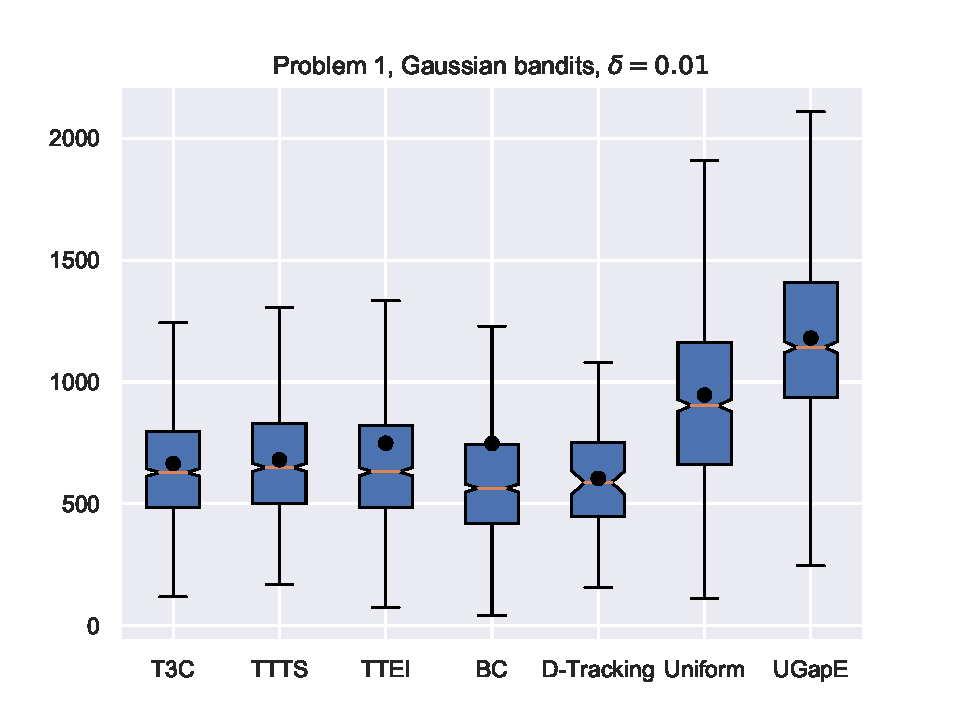
\includegraphics[clip, width= 0.24\textwidth]{Chapter3/img/gaussian1.pdf}
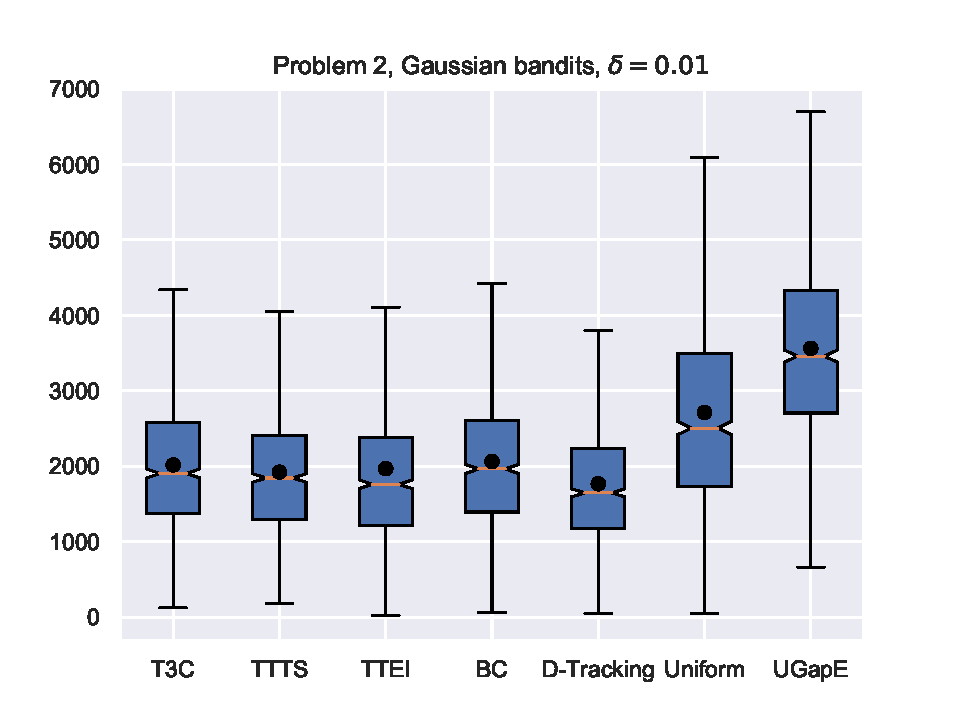
\includegraphics[clip, width= 0.24\textwidth]{Chapter3/img/gaussian2.pdf}
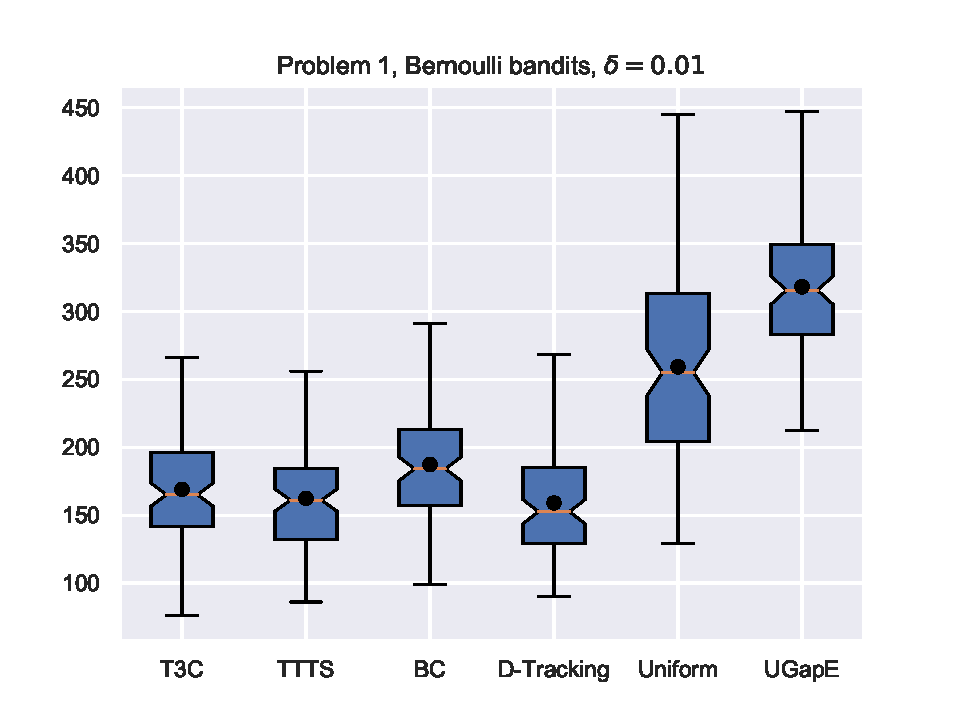
\includegraphics[clip, width= 0.24\textwidth]{Chapter3/img/bernoulli1.pdf}
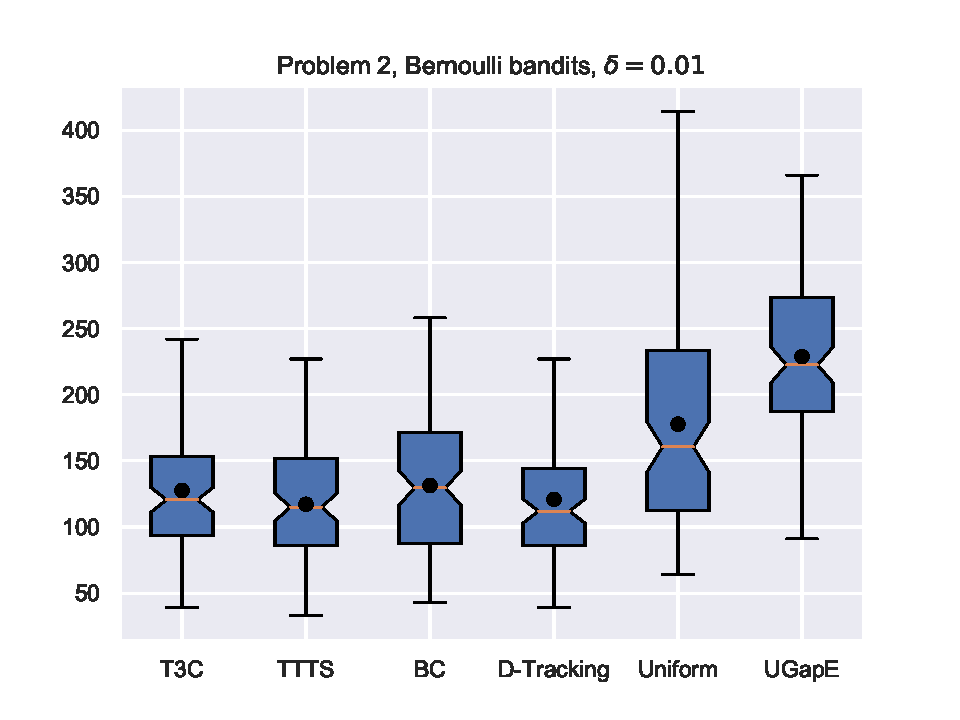
\includegraphics[clip, width= 0.24\textwidth]{Chapter3/img/bernoulli2.pdf}
\caption{Sample complexity of different BAI sampling rules over some random problem instances. Black dots represent means and oranges lines represent medians.}
\label{fig:confidence}
\end{figure*}

\begin{table*}[t!]
\centering
\small
%\def\arraystretch{1.2}
\begin{tabular}{|c|c|c|c|c|c|c|c|}
 \hline
 \textbf{Sampling rule} & \TCC & \TTTS & \TTEI & \BC & \DT & \texttt{Uniform} & \UGapE \\
 \hline
 \textbf{Execution time (s)} & $1.6\times 10^{-5}$ & $2.3\times 10^{-4}$ & $1\times 10^{-5}$ & $1.4\times 10^{-5}$ & $1.3\times 10^{-3}$ & $6\times 10^{-6}$ & $5\times 10^{-6}$ \\
 \hline
\end{tabular}
\caption{Average execution time in seconds for different BAI sampling rules.}
\label{table:time}
\end{table*}


\section{Optimal Posterior Convergence
}\label{sec:bayesian}

Recall that $a_{n, I^\star}$ denotes the posterior mass assigned to the event that action $I^\star$ (i.e.\ the true optimal arm) is optimal at time $n$. As the number of observations tends to infinity, we desire that the posterior distribution converges to the truth. In this section we show equivalently that the posterior mass on the complementory event, $1 - a_{n, I^\star}$, the event that arm $I^\star$ is not optimal, converges to zero at an exponential rate, and that it does so at optimal rate $\Gamma_{\beta}^\star$. 

\citet{russo2016ttts} proves a similar theorem under three confining boundedness assumptions (cf.\,\citealt{russo2016ttts}, Asssumption 1) on the parameter space, the prior density and the (first derivative of the) log-normalizer of the exponential family. Hence, the theorems in \cite{russo2016ttts} do not apply to the two bandit models most used in practise, which we consider in this paper: the Gaussian and Bernoulli model. 

In the first case, the parameter space is unbounded, in the latter model, the derivative of the log-normalizer (which is $e^{\eta} / (1 + e^\eta)$) is unbounded. Here we provide two theorems, proving that under \TTTS, the optimal, exponential posterior convergence rates are obtained for the Gaussian model with uninformative (improper) Gaussian priors (proof given in Appendix~\ref{app:posterior_gaussian}), and the Bernoulli model with $\cB eta(1,1)$ priors (proof given in Appendix~\ref{app:posterior_beta}).

\begin{restatable}{theorem}{restateposteriorgaussian}\label{thm:posterior_gaussian}
    Under \TTTS, for Gaussian bandits with improper Gaussian priors, it holds almost surely that 
    \[
        \lim_{n\rightarrow{\infty}} -\frac{1}{n}\log(1-a_{n,I^\star}) = \Gamma_{\beta}^\star.
    \]
\end{restatable}

\begin{restatable}{theorem}{restateposteriorbernoulli}\label{thm:posterior_bernoulli}
	Under \TTTS, for Bernoulli bandits and uniform priors, it holds almost surely that
	\[
	\lim_{n\rightarrow{\infty}} -\frac{1}{n}\log(1-a_{n,I^\star}) = \Gamma_{\beta}^\star.
	\]
\end{restatable}


%!TEX root = ../Chapter3.tex
\begin{figure*}[t!]
 \centering
 \includegraphics[clip, width= 0.3\textwidth]{Chapter3/img/bai_sin_0-1}
 \includegraphics[clip, width= 0.3\textwidth]{Chapter3/img/bai_sin_0-01}
 \includegraphics[clip, width= 0.3\textwidth]{Chapter3/img/bai_sin_0-0001}
 \caption{Sample complexity of different linear BAI sampling rules over the usual counter-example with $\delta=0.1, 0.01, 0.0001$ respectively. CG = \LGC,  Lk = \LG, RR = uniform sampling, fix = tracking the fixed weights, GS = \XYS with $\gopt$-allocation, XYS = \XYS with $\xyopt$-allocation, LG = \LGapE. The mean stopping time is represented by a black cross.}
 \label{fig:sample_complexity_1}
\end{figure*}

\begin{figure*}[t!]
 \centering
 \includegraphics[clip, width= 0.24\textwidth]{Chapter3/img/bai_dim_6}
 \includegraphics[clip, width= 0.24\textwidth]{Chapter3/img/bai_dim_8}
 \includegraphics[clip, width= 0.24\textwidth]{Chapter3/img/bai_dim_10}
 \includegraphics[clip, width= 0.24\textwidth]{Chapter3/img/bai_dim_12}
 \caption{Sample complexity of different linear BAI sampling rules over random unit sphere vectors with $d=6, 8, 10, 12$ from left to right.}
 \label{fig:sample_complexity_2}
\end{figure*}

\section{Experiments}\label{sec:lgc.experiments}
Besides our algorithms, we implement the following algorithms, all using the same stopping rule (more discussion given in Appendix~\ref{app:lgc.stopping}): uniform sampling, the greedy version of \XYS (including $\gopt$-allocation and $\xyopt$-allocation), \XYA, and the greedy version of \LGapE. We skip \GLUCB/\GLGapE since they are more or less equivalent to \LGapE in the scope of this paper.
\vspace{-0.3cm}
\paragraph{The usual hard instance.}
Usual sampling rules for classical BAI may not work for the linear case. This can be understood on a well-studied instance already discussed by~\citet{soare2014linear,xu2018linear}, which encapsulates the difficulty of BAI in a linear bandit, and thus is the first instance on which we test our algorithms. In this instance, arms are the canonical basis  $a_1 = e_1, a_2 = e_2, a_d = e_d$, plus an additional disturbing arm $a_{d+1} = (\cos(\alpha), \sin(\alpha), 0, \ldots, 0)^\top$, and a true regression parameter $\theta$ equal to $e_1$. In this problem, the best arm is always $a_1$, but when the angle $\alpha$ is small, the disturbing arm $a_{d+1}$ is hard to discriminate from $a_1$. As already argued by~\citet{soare2014linear}, an efficient sampling rule for this problem instance would rather pull $a_2$ in order to reduce the uncertainty in the direction $a_1-a_{d+1}$. Naive adaptation of classical BAI algorithms cannot deal with that situation naturally. We further use a simple set of experiments to justify that intuition. We run our two algorithms and the one of~\citet{degenne2019game} that we call \texttt{DKM} over the problem instance whence $d=2$, $\delta=0.01$ and $\alpha=0.1$. We show the number of pulls for each arm averaged over 100 replications of experiments in Table~\ref{table:pulls}. We see that, indeed, \texttt{DKM} pulls too much $a_3$, while our algorithms focus mostly on $a_2$.


\begin{table}[th]\centering
%\def\arraystretch{1.2}
\begin{tabular}{|c|c|c|c|}
 \hline
 & \LG & \LGC & \texttt{DKM} \\
 \hline
 \textbf{$a_1$} & $1912$ & $1959$ & $1943$ \\
 \hline
 \textbf{$a_2$} & $5119$ & $4818$ & $4987$ \\
 \hline
 \textbf{$a_3$} & $104$ & $77$ & $1775$ \\
 \hline
 \textbf{Total} & $7135$ & $\bf{6854}$ & $8705$ \\
 \hline
\end{tabular}
\caption{Average number of pulls of \LG and \LGC (against \texttt{DKM}) for each arm.}
\label{table:pulls}
\end{table}

\vspace{-0.3cm}
\paragraph{Comparison of different complexities.}
We use the previous setting to illustrate various complexities differ in practice. In Table~\ref{table:optimal_weights} we compare the different complexities mentioned in this paper: the characteristic time $\Tstar(\theta)$ and its associated optimal weights $\wstar_{\cA\cBstar(\theta)}$, the $\xyopt$-complexity and its associated optimal design $\wstar_{\xyopt}$, the G-optimal complexity $\gopt$ and its associated optimal design $\wstar_{\cA\cA}$. For each weight vector $w \in\{\wstar_{\cA\cBstar(\theta)},w_{\xyopt}, w_{\gopt}\}$,
 we also provide the lower bound $T_w$ given by Therorem~\ref{th:lb_genral}, i.e.
 \[
 T_w = \max_{a\neq \astar(\theta)} \frac{\big\langle \theta, \astar(\theta)-a\big\rangle^2}{2\normm{\astar(\theta)-a}_{V_w^{-1}}^2} \log(1/\delta).
\]
In particular we notice that targeting the proportions of pulls $w_{\xyopt}, w_{\gopt}$ leads to a much larger lower bound than the one obtained with the optimal weights.
\begin{table}[th]
\centering
%\def\arraystretch{1.2}
\begin{tabular}{|c|c|c|c|}
 \hline
   & $\wstar_{\cA\cBstar}$ & $\wstar_{\xyopt}$  & $\wstar_{\gopt}$   \\
 \hline
 \textbf{$a_1$} & $0.047599$ & $0.499983$ & $0.499983$ \\
 \hline
 \textbf{$a_2$} & $0.952354$ & $0.499983$ & $0.499983$ \\
 \hline
 \textbf{$a_3$} & $0.000047$ & $0.000033$ & $0.000033$ \\
 \hline
 \textbf{$T_w$} & $369$ & $2882$ & $2882$ \\
 \hline
   & $\Tstar(\theta)$ & $2\xyopt/\DeltaMin^2$ & $8\gopt/\DeltaMin^2$\\
 \hline
  \textbf{Complexity} & $0.124607$ & $32.0469$ & $64.0939$ \\
 \hline
\end{tabular}
\caption{Optimal weights for various complexities with $\DeltaMin= 0.0049958$.}
\label{table:optimal_weights}
\end{table}

\paragraph{Comparison with other algorithms.}
Finally we benchmark our two sampling rules against others from the literature. %Note that the main purpose of this paper is to propose algorithms with asymptotic optimality while being practically usable, but we do not claim to have the best performing ones.
We test over two synthetic problem instances, with the first being the previous counter-example. We set $d=2$, $\alpha=\pi/6$. Fig.~\ref{fig:sample_complexity_1} shows the empirical stopping time of each algorithms averaged over 100 runs, with a confidence level $\delta=0.1, 0.01, 0.0001$ from left to right. Our two algorithms show competitive performance (the two leftmost boxes on each plot), and are only slightly worse than \LGapE.

For the second instance, we consider 20 arms randomly generated from the unit sphere $\mathbb{S}^{d-1}\eqdef\{a\in\R^d; \normm{a}_2=1\}$. We choose the two closest arms $a, a'$ and we set $\theta = a + 0.01(a'-a)$ so that a is the best arm. This setting has already been considered by~\citet{tao2018alba}. We report the same box plots over 100 replications as before with increasing dimension in Fig.~\ref{fig:sample_complexity_2}. More precisely, we set $d=6, 8, 10, 12$ respectively, and always keep a same $\delta = 0.01$. Our algorithms consistently show strong performances compared to other algorithms apart from \LGapE. Moreover, we can see that in these random examples, \LGC works better than the non-confexified one, and is even competitive compared to \LGapE.

We stress that although the main focus of this paper is theoretical, with algorithms that are asymptotically optimal, our methods are also competitive with earlier algorithms experimentally.


%!TEX root = ../Chapter3.tex
\section{Discussion}\label{sec:t3c.discussion}

We have advocated the use of a Bayesian sampling rule for BAI. In particular, we proved that \TTTS and a computationally advantageous approach \TCC, are both $\beta$-optimal in the fixed-confidence setting, for Gaussian bandits. 
%Our analysis applies to Gaussian bandits, but could be extended to more distributions for which posterior tails bounds are available. 
We further extended the Bayesian optimality properties established by \cite{russo2016ttts} to more practical choices of models and prior distributions. 


In order to be optimal, the sampling rules studied in this paper would need to use the oracle tuning $\beta^\star =\argmax_{\beta \in [0,1]} \Gamma_\beta^\star$, which is not feasible. In future work, we will investigate an efficient online tuning of~$\beta$ to circumvent this issue. We also plan to investigate the extension of \TCC to more general pure exploration problems, as an alternative to approaches recently proposed by~\citet{menard2019lma,degenne2019game}.

Finally, it is also important to study Bayesian sampling rules in the fixed-budget setting which is more plausible in many application scenarios such as applying BAI for automated machine learning~\citep{hoffman2014bayesgap,li2017hyperband,shang2019dttts}.
\vfil


% \newpage
% \bibliographystyle{plainnat}
% \bibliography{Major}
% \newpage

	%%%%%%%%%%%%%%%%%%%%%%%%%%%%%%%%%%%%%%%%%%%%%%%%%%%%%%%%%%%%%%%%%%%%%%%%%%%%%%%%%%%%%%%%%%%%%%
%%									Chapitre 4											%
%%%%%%%%%%%%%%%%%%%%%%%%%%%%%%%%%%%%%%%%%%%%%%%%%%%%%%%%%%%%%%%%%%%%%%%%%%%%%%%%%%%%%%%%%%%%%

\chapter{Playground of Linear Best-Arm Identification}\label{CHAP:LGC}
	\citationChap{
		Et c'est là que jadis, à quinze ans révolus\\
		A l'âge où s'amuser tout seul ne suffit plus\\
		Je connus la prime amourette\\
		Auprès d'une sirène, une femme-poisson\\
		Je reçus de l'amour la première leçon\\
		Avalai la première arête
	}{Georges Brassens}
	\minitoc
	\newpage

%%%%%%%%%%%%%%%%%%%%%%%%%%%%%%%%%%%%%%%%%%%%%%%%%%%%%%%%%%%%%%%%%%%%%%%%%%%%%%%%%%%%%%%%%%%%%



% Début du chapitre
\addtocontents{toc}{\protect\setcounter{tocdepth}{1}}
%!TEX root = ../Chapter3.tex
\section{Introduction}\label{sec:lgc.intro}

%Multi-armed bandits (MAB) probe fundamental \emph{exploration-exploitation} trade-offs in sequential decision learning. We study the pure exploration framework, from among different MAB models, which is subject to the maximization of information gain after an exploration phase. 

Following the previous chapter, we put our focus onto a natural extension of the vanilla BAI problem. In particular, we are interested in the case where noisy linear payoffs depending on some regression parameter $\btheta$ are assumed. Inspired by~\citet{degenne2019game}, we treat the problem as a \emph{two-player zero-sum} game between the agent and the nature (in a sense described in Section~\ref{sec:lgc.lower_bound}), and we search for algorithms that are able to output a correct answer with high confidence to a given query using as few samples as possible.

In this chapter, we consider a general pure-exploration setting (see Appendix~\ref{app:lgc.examples} for details). Nevertheless, for the sake of simplicity, in the main text we primarily focus on BAI.  For stochastic bandits, BAI has been studied within two major theoretical frameworks. The first one,  \emph{fixed-budget} BAI, aims at minimizing the probability of misidentifying the optimal arm within a given number of pulls~\citep{audibert2010budget}. In this work, we consider another setting, \emph{fixed-confidence} BAI, introduced by~\citet{even-dar2003confidence}. Its goal is to ensure that the algorithm returns a wrong arm with probability less than a given risk level, while using a small total number of samples before making the decision. %Note that these two frameworks are very different in general and do not share transferable regret bounds (see~\citealt{carpentier2016budget} for an additional discussion).
%Existing fixed-confidence algorithms mostly depend on the risk parameter $\delta \in (0,1)$ \todo{what does that mean?}.

Existing fixed-confidence algorithms are either elimination-based such as \SE~\citep{karnin2013sha}, rely on confidence intervals such as \UGapE~\citep{gabillon2012ugape}, or follow plug-in estimates of the optimal pulling proportions by a lower bound such as \Track~\citep{garivier2016tracknstop}. We pay particular attention to the first two since they have been extended to the linear setting, which is the focus of this paper.
%\textcolor{blue}{mv: possible selling point:  this was has been identified as a challenging ... the usual simple counter-example... that shows that the typical
%"tricks" don't work well and methods need to work around it. This comes for a price weird complexity terms - unclear to explain the difficulty - (max term in the Soare paper).
%By being "'optimal" we "naturally" avoid this "pitfall".
%}
In particular, a natural extension of pure exploration to linear bandits. Linear bandits were first investigated by~\citet{auer2002linear} in the stochastic setting for \emph{regret minimization} and later considered for fixed-confidence BAI problems by~\citet{soare2014linear}.
%\vspace{-0.4cm}
\paragraph{Linear bandits.}
We consider a \emph{finite-arm linear bandit} problem, where the collection of arms $\cA\subset \R^d$ is given  with $|\cA|=A$, and spans $\R^d$. We assume that $\forall a\in\cA, \normm{a}\leq L$, where $\normm{a}$ denotes the Euclidean norm of the vector $a$. The learning protocol goes as follows: for each round $1\leq t \leq T,$ the agent chooses an arm $a_t\in\cA$ and observes a noisy sample
\[
Y_t =\langle \theta,a_t\rangle +\eta_t\,,
\]
where $\eta_t \sim \cN(0,\sigma^2)$ is conditionally independent from the past and $\theta$ is some unknown regression parameter. For the sake of simplicity, we use $\sigma^2 = 1$ in the rest of this paper.

\paragraph{Pure exploration for linear bandits.}
We assume that $\theta$ belongs to some set $\cM\subset\R^d$ known to the agent. % s.t.\,$\forall \theta\in\cM, \normm{\theta}\leq M$.
For each parameter a \emph{unique correct answer} is given by the function $\istar: \cM \to \cI$ among the $I = |\cI|$ possible ones (the extension of pure exploration to multiple correct answers is studied by~\citealt{degenne2019pure}). Given a parameter~$\theta$, the agent then aims to find the correct answer $\istar(\theta)$ by interacting with the finite-armed linear bandit environment parameterized by~$\theta$.

In particular, we detail the setting of BAI for which the objective is to identify the arm with the largest mean. That is, the correct answer is given by $\istar(\theta)=\astar(\theta)\eqdef \argmax_{a\in\cA} \langle\theta,a\rangle$ for $\theta\in\cM = \R^d$ and the set of possible correct answers is $\cI = \cA$. We provide other pure-exploration examples in Appendix~\ref{app:lgc.examples}.

\paragraph{Algorithm.}
Let $\cF_{t}=\sigma (a_1,Y_1,\ldots, a_t,Y_t)$ be the information available to the agent after $t$ round. A deterministic pure-exploration algorithm under the fixed-confidence setting is given by three components: (1) a \emph{sampling rule} $(a_t)_{t\geq 1}$, where $a_t\in\cA$ is $\cF_{t-1}$-measurable, (2) a \emph{stopping rule} $\tau_\delta$, a stopping time for the filtration $(\cF_t)_{t\geq 1}$, and (3) a \emph{decision rule} $\hi\in \cI$ which is $\cF_{\tau_\delta}$-measurable.
Non-deterministic algorithms could also be considered by allowing the rules to depend on additional internal randomization. The algorithms we present are deterministic.

\paragraph{$\delta$-correctness and fixed-confidence objective.}
An algorithm is $\delta$-correct if it predicts the correct answer with probability at least $1-\delta$, precisely if $\P_\theta \big(\hi \neq \istar(\theta)\big) \leq \delta$ and $\tau_\delta < +\infty$ almost surely for all $\theta \in\cM$. Our goal is to find a $\delta$-correct algorithm that minimizes the \emph{sample complexity}, that is,  $\E_\theta[\tau_\delta]$ the expected number of sample needed to predict an answer.

Pure exploration (in particular BAI) for linear bandits has been previously studied by
~\citet{soare2014linear,tao2018alba,xu2018linear,zaki2019maxoverlap,fiez2019transductive,kazerouni2019glb}. They all consider the fixed-confidence setting. To the best of our knowledge, only~\citet{hoffman2014bayesgap} study the problem with a fixed-budget.

Beside studying fixed-confidence sample complexity,~\citet{garivier2016tracknstop} and some subsequent works~\citep{qin2017ttei,shang2020t3c} investigate a general criterion of judging the optimality of a BAI sampling rule: Algorithms that achieve the minimal sample complexity when~$\delta$ tends to zero are called asymptotically optimal. \citet{menard2019lma} and~\citet{degenne2019game} further study the problem in a game theoretical point of view, and extend the asymptotic optimality to the general pure exploration for structured bandits. Note that a naive adaptation of the algorithm proposed by~\citet{degenne2019game} may not work smoothly in our setting. In this paper we use some different confidence intervals that benefit better from the linear structure.

\paragraph{Contributions.}
\textbf{1)}
We provide new insights on the complexity of linear pure exploration bandits. In particular, we relate the asymptotic complexity of the BAI problem and other measures of complexity inspired by optimal design theory, which were used in prior work.
\textbf{2)}
We develop a saddle-point approach to the lower bound optimization problem, which also guides the design of our algorithms. In particular we highlight a new insight on a convex formulation of that problem. It leads to an algorithm with a more direct analysis than previous lower-bound inspired methods.
\textbf{3)}
We obtain two algorithms for linear pure exploration bandits in the fixed-confidence regime. Their sample complexity is asymptotically optimal and their empirical performance is competitive with the best existing algorithms.

%--- new insight on the complexity
%
%--- presenting a saddle point of view
%
%--- insight leads into convexication
%
%--- main result + 2 algos +  2 theorems proving that they are asymptotically optimal


%!TEX root = ../Chapter4.tex
\section{Problem Setting and Assumptions}\label{sec:lgc.formulation}

In this section, we recall the problem setting of linear bandits as well as linear bandits BAI. In particular, we specify the assumptions used in this chapter.

\paragraph{Linear bandits.}
We consider a finitely-armed linear bandit problem, where the collection of arms $\cX\eqdef\{\bx_1,\cdots,\bx_K\}\subset \R^d$ is given with $|\cX|=K$, and spans $\R^d$. When there is no ambiguity, we can also use the index $i\in[K]$ to represent arm $\bx_i$. The (unknown) mean of each arm is given by
\[
    \mu_i = \bx_i\transpose\btheta\,.
\]

\begin{assumption}\label{ass:lgc.bounded_arm}
\begin{leftbar}[assumptionbar]
    We assume that $\exists L>0$, $\forall \bx\in\cX, \normm{\bx}\leq L$, where $\normm{\bx}$ denotes the Euclidean norm of the vector $\bx$.
\end{leftbar}
\end{assumption}

The learning protocol (see also Definition~\ref{def:mab.linear_bai}) goes as follows: for each round $n$, the learner chooses an arm $\hbx_n\in\cX$ and observes a noisy sample
\[
    r_n = \hbx_n\transpose\btheta +\epsilon_n\,,
\]
where $\epsilon_n$ is the noise and $\btheta$ is the true regression parameter (unknown to the learner).
\begin{assumption}\label{ass:lgc.noise}
\begin{leftbar}[assumptionbar]
    We assume that $\epsilon_n \sim \cN(0,\sigma^2)$ is conditionally independent from the past\,.
\end{leftbar}
\end{assumption}
For the sake of simplicity, we set $\sigma^2 = 1$ in the rest of this paper.

\paragraph{Best-arm identification for linear bandits.}
We assume that $\btheta$ belongs to some parameter set $\Theta\subset\R^d$ known to the learner. Recall that in a pure exploration game, given a parameter $\btheta$, the learner aims to find the correct answer $\Istar(\btheta)\in\cI$ by interacting with the finite-armed linear bandit environment parameterized by $\btheta$ (see also Section~\ref{sec:mab.extensions.pure}).

In particular, we are interested in BAI for which the objective is to identify the arm with the largest mean. That is, the correct answer given $\btheta$ is given by 
\[
\Istar(\btheta) = \bx^\star(\btheta) \eqdef \argmax_{\bx\in\cX} \bx\transpose\btheta
\]
for $\btheta\in\Theta = \R^d$ and the set of possible correct answers is $\cI = \cX$. When clear from the context, we can simply denote $\bx^\star(\btheta)$ by $\bx$.

\paragraph{Algorithm.}
Let $\cF_{n}=\sigma (\hbx_1,r_1,\cdots, \hbx_n,r_n)$ be the information available to the learner after $n$ round. We restate the definition of a BAI algorithm under the fixed-confidence setting, which is given by three components: (1) a \emph{sampling rule} $(\hbx_n)_{n\geq 1}$, where $\hbx_n\in\cX$ is $\cF_{n-1}$-measurable, (2) a \emph{stopping rule} $\tau_\delta$, a stopping time for the filtration $(\cF_n)_{n\geq 1}$, and (3) a \emph{decision rule} $J_\tau\in \cX$ which is $\cF_{\tau_\delta}$-measurable.
%Non-deterministic algorithms could also be considered by allowing the rules to depend on additional internal randomization. The algorithms we present are deterministic.

\paragraph{$\delta$-correctness and fixed-confidence objective.}
As already stated several times in the previous chapters, we say that an algorithm is $\delta$-correct if it predicts the correct best arm with probability at least $1-\delta$, precisely if $\PPt{\big(\bx_{J_\tau} \neq \Istar(\btheta)\big) \leq \delta}$ and $\tau_\delta < +\infty$ almost surely for all $\btheta \in\Theta$. Our goal is to find a $\delta$-correct algorithm that minimizes the \emph{sample complexity}, that is,  $\E_\btheta[\tau_\delta]$ the expected number of sample needed to predict an answer.

\paragraph{Linear estimator.}
A crucial step in linear bandits is to estimate the regression parameter $\btheta$. Let $\bX_n=(\hat{\bx}_1,\ldots,\hat{\bx}_n)$ be a sequence of sampled arms, and $\br_n=(r_1,\ldots,r_n)$ be the corresponding observations. To estimate $\btheta^\star$ based on the adaptive sequence of observations $\br_n$, one may use the \gls{regularized least-square estimation}
\begin{align}\label{eq:update_mean}
    \hat{\btheta}_n^{\lambda} = (\lambda \1_d + \bA_{\bX_n})^{-1}\bb_{\bX_n}\,,
\end{align}
where $\bA_{\bX_n}$ and $\bb_{\bX_n}$ are the design matrix and the response vector respectively given by
\[
    \bA_{\bX_n} \eqdef \sum_{t=1}^n \hat{\bx}_t\hat{\bx}_t\transpose, \quad \bb_{\bX_n} \eqdef \sum_{t=1}^n \hat{\bx}_t r_t\,,
\]
and $\lambda\in\R$ is the regularization parameter. When clear from the context, we can simply denote $\bA_{\bX_n}$ by $\bA_n$ and $\bb_{\bX_n}$ by $\bb_n$.

\paragraph{Useful notation.}
The fixed-confidence optimality, as proved by~\cite{garivier2016tracknstop,russo2016ttts}, is related to the \emph{proportion vector} of pulls of each arm that we denote by $\bomega = (\omega_1,\ldots,\omega_K)$, where $\bomega\in\Sigma_K \eqdef \{\bomega : \sum_{i=1}^K \omega_i = 1\}$. Given a vector of proportions $\bomega$, we can define a counterpart of the design matrix 
\[
    \bLambda_{\bomega} \eqdef \sum_{i=1}^K \omega_i\bx_i\bx_i\transpose.
\]

It is easy to switch between the design matrix and the proportion vector. Indeed, given a sequence of sampled arms $\bX_n$, the corresponding proportion vector can be written as
\[
    \forall i\in [K], \quad \omega_{\bX_n,i} = \frac{T_{n+1,i}}{n},
\]
where recall that $T_{n,i} \eqdef \sum_{t=1}^{n-1} \1\{\hat{\bx_t} = i\}$ is the number of pulls of arm $i$ before round $n$. Therefore, the corresponding design matrix can be written as $\bA_{\bX_n}=n\bLambda_{\bomega_{\bX_n}}$.

Another important notation that we employ ceaselessly is the Mahalanobis norm which is defined, given a positive semi-definite matrix $\bA\in\R^{d\times d}$, by
\[
    \forall \bx\in\R^d, \quad \normm{\bx}_{\bA} = \sqrt{\bx\transpose\bA\bx}.
\]


%!TEX root = ../Chapter4.tex
\section{Related Work}\label{sec:lgc.related_work}

We survey previous work on linear BAI. The major focus is put on sampling rules in this section. We stress that all the stopping rules employed in the linear BAI literature are equivalent up to the choice of their exploration rate (More discussion in Appendix~\ref{app:lgc.stopping}). As aforementioned, existing sampling rules are either based on \SE or \UGapE. Elimination-based sampling rules usually operate in phases and progressively discard sub-optimal directions. Gap-based sampling rules always play the most informative arm that reduces the uncertainty of the gaps between the empirical best arm and the others.

\paragraph{\XYS and \XYA.} \citet{soare2014linear} first propose a static allocation design \XYS that aims at reducing the uncertainty of the gaps of all arms. More precisely, it requires to either solve the $\xyopt$-complexity or use a \emph{greedy} version that pulls the arm 
\[
    \argmin_{\bx\in\cX} \max_{\by\in\cY_{\texttt{dir}}} \normm{\by}_{\bLambda_{\bomega}^{-1}}^2
\]
at the cost of having no guarantees. An elimination-like alternative called \XYA is proposed then to overcome that issue. We say elimination-like since \XYA does not discard arms once and for all, but reset the active arm set at each phase. These two algorithms are the first one being linked to $\gopt$-optimality, but are not asymptotically optimal.

\paragraph{\ALBA.} \ALBA is also an eliminations-based algorithm designed by~\citet{tao2018alba} that improves over \XYA by a factor of $d$ in the sample complexity using a tighter elimination criterion.
\vspace{-0.2cm}

\paragraph{\RAGE.} \citet{fiez2019transductive} extend \XYS and \XYA to a more general transductive bandits setting. \RAGE is also elimination-based and requires the computation of $\xyopt$-complexity at each phase.

\paragraph{\LGapE and variants.} \LGapE~\citep{xu2018linear} is the first gap-based sampling rule for linear BAI. \LGapE is inspired by \UGapE~\citep{gabillon2012ugape}. It is, however, not clear whether \LGapE is asymptotically optimal or not. Similar to \XYS, \LGapE either requires to solve a time-consuming optimization problem at each step, or can use a greedy version that pulls arm 
\[
    \argmin_{\bx\in\cX} \normm{\bx_{i_n}-\bx_{j_n}}_{(\bA_n+\bx\bx\transpose)^{-1}}^2
\]
instead, again at the cost of losing guarantees. Here $i_n = \Istar(\hat\btheta_n)$ and $\hbx_{j_n}$ is the most ambiguous arm w.r.t. $\hbx_{i_n}$, i.e. 
\[
    \argmax_{j\neq i_n} (\bx_{j}-\bx^\star(\hat\btheta_n^\lambda))\transpose\hat\btheta_n^\lambda + \normm{\bx^\star(\hat\btheta_n^\lambda) - \bx_{j_n}}_{\bA_n^{-1}} \sqrt{2d_{n,\delta}}\,,
\]
with $d_{n,\delta}$ the stopping rule threshold.

On the other hand,~\citet{zaki2019maxoverlap} propose a new algorithm based on \LUCB. With a careful examination, we note that the sampling rule of \GLUCB is equivalent to that of the greedy \LGapE using the Sherman-Morrison formula. Later, \citet{kazerouni2019glb} provide a natural extension of \LGapE to the \emph{generalized linear bandits} setting, where the rewards depend on a strictly increasing \emph{inverse link function}. \GLGapE reduces to \LGapE when the inverse link function is the identity function.

\paragraph{Summary.}
It is worth noting that all the sampling rules presented here depend on $\delta$ (except \XYS), while we aim to design sampling rules that are $\delta$-free which is appealing for applications as argued by~\citet{jun2016atlucb}. Also all the guarantees in the literature are of the form $C\log(\delta) + O\big(\log(1/\delta)\big)$ for a constant $C$ that is strictly larger than $\Tstar(\theta)^{-1}$.

In the next, we present a set of algorithms using different design patterns that aim to address linear bandits BAI, whilst trying to be asymptotically optimal.


%!TEX root = ../Chapter3.tex
\section{Fixed-Confidence Optimality}\label{sec:lgc.lower_bound}

As first stated by~\cite{soare2014linear}, we only consider a finite number of arms and we restrict to bandits  with Gaussian rewards and conjugate (Gaussian) priors in this work. Our objective is to propose a BAI strategy that outputs a guess which is accurate enough. Formally, given a risk level $\delta$, we want to show that
\[
  \PP{a_{\tau_\delta}\neq \bx^\star} \leq \delta,
\]
while minimizing the expected number of samples $\EE{\tau_\delta}$ that is required. That is the so-called \emph{fixed-confidence} best-arm identification introduced by~\cite{even-dar2003confidence}.

\subsection{Lower bound}

In this section we extend the lower bound of \citet{garivier2016tracknstop}, to hold for \emph{pure exploration in finitely-armed linear bandit} problems.

\paragraph{Lower bound} A general lower bound on the sample complexity in the fixed-confidence setting is given by~\cite{garivier2016tracknstop}, which states that for any $\delta$-correct strategy, we have
\[
    \EE{\tau_\delta} \geq T^\star(\bmu)\log(\frac{1}{3\delta}),
\]
for a given bandit model $\bmu$ and a given confidence level $\delta$. 

\begin{proposition}
In the linear case, the quantity $T^\star(\bmu)$ is written as
\[
  T^\star(\bmu) \eqdef \inf_{\bomega\in\Sigma_K}\max_{\bx\neq \bx^\star} \frac{2\sigma^2\normm{\bx^\star - \bx}^2_{\bLambda_{\bomega}^{-1}}}{(\bx\transpose\btheta^\star-(\bx^\star)\transpose\btheta^\star)^2}.
\]
\end{proposition}

\begin{proof}
Let $\texttt{Alt}(\btheta) \eqdef \{\btheta':\exists \bx\in\cX, \bx\transpose\btheta'>(\bx^\star)\transpose\btheta'\}$, and we obtain
\begin{align*}
    T^\star(\bmu)^{-1} &= \sup_{\bomega\in\Sigma_K}\inf_{\btheta'\in\texttt{Alt}(\btheta^\star)}\sum_{i=1}^K \omega_i d(\mu_i;\mu_i')\\
                       &= \sup_{\bomega\in\Sigma_K}\min_{\bx\neq\bx^\star}\inf_{\bx\transpose\btheta'>(\bx^\star)\transpose\btheta'} \frac{\normm{\btheta^\star-\btheta'}_{\bLambda_{\bomega}}^2}{2\sigma^2}.
\end{align*}
Then we introduce the Lagrangian with $\eta$ as the Lagrange multiplier, and it then becomes
\begin{align*}
    T^\star(\bmu)^{-1} &= \sup_{\bomega\in\Sigma_K}\min_{\bx\neq\bx^\star}\inf_{\btheta'}\sup_{\eta>0} \frac{\normm{\btheta^\star-\btheta'}_{\bLambda_{\bomega}}^2}{2\sigma^2} - \eta(\bx-\bx^\star)\transpose\btheta',
\end{align*}
and the inner expression attains its minimum when it comes
\[
    \frac{1}{\sigma^2}\bLambda_{\bomega}(\btheta^\star-\btheta') = \eta(\bx^\star-\bx),
\]
which implies
\begin{align*}
    T^\star(\bmu)^{-1} &=
    \sup_{\bomega\in\Sigma_K}\min_{\bx\neq\bx^\star}\sup_{\eta>0} \eta(\bx^\star-\bx)\transpose\btheta^\star - \frac{\eta^2\normm{\bx-\bx^\star}_{\bLambda_{\bomega}^{-1}}}{2\sigma^2}\\
    &= \sup_{\bomega\in\Sigma_K}\min_{\bx\neq\bx^\star}\frac{(\bx\transpose\btheta^\star-(\bx^\star)\transpose\btheta^\star)^2}{2\sigma^2\normm{\bx^\star - \bx}^2_{\bLambda_{\bomega}^{-1}}}.
\end{align*}
\end{proof}

Using the same lower bound techniques, one can also prove that under any $\delta$-correct strategy satisfying $T_{n,I^\star}/n \rightarrow \beta$ for a given $\beta$,
\[
    \liminf_{\delta \rightarrow 0}\frac{\EE{\tau_\delta}}{\ln(1/\delta)} \geq T^\star_\beta(\bmu),
\]
where $T^\star_\beta(\bmu)$ is defined in the same way as $T^\star(\bmu)$, but restricted to the constraint $\omega_{I^\star}=\beta$,
\[
    T^\star_{\beta}(\bmu) \eqdef \inf_{\bomega\in\Sigma_K,\omega_{I^\star}=\beta}\max_{\bx\neq \bx^\star} \frac{2\sigma^2\normm{\bx^\star - \bx}^2_{\bLambda_{\bomega}^{-1}}}{(\bx\transpose\btheta^\star-(\bx^\star)\transpose\btheta^\star)^2}.
\]

\paragraph{Notion of optimality}
We can now define a notion of optimality upon $T^\star_\beta(\bmu)$. A BAI strategy is called \emph{optimal} in the fixed-confidence setting if it satisfies
\[
    \limsup_{\delta \rightarrow 0}\frac{\EE{\tau_\delta}}{\ln(1/\delta)} \leq T^\star(\bmu).
\]
And a relaxed notion of optimality that depends on $\beta$ can be also defined. A BAI strategy is called \emph{$\beta$-optimal} if it satisfies 
\[
    \frac{T_{n,I^\star}}{n}\rightarrow \beta \quad \text{and} \quad \limsup_{\delta \rightarrow 0}\frac{\EE{\tau_\delta}}{\ln(1/\delta)} \leq T^\star_\beta(\bmu).
\]

\paragraph{Alternative.}
For any answer $i\in\cI$ we define \emph{the alternative to i}, denoted by $\neg i$ the set of parameters where the answer $i$ is not correct, i.e.
$%\[
\neg i \eqdef \{\theta\in\cM:\ i\neq\istar(\theta)\}\,.
$%\]

We also define, for any $w\in(\R^+)^A$, the design matrix
\[V_w \eqdef \sum_{a\in \cA} w^a a a^\top\,.\]
Further, we define $\normm{x}_V\eqdef \sqrt{x^\top Vx}$ for $x\in\R^d$ and a symmetric positive matrix $V\in\R^{d\times d}$. Note that it is a norm only if $V$ is positive definite. We also denote by $\Sigma_K$ the probability simplex of dimension $K-1$ for all $K\ge 2$.

\paragraph{Lower bound.}
We have the following non-asymptotic lower bound, proved in Section~\ref{sec:lgc.lower_bound}, on the sample complexity of any $\delta$-correct algorithm. This bound was already proved by \citet{soare2014linear} for the BAI example.
\begin{theorem}
\label{th:lb_genral}
For all $\delta$-correct algorithms, for all $\theta\in \cM$,
\begin{equation*}
  \label{eq:lb_general}
  \liminf_{\delta\to 0}\frac{\E_\theta[\tau_{\delta}]}{\log(1/\delta)} \geq \Tstar(\theta) \,,
\end{equation*}
where the \emph{characteristic time} $\Tstar(\theta)$ is defined by
\[
\Tstar(\theta)^{-1} \eqdef \max_{w \in \Sigma_A} \inf_{\lambda\in \neg \istar(\theta)} \frac{1}{2}\normm{\theta - \lambda}_{V_w}^2\,.
\]
\end{theorem}
In particular, we say that a $\delta$-correct algorithm is asymptotically optimal if for all $\theta\in\cM,$
\[
\limsup_{\delta\to 0}\frac{\E_\theta[\tau_{\delta}]}{\log(1/\delta)} \leq \Tstar(\theta)\,.
\]
As noted in the seminal work of \citet{chernoff1959}, the complexity $\Tstar(\theta)^{-1}$ is the value of a fictitious zero-sum game between the agent choosing an optimal proportion of allocation of pulls $w$ and a second player, the nature, that tries to fool the agent by choosing the most confusing alternative $\lambda$ leading to an incorrect answer.
%In fact using the Sion's minimax theorem we can rewrite the characteristic times in various ways which will be useful to prove the lower bound of Theorem~\ref{th:lb_genral}.

\paragraph{Minimax theorems.} Using Sion's minimax theorem we can invert the order of the players if we allow nature to play mixed strategies
\begin{align}
\Tstar(\theta)^{-1} &= \max_{w \in \Sigma_A} \inf_{\lambda\in \neg \istar(\theta)} \frac{1}{2} \normm{\theta - \lambda}_{V_w}^2 \label{eq:sion} \\
%&= \max_{w \in \Sigma_A} \inf_{q\in \cP(\neg \istar(\theta))} \frac{1}{2} \E_{\lambda\sim q}\normm{\theta - \lambda}_{V_w}^2\nonumber\\
&= \inf_{q\in \cP(\neg \istar(\theta))} \max_{a\in\cA}\frac{1}{2}\E_{\lambda\sim q}\normm{\theta - \lambda}_{aa^\top}^2\nonumber\,,
\end{align}
where $\cP(\cX)$ denotes the set of probability distributions over the set $\cX$. The annoying part in this formulation of the characteristic time is that the set $\neg \istar(\theta)$ where the nature plays is a priori unknown (as the parameter is unknown to the agent). Indeed, to find an asymptotically optimal algorithm one should somehow solve this minimax game. But it is easy to remove this dependency noting that $\inf_{\lambda\in\neg i}\normm{\theta -\lambda}=0$ for all $i\neq \istar(\theta)$,
\[
\Tstar(\theta)^{-1} = \max_{i\in\cI}\max_{w \in \Sigma_A} \inf_{\lambda\in \neg i } \frac{1}{2}\normm{\theta - \lambda}_{V_w}^2\,.
\]
Now we can see the characteristic time $\Tstar(\theta)^{-1}$ as the value of an other game where the agent plays a proportion of allocation of pulls $w$ \emph{and} an answer $i$. The agent could also use mixed strategies for the answer which leads to
\begin{align*}
\Tstar(\theta)^{-1} &= \max_{\rho\in\Sigma_I}\max_{w \in \Sigma_A}  \frac{1}{2}\sum_{i\in \cI }\inf_{\lambda^i\in\neg i}\rho_i\normm{\theta - \lambda^i}_{V_w}^2\\
& =\max_{\rho\in\Sigma_I}\max_{w \in \Sigma_A}\inf_{\tlambda\in\prod_i(\neg i)}  \frac{1}{2}\sum_{i\in \cI }\rho_i\normm{\theta - \tlambda^i}_{V_w}^2\,,
\end{align*}
where $\prod_{i\in\cI}(\neg i)$ denotes the Cartesian product of the alternative sets $\neg i$. But the function that appears in the value of the new game is not anymore convex in $(w,\rho)$ and Sion's minimax theorem does not apply anymore. We can however convexify the problem by letting the agent to play a distribution $\tw\in\Sigma_{AI}$ over the arm-answer pairs $(a,i)$, see Lemma~\ref{lem:sion_convexify} below proved in Section~\ref{sec:lgc.lower_bound}.
\begin{lemma}
\label{lem:sion_convexify} For all $\theta\in\cM$,
\begin{align*}
  \Tstar(\theta)^{-1} &= \max_{\tw \in \Sigma_{AI}} \inf_{\tlambda\in \prod_i (\neg i) }\frac{1}{2} \sum_{(a,i)\in\cA\times\cI}\tw^{a,i}\normm{\theta - \tlambda^i}_{aa^\top}^2\\
   %&= \max_{\tw \in \Sigma_{AI}}\inf_{\tq\in \prod_i\cP(\neg i) }\!\sum_{(a,i)\in\cA\times\cI}\!\!\!\tw^{a,i}\E_{\lambda^i\sim \tq^i}\normm{\theta - \lambda^i}_{aa^\top}^2\\
   &= \inf_{\tq\in \prod_i\cP(\neg i) } \frac{1}{2}\max_{(a,i)\in\cA\times\cB}\E_{\tlambda^i\sim \tq^i}\normm{\theta - \tlambda^i}_{aa^\top}^2\,.
\end{align*}
\end{lemma}
Thus in this formulation the characteristic time is the value of a fictitious zero-sum game where the agent plays a distribution $\tw\in\Sigma_{AI}$ over the arm-answer pairs $(a,i)\in\cA\times\cI$ and nature chooses an alternative $\tlambda^i\in\neg i$ for all the answers $i\in\cI$. The algorithm \LGC that we propose in Section~\ref{sec:lgc.game} is based on this formulation of the characteristic time whereas algorithm \LG is based on the formulation of Theorem~\ref{th:lb_genral}.

\subsection{Best-arm identification complexity}
The inverse of the characteristic time of Theorem~\ref{th:lb_genral} specializes to
\[
\Tstar(\theta)^{-1} = \max_{w\in\Sigma_A} \min_{a\neq \astar(\theta)} \frac{\big\langle \theta, \astar(\theta)-a\big\rangle^2}{2 \normm{\astar(\theta)-a}_{V_w^{-1}}^2}
\]
for BAI (see Appendix~\ref{app:lgc.examples} for a proof). It is also possible to explicit the characteristic time
\[
\Tstar(\theta) = \min_{w\in\Sigma_A} \max_{a\neq \astar(\theta)} \frac{2\normm{\astar(\theta)-a}_{V_w^{-1}}^2}{\big\langle \theta, \astar(\theta)-a\big\rangle^2}\,.
\]
Since the characteristic time involves many problem dependent quantities that are unknown to the agent, previous papers target loose problem-independent upper bounds on the characteristic time. \citet{soare2014linear} (see also \citealt{tao2018alba}, \citealt{fiez2019transductive}) introduce the G-complexity (denoted by $\gopt$) which coincides with the G-optimal design of experimental design theory (see \citealt{pukelsheim2006optimal}) and the $\xyopt$-complexity\footnote{This complexity is denoted as $\cX\cY$ by \citet{soare2014linear}.} (denoted by $\xyopt$) inspired by the transductive experimental design theory  \citep{yu2006active},
\begin{align*}
\gopt &=\min_{w\in\Sigma_A} \max_{a\in\cA} \normm{a}_{V_w^{-1}}^2\,,\\
\xyopt &=\min_{w\in\Sigma_A} \max_{b\in\cB} \normm{b}_{V_w^{-1}}^2\,,
\end{align*}
where $\cB_{\texttt{dir}}\eqdef\{a-a':\ (a,a')\in\cA\times\cA\}$. For the G-optimal complexity we seek for a proportion of pulls $w$ that explores \emph{uniformly} the means of the arms, since the statistical uncertainty for estimating $\langle \theta,a\rangle$ scales roughly with $\normm{a}_{V_w^{-1}}$. In the $\cA\cB$-complexity we try to estimate \emph{uniformly} all the \emph{directions} $a-a'$. On the contrary in this paper we try to maximize directly the characteristic times, that is try to estimate all the \emph{directions} $\astar(\theta) - a$ scaled by the squared gaps $\langle\theta,\astar(\theta)-a\rangle$.
Note that the characteristic time can also be seen as a particular optimal transductive design. Indeed for $\cBstar \eqdef \left\{ (\astar(\theta)- a)/\left|\big\langle \theta, \astar(\theta)-a\big\rangle\right|: a\in\cA/\big\{\astar(\theta)\big\}  \right\}$, it holds
\[
\Tstar(\theta) = 2 \cA\cBstar(\theta) \eqdef 2 \min_{w\in\Sigma_A} \max_{b\in\cBstar(\theta)} \normm{b}_{V_w^{-1}}^2\,.
\]
We have the following ordering on the complexities
\begin{align}\label{eq:complexities}
\Tstar(\theta) \leq 2 \frac{\xyopt}{\DeltaMin(\theta)^2}\leq 8 \frac{\gopt}{\DeltaMin(\theta)^2} = \frac{8d}{\DeltaMin(\theta)^2}\,\CommaBin
\end{align}
where $\DeltaMin = \min_{a\neq\astar(\theta)}\langle\theta,\astar(\theta)-a\rangle$ and  the last equality follows from the Kiefer-Wolfowitz equivalence theorem~\citep{kiefer1959}. 

%Conversely the $\gopt$-complexity and the $\xyopt$-complexity are linked to an \emph{other} pure exploration problem, the thresholding bandits (see Appendix~\ref{app:threshold_bandits}).

\begin{remark}
In order to compute all these complexities, it is sufficient to solve the following generic optimal transductive design problem: for $\cB$ a finite set of elements in $\R^d$,
\[
\cA\cB=\min_{w\in\Sigma_K}\max_{b\in\cB}\normm{b}^2_{V_w^{-1}}\,.
\]
When $\cB=\cA$ we can use an algorithm inspired by Frank-Wolfe \citep{frank1956algorithm} which possesses convergence guarantees~\citep{atwood1969optimal,ahipasaoglu2008fw}. But in the general case, up to our knowledge, there is no algorithm with the same kind of guarantees. Previous works used an heuristic based on a straightforward adaptation of the aforementioned algorithm for general sets $\cB$ but it seems to not converge on particular instances, see Section~\ref{sec:lgc.experiments.implem}. We instead propose in the same section an algorithm based on Saddle point Frank-Wolfe algorithm that seems to converge on the different instances we tested.
\end{remark}

% TODO:
% \begin{itemize}
%   \item compare the three complexity on the problem $\theta = [1,0], a_1 = [1,0 ], a_2 =[1,\epsilon], a_3 = [0,1]$
%   \item compare also on the same problem
%   \[
%   \inf_{\lambda\in \neg \istar(\theta)} \frac{\normm{\theta - \lambda}_{V_w}^2}{2}\,,
%   \]
%   for $w = w^\star(\theta), w^G, w^{\cX\cY}$.
% \end{itemize}


%!TEX root = ../Chapter4.tex
\section{Bayesian Algorithms Extended to the Linear Case?}\label{sec:lgc.bayesian}

The first line that we would like to discover is extensions of Bayesian algorithms from Chapter~\ref{CHAP:T3C}.

\subsection{Direct adaptation of \TTTS{} and \TCC{}}\label{sec:lgc.bayesian.t3c}

We first consider two Bayesian sampling rules inspired by \TTTS{} and \TCC{} called \gls{lt3s} and \gls{lt3c} respectively. Both sampling rules make use of a prior distribution $\Pi_1$ over a set of parameters $\Theta$, that contains the unknown true regression parameter $\btheta$. Upon observing a sequence of payoffs $(r_1,,\ldots,r_{n-1})$, we update our beliefs over the regression parameter and obtain a posterior distribution $\Pi_{n}$ whose density w.r.t.\,the Lebesgue measure is denoted by $\pi_n$.

Furthermore, we assume that $\btheta$ is sampled from $\cN(0,\kappa^2\1_d)$ with $\kappa^2$ to be precised below. The posterior distribution $\Pi_n$, given the sequence of sampled arms $\bX_n$, can be written as $\cN(\hat{\btheta}^\lambda_n,\hat{\bSigma}_n)$ %(see e.g.~\citealt{bishop2006prml}, Chapter 3 Section 3 for a detailed computation of the posterior)
with
\begin{align}\label{eq:update_variance}
     (\hat{\bSigma}_n)^{-1} = \frac{1}{\kappa^2}\1_d + \frac{1}{\sigma^2}\sum_{t=1}^n \hat{\bx}_t\hat{\bx}_t\transpose \quad \text{and} \quad \hat{\btheta}^\lambda_n = \frac{1}{\sigma^2}\hat{\bSigma}_n \bb_{\bX_n}.
\end{align}
Combining \eqref{eq:update_variance} and \eqref{eq:update_mean}, we obtain $\kappa^2 = \sigma^2/\lambda$. One can also write $\hat{\bSigma}_n = \sigma^2 (\bB^{\lambda}_n)^{-1}$ with $\bB_n^\lambda = \lambda \1_d + \sum_{t=1}^n \hat{\bx}_t\hat{\bx}_t\transpose$. 

\paragraph{Description of \LTCS.} At each time step $n$, \LTCS has two potential actions: (1) with probability $\beta$, a parameter vector $\btheta_1$ is sampled from $\Pi_{n}$, and \LTCS chooses to play $\hat{\bx}_n^{(1)} \eqdef \argmax_{\bx\in\cX} \bx\transpose\btheta_1$, whose index is denoted by $I_n^{(1)}$, (2) and with probability $1-\beta$, the algorithm continues sampling new $\btheta_2$ until we obtain a \emph{challenger} $\hat{\bx}_n^{(2)} \eqdef \argmax_{\bx\in\cX} \bx\transpose\btheta_2$ indexed by $I_n^{(2)}$ that is different from $I_n^{(1)}$, and \LTCS then selects the challenger.

\paragraph{Description of \LTCC{}.} We can also extend \TCC{}, the computational-lightweight variant of \TTTS{} to the linear case which we call \LTCC{}. Instead of re-sampling from the posterior until a different candidate appears, we define the challenger as the arm that has the lowest \emph{transportation cost} $W_n(I_n^{(1)},i)$ with respect to the first candidate (with ties broken uniformly at random). The transportation cost is defined as
\begin{align}\label{def:transportation}
    W_n(i,j) = \dfrac{(\bx_i\transpose\hat{\btheta}^\lambda_n-\bx_j\transpose\hat{\btheta}^\lambda_n)^2}{2\normm{\bx_i-\bx_j}_{\hat{\bSigma}_n}^2}\1\{\bx_j\transpose\hat{\btheta}^\lambda_n<\bx_i\transpose\hat{\btheta}^\lambda_n\}.
\end{align}

The pseudo-code of the two sampling rules are given in Algorithm~\ref{alg:lt3s_lt3c}.

\begin{algorithm}[ht]
\centering
\caption{Sampling rule of \LTCS{}/\LTCC{}}
\label{alg:lt3s_lt3c}
%\footnotesize
\begin{algorithmic}[1]
   \State {\bfseries Input:} $\beta$ %(and the $W_n$ function for \textcolor{red}{\TCC})
   %\STATE {\bfseries Initialization:} $\forall \blambda\in\Omega, S_{\blambda}=0, F_{\blambda}=0$
   \For{$n \leftarrow 1,2,\cdots$}
        \State \text{Sample} $\btheta_1 \sim \Pi_n$
        \State $\hat{\bx}^{(1)} \leftarrow \argmax_{\bx\in\cX} \bx\transpose\btheta_1$ \text{(indexed by $I^{(1)}$)}
	    \State \text{Sample} $b \sim \cB ern(\beta)$
	    \If{$b = 1$}
	        \State \text{Evaluate arm} $I^{(1)}$
	    \Else
	        \State \textcolor{blue}{\text{Repeat sample} $\btheta_2 \sim \Pi_n$}%\tikzmark{top}%\Comment{\textcolor{blue}{\TTTS{}}
            \State \textcolor{blue}{$\hat{\bx}^{(2)} \leftarrow \argmax_{\bx\in\cX} \bx\transpose\btheta_2$ \text{(indexed by $I^{(2)}$)}}\Comment{\textcolor{blue}{\LTCS}}
	        \State \textcolor{blue}{\texttt{until} $I^{(2)} \neq I^{(1)}$}%\tikzmark{bottom}%\Comment{\textcolor{blue}{\TTTS{}}}
	        %\State \textcolor{red}{//$W_n$ below is defined in (\ref{def:Transportation})}%
	        \State \textcolor{red}{$I^{(2)} \leftarrow \argmin_{i\neq I^{(1)}}W_n(I^{(1)},i), $ \text{(see \eqref{def:transportation} for the definition)}}\Comment{\textcolor{red}{\LTCC}}%\tikzmark{right}  
		    \State \text{Evaluate arm} $I^{(2)}$
	    \EndIf
	    \State \text{Update mean and variance according to \eqref{eq:update_mean} and \eqref{eq:update_variance}}
	    \State $n = n+1$
   \EndFor
\end{algorithmic}
%\AddNote{top}{bottom}{right}{}
\end{algorithm}

\paragraph{Optimal action probability.} 
The optimal action probability $\alpha_{n,i}$ is defined as the posterior probability that arm $i$ is optimal. Formally, denote $\Theta_i$ as the subset of $\Theta$ where arm $i$ is the optimal arm, we have
\[
    \Theta_i \eqdef \left\{ \btheta\in\Theta \biggm| \bx_i\transpose\btheta > \max_{j\neq i}\bx_j\transpose\btheta \right\},
\]
then we define
\[
   \alpha_{n,i} \eqdef \Pi_{n}(\Theta_i) = \int_{\Theta_i} \pi_n(\btheta) \text{d} \btheta.
\]

\paragraph{Stopping rule and decision rule.}
As argued in Section~\ref{sec:t3c.confidence}, it is reasonable to use the Chernoff stopping rule formalized by~\cite{garivier2016tracknstop} in practice. Using the transportation cost $W_n(i,j)$ defined in \eqref{def:transportation}, the Chernoff stopping rule can be written as
\begin{equation}\label{eq:lgc.bayesian_stopping}
\tau_\delta \eqdef \inf \left\lbrace n \in \mathbb{N} : \max_{i \in [K]} \min_{j \neq i } W_{n}(i,j) > d_{n,\delta} \right\rbrace,
\end{equation}
with $d_{n,\delta}$ the threshold to be chosen neatly in practice. 

This stopping rule is coupled with the decision rule 
\begin{align}\label{eq:lgc.bayesian_decision}
    J_n = \argmax_{j}\bx_j\transpose\hat{\btheta}_n^{\lambda}\,.
\end{align}

\subsection{\LTCS{} and \LTCC{} can fail}\label{sec:lgc.bayesian.fail}

\LTCS{} and \LTCC{} may not be good enough for the linear case actually. To understand that, we run some simulations with the two sampling rules on the problem instance of Section~\ref{sec:lgc.complexity.complexity} with $d=2, c=2$, and $\alpha=0.01$. Both algorithms appear to be alternating between sampling $\bx_1$ and the disturbing context $\bx_2$ and take very long time before stopping. Note that in this instance, it would be more informative to select $\bx_2$ a lot in order to lead how to discriminate between $\bx_1$ and $\bx_3$ (which is what our competitor \LGapE{} is doing). To explain why this happens, we display in Fig.~\ref{fig:instance} the confidence ellipsoid of the posterior after how many 10000 iterations of \LTCC{} as a blue dot region. We can see that the confidence region of the posterior is around the axe $x=2$, thus a vector sampled from the posterior will most of the time have a larger dot product with $\bx_1$ and arm $\bx_3$, and $\bx_2$ will seldom be chosen as the leader or the challenger. 

\begin{figure}[ht]
    \centering
    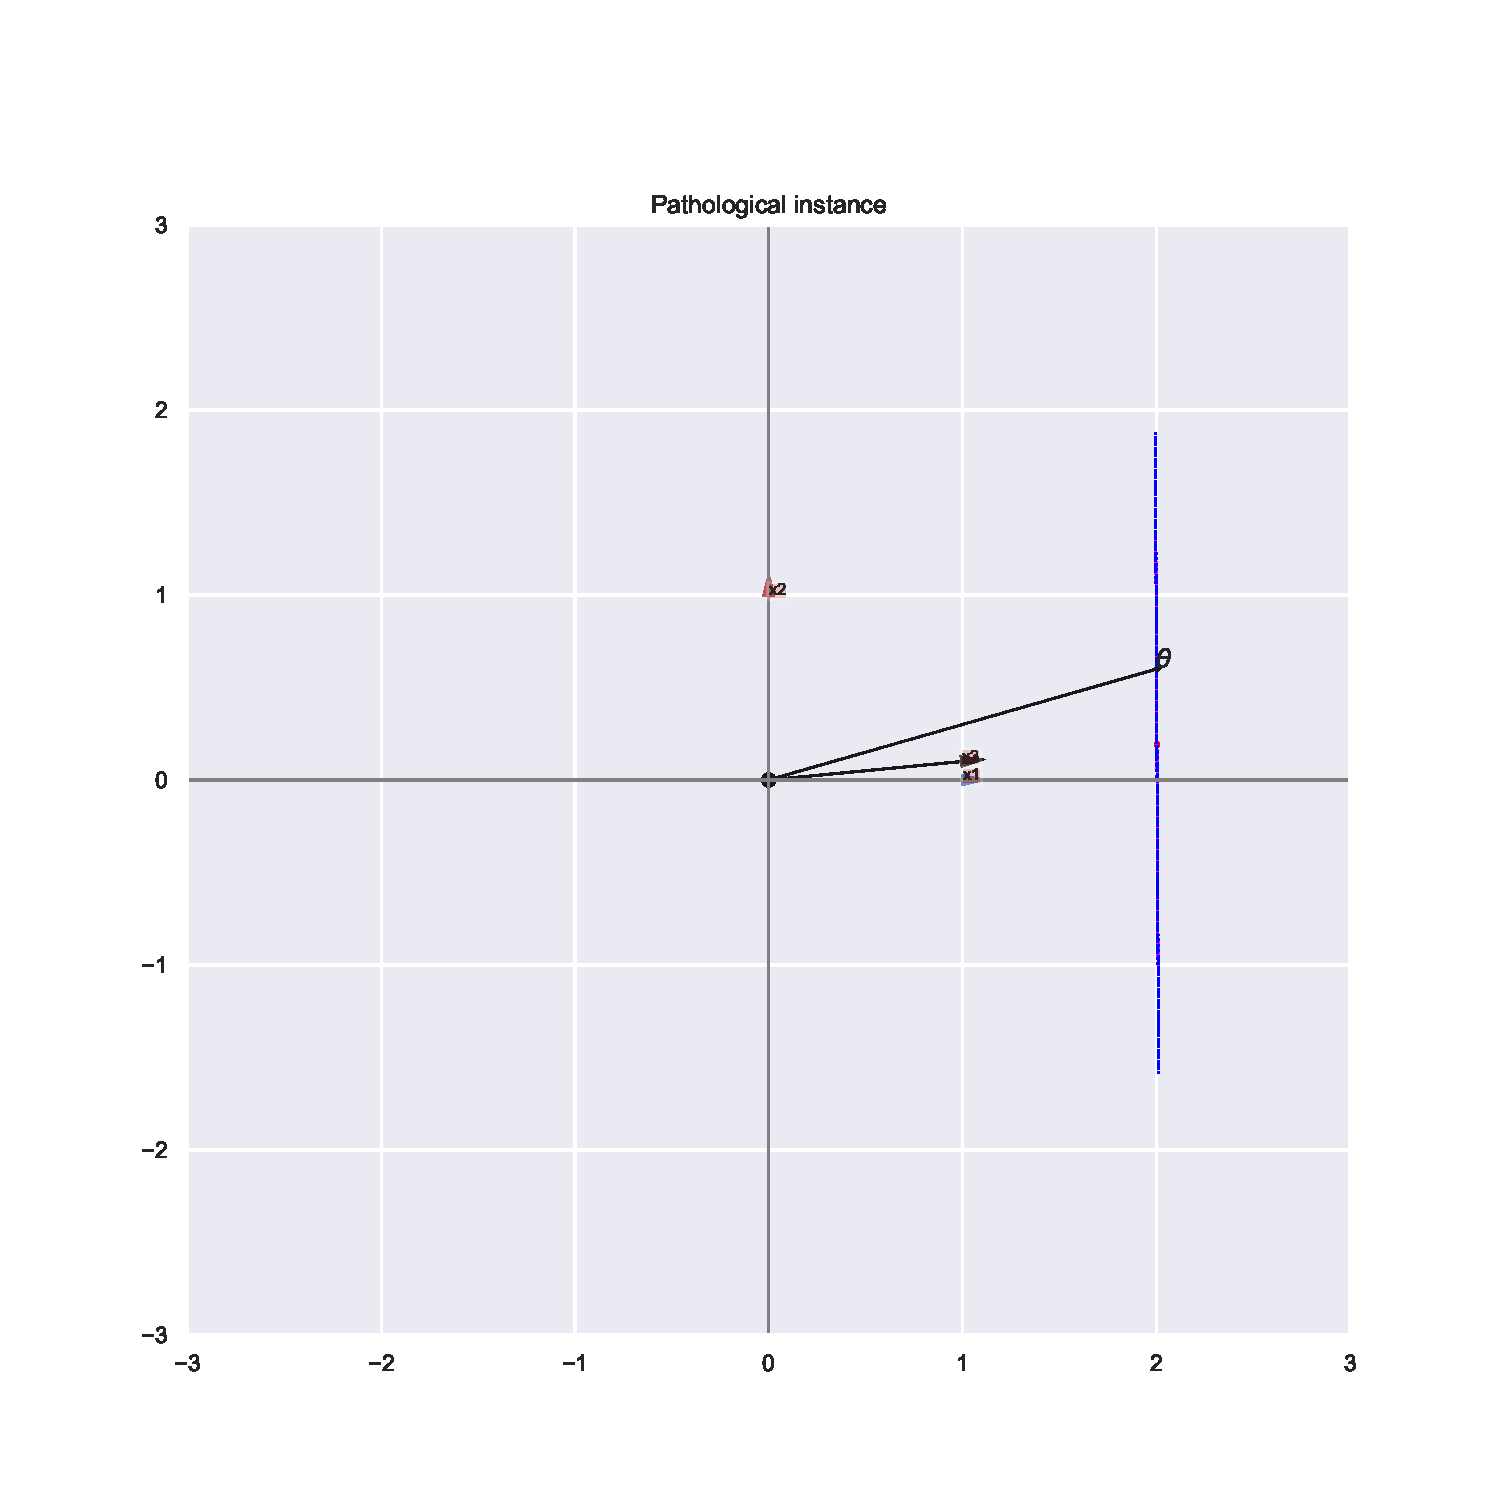
\includegraphics[width=0.55\textwidth]{Chapter4/img/instance.pdf}
    \caption{A pathological problem instance for linear best-arm identification.}
    \label{fig:instance}
\end{figure}

\subsection{A "greedy" fix of \LTCC{}}\label{sec:lgc.bayesian.fix}

A potential fix of the previous issue is the greedy version of $\LTCC$ whose pseudo-code is displayed in Algorithm~\ref{alg:lt3cg}. It is inspired by the \emph{greedy} rule already used in (a heuristic version of) \LGapE~\citep{xu2018linear}, and is motivated by the following observation: in order to learn to discriminate between some arm $I^{(1)}$ and a challenger $I^{(2)}$, it may be more informative to select another arm. More specifically, the arm from which a new pull would reduce the most the variance in the estimation of $\bx_{I^{(1)}} - \bx_{I^{(2)}}$. In a standard bandit, this is simply the least pulled arm between $I^{(1)}$ and $I^{(2)}$, but in the linear case it may be another arm!

\begin{algorithm}[ht]
\centering
\caption{Sampling rule of \LTCCG{}}
\label{alg:lt3cg}
%\footnotesize
\begin{algorithmic}[1]
    %(and the $W_n$ function for \textcolor{red}{\TCC})
   %\STATE {\bfseries Initialization:} $\forall \blambda\in\Omega, S_{\blambda}=0, F_{\blambda}=0$
   \For{$n \leftarrow 1,2,\cdots$}
        \State \text{Sample} $\btheta_1 \sim \Pi_n$
        \State $\hat{\bx}^{(1)} \leftarrow \argmax_{\bx\in\cX} \bx\transpose\btheta_1$ \text{(indexed by $I^{(1)}$)}
	        \State $I^{(2)} \leftarrow \argmin_{i\neq I^{(1)}}W_n(I^{(1)},i)$ \text{(see \eqref{def:transportation} for the definition)}\Comment{$I^{(2)} \leftarrow \hat{\bx}^{(2)}$}
		    \State \text{Evaluate arm} $\hat{\bx} \eqdef \argmin_{\bx\in\cX} \normm{\hat{\bx}^{(1)} - \hat{\bx}^{(2)}}_{(\bA_{\bX_n}+\bx\bx\transpose)^{-1}}$
	    \State \text{Update mean and variance according to \eqref{eq:update_mean} and \eqref{eq:update_variance}}
	    \State $n = n+1$
   \EndFor
\end{algorithmic}
\end{algorithm}

\subsection{\texorpdfstring{\LGapE}{} versus \texorpdfstring{\LTCCG}{}: Is one of them optimal?}\label{sec:lgc.bayesian.check}

Upon close examination, \LGapE and \LTCCG are very similar: they both rely on the computation of a leader and a challenger followed by the greedy rule to decide which arm to explore/play, and they actually use the same stopping rule (up to possible tuning of the threshold). The differences are:
\begin{itemize}
    \item how they define the challenger once the leader is chosen;
    \item how they perform exploration: \LGapE{} performs exploration in the choice of the challenger, which depends on some confidence bounds. \LTCCG{} performs exploration in the choice of the leader, which is determined by Thompson sampling.  
\end{itemize}

Table~\ref{tab:comparison} provides a more detailed comparison of the two algorithms for linear bandits. We see in particular that the stopping rule coincide up to the choice $C_n = \sqrt{2d_{n,\delta}}$.

\begin{table}[ht]
\centering
    %\hspace{-1cm}
    \resizebox{\textwidth}{!}{%
    \begin{tabular}{|c|c|c|}
    \hline 
      &  \LGapE & \LTCCG  \\
      \hline 
      Leader & $I_n^{(1)} = \argmax_{i}\bx_i\transpose\hat{\btheta}_n^{\lambda}$   &   $I_n^{(1)} = \argmax_{i} \bx_i\transpose\tilde{\btheta}_n$ \\
      & with $\hat \btheta_n^{\lambda}$ the least square estimate & with $\tilde{\btheta}_n \sim \mathcal{N}(\hat \btheta_n^\lambda,\hat{\bSigma}_n)$ \\
      \hline
        Challenger & $I_n^{(2)} = \underset{j \neq I_n^{(1)} }{\argmax} \ \left(\bx_j - \bx_{I_n^{(1)}}\right)\transpose \hat{\btheta}_n^\lambda + \normm{\bx_j - \bx_{I_n^{(1)}}}_{\hat{\bSigma}_n} C_n$    &   $I_n^{(2)} = \underset{j \neq I_n^{(1)} }{\argmin} \ddfrac{\left( \left(\bx_j - \bx_{I_n^{(1)}}\right)\transpose \hat\btheta_n^\lambda\right)^2}{2\normm{\bx_j - \bx_{I_n^{(1)}}}_{\hat{\bSigma}_n}^2} \1\left\{\bx_{I_n^{(1)}}\transpose\hat\btheta_n^\lambda \geq \bx_{j}\transpose\hat\btheta_n^\lambda\right\}$ \\
      \hline
          Stopping & $ \left(\bx_{I_n^{(2)}} - \bx_{I_n^{(1)}}\right)\transpose \hat\btheta_n^\lambda + \normm{\bx_{I_n^{(2)}} - \bx_{I_n^{(1)}}}_{\hat\bSigma_n} C_n < 0$    &  $\underset{j \neq J_n^{(1)} }{\min} \ddfrac{\left( \left(\bx_j - \bx_{J_n^{(1)}}\right)\transpose \hat\btheta_n^\lambda\right)^2}{2\normm{\bx_j - \bx_{J_n^{(1)}}}_{\hat{\bSigma}_n}^2} \1\left\{\bx_{J_n^{(1)}}\transpose\hat\btheta_n^\lambda \geq \bx_{j}\transpose\hat\btheta_n^\lambda\right\} > d_{n,\delta}$ \\
                 & $ \Leftrightarrow \ddfrac{\left(\left(\bx_{I_n^{(1)}} - \bx_{I_n^{(2)}}\right)\transpose \hat\btheta_n^\lambda\right)^2}{2\normm{\bx_{I_n^{(2)}} - \bx_{I_n^{(1)}}}_{\hat\bSigma_n}^2} > C_n^2/2$    &   $\Leftrightarrow J_n^{(1)} = \argmax_{j} \bx_j\transpose\hat{\btheta}_n^\lambda, \ \ddfrac{\left(\left(\bx_{J_n^{(1)}} - \bx_{J_n^{(2)}}\right)\transpose \hat\btheta_n^\lambda\right)^2}{2\normm{\bx_{J_n^{(2)}} - \bx_{J_n^{(1)}}}_{\hat\bSigma_n}^2} > d_{n,\delta}$ \\
          \hline
    \end{tabular}%
    }
\caption{Comparison between the two algorithms.} \label{tab:comparison}
\end{table}

\paragraph{Experiments for classical bandits.}
\LTCCG can be particularized to the classic BAI setting (that corresponds to choosing the canonical basis as contexts). In that case, the selection rule in Line 6 of Algorithm~\ref{alg:lt3cg} corresponds to choosing the least pulled arm between the two candidates. 

We investigate whether \LTCCG{} could be optimal in the classical bandit setting with some experiments. In particular, we call the derived algorithm \TCCG{}. See Fig.~\ref{fig:convergence} for a comparison against the asymptotically optimal \DT rule and the oracle. It is seemingly that \LTCCG{} is not very promising for being asymptotically optimal.

\begin{figure}[ht]
    \centering
    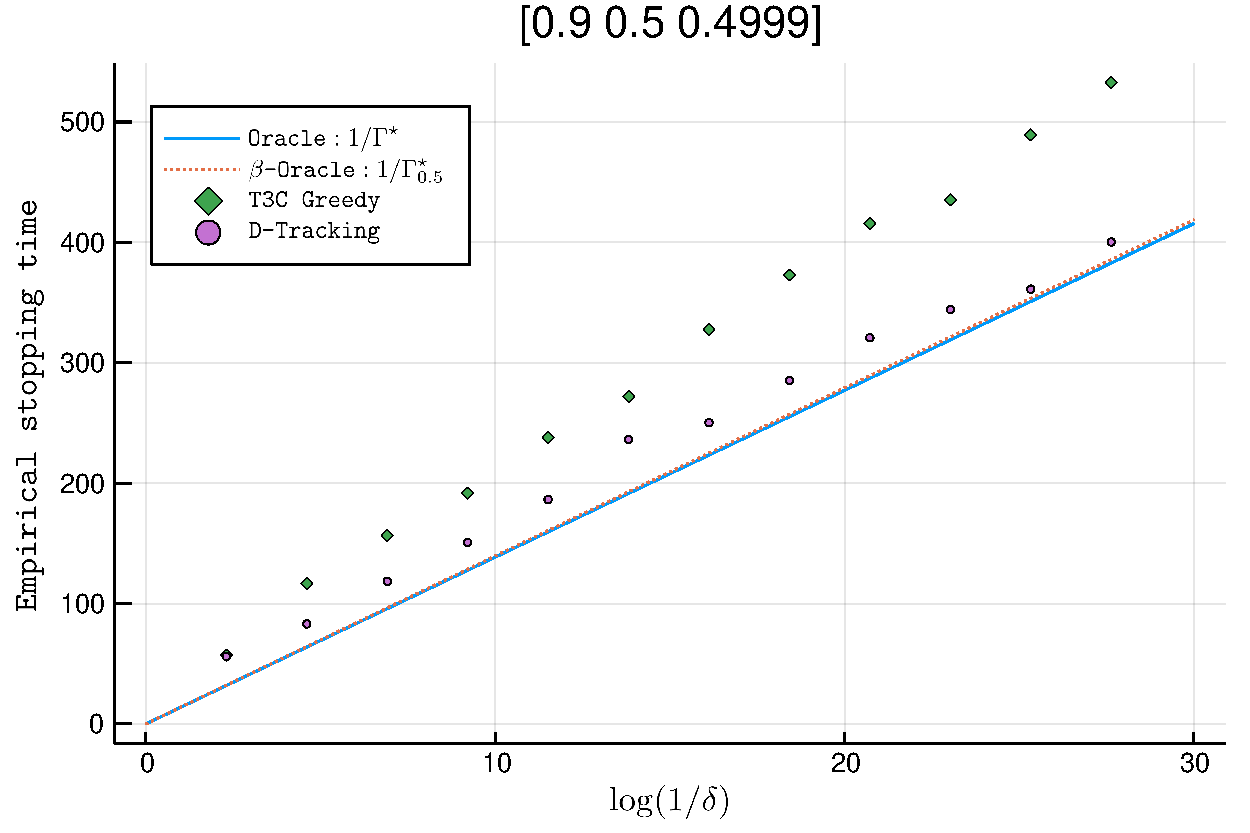
\includegraphics[width=0.33\textwidth]{Chapter4/img/res1.pdf}
    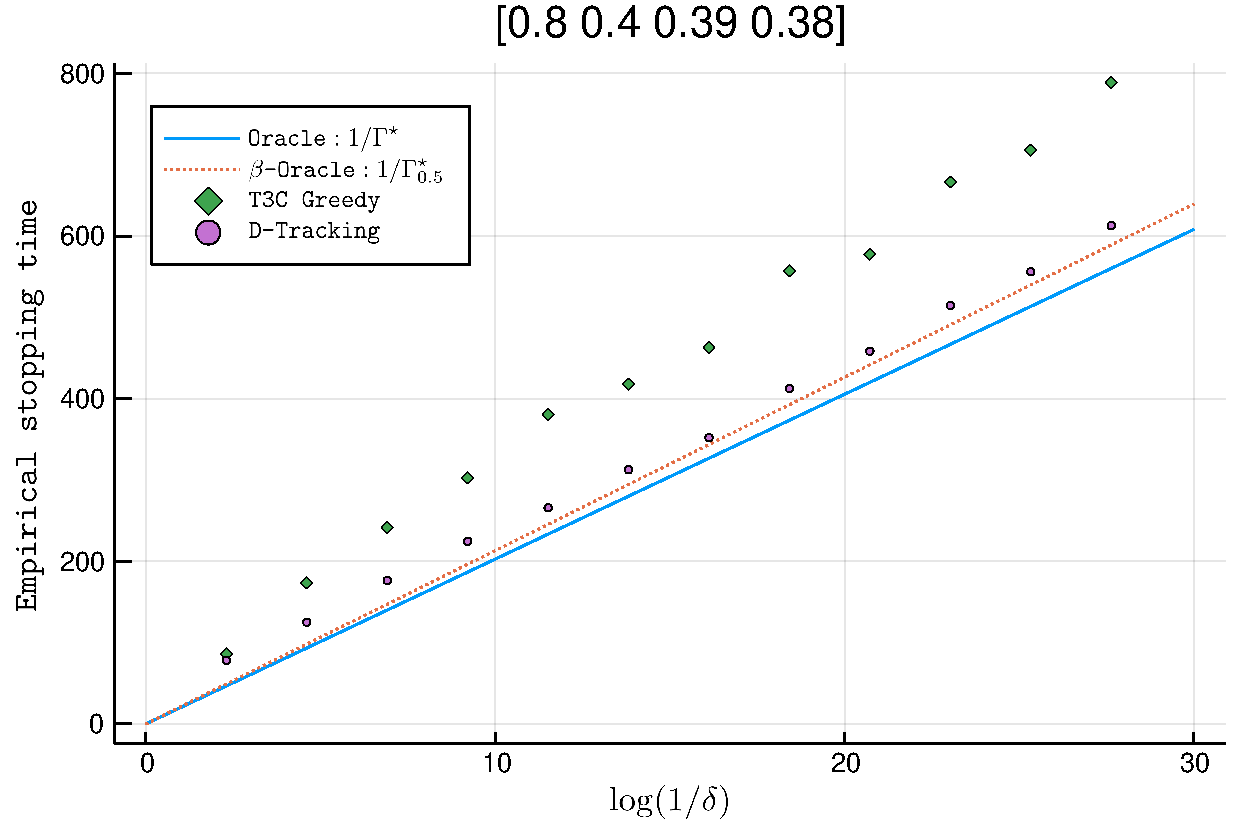
\includegraphics[width=0.33\textwidth]{Chapter4/img/res2.pdf}
    \caption{\TCCG{} versus \Track{} for different value of $\delta$.}
    \label{fig:convergence}
\end{figure}

\subsection{Empirical performance of \LTCCG{}}

\paragraph{The usual hard instance.}
We compare the performance of \LTCCG{} to \LGapE{} over the aforementioned hard instance with $d=2$, $c=2$ and two values of $\alpha$. More precisely, we report in Table~\ref{table:pulls1} the total number of pulls and also the number of pulls allocated to each arm for each of the sampling rules. The results confirm our intuition in the previous section. 

\begin{table}[ht]
\centering
\begin{tabular}{|c|c|c|}
 \hline
 & \LTCCG & \LGapE \\
 \hline
 \textbf{$\bx_1=(1,0)\transpose$} & $1783.1$ & $5844.4$ \\
 \hline
 \textbf{$\bx_2=(0,1)\transpose$} & $357009.0$ & $1169260.5$ \\
 \hline
 \textbf{$\bx_3=(\cos(0.01),\sin(0.01)\transpose)$} & $1.0$ & $1.0$ \\
 \hline
 \textbf{Total} & $\textbf{358793.1}$ & $1175105.9$ \\
 \hline
\end{tabular}
\caption{Average number of pulls of each arm ($d=2, \delta=0.1$).}
\label{table:pulls1}
\end{table}

\begin{table}[ht]
\centering
\begin{tabular}{|c|c|c|c|}
 \hline
 & \LTCC ($\beta=1/2$) & \LTCCG & \LGapE \\
 \hline
 \textbf{$\bx_1=(1,0)\transpose$} & $131.3$ & $24.9$ & $26.3$ \\
 \hline
 \textbf{$\bx_2=(0,1)\transpose$} & $3.3$ & $60.8$ & $63.4$ \\
 \hline
 \textbf{$\bx_3=(\cos(\pi/4),\sin(\pi/4)\transpose)$} & $133.4$ & $1.0$ & $1.0$ \\
 \hline
 \textbf{Total} & $268.0$ & $\textbf{86.7}$ & $89.7$ \\
 \hline
\end{tabular}
\caption{Average number of pulls of each arm ($d=2, \delta=0.1$).}
\label{table:pulls2}
\end{table}

\paragraph{Arms with mild gaps.}
We can also provide more experimental illustrations on different types of problem.

We construct a set of $K$ arms proposed by~\cite{fiez2019transductive}:
\[
    \bx_1=(1,0)\transpose, \bx_2=(\cos(3\pi/4),\sin(3\pi/4))\transpose\,,
\]
and for $k = 3,\ldots,K$, 
\[
    \bx_k=(\sin(\pi/4+\phi_k),\cos(\pi/4+\phi_k))\transpose
\]
where $\phi_i\sim\cN(0,0.09)$. We fix the true regression parameter $\theta$ to be $\be_1$. This set of arms has some nice properties, that $\bx_1$ is the optimal arm, and $\bx_2$ is the arm that gives more information on identifying the best arm. We first report results with a moderate $K=6$ as an example where the generated expected means are $[1.0, -0.71, 0.84, -0.95, 0.93, 0.99]$.

\begin{table*}[ht]
\centering
\def\arraystretch{1.2}
\begin{tabular}{|c|c|c|c|}
 \hline
 & \LTCC & \LTCCG & \LGapE \\
 \hline
 \textbf{$\bx_1=(1,0)\transpose$} & $170872.19$ & $1.06$ & $1.13$ \\
 \hline
 \textbf{$\bx_2=(\cos(3\pi/4),\sin(3\pi/4))\transpose$} & $1.25$ & $1.0$ & $1.0$ \\
 \hline
 \textbf{$\bx_3=(\sin(\pi/4+\phi_3),\cos(\pi/4+\phi_3))\transpose$} & $92.18$ & $28693.26$ & $120657.6$ \\
 \hline
 \textbf{$\bx_4=(\sin(\pi/4+\phi_4),\cos(\pi/4+\phi_4))\transpose$} & $1.12$ & $26197.03$ & $110157.63$ \\
 \hline
 \textbf{$\bx_5=(\sin(\pi/4+\phi_5),\cos(\pi/4+\phi_5))\transpose$} & $77.04$ & $1.0$ & $1.0$ \\
 \hline
 \textbf{$\bx_6=(\sin(\pi/4+\phi_6),\cos(\pi/4+\phi_6))\transpose$} & $170892.82$ & $1.36$ & $1.83$ \\
 \hline
 \textbf{Total} & $341936.6$ & $\textbf{54894.71}$ & $230820.19$ \\
 \hline
\end{tabular}
\caption{average number of pulls of each arm ($d=2, \delta=0.1$).}
\label{table:pulls3}
\end{table*}

\paragraph{Impact of the dimension.}
We also compare the impact of the dimension $d$ over the performance of our sampling rule and $\LGapE$. We run experiments on the same instance with a value of the angle set to $\alpha=0.1$. This time we let the dimension $d$ varying from 2 to 6. \LTCC{} is always better and the performance gap increases with the dimension. Thus, our algorithm seems to be more robust to the dimension.

\begin{figure}[ht]
    \centering
    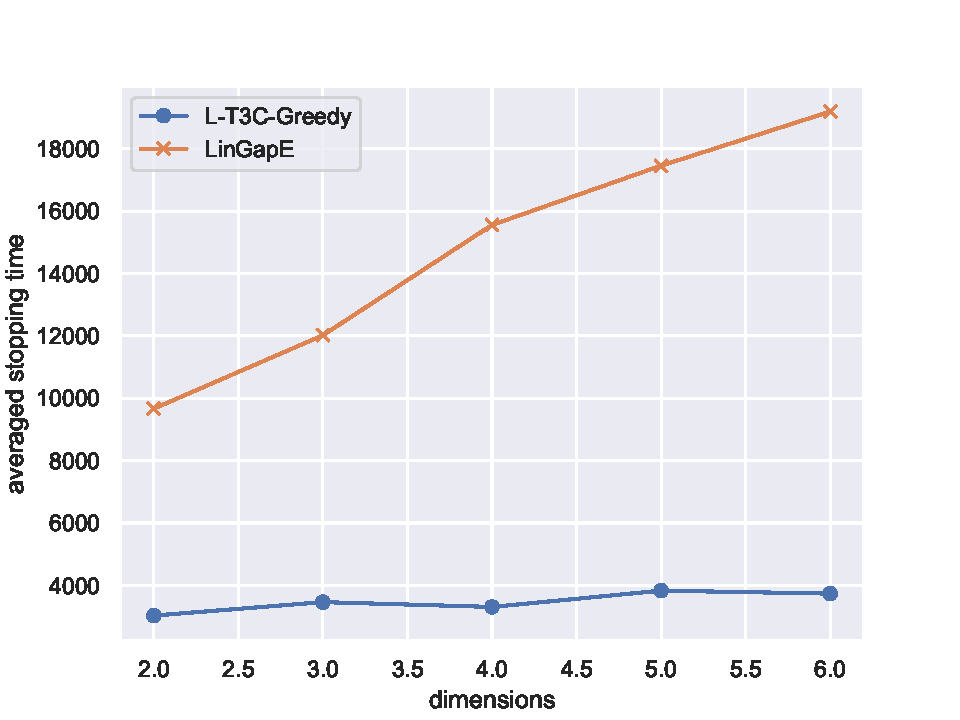
\includegraphics[width=0.5\textwidth]{Chapter4/img/dims.pdf}
    \caption{Comparison of the sample complexity of \LTCCG{} and \LGapE{} on the pathological instance in $\R^d$ for different values of $d$.}
    \label{fig:dims}
\end{figure}

\paragraph{Rank-1 multivariate normal distribution sampling.}
A technical point for the experiments in this section is to sample from a multivariate normal distribution (e.g. for \LTCC{}). We can proceed by the following.

Indeed, a random Gaussian vector 
\[
    \bX = (X_1, X_2, \ldots, X_d)\transpose
\] 
of mean vector $\bar{\bmu}$ and covariance matrix $\bSigma$ can be formally defined as following,
\[
    \bX \sim \cN(\bar{\bmu}, \bSigma) \iff \exists \bar{\bmu}\in\mathbb{R}^d,\bA\in\mathbb{R}^{d\times d'} \ \text{s.t.} \ \bX = \bA \mathbf{Z} + \bar{\bmu},
\]
for $Z_i \sim\ \mathcal{N}(0, 1)$ i.i.d. with $i\in\{1,\ldots,d'\}$, and here $\bSigma = \bA\bA\transpose$.

To draw a sample from a multivariate normal distribution, according to the previous definition, one can first find any real matrix $\bA$ such that $\bA\bA\transpose = \bSigma$. Then draw a vector $\bZ$ whose components independently follow standard normal distribution. Finally $\bX = \bA \mathbf{Z} + \bar{\bmu}$ forms a valid sample. The main issue is thus how to find an appropriate matrix $\bA$.

In this section, we need to sample from $\cN(\hat{\btheta}^\lambda_n,\hat{\bSigma}_n)$, where the covariance matrix $\hat{\bSigma}_n$ is a positive-definite matrix. A usual way is to apply the Cholesky decomposition, which is computationally inefficient if it were to be applied at each time step. Fortunately, we can apply rank-1 Cholesky decomposition in our case.  

%We, however, notice that $\bA = (\hat{\bSigma}_n)^{1/2}=\sigma(\bB^{\lambda}_n)^{-1/2}$ is also a valid candidate, and is thus can be also updated iteratively using a similar formula to the Sherman-Morrison formula.

%More precisely, we have
%\begin{align*}
%    \forall t\geq 0, \quad (\bB^{\lambda}_{t+1})^{-\frac{1}{2}} = (\bB^{\lambda}_t)^{-\frac{1}{2}} - \ddfrac{\left(1-\sqrt{1-\frac{\normm{\hat{\bx}_{t+1}}_{(\bB^{\lambda}_t)^{-1}}^2}{1+\normm{\hat{\bx}_{t+1}}_{(\bB^{\lambda}_t)^{-1}}^2}}\right)}{\normm{\hat{\bx}_{t+1}}_{(\bB^{\lambda}_t)^{-1}}^2} (\bB^{\lambda}_t)^{-\frac{1}{2}}\hat{\bx}_{t+1}\hat{\bx}_{t+1}\transpose(\bB^{\lambda}_t)^{-\frac{1}{2}}.
%\end{align*}

% \subsection{Technical tools}

% \subsection{Tail bounds}
% Following are the classic Gaussian tail bound inequalities written in our linear context (see e.g.~\citealt{qin2017ttei} for detailed proofs).

% \begin{lemma}\label{lemma:tail_upper}
% For any $i,j\in\{1,\ldots,K\}$, if $\bx_i\transpose\hat{\btheta}^\lambda_n<\bx_j\transpose\hat{\btheta}^\lambda_n$,
% \begin{align}
%     \Pi_n\left[\bx_i\transpose\btheta>\bx_j\transpose\btheta\right] &\leq \frac{1}{2} \expp{-\frac{\left(\bx_j\transpose\hat{\btheta}^\lambda_n-\bx_i\transpose\hat{\btheta}^\lambda_n \right)^2}{2\normm{\bx_i-\bx_j}_{\hat{\bSigma}_n}^2}}.
% \end{align}
% \end{lemma}

% \begin{lemma}\label{lemma:tail_lower}
% For any $i,j\in\{1,\ldots,K\}$, if $\bx_i\transpose\hat{\btheta}^\lambda_n<\bx_j\transpose\hat{\btheta}^\lambda_n$,
% \begin{align}
%     \Pi_n\left[\bx_i\transpose\btheta>\bx_j\transpose\btheta\right] &\geq \frac{1}{\sqrt{2\pi}} \expp{-\frac{\left(\bx_j\transpose\hat{\btheta}^\lambda_n-\bx_i\transpose\hat{\btheta}^\lambda_n +\normm{\bx_i-\bx_j}_{\hat{\bSigma}_n}\right)^2}{2\normm{\bx_i-\bx_j}_{\hat{\bSigma}_n}^2}}.
% \end{align}
% \end{lemma}


%!TEX root = ../Chapter4.tex
\section{A Gamified Algorithm}\label{sec:lgc.game}

The first attempt using Bayesian machinery does not end up with a satisfying output. In this section, we turn our thoughts to another idea and take inspiration from the \emph{zero-sum game} (see e.g.~\citealt{degenne2019pure}). We describe \LG{}, detailed in Algorithm~\ref{alg:lg}. As noted in the seminal work of \citet{chernoff1959}, the complexity $\Tstar(\btheta)^{-1}$ is the value of a fictitious zero-sum game between the learner choosing an optimal proportion of allocation of pulls $\bomega$ and a second player, the nature, that tries to fool the agent by responding with the most confusing alternative $\btheta'$ leading to an incorrect answer. \LG{} is an asymptotically optimal algorithm for linear bandits BAI. Note that the present algorithm is asymptotically optimal for the general pure exploration game, which is however not the main focus of this thesis. Lecturers can refer to~\cite{degenne2020game} for more details.

In this section, we make the following extra assumption.
\begin{assumption}\label{ass:lgc.bounded_parameter}
\begin{leftbar}[assumptionbar]
We assume that $\exists M>0$, s.t. $\forall \btheta\in\Theta$, $\normm{\btheta} \leq M$, where $\normm{\btheta}$ denotes the Euclidean norm of the vector $\btheta$. 
\end{leftbar}
\end{assumption}

%The full analysis of the algorithm is omitted as well as a convexified version \LGC{} -- also asymptotically optimal itself -- as they are not the main focus of this thesis. Lecturers can refer to~\cite{degenne2020game} for the complete proofs.


% , i.e for $i\in\cI$ and $w\in\interior{\Sigma_A}$ in the interior of the probability simplex of dimension $A-1$, find $\lambda^i$ such that
% \[
% \lambda^i \in \argmin_{\lambda\neg i}\normm{\theta - \lambda }_{V_{w}}\,.
% \]


%Note that in the proof of Theorem~\ref{thm:sample_complexity} we only use two times the boundedness assumption, first in the definition of the threshold $\beta(t,\delta)$ (see Theorem~\ref{th:confidence_beta}) to handle the bias induced by the regularization. Second, since the regret of AdaHedge is proportional to the maximum of the upper confidence bounds $U_s^{i,a}$, we need to ensure that they are bounded.

% And there exists pathological pure exploration problems where even the quantity uppper bounded by $U_s^{i,a}$, namely $\normm{\theta-\lambda}_{aa^\top}^2$ where $\lambda\in\argmin_{\lambda'\in\neg i}\normm{\theta -\lambda}$ is unbounded\todo{I don't understand what this means.}. See for example Appendix~G.3 by \citet{menard2019lma}.

\subsection{Notations}

In this section, besides the usual learner, we include an extra fictive player -- the nature -- and we thus introduce some specific notation of counts for this section.

At each round $n$ the algorithm to be presented will play an arm $\hbx_n$ and choose (fictitiously) an answer $i_n\in\cI$. We denote by $N_n^{\bx,i} \eqdef\sum_{t=1}^n \ind_{\{(\hbx_n,i_n)=(\bx,i)\}}$ the number of times the pair $(\bx,i)\in\cX\times\cI$ is chosen up to and including time $n$, and by $N_n^\bx =\sum_{i\in\cI} N_n^{\bx,i}$ and $N_n^i =\sum_{\bx\in\cX} N_n^{\bx,i}$ the partial sums. The vectors of counts at time $n$ is denoted by $\bN_n \eqdef (N_n^\bx)_{\bx\in\cX}$
and when it is clear from the context we will also denote by $\bN_n^{\bx} = (N_n^{\bx,i})_{i\in\cI}$ and $\bN_n^i = (N_n^{\bx,i})_{\bx\in\cX}$ the vectors of partial counts. Remind that in the case of BAI, $\cX=\cI$.

%\paragraph{Regularized least square estimator.} We fix a regularization parameter $\eta > 0$. The regularized least square estimator for the parameter $\theta\in \mathcal M$ at time $t$ is
%\[
%\htheta_{t} = (V_{N_t} + \eta I_d)^{-1} \sum_{s=1}^t Y_s a_s\,,
%\]
%where $I_d$ is the identity matrix. By convention $\htheta_0 = 0$.


\subsection{The \LG{} algorithm}

The pseudo-code of \LG{} is provided in Algorithm~\ref{alg:lg}. We interpret each component of the algorithm by next.

\begin{algorithm}[ht]
\centering
\caption{Algorithm of \LG{}}
\label{alg:lg}
\begin{algorithmic}[1]
    \State {\bfseries Input:} Learners for each answer $(\cL^i_\bomega)_{i\in\cI}$, threshold $d$
    \For{n = 1 \ldots}
        \State \textit{// Stopping rule}
        \If{{$\max_{i\in\cI}\inf_{\btheta'\in\neg i} \frac{1}{2}\normm{\hbtheta_{n-1}^\lambda-\btheta'}^2_{\bLambda_{\bN_{n-1}}}\geq d_{n-1,\delta}$}}
            \State \text{Stop} 
            \State {\bfseries Return} $J_n = \Istar(\hbtheta_{n-1}^\lambda)$
        \EndIf
        \State \textit{// Empirical best guess}
        \State $i_n = \Istar(\hbtheta_{n-1}^\lambda)$
        \State \textit{// Learner plays first}
        \State \text{Get} $\bomega_n$ \text{from} $\cL^{i_n}_\bomega$
        \State \text{Update} $\bW_n=\bW_{n-1}+\bomega_n$
        \State \textit{// Best response of the nature}
        \State $\btheta_n^{i_n} \in \argmin_{\btheta'\in\neg i_n}\normm{\hbtheta_{n-1}^\lambda-\btheta'}^2_{\bLambda_{\bomega_n}}$
        \State \textit{// Feed optimistic gains}
        \State \text{Feed learner} $\cL_\bomega^{i_n}$ \texttt{with} $g_{n}(\bomega) = \sum_{\bx\in\cX}\omega_\bx U_n^{\bx,i_n}/2$
        \State \textit{// Track the weights}
        \State \text{Pull} $\hbx_n \in \argmin_{\bx\in \cX} N_{n-1}^{\bx} - W_{n,\bx}$
   \EndFor
\end{algorithmic}
\end{algorithm}

% \begin{algorithm}[tb]
% \centering
% \caption{\LGC}
% \label{alg:lgc}
% \begin{algorithmic}[1]
%     \State {\bfseries Input:} Agent learner $\cL_{\tw}$, threshold $\beta(\cdot,\delta)$
%     \For{t = 1 \ldots}
%         \State \textit{// Stopping rule}
%         \If{ {\small $\max_{i\in \cI} \inf_{\lambda\in\neg i} \frac{1}{2}\normm{\htheta_{t-1}-\lambda}^2_{V_{N_{t-1}}}\geq \beta(t-1,\delta)$}}
%             \State {\bfseries stop} and {\bfseries return} $\hi = \istar(\hat{\theta}_{t-1})$. 
%         \EndIf
%         \State \textit{// Agent plays first}
%         \State \texttt{get} $\tw_{t}$ \texttt{from} $\cL_{\tw}$ 
%         \State \texttt{update} $\tW_{t}=\tW_{t-1}+\tw_{t}$
%         \State \textit{// Best response for the nature}
%         \State $\forall i\in\cI$, $\tlambda^i_{t} \in \argmin_{\lambda\in\neg i}\normm{\htheta_{t-1}-\lambda}^2_{V_{\tw^i_{t}}}$
%         \State \textit{// Feed optimistic gains}
%         \State \texttt{feed learner} $\cL_{\tw}$ \texttt{with} {$g_{t}(\tw) =\sum_{(a,i)\in\cA\times\cI} \tw^{a,i} U_t^{a,i}/2$}
%         \State \textit{// Track the weights}
%         \State \texttt{pull} $(a_{t},i_{t})\in \argmin_{(a,i)\in \mathcal A \times \mathcal I} N_{t-1}^{a,i} - \tW_{t}^{a,i}$
%     \EndFor
% \end{algorithmic}
% \end{algorithm}

\paragraph{Stopping rule and decision rule.}
We follow the same stopping rule and decision rule of Section~\ref{sec:lgc.bayesian}\footnote{It is easy to check that~\eqref{eq:lgc.lg_stopping} and~\eqref{eq:lgc.lg_decision}) are equivalent to~\eqref{eq:lgc.bayesian_stopping} and~\eqref{eq:lgc.bayesian_decision} respectively.}: \LG{} stops if a generalized likelihood ratio exceeds a threshold $d_{n,\delta}$. With the notation of this section, the stopping time can be written as
\begin{align}\label{eq:lgc.lg_stopping}
    \max_{i\in \cI} \inf_{\btheta' \in \neg i}\frac{1}{2}\Vert \hbtheta_n^\lambda - \btheta' \Vert^2_{\bLambda_{\bN_n}} > d_{n,\delta}\,,
\end{align}
and the decision rule is 
\begin{align}\label{eq:lgc.lg_decision}
    J_n = \argmax_{i\in \cI} \inf_{\btheta' \in \neg i}\Vert \hbtheta_n^\lambda - \btheta' \Vert^2_{\bLambda_{\bN_n}}/2\,.
\end{align}

Similarly to \TCC{}/\TTTS{} of Chapter~\ref{CHAP:T3C}, these stopping and decision rules ensure that the \LG{} is $\delta$-correct regardless of the sampling rule used, see lemma below\footnote{The fact that $\tau_\delta <+\infty$ is a consequence of our analysis, see Appendix~\ref{app:lgc.proof}.} proved in Appendix~\ref{app:lgc.lemmas}.

\begin{lemma}\label{lemma:lgc.pac}
\begin{leftbar}[lemmabar]
Regardless of the sampling rule, the stopping rule~\eqref{eq:lgc.lg_stopping} with the threshold
\begin{equation} \label{eq:def_beta}
    d_{n,\delta} =\left( \sqrt{\log\left( \frac{1}{\delta}\right)+\frac{d}{2}\log\left(1+\frac{n L^2}{\lambda d} \right)} +\sqrt{\frac{\lambda}{2}}M\right)^2\,,
\end{equation}
satisfy
\[
    \PPt{\big(\tau_{\delta} < \infty \wedge J_\tau \neq \Istar(\btheta)\big)} \leq \delta\,.
\]
\end{leftbar}
\end{lemma}
% This stopping and decision rules ensures that the algorithm is $\delta$-correct regardless of the sampling rule used (see \citealt{garivier2016tracknstop} for a proof), hence the following theorem is immediate.
% \begin{theorem}
% Algorithms~\ref{alg:lg} and~\ref{alg:lgc} are $\delta$-correct.
% \end{theorem}
Our contribution is a sampling rule that minimizes the sample complexity when combined with these stopping and decision rules.
We now explain our sampling strategy to ensure that the stopping threshold is reached as soon as possible.

\paragraph{Saddle-point computation.}
Suppose in this paragraph, for simplicity, that the regression parameter $\btheta$ is known to the learner. By the definition of stopping rule and generalized likelihood ratio, as long as the algorithm does not stop, we have
\begin{align*}
    d_{n,\delta} \ge \inf_{\btheta'\in \neg \Istar(\btheta)} \sum_{\bx\in \cX} N_n^\bx \Vert \btheta - \btheta' \Vert^2_{\bx\bx\transpose}/2\,.
\end{align*}
Now, let $\bomega^\star(\btheta)$ be the optimal pulling proportions given $\btheta$. If we manage to have $\bN_n \approx n\bomega^\star(\btheta)$, then it follows $d_{n,\delta} \ge n T^\star(\btheta)^{-1}$ and, solving that equation would lead to the asymptotic optimality.

% Since there is only one correct answer, the parameter $\btheta$ belongs to all sets $\neg i$ for $i\neq \Istar(\btheta)$. Hence
% \begin{align*}
% &\inf_{\lambda\in \neg i^\star(\theta)}\frac{1}{2} \sum_{a\in \cA} N_t^a \Vert \theta - \lambda \Vert^2_{a a^\top}
% \\&\geq \inf_{\tlambda_t\in \prod_i (\neg i)}\frac{1}{2}\sum_{(a,i)\in \cA\times\cI}\!\!\!\!\! N_t^{a,i} \Vert \theta - \tlambda^i \Vert^2_{a a^\top}.
% \end{align*} Introducing the sum removes the dependence in the unknown $i^*(\theta)$. \LGC then uses an agent playing weights w in $\Sigma_{\cA\cI}$. 

At each time step, \LG{} produces a guess $i_n$ for $\Istar(\btheta)$ and its analysis involves proving that the guess is wrong only finitely-many times in expectation.

The sampling rule implements a lower-bound game between a learner, playing at each stage $n$ a pull-proportion/weight vector $\bomega_n$ in the probability simplex $\Sigma_K$, and nature, who computes at each stage a response $\btheta_n \in \neg i_n$. We additionally ensure that $N_n^\bx \approx \sum_{t=1}^n \omega_{t,\bx}$, where $\omega_{n,\bx}$ denotes the weight of $\bx$ at stage $n$. The goal of the sampling rule is to ensure a $\epsilon$-approximation of the saddle point of the lower-bound game.

% Suppose that the sampling rule is such that at stage $t$, a $\varepsilon_t$-approximate saddle point is reached for the lower-bound game, see Lemma~\ref{lem:sion_convexify}. That is,
% \begin{align*}
% &\inf_{\tlambda \in \prod_{i}(\neg i)} \sum_{s=1}^t \sum_{(a,i)\in \cA\times\cI} \tw_s^{i,a} \Vert \theta - \tlambda^i \Vert^2_{a a^\top}/2 +\varepsilon_t
% \\
% &\ge \sum_{s=1}^t \sum_{(a,i)\in \cA\times\cI} \tw_s^{i,a} \Vert \theta - \tlambda_s^i \Vert^2_{a a^\top}/2
% \\
% &\ge\max_{(a,i)\in \cA\times\cI} \sum_{s=1}^t \Vert \theta - \tlambda_s^i \Vert^2_{a a^\top}/2 - \varepsilon_t \: .
% \end{align*}
% Then if the algorithm did not stop, it verifies, using Lemma~\ref{lem:sion_convexify},
% \begin{align*}
% \beta(t,\delta)
% &\ge t \max_{(a,i)\in \cA\times\cI} \frac{1}{t}\sum_{s=1}^t \Vert \theta - \tlambda_s^i \Vert^2_{a a^\top}/2 - 2\varepsilon_t
% \\
% &\ge t \inf_{\tq \in \mathcal \prod_{i\in \mathcal I}\cP(\neg i)} \! \max_{(a,i)\in \cA\times\cI} \!\!\!\! \mathbb{E}_{\lambda^i\sim q^i}\Vert \theta \! - \! \tlambda^i \Vert^2_{a a^\top}/2 \! - \! 2\varepsilon_t\\
% &= t T^\star(\theta)^{-1} - 2 \varepsilon_t \: .
% \end{align*}
% Solving that equation, we get asymptotically the wanted $t\lesssim T^\star(\theta) \log(1/\delta)$.

To achieve that, we implement the saddle-point algorithm by using \AH for the learner -- a regret-minimizing algorithm of the exponential family -- and using best-response for the nature, which plays after the agent. Precisely \LG{} uses $|\cI|$ ($=K$ for BAI) learners $\cL_\bomega^i$, one for each possible guess of $\Istar(\btheta)$ with the gains. For $i\in\cI$, the learner $\cL_\bomega^i$ is an \AH on the probability simplex $\Sigma_K$ with the gains (when the guess is $i$)
\[
    g_n^\btheta(\bomega) = \frac{1}{2} \sum_{\bx\in\cX}  \omega_{\bx} \Vert \btheta - \btheta_n^i \Vert^2_{\bx \bx\transpose}\,.
\]
$\epsilon$ is then the sum of the regrets of the two players. Best-response has regret 0, while the regret of \AH is $O(\sqrt{n})$ for bounded gains, as seen in the following lemma, taken from~\citet{derooij2014hedge}.

\begin{lemma}\label{lemma:lgc.adahedge}
\begin{leftbar}[lemmabar]
On the online learning problem with $K$ arms and gains $g_t(\bomega) = \sum_{k\in[K]} \omega_k  U_t^k$ for $t\in[n]$, \AH, predicting $(\bomega_t)_{t\in[n]}$, has regret
\begin{align*}
%R_T &\le 2\sqrt{(\sigma L_T - \frac{L_T^2}{T})\log(K)} + \sigma(2+\log(K)16/3) \: ,\\
    R_n &\eqdef \max_{\bomega\in\Sigma_K}\sum_{t=1}^n g_t(\bomega) - g_t(\bomega_t) \\
    &\le 2\eta\sqrt{n\log(K)} + 16\eta(2+\log(K)/3) \,,
%L_T &= \sum_{t=1}^T (\max_{k\in[K]}U_t^{k} - U_t^{\star}) \le T \sigma \: .
\end{align*}
where $\eta = \max_{t\le n}  (\max_{k\in[K]}U_t^{k}- \min_{k\in[K]}U_t^{k})$.
\end{leftbar}
\end{lemma}
Other combinations of learners are possible, as long as the sum of their regrets is sufficiently small. At each stage $n\in\NN$, both learners advance only by one iteration and as time progresses, the quality of the saddle-point approximation improves. This is in contrast with \CT and \DT of~\cite{garivier2016tracknstop}, in which an exact saddle point is computed at each stage, at a potentially much greater computational cost.

\paragraph{Optimism.} The above saddle-point argument would be correct for a known game, while our algorithm is confronted to a game depending on the unknown parameter $\btheta$. Following a long tradition of stochastic bandit algorithms, we use the principle of OFU. Given an estimate $\hbtheta_{n-1}$, we compute upper bounds for the gain of the real learner at $\btheta$, and feed these optimistic gains to them. Precisely, given the best response $\btheta_n^i \in \neg i$, we define,
\begin{align*}
    U_n^{\bx,i} =\left\{
    \begin{array}{ll}
    \max_{\xi} & \min\big(\Vert \bxi - \btheta_n^i \Vert^2_{\bx\bx\transpose},4L^2M^2\big)\\
    \text{s.t.} & \Vert \hbtheta_{n-1}^\lambda - \bxi \Vert^2_{\bLambda_{\bN_{n-1}}+\lambda I_d} \le 2h(n)
    \end{array}
    \right.\,,
\end{align*}
where $h(n)=\beta(n, 1/n^3)$ is some exploration function. 

We clipped the values, using Assumption~\ref{ass:lgc.bounded_arm} and Assumption~\ref{ass:lgc.bounded_parameter} to ensure bounded gains for the learners (see Section~\ref{sec:lgc.complexity.examples} for description of bounded BAI). 

Under the event that the true parameter verifies $\Vert \hbtheta_{n-1}^\lambda - \btheta \Vert^2 \le 2 h(n)$, this is indeed an optimistic estimate of $\Vert \btheta - \btheta_n^i \Vert^2_{\bx\bx\transpose}$. Note that $U_n^{\bx,i}$ has a closed form expression, see Appendix~\ref{app:lgc.proof}. The optimistic gain is then
\[
    g_{n}(\bomega) = \frac{1}{2}\sum_{\bx\in\cX}\omega_\bx U_n^{\bx,i_n}\,.
\]


\paragraph{Tracking.} In Algorithm~\ref{alg:lg}, the learner plays weight vectors in a simplex. Since the bandit procedure allows only to pull one arm at each stage, our algorithm needs a procedure to transcribe weights into pulls. This is what we call tracking, following~\citet{garivier2016tracknstop}. The choice of arm (or arm and answer) is
\begin{align*}
    \hbx_{n+1} \in \argmin_{\bx\in \cX } N_{n}^{\bx} - W_{n+1,\bx}\,.
\end{align*}
This procedure guarantees that for all $n\in\NN, \bx\in\cX$, we have $- \log (|\cX|) \le N_n^{\bx} - W_{n,\bx} \le 1$. This result is due to~\citet{degenne2020structure}.

\begin{theorem}\label{thm:lgc.sample_complexity}
\begin{leftbar}[theorembar]
For a regularization parameter\footnote{This condition is a simple technical trick to simplify the analysis. An $\lambda$ independent of $K$,$L$,$M$ will lead to the same results up to minor adaptations of the proof.} $\lambda \geq 2(1+\log(K))KL^2+M^2$, for the threshold $d_{n,\delta}$ given by~\eqref{eq:def_beta}, for an exploration function $h(n)=d_{n,1/n^3}$, \LG{} is $\delta$-correct and asymptotically optimal. That is, it verifies for all $\btheta\in \Theta$,
\begin{align*}
    \limsup_{\delta\to 0}\frac{\mathbb{E}_\btheta[\tau_\delta]}{ \log 1/\delta} \le \Tstar(\btheta) \,.
\end{align*}
\end{leftbar}
\end{theorem}

\paragraph{On the boundedness assumption.}
The boundedness assumption on the parameter set is shared by many works on linear bandits (not necessarily for BAI, but for regret minimization as well, see e.g.~\citealt{abbasi-yadkori2011linear,soare2014linear}). 

In Section~\ref{sec:lgc.complexity.examples} we show that adding a bound constraint on the parameter reduces the characteristic time $\Tstar(\btheta)$. This is not surprising since we add a new constraint in the optimization problem, which would lead to an earlier stop of the algorithm. The counterpart of this improvement is that it is often difficult to compute the best response for nature. Indeed, for example, in BAI, there is an explicit expression of the best response, While it is not the case for the bounded case and one needs to solve an uni-dimensional optimization problem (see Lemma~\ref{lemma:lgc.lagrange_alternative}). To devise an asymptotically optimal algorithm without the boundedness assumption remains an open problem.

\paragraph{A convexified variant.}
\cite{degenne2020game} present another sampling rule \LGC{} that is also asymptotically optimal in the fixed-confidence regime. The idea is to introduce a convex formulation of the problem, which leads to an algorithm with a more direct analysis than previous lower-bound inspired methods. The full description and analysis of \LGC{} is omitted as the primary goal here is just to show a feasible way of designing optimal sampling rules from a game-theoretical point of view. Lecturers can refer to~\cite{degenne2020game} for more details on \LGC{}. Nonetheless, we still include \LGC{} in the coming experiments.

\subsection{Experiments}\label{sec:lgc.game.experiments}

We provide experimental illustrations of \LG{}. In addition to our algorithms, we also implement the following algorithms, all using the same stopping rule (more discussion given in Appendix~\ref{app:lgc.stopping}): uniform sampling, the greedy version of \XYS (including $\gopt$-allocation and $\xyopt$-allocation), \XYA, and the greedy version of \LGapE. We skip \GLUCB/\GLGapE since they are more or less equivalent to \LGapE in the scope of this paper.

\paragraph{Implementation details.}
We give some details about each individual algorithm implemented to ensure reproducibility.

\begin{itemize}
	\item For our algorithms \LG and \LGC, we implemented the version with the boundedness assumption.
	\item For \LGapE We implemented the greedy version, that is, pull the arm 
	\[
	    \argmin_{\bx\in\cX} \normm{\bx_{i_n}-\bx_{j_n}}_{(\bLambda_{\bN_n}+\bx\bx\transpose)^{-1}}^2
	\]
	with $i_t = \Istar(\hbtheta_n^\lambda)$ and 
	\[
	    j_n = \argmax_{j\neq i_n}(\bx_{j}-\bx^\star(\hbtheta_n^\lambda))\transpose\hbtheta_n^\lambda + \normm{\bx^\star(\hbtheta_n^\lambda) - \bx_{j_n}}_{\bLambda_{\bN_n}^{-1}} \sqrt{2d_{n,\delta}}\,.
	\]
	Note that this version does not have a theoretical guarantee in the general case. However, as we stated in Section~\ref{sec:lgc.related_work}, the \GLUCB proposed by~\citet{zaki2019maxoverlap} is equivalent to this greedy version of \LGapE, and they provided an analysis for the 2-arm and 3-arm case. \LGapE is designed for $\epsilon$-best-arm identification, we set $\epsilon=0$ in our experiments to make sure that it outputs the optimal one.
	\item For \XYS, we implemented the greedy incremental version for both $\gopt$-allocation and $\xyopt$-allocation, that allows us to avoid the step of computing optimal design. To implement the non-greedy version, readers are invited to look at next Section~\ref{sec:lgc.experiments.complexity} where we discuss in detail the computation of $\cX\cY$-optimal design.
	\item For \XYA, it requires a hyper-parameter that characterizes the length of each phase. We set that hyper-parameter to $0.1$ as done by~\citet{soare2014linear}.
\end{itemize}

% \paragraph{Technical details.} All the algorithms and experiments are implemented in \lstinline{Julia 1.3.1}, and plots are generated using the \lstinline{StatsPlots.jl} package. Other external dependencies are: \lstinline{JLD2.jl, Distributed.jl, IterTools.jl, CPUTime.jl, LaTeXStrings.jl}.

% \paragraph{For reproducibility.} To rerun our code, your need to have Julia installed, then unzip \lstinline{code.zip} and do the following in your terminal.

% \begin{lstlisting}
%   $ cd PATH/TO/THE/FOLDER/code/linear
%   $ julia
%   julia> include("experiment_bai1.jl") # reproduce Fig.1
%   julia> include("viz_bai1.jl") # visualization
%   julia> include("experiment_bai2.jl") # reproduce Fig.2
%   julia> include("viz_bai2.jl") # visualization
% \end{lstlisting}

%\subsubsection{Arm generation.} In Section~\ref{sec:experiments}, we need to generate arms uniformlly from a unit sphere of arbitrary dimension. This can be done using Algorithm~\ref{alg:generation}, it can be trivially extended to higher dimension.
%
%\begin{algorithm}[ht]
%   \caption{Generating arms from the 2D unit sphere (Box-Mueller)}
%   \label{alg:generation}
%\begin{algorithmic}
%        \State $u \sim \cN(0,1)$
%        \State $v \sim \cN(0,1)$
%        \State $(x, y) = (u, v)/\normm{(x, y)}_2$
%        \RETURN $x, y$
%\end{algorithmic}
%\end{algorithm}

\paragraph{Implementation trick.}
Matrix inversion is a costly step that should be avoided at best. For linear bandits, in particular, we need to inverse the (regularized) design matrix $\bB^{\lambda}_n$, which is renewed with a rank-1 update at each time step. Applying Sherman-Morrison formula allows us thus to only update its inverse incrementally, that releases a huge burden of computation.

Indeed, beginning with $\bB^{\lambda}_0 \eqdef \lambda\1_d$, we have
\[
    \forall t\geq 0, \quad \bB^{\lambda}_{t+1} = \bB^{\lambda}_t + \hat{\bx}_{t+1}\hat{\bx}_{t+1}\transpose,
\]
thus using Sherman-Morrison formula we have
\[
    \forall t\geq 0, \quad (\bB^{\lambda}_{t+1})^{-1} = (\bB^{\lambda}_t)^{-1} - \frac{(\bB^{\lambda}_t)^{-1}\hat{\bx}_{t+1}\hat{\bx}_{t+1}\transpose(\bB^{\lambda}_t)^{-1}}{1+\normm{\hat{\bx}_{t+1}}_{(\bB^{\lambda}_t)^{-1}}^2}.
\]

The posterior mean vector and covariance matrix can then be easily expressed in terms of $(\bB^{\lambda}_t)^{-1}$. Let $\bz_t \eqdef \sum_{s=1}^t y_s\hat{\bx}_s$, we obtain
\[
    \hat{\btheta}_n^{\lambda} = (\bB^{\lambda}_t)^{-1}\bz_t \quad \text{and} \quad \hat{\bSigma}_n = \sigma^2 (\bB^{\lambda}_t)^{-1}\,.
\]

\paragraph{Experimental results.}

Sampling rules for classical BAI without any adaptation may not work for the linear case. This can be understood, again, on the well-studied hard instance mentioned in Section~\ref{sec:lgc.complexity.complexity}, which encapsulates the difficulty of BAI in a linear bandit, and thus is the first instance on which we test our algorithms.

As already argued by~\citet{soare2014linear}, an efficient sampling rule for this problem instance would rather pull $\bx_2$ in order to reduce the uncertainty in the direction $\bx_1-\bx_{d+1}$. Naive application of classical BAI algorithms cannot deal with that situation naturally. We further use a simple set of experiments to justify that intuition. We run \LG{} (along with \LGC{}) and the one of~\citet{degenne2019game} that we call \texttt{DKM} over the problem instance whence $d=2, c=2, \delta=0.01$ and $\alpha=0.1$. We show the number of pulls for each arm averaged over 100 replications of experiments in Table~\ref{table:pulls}. We see that, indeed, \texttt{DKM} pulls too much $\bx_3$, while our \LG{} focuses mostly on $\bx_2$.

\begin{table}[ht]\centering
%\def\arraystretch{1.2}
\begin{tabular}{|c|c|c|c|}
 \hline
 & \LG & \LGC & \texttt{DKM} \\
 \hline
 \textbf{$a_1$} & $1912$ & $1959$ & $1943$ \\
 \hline
 \textbf{$a_2$} & $5119$ & $4818$ & $4987$ \\
 \hline
 \textbf{$a_3$} & $104$ & $77$ & $1775$ \\
 \hline
 \textbf{Total} & $7135$ & $\bf{6854}$ & $8705$ \\
 \hline
\end{tabular}
\caption{Average number of pulls of \LG{} and \LGC{} (against \texttt{DKM}) for each arm.}
\label{table:pulls}
\end{table}

Next, we benchmark our sampling rules against others from the literature. %Note that the main purpose of this paper is to propose algorithms with asymptotic optimality while being practically usable, but we do not claim to have the best performing ones.
We test over two synthetic problem instances, with the first being the previous instance. We set $d=2, c=2, \alpha=\pi/6$. Fig.~\ref{fig:sample_complexity_1} shows the empirical stopping time of each algorithms averaged over 100 runs, with a confidence level $\delta=0.1, 0.01, 0.0001$ from left to right. Our two algorithms show competitive performance (the two leftmost boxes on each plot), and are only slightly worse than \LGapE{}.

\begin{figure}[ht]
 \centering
 \includegraphics[clip, width= 0.33\textwidth]{Chapter4/img/bai_sin_0-1}
 \includegraphics[clip, width= 0.33\textwidth]{Chapter4/img/bai_sin_0-01}
 \includegraphics[clip, width= 0.33\textwidth]{Chapter4/img/bai_sin_0-0001}
 \caption{Sample complexity of different linear BAI sampling rules over the usual counter-example with $\delta=0.1, 0.01, 0.0001$ respectively. CG = \LGC,  Lk = \LG, RR = uniform sampling, fix = tracking the fixed weights, GS = \XYS with $\gopt$-allocation, XYS = \XYS with $\xyopt$-allocation, LG = \LGapE. The mean stopping time is represented by a black cross.}
 \label{fig:sample_complexity_1}
\end{figure}

For the second instance, we consider 20 arms randomly generated from the unit sphere $\mathbb{S}^{d-1}\eqdef\{a\in\R^d; \normm{a}_2=1\}$. We choose the two closest arms $a, a'$ and we set $\theta = a + 0.01(a'-a)$ so that a is the best arm. This setting has already been considered by~\citet{tao2018alba}. We report the same box plots over 100 replications as before with increasing dimension in Fig.~\ref{fig:sample_complexity_2}. More precisely, we set $d=6, 8, 10, 12$ respectively, and always keep a same $\delta = 0.01$. Our algorithms consistently show strong performances compared to other algorithms apart from \LGapE.
%Moreover, we can see that in these random examples, \LGC works better than the non-confexified one, and is even competitive compared to \LGapE.


\begin{figure}[ht]
 \centering
 \includegraphics[clip, width= 0.33\textwidth]{Chapter4/img/bai_dim_6}
 \includegraphics[clip, width= 0.33\textwidth]{Chapter4/img/bai_dim_8}
 \includegraphics[clip, width= 0.33\textwidth]{Chapter4/img/bai_dim_10}
 \includegraphics[clip, width= 0.34\textwidth]{Chapter4/img/bai_dim_12}
 \caption{Sample complexity of different linear BAI sampling rules over random unit sphere vectors with $d=6, 8, 10, 12$ from left to right.}
 \label{fig:sample_complexity_2}
\end{figure}

%We stress that although the main focus of this chapter is theoretical, with algorithms that are asymptotically optimal, our methods are also competitive with earlier algorithms experimentally.



%\section{Adding Safety Constraints}\label{sec:lgc.safe}


%\input{Chapter4/sections/sec_analysis}  % this part got absorbed into the "algorihtm" section.

%!TEX root = ../Chapter4.tex

\section{Experiments}\label{sec:lgc.experiments}

In this section, we provide technical details of our experiments. We also share a few insights over different aspects of implementations of different pure exploration linear bandits algorithms. In particular, we propose a new Frank-Wolfe-typed heuristic to solve generic $\cA\cB$-design.

Besides our algorithms, we implement the following algorithms, all using the same stopping rule (more discussion given in Appendix~\ref{app:lgc.stopping}): uniform sampling, the greedy version of \XYS (including $\gopt$-allocation and $\xyopt$-allocation), \XYA, and the greedy version of \LGapE. We skip \GLUCB/\GLGapE since they are more or less equivalent to \LGapE in the scope of this paper.

\subsection{Implementation details}\label{sec:lgc.experiments.implem}

\paragraph{More details for algorithm implementations.} We give more clarifications on each individual algorithm implemented.

\begin{itemize}
	\item For our algorithms \LG and \LGC, we implemented the version with the boundedness assumption.
	\item For \LGapE We implemented the greedy version, that is, pull the arm 
	\[
	    \argmin_{a\in\cA} \normm{a_{i_t}-a_{j_t}}_{(V_{N_t}+aa^\top)^{-1}}^2
	\]
	with $i_t = i^\star(\hat\theta_t)$ and $j_t = \argmax_{j\neq i_t}\langle\hat\theta_t,a_{j}-a^\star(\hat\theta_t)\rangle + \normm{a^\star(\hat\theta_t) - a_{j_t}}_{V_{N_t}^{-1}} \sqrt{2\beta(t,\delta)}$. Note that this version does not have a theoretical guarantee in the general case. However, as we stated in Section~\ref{sec:lgc.related_work}, the \GLUCB proposed by~\citet{zaki2019maxoverlap} is equivalent to this greedy version of \LGapE, and they provided an analysis for the 2-arm and 3-arm case. \LGapE is designed for $\epsilon$-best-arm identification, we set $\epsilon=0$ in our experiments to make sure that it outputs the optimal one.
	\item For \XYS, we implemented the greedy incremental version for both $\gopt$-allocation and $\xyopt$-allocation, that allows us to avoid the optimal design-computing step. To implement the non-greedy version, readers are invited to look at next Section~\ref{sec:lgc.experiments.complexity} where we discuss in detail the computation of $\cA\cB$-optimal design.
	\item For \XYA, it requires a hyper-parameter that characterizes the length of each phase. We set that hyper-parameter to $0.1$ as done by~\citet{soare2014linear}.
\end{itemize}

\paragraph{Technical details.} All the algorithms and experiments are implemented in \lstinline{Julia 1.3.1}, and plots are generated using the \lstinline{StatsPlots.jl} package. Other external dependencies are: \lstinline{JLD2.jl, Distributed.jl, IterTools.jl, CPUTime.jl, LaTeXStrings.jl}.

\paragraph{For reproducibility.} To rerun our code, your need to have Julia installed, then unzip \lstinline{code.zip} and do the following in your terminal.

\begin{lstlisting}
  $ cd PATH/TO/THE/FOLDER/code/linear
  $ julia
  julia> include("experiment_bai1.jl") # reproduce Fig.1
  julia> include("viz_bai1.jl") # visualization
  julia> include("experiment_bai2.jl") # reproduce Fig.2
  julia> include("viz_bai2.jl") # visualization
\end{lstlisting}

%\subsubsection{Arm generation.} In Section~\ref{sec:experiments}, we need to generate arms uniformlly from a unit sphere of arbitrary dimension. This can be done using Algorithm~\ref{alg:generation}, it can be trivially extended to higher dimension.
%
%\begin{algorithm}[ht]
%   \caption{Generating arms from the 2D unit sphere (Box-Mueller)}
%   \label{alg:generation}
%\begin{algorithmic}
%        \State $u \sim \cN(0,1)$
%        \State $v \sim \cN(0,1)$
%        \State $(x, y) = (u, v)/\normm{(x, y)}_2$
%        \RETURN $x, y$
%\end{algorithmic}
%\end{algorithm}

\subsection{Computation of different complexities}\label{sec:lgc.experiments.complexity}

As mentioned in Section~\ref{sec:lgc.lower_bound}, computing the solution to a specified optimization problem is required in many existing linear BAI algorithms. We survey some methods that can potentially be useful to handle that issue.

We recall that the three notions of complexity $\gopt, \xyopt, \cA\cBstar(\theta)$ can be written in a unified form,
\begin{align}\label{eq:complexity_general}
    \cA\cB = \min_{w\in\Sigma_A} \max_{b\in\cB}\normm{b}_{V_w^{-1}}^2,
\end{align}
where $\cB$ is the transductive set, i.e. a finite set of elements in $\R^d$. Transductive sets corresponding to different complexity types mentioned in this paper can be found in Table~\ref{tab:transductive_sets}.

\begin{table}[ht]
    \centering
	\begin{tabular}{@{}lll@{}}
		\toprule
		\thead{Allocation type} & \thead{Arm set} & \thead{Transductive set} \\ \midrule
		(1) $\gopt$-allocation & $\cA$ & $\cA$\\
		(2) $\xyopt$-allocation & $\cA$ & $\cB_{\texttt{dir}} = \{a-a':\ (a,a')\in\cA\times\cA\}$ \\
		(3) $\cA\cBstar(\theta)$-allocation & $\cA$ & $\cB^\star(\theta) = \left\{ (\astar(\theta)- a)/\left|\big\langle \theta, \astar(\theta)-a\big\rangle\right|: a\in\cA/\big\{\astar(\theta)\big\}  \right\}$ \\
		\bottomrule
	\end{tabular}
	\caption{Some examples of different transductive sets.}
	\label{tab:transductive_sets}
\end{table}

\paragraph{Frank-Wolfe.} We can use a Frank-Wolfe heuristic to compute the optimizer of~\eqref{eq:complexity_general} shown in Algorithm~\ref{alg:fw_aa}. This heuristic is used for example by~\citet{fiez2019transductive}. Note that this heuristic has been proved to have a linear convergence guarantee when $\cB = \cA$~\citep{ahipasaoglu2008fw}. It is not clear, however, that the same guarantee holds for other transductive sets.

A simple sanity check to test whether a solver works smoothly is  to solve $\cA\cBstar(\theta)$ for classical multi-armed bandits (i.e. when $\cA= \{e_1,e_2,\ldots,e_d\}$), for which a solver with guarantee exists (see \citealt{garivier2018explore}). In particular we found instances where Algorithm~\ref{alg:fw_aa} does not converge toward the optimal weights, for example: $\cA= \{e_1,e_2,e_3\}, \theta = (0.9, 0.5, 0.5)$.

% \begin{algorithm}[ht]
%    \caption{Frank-Wolfe heuristic for computing $\gopt$-design}
%    \label{alg:fw_aa}
% \begin{algorithmic}
%    \State {\bfseries Input:} arm set $\cA\subset\R^d$, transductive set $\cB\subset\R^d$, maximum iterations $n$
%    \State  {\bfseries Initialize:} $w \leftarrow{} (1/A, 1/A, \ldots, 1/A), V \leftarrow{} I_d, t \leftarrow{} 0$
%    \While{$t<n$}
%         \State $i_{t}\in\argmin_{i\in\{1,\ldots,A\}}\max_{b\in\cB}\normm{b}^2_{(V+a_i a_i^\top)^{-1}}$
%         \State $V \leftarrow{} V + a_{i_{t}}a_{i_{t}}^\top$
%         \State $w \leftarrow{} \frac{t}{t+1}w+\frac{1}{t+1}e_{i_{t}}$
%         \State $t \leftarrow{} t+1$
%    \EndWhile
%    \RETURN $w$
% \end{algorithmic}
% \end{algorithm}


\begin{algorithm}[ht]
\centering
\caption{Frank-Wolfe heuristic for computing $\gopt$-design}
\label{alg:fw_aa}
\begin{algorithmic}
   \State {\bfseries Input:} arm set $\cA\subset\R^d$, transductive set $\cB\subset\R^d$, maximum iterations $n$
   \State  {\bfseries Initialize:} $w \leftarrow{} (1, 1, \ldots, 1)\in\R^A, V \leftarrow{} I_d, t \leftarrow{} 0$
   \While{$t<n$}
        \State $\ta\in\argmin_{a\in\cA}\max_{b\in\cB}\langle a,b\rangle_{V^{-1}}^2$%\normm{b}^2_{(V+a_i a_i^\top)^{-1}}$
        \State $V \leftarrow{} V + \ta \ta^\top$
        \State $w \leftarrow{} \frac{t}{t+1}w+\frac{1}{t+1}e_{\ta}$
        \State $t \leftarrow{} t+1$
   \EndWhile
   \State {\bfseries Return} $w$
\end{algorithmic}
\end{algorithm}

We propose a variant of the previous heuristic that takes into account a count for each element in the transductive set $\cB$. The pseudo-code of our method is displayed in Algorithm~\ref{alg:fw_ab}. $N\in\NN^{|\cB|}$ denotes the vector of counts for all $b\in\cB$. Sanity check on various MAB instances shows the correctness of our heuristic, its convergence guarantee remains for the future work.

% \begin{algorithm}[ht]
%    \caption{Saddle Frank-Wolfe heuristic for computing generic $\cA\cB$-design}
%    \label{alg:fw_ab}
% \begin{algorithmic}
%    \State {\bfseries Input:} arm set $\cA\subset\R^d$, transductive set $\cB\subset\R^d$, maximum iterations $n$
%    \State  {\bfseries Initialize:} $w \leftarrow{} (1/A, 1/A, \ldots, 1/A), N \leftarrow{} (1, 1, \ldots, 1), V \leftarrow{} I_d, t \leftarrow{} 0$
%    \While{$t<n$}
%         \State $i_{t}\in\argmin_{i\in\{1,\ldots,A\}}\sum_{j=1}^B(-2N[j]\langle a_i,V b_j\rangle^2)$
%         \State $j_{t}\in\argmax_{j\in\{1,\ldots,B\}}\normm{b_{j}}^2_{V^{-1}}$
%         \State $V \leftarrow{} V + a_{i_{t}}a_{i_{t}}^\top$
%         \State $N[j_t] \leftarrow{} N[j_t] + 1$
%         \State $w \leftarrow{} \frac{t}{t+1}w+\frac{1}{t+1}e_{i_{t}}$
%         \State $t \leftarrow{} t+1$
%    \EndWhile
%    \RETURN $w$
% \end{algorithmic}
% \end{algorithm}

\begin{algorithm}[ht]
\centering
\caption{Saddle Frank-Wolfe heuristic for computing generic $\cA\cB$-design}
\label{alg:fw_ab}
\begin{algorithmic}
   \State {\bfseries Input:} arm set $\cA\subset\R^d$, transductive set $\cB\subset\R^d$, maximum iterations $n$
   \State  {\bfseries Initialize:} $w \leftarrow{} (1, 1, \ldots, 1)\in\R^A, \tV \leftarrow{} I_d, V \leftarrow{} I_d, t \leftarrow{} 0$
   \While{$t<n$}
        \State $\ta\in\argmax_{a\in\cA}  \norm{a}_{V^{-1} \tV V^{-1} }^2$
        \State $\tb\in\argmax_{b\in\cB}\normm{b}^2_{V^{-1}}$
        \State $V \leftarrow{} V + \ta\ta^\top$
		\State $\tV \leftarrow{} \tV + \tb\tb^\top$
        \State $w \leftarrow{} \frac{t}{t+1}w+\frac{1}{t+1}e_{\ta}$
        \State $t \leftarrow{} t+1$
   \EndWhile
   \State {\bfseries Return} $w$
\end{algorithmic}
\end{algorithm}

\paragraph{Entropic mirror descent.}
An entropic mirror descent alternative is used by~\citet{tao2018alba} to compute $\gopt$. The entropic mirror descent approach requires the knowldge of the Lipschitz constant of $\log\det V_w$. Unfortunately, that Lipschitzness property does not seem to hold. \citet{lu2018convex} propose a solution to overcome the Lipschitz issue, but only for $\gopt$-design. Whether it still works for general $\cA\cB$-design remains an open question.

%\begin{algorithm}[ht]
%   \caption{Entropic mirror descent heuristic for computing $\gopt$-design}
%   \label{alg:algoMD}
%\begin{algorithmic}
%   \State {\bfseries Input:} arm set $\cA\subset\R^d$, transductive set $\cB\subset\R^d$, tolerance constant $\epsilon$, Lipschitz constant $L$
%   \State  {\bfseries Initialize:} $w \leftarrow{} (1/A, 1/A, \ldots, 1/A), t \leftarrow{} 1$
%   \While{$|\max_{a\in\cA}a^\top V_w^{-1} a - d| \geq \epsilon$}
%        \State $\gamma \leftarrow{} \frac{2\sqrt{A}}{L} \frac{1}{\sqrt{t}}$
%        \State Compute gradient $\nabla^i \leftarrow{} \Tr(V_w^{-1}a_ia_i^\top)$
%        \State $w^{a_i} \leftarrow{} \frac{w^{a_i}\exp(\gamma \nabla^i)}{\sum_{i=1}^A w^{a_i}\exp(\gamma \nabla^i)}$
%        \State $t \leftarrow{} t+1$
%   \EndWhile
%   \RETURN $w$
%\end{algorithmic}
%\end{algorithm}

\subsection{Implementation tricks}\label{sec:lgc.experiments.tricks}

\paragraph{Rank-1 matrix inversion and posterior update.}
Matrix inversion is a costly step that should be avoided at best. For linear bandits, in particular, we need to inverse the (regularized) design matrix $\bB^{\lambda}_n$, which is renewed with a rank-1 update at each time step. Applying Sherman-Morrison formula allows us thus to only update its inverse incrementally, that releases a huge burden of computation.

Indeed, beginning with $\bB^{\lambda}_0 \eqdef \lambda\1_d$, we have
\[
    \forall t\geq 0, \quad \bB^{\lambda}_{t+1} = \bB^{\lambda}_t + \hat{\bx}_{t+1}\hat{\bx}_{t+1}\transpose,
\]
thus using Sherman-Morrison formula we have
\[
    \forall t\geq 0, \quad (\bB^{\lambda}_{t+1})^{-1} = (\bB^{\lambda}_t)^{-1} - \frac{(\bB^{\lambda}_t)^{-1}\hat{\bx}_{t+1}\hat{\bx}_{t+1}\transpose(\bB^{\lambda}_t)^{-1}}{1+\normm{\hat{\bx}_{t+1}}_{(\bB^{\lambda}_t)^{-1}}^2}.
\]

The posterior mean vector and covariance matrix can then be easily expressed in terms of $(\bB^{\lambda}_t)^{-1}$. Let $\bz_t \eqdef \sum_{s=1}^t y_s\hat{\bx}_s$, we obtain
\[
    \hat{\btheta}_n^{\lambda} = (\bB^{\lambda}_t)^{-1}\bz_t \quad \text{and} \quad \hat{\bSigma}_n = \sigma^2 (\bB^{\lambda}_t)^{-1}.
\]

\paragraph{Rank-1 multivariate normal distribution sampling}
A random Gaussian vector 
\[
    \bX = (X_1, X_2, \ldots, X_d)\transpose
\] 
of mean vector $\bar{\bmu}$ and covariance matrix $\bSigma$ can be formally defined as following,
\[
    \bX \sim \cN(\bar{\bmu}, \bSigma) \iff \exists \bar{\bmu}\in\mathbb{R}^d,\bA\in\mathbb{R}^{d\times d'} \ \text{s.t.} \ \bX = \bA \mathbf{Z} + \bar{\bmu},
\]
for $Z_i \sim\ \mathcal{N}(0, 1)$ i.i.d. with $i\in\{1,\ldots,d'\}$, and here $\bSigma = \bA\bA\transpose$.

To draw a sample from a multivariate normal distribution, according to the previous definition, one can first find any real matrix $\bA$ such that $\bA\bA\transpose = \bSigma$. Then draw a vector $\bZ$ whose components independently follow standard normal distribution. Finally $\bX = \bA \mathbf{Z} + \bar{\bmu}$ forms a valid sample. The main issue is thus how to find an appropriate matrix $\bA$.

In this chapter, we need to sample from $\cN(\hat{\btheta}^\lambda_n,\hat{\bSigma}_n)$ for \LTCC{} for example, where the covariance matrix $\hat{\bSigma}_n$ is a positive-definite matrix. A usual way is to apply the Cholesky decomposition, which is computationally inefficient if it were to be applied at each time step. Fortunately, we can apply rank-1 Cholesky decomposition in our case.  

%We, however, notice that $\bA = (\hat{\bSigma}_n)^{1/2}=\sigma(\bB^{\lambda}_n)^{-1/2}$ is also a valid candidate, and is thus can be also updated iteratively using a similar formula to the Sherman-Morrison formula.

%More precisely, we have
%\begin{align*}
%    \forall t\geq 0, \quad (\bB^{\lambda}_{t+1})^{-\frac{1}{2}} = (\bB^{\lambda}_t)^{-\frac{1}{2}} - \ddfrac{\left(1-\sqrt{1-\frac{\normm{\hat{\bx}_{t+1}}_{(\bB^{\lambda}_t)^{-1}}^2}{1+\normm{\hat{\bx}_{t+1}}_{(\bB^{\lambda}_t)^{-1}}^2}}\right)}{\normm{\hat{\bx}_{t+1}}_{(\bB^{\lambda}_t)^{-1}}^2} (\bB^{\lambda}_t)^{-\frac{1}{2}}\hat{\bx}_{t+1}\hat{\bx}_{t+1}\transpose(\bB^{\lambda}_t)^{-\frac{1}{2}}.
%\end{align*}

\subsection{Experimental setting}\label{sec:lgc.experiments.setting}

\paragraph{The usual hard instance.}
Usual sampling rules for classical BAI may not work for the linear case. This can be understood on a well-studied instance already discussed by~\citet{soare2014linear,xu2018linear}, which encapsulates the difficulty of BAI in a linear bandit, and thus is the first instance on which we test our algorithms. In this instance, arms are the canonical basis  $a_1 = e_1, a_2 = e_2, a_d = e_d$, plus an additional disturbing arm $a_{d+1} = (\cos(\alpha), \sin(\alpha), 0, \ldots, 0)^\top$, and a true regression parameter $\theta$ equal to $e_1$. In this problem, the best arm is always $a_1$, but when the angle $\alpha$ is small, the disturbing arm $a_{d+1}$ is hard to discriminate from $a_1$. As already argued by~\citet{soare2014linear}, an efficient sampling rule for this problem instance would rather pull $a_2$ in order to reduce the uncertainty in the direction $a_1-a_{d+1}$. Naive adaptation of classical BAI algorithms cannot deal with that situation naturally. We further use a simple set of experiments to justify that intuition. We run our two algorithms and the one of~\citet{degenne2019game} that we call \texttt{DKM} over the problem instance whence $d=2$, $\delta=0.01$ and $\alpha=0.1$. We show the number of pulls for each arm averaged over 100 replications of experiments in Table~\ref{table:pulls}. We see that, indeed, \texttt{DKM} pulls too much $a_3$, while our algorithms focus mostly on $a_2$.

\begin{table}[t!]\centering
%\def\arraystretch{1.2}
\begin{tabular}{|c|c|c|c|}
 \hline
 & \LG & \LGC & \texttt{DKM} \\
 \hline
 \textbf{$a_1$} & $1912$ & $1959$ & $1943$ \\
 \hline
 \textbf{$a_2$} & $5119$ & $4818$ & $4987$ \\
 \hline
 \textbf{$a_3$} & $104$ & $77$ & $1775$ \\
 \hline
 \textbf{Total} & $7135$ & $\bf{6854}$ & $8705$ \\
 \hline
\end{tabular}
\caption{Average number of pulls of \LG and \LGC (against \texttt{DKM}) for each arm.}
\label{table:pulls}
\end{table}

\subsection{Experimental results}\label{sec:lgc.experiments.results}

\paragraph{Comparison of different complexities.}
We use the previous setting to illustrate various complexities differ in practice. In Table~\ref{table:optimal_weights} we compare the different complexities mentioned in this paper: the characteristic time $\Tstar(\theta)$ and its associated optimal weights $\wstar_{\cA\cBstar(\theta)}$, the $\xyopt$-complexity and its associated optimal design $\wstar_{\xyopt}$, the G-optimal complexity $\gopt$ and its associated optimal design $\wstar_{\cA\cA}$. For each weight vector $w \in\{\wstar_{\cA\cBstar(\theta)},w_{\xyopt}, w_{\gopt}\}$,
 we also provide the lower bound $T_w$ given by Theorem~\ref{th:lb_genral}, i.e.
 \[
 T_w = \max_{a\neq \astar(\theta)} \frac{\big\langle \theta, \astar(\theta)-a\big\rangle^2}{2\normm{\astar(\theta)-a}_{V_w^{-1}}^2} \log(1/\delta).
\]
In particular we notice that targeting the proportions of pulls $w_{\xyopt}, w_{\gopt}$ leads to a much larger lower bound than the one obtained with the optimal weights.
\begin{table}[t!]
\centering
%\def\arraystretch{1.2}
\begin{tabular}{|c|c|c|c|}
 \hline
   & $\wstar_{\cA\cBstar}$ & $\wstar_{\xyopt}$  & $\wstar_{\gopt}$   \\
 \hline
 \textbf{$a_1$} & $0.047599$ & $0.499983$ & $0.499983$ \\
 \hline
 \textbf{$a_2$} & $0.952354$ & $0.499983$ & $0.499983$ \\
 \hline
 \textbf{$a_3$} & $0.000047$ & $0.000033$ & $0.000033$ \\
 \hline
 \textbf{$T_w$} & $369$ & $2882$ & $2882$ \\
 \hline
   & $\Tstar(\theta)$ & $2\xyopt/\DeltaMin^2$ & $8\gopt/\DeltaMin^2$\\
 \hline
  \textbf{Complexity} & $0.124607$ & $32.0469$ & $64.0939$ \\
 \hline
\end{tabular}
\caption{Optimal weights for various complexities with $\DeltaMin= 0.0049958$.}
\label{table:optimal_weights}
\end{table}

\paragraph{Comparison with other algorithms.}
Finally we benchmark our two sampling rules against others from the literature. %Note that the main purpose of this paper is to propose algorithms with asymptotic optimality while being practically usable, but we do not claim to have the best performing ones.
We test over two synthetic problem instances, with the first being the previous counter-example. We set $d=2$, $\alpha=\pi/6$. Fig.~\ref{fig:sample_complexity_1} shows the empirical stopping time of each algorithms averaged over 100 runs, with a confidence level $\delta=0.1, 0.01, 0.0001$ from left to right. Our two algorithms show competitive performance (the two leftmost boxes on each plot), and are only slightly worse than \LGapE.

\begin{figure}[ht]
 \centering
 \includegraphics[clip, width= 0.33\textwidth]{Chapter4/img/bai_sin_0-1}
 \includegraphics[clip, width= 0.33\textwidth]{Chapter4/img/bai_sin_0-01}
 \includegraphics[clip, width= 0.33\textwidth]{Chapter4/img/bai_sin_0-0001}
 \caption{Sample complexity of different linear BAI sampling rules over the usual counter-example with $\delta=0.1, 0.01, 0.0001$ respectively. CG = \LGC,  Lk = \LG, RR = uniform sampling, fix = tracking the fixed weights, GS = \XYS with $\gopt$-allocation, XYS = \XYS with $\xyopt$-allocation, LG = \LGapE. The mean stopping time is represented by a black cross.}
 \label{fig:sample_complexity_1}
\end{figure}

For the second instance, we consider 20 arms randomly generated from the unit sphere $\mathbb{S}^{d-1}\eqdef\{a\in\R^d; \normm{a}_2=1\}$. We choose the two closest arms $a, a'$ and we set $\theta = a + 0.01(a'-a)$ so that a is the best arm. This setting has already been considered by~\citet{tao2018alba}. We report the same box plots over 100 replications as before with increasing dimension in Fig.~\ref{fig:sample_complexity_2}. More precisely, we set $d=6, 8, 10, 12$ respectively, and always keep a same $\delta = 0.01$. Our algorithms consistently show strong performances compared to other algorithms apart from \LGapE. Moreover, we can see that in these random examples, \LGC works better than the non-confexified one, and is even competitive compared to \LGapE.


\begin{figure}[ht]
 \centering
 \includegraphics[clip, width= 0.33\textwidth]{Chapter4/img/bai_dim_6}
 \includegraphics[clip, width= 0.33\textwidth]{Chapter4/img/bai_dim_8}
 \includegraphics[clip, width= 0.33\textwidth]{Chapter4/img/bai_dim_10}
 \includegraphics[clip, width= 0.34\textwidth]{Chapter4/img/bai_dim_12}
 \caption{Sample complexity of different linear BAI sampling rules over random unit sphere vectors with $d=6, 8, 10, 12$ from left to right.}
 \label{fig:sample_complexity_2}
\end{figure}

We stress that although the main focus of this chapter is theoretical, with algorithms that are asymptotically optimal, our methods are also competitive with earlier algorithms experimentally.


%!TEX root = ../Chapter4.tex
\section{Other Saddle-Point Approaches}\label{sec:lgc.sp}

Methods based on approaching the saddle point of the lower bound look promising, one concern about \LG{} (or \LGC{}) could be its computational complexity though. In BAI, the one step complexity of \LG{} is dominated by the computation of the best response for nature, which requires a full matrix inversion. Alternatives that involve rank-1 updates should be considered.

We end this chapter by some more discussions on other possible saddle-point methods.

\subsection{Linear \texorpdfstring{\Track{}}{}}

Although never formally proved, the linear version of \Track seems to be another plausible candidate of being asymptotically optimal provided that a numerical solver for computing the optimal weights exists. Fortunately, the Algorithm~\ref{alg:fw_ab} proposed in Section~\ref{sec:lgc.complexity.complexity} seems to be one. 

\Track remains unchanged in the linear case, since it only cares about tracking the optimal weights. We hereby recall that the \CT rule consists of playing
\[
    \hat\bx \in \argmax_{i\in[K]} \sum_{t=0}^n \omega_i^{\epsilon_t}(\hat\bmu_t)-T_{t,i}\,,
\]
where $\bomega^\epsilon$ is a $L^\infty$ projection of $\bomega^\star$ onto the simplex $\Sigma_K^\epsilon \eqdef \{\bomega\in [\epsilon,1]^K : \sum_{i=1}^K \omega_i = 1\}$. The draw back of \Track is that we need to compute a plug-in estimate of the optimal weights at each stage, which is computationally unfavorable.

\subsection{Saddle-point Frank-Wolfe}
On the other hand, the Frank-Wolfe heuristic in Algorithm~\ref{alg:fw_ab} is an efficient rank-1 solver. It is thus natural to investigate if it can be incorporated into existing algorithms. 

In particular, we can propose two new algorithms by adding the solver on top of \LGapE (resp. \LTCC) that we call \SLGapE (resp. \SLTCC), as shown in Algorithm~\ref{alg:slgape} (resp. Algorithm~\ref{alg:slt3c}). We define a so called \emph{active transductive set} as
\begin{align}\label{def:active_transductive}
    \hat\cY(\bx,\btheta) \eqdef \left\{ \frac{(\bx- \bx')}{\left|(\bx-\bx')\transpose\btheta\right|}: \bx'\in\cX/\big\{\bx\big\}  \right\}\,.
\end{align}

\begin{algorithm}[ht]
\centering
\caption{Algorithm of \SLGapE{}}
\label{alg:slgape}
%\footnotesize
\begin{algorithmic}[1]
    \State {\bfseries Input:} $\delta$
    \State {\bfseries Initialize:} $\mathbf{\tLambda} \leftarrow{} I_d, \mathbf{\Lambda}\leftarrow{} I_d$

   \For{$n \leftarrow 1,2,\cdots$}
        \State $\mathbf{\hat{\bx}}\in\argmax_{\bx\in\cX}  \norm{\bx}_{\mathbf{\Lambda}^{-1} \mathbf{\tLambda} \mathbf{\Lambda}^{-1} }^2$
        \State $\hat{\bx}^{(1)} \leftarrow \argmax_{\bx\in\cX} \bx\transpose\hat\btheta^{\lambda}_n$
        \State $\hat{\bx}^{(2)} \leftarrow \argmax_{\bx\neq\hat{\bx}^{(1)}} (\bx-\hat{\bx}^{(1)})\transpose\hat\btheta^{\lambda}_n + \sqrt{2\beta(n,\delta)}\normm{\hat{\bx}^{(1)}-\bx}_{\bLambda^{-1}}$
        \State $B_n \leftarrow \max_{\bx\neq\hat{\bx}^{(1)}} (\bx-\hat{\bx}^{(1)})\transpose\hat\btheta^{\lambda}_n + \sqrt{2\beta(n,\delta)}\normm{\hat{\bx}^{(1)}-\bx}_{\bLambda^{-1}}$
        \If{$B_n \leq 0$}
            \State \Return $\hat{\bx}^{(1)}$
        \EndIf
        \State $\hat\by \leftarrow{} \dfrac{(\hat{\bx}^{(1)}- \hat{\bx}^{(2)})}{(\hat{\bx}^{(1)}-\hat{\bx}^{(2)})\transpose\btheta}$
        \State $\bLambda\leftarrow{} \mathbf{\Lambda}+ \mathbf{\hat\bx}\mathbf{\hat\bx}\transpose$
		\State $\mathbf{\tLambda} \leftarrow{} \mathbf{\tLambda} + \mathbf{\hat\by}\mathbf{\hat\by}\transpose$
		\State \text{Evaluate arm} $\hat{\bx}$
	    \State \text{Update mean and variance according to \eqref{eq:update_mean} and \eqref{eq:update_variance}}
	    \State $n = n+1$
   \EndFor
\end{algorithmic}
\end{algorithm}

\begin{algorithm}[ht]
\centering
\caption{Sampling rule of \SLTCC{}}
\label{alg:slt3c}
%\footnotesize
\begin{algorithmic}[1]
   \State {\bfseries Initialize:} $\mathbf{\tLambda} \leftarrow{} I_d, \mathbf{\Lambda}\leftarrow{} I_d$

   \For{$n \leftarrow 1,2,\cdots$}
        \State \text{Sample} $\btheta \sim \Pi_n$
        \State $\mathbf{\hat{\bx}}\in\argmax_{\bx\in\cX}  \norm{\bx}_{\mathbf{\Lambda}^{-1} \mathbf{\tLambda} \mathbf{\Lambda}^{-1} }^2$
        \State $\mathbf{\hat{\by}}\in\argmax_{\by\in\hat\cY(\hat\bx,\btheta)}\normm{\by}^2_{\mathbf{\Lambda}^{-1}}$
        \State $\mathbf{\Lambda}\leftarrow{} \mathbf{\Lambda}+ \mathbf{\hat\bx}\mathbf{\hat\bx}\transpose$
		\State $\mathbf{\tLambda} \leftarrow{} \mathbf{\tLambda} + \mathbf{\hat\by}\mathbf{\hat\by}\transpose$
		\State \text{Evaluate arm} $\hat{\bx}$
	    \State \text{Update mean and variance according to \eqref{eq:update_mean} and \eqref{eq:update_variance}}
	    \State $n = n+1$
   \EndFor
\end{algorithmic}
\end{algorithm}

\subsection{Experimental illustrations}

We compare our saddle-point-based algorithms against \LGapE{}. To make a fair comparison, we use always the same exploration rate for all the stopping rules. Indeed the stopping rules are equivalent if they keep the same exploration rate as argued in Appendix~\ref{app:lgc.stopping}. We use the previous hard instance with $c=1$, the results are reported as box plots of average stopping time in Figure~\ref{fig:exp1}.

It seems that they can achieve the same level of empirical performance as \LGapE{}, their theoretical behaviour thus turns out to be an interesting research direction for the future.

\begin{figure}[ht]
    \centering
    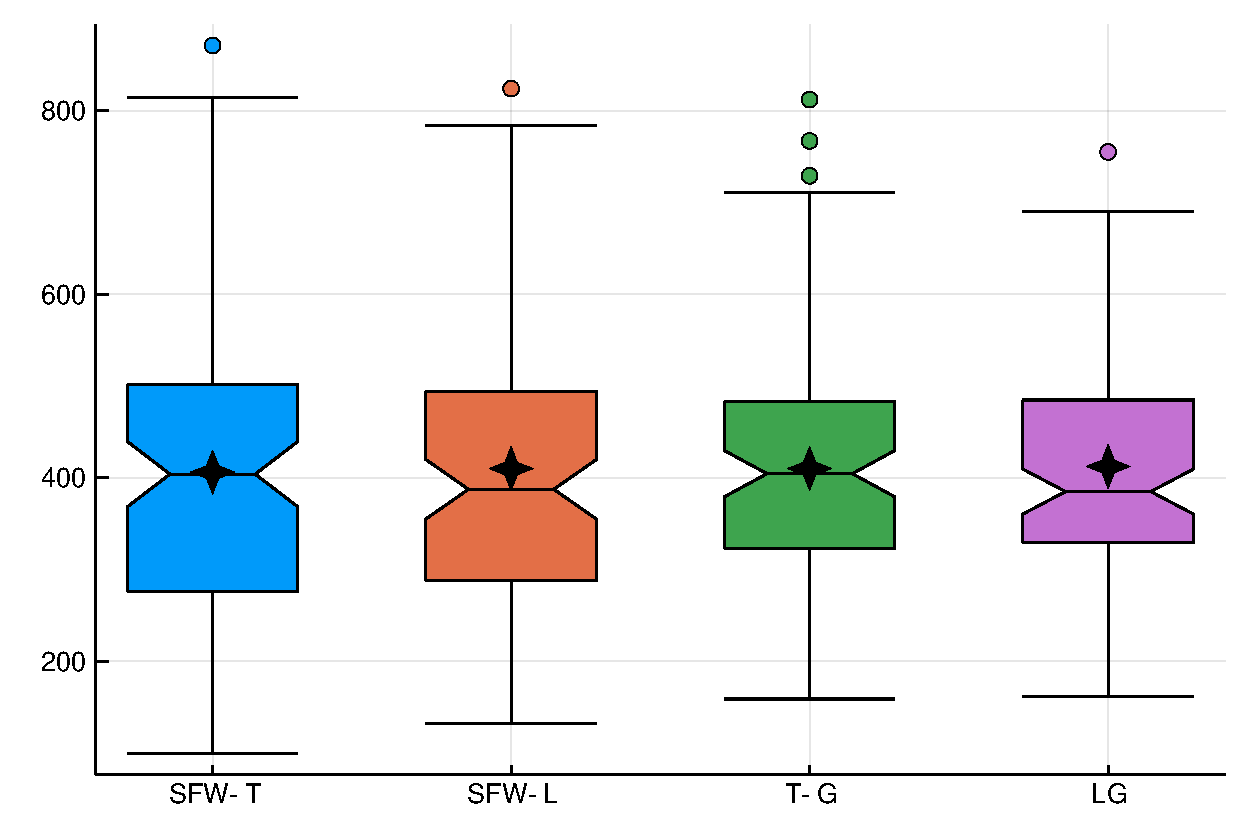
\includegraphics[width=0.33\textwidth]{Chapter4/img/exp_sin_-0000001}
    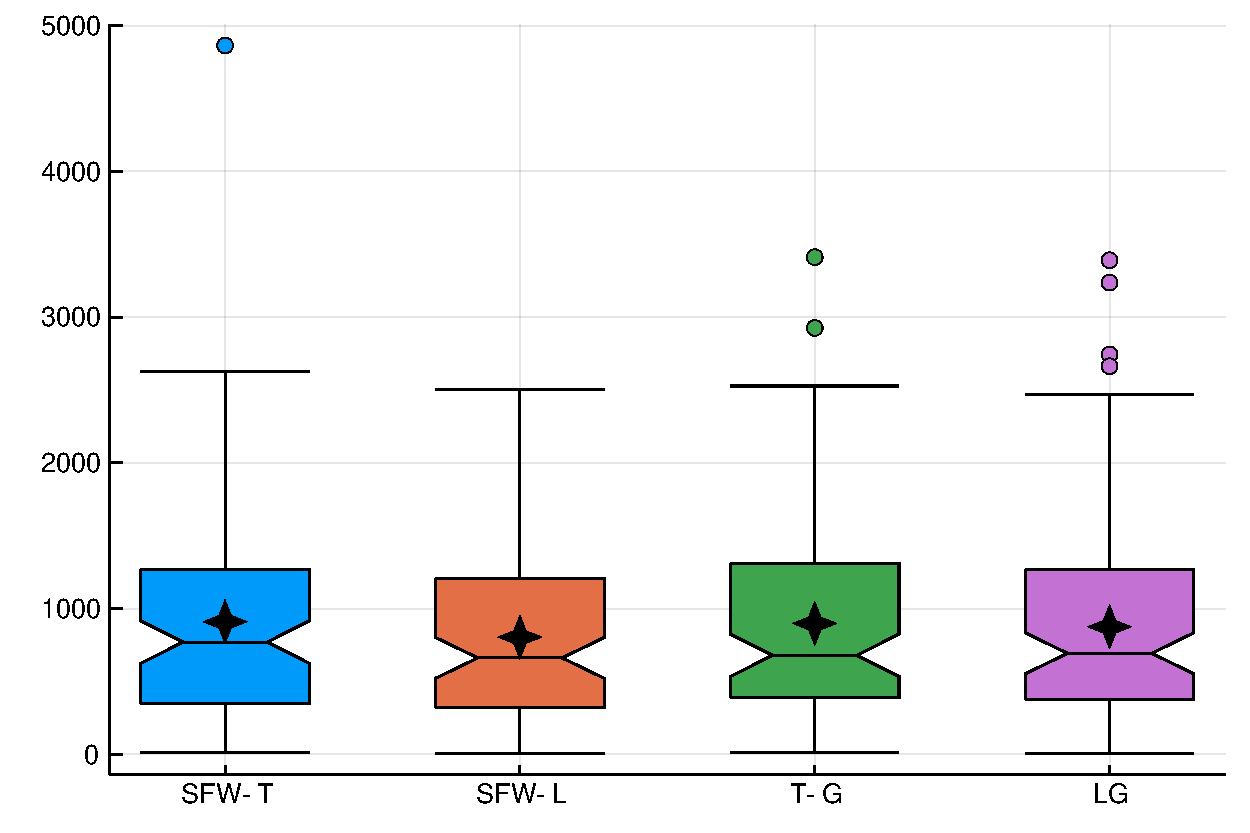
\includegraphics[width=0.33\textwidth]{Chapter4/img/exp_sin_-1}
    \caption{Average stopping time (Left: $d=2,\alpha=\pi/4,\delta=0.0000001$, Right: $d=2,\alpha=0.1,\delta=0.1$), with SFW-T = \SLTCC{}, SFW-L = \SLGapE{}, T-G = \LTCC{}, LG = \LGapE{}.}
    \label{fig:exp1}
\end{figure}


%!TEX root = ../Chapter4.tex
\section{Discussion}\label{sec:lgc.discussion}

In this chapter, we designed the first practically usable asymptotically optimal sampling rules for the pure exploration game for finite-arm linear bandits. Whether the boundedness assumption is necessary to obtain optimal algorithms remains an open question.

Note that since the publication of our work, several other asymptotically optimal algorithms have been proposed~\citep{zaki2020linear,jedra2020linear,katz-samuels2020practical}. Particularly, \cite{jedra2020linear} and \cite{katz-samuels2020practical} also study the fixed-budget setting for linear bandits BAI. Later, \cite{yang2021linear} propose a minimax optimal algorithm for fixed-budget BAI.

More generally, however, the part of fixed-confidence pure exploration algorithms that needs an improvement the most is the stopping rule. While the one we used guarantees $\delta$-correctness, it is very conservative. Indeed, the experimental error rates of algorithms using that stopping rule are orders of magnitude below $\delta$. This means that the concentration inequality does not reflect the query we seek to answer. It quantifies deviations of the $d$-dimensional estimate in all directions (morally, along $2^d$ directions). However, for the usual BAI setting with $d$ arms in an orthogonal basis, it would be sufficient to control the deviation of that estimator in $d-1$ directions to make sure that $i^*(\theta) = i^*(\hat{\theta}_t)$.

Finally, the good performance of \LGapE raises the natural question of whether it could be proven to have similar asymptotic optimality.

% \section{Discussion}\label{sec:conclusion}
%
% %\begin{itemize}
% %\item Fast rates for saddle point computation?
% %\item Changing arm sets? well defined? not clear.
% %\item exploration can be used as subroutine in a regret minimization algorithm
% %\end{itemize}
%
% \paragraph{Computational complexity} First note that the complexity of one step of \LG is $O( C(\text{stopping rule} +A))$ In BAI, the complexity of one step of \LGC (or \LG) is dominated by computing the best response for nature. Indeed, even in the unbounded case, it involves the inversion of a new matrix $V_{w_s^i}$
%
%
%
% \paragraph{Stopping rule} More generally, the aspect of fixed confidence pure exploration that needs an improvement the most is the stopping rule. While the one used here guarantees $\delta$-correctness, it is very conservative. Indeed, the experimental error rates of algorithms using that stopping rule are orders of magnitude below $\delta$. There are at least two ways to devise better stopping rules. First, the threshold $\beta(t,\delta)$ such that for all $t$, $\Vert \theta - \hat{\theta} \Vert^2_{V_{N_t}} \le \beta(t,\delta)$, could perhaps be made smaller. Second and most importantly, that concentration inequality does not reflect the query we seek to answer. It quantifies deviations of the $d$-dimensional estimate in all directions (morally, along $2^d$ directions). However, for the usual best-arm identification setting with $d$ arms in an orthogonal basis, it would be sufficient to control the deviation of that estimator in $d-1$ directions to be sure that $i^*(\theta) = i^*(\hat{\theta}_t)$.


% \newpage
% \bibliographystyle{plainnat}
% \bibliography{Major,manual_bib}
% \newpage

	%%%%%%%%%%%%%%%%%%%%%%%%%%%%%%%%%%%%%%%%%%%%%%%%%%%%%%%%%%%%%%%%%%%%%%%%%%%%%%%%%%%%%%%%%%%%%%
%%									Chapitre 5												%
%%%%%%%%%%%%%%%%%%%%%%%%%%%%%%%%%%%%%%%%%%%%%%%%%%%%%%%%%%%%%%%%%%%%%%%%%%%%%%%%%%%%%%%%%%%%%

\chapter{Hierarchical Bandits for Black-Box Optimization}\label{chap:gpo}
	\citationChap{
		blabla
	}{}
	\minitoc
	\newpage

%%%%%%%%%%%%%%%%%%%%%%%%%%%%%%%%%%%%%%%%%%%%%%%%%%%%%%%%%%%%%%%%%%%%%%%%%%%%%%%%%%%%%%%%%%%%%



% Début du chapitre
\addtocontents{toc}{\protect\setcounter{tocdepth}{1}}
% !TEX root = ../Chapter5.tex
\section{Introduction}\label{sec:gpo.intro}

In this chapter, we deviate our focus a bit. We are still interested in identifying the best arm, but this time among an infinite number of candidates. The search space can be countably infinite or even continuous. That is the global optimization. 

\gls{go} has applications in several domains including hyper-parameter tuning \citep{jamieson2016hyperband, li2017hyperband,samothrakis2013} which is the main topic of Chapter~\ref{CHAP:DTTTS}. \gls{go} usually consists of a data-driven optimization process over an expensive-to-evaluate function. It is also known as \gls{bbo} since the inner behavior of a function is often unknown.

Contrary to Chapter~\ref{CHAP:T3C} and Chapter~\ref{CHAP:LGC}, we are interested in a budgeted setting in this Chapter as we are subject to a high resource-consuming target, hence a pre-defined budget limit can be favored. In budgeted function optimization, a learner optimizes a function $f: \cX \rightarrow \R$ depending on a number of function evaluations limited by $N$ which are sequentially selected. For each of the $N$ evaluations, at round $n$, the learner
picks an element $x_n\in\cX$ and observes a real number $r_n$, where 
\[
    r_n = f(x_n) + \epsilon_n\,,
\]
with $\epsilon_n$ is the noise (see also Definition~\ref{def:mab.go}). The true function value $f(x)$ can thus be interpreted as the arm mean of $x$ using MAB terminology. 

Based on $\epsilon_n$, we can distinguish \emph{deterministic} feedback setting and \emph{stochastic} feed setting. For deterministic feedback, the function evaluations are noiseless (see e.g.~\citealt{defreitas2012gp} for motivation and applications). We pay our attention to the stochastic setting where the noise is assumed to be independent from past observations: $\EE{r_n|x_n} = f(x_n)$.

Treating the problem without any further assumption would be a \emph{mission impossible}. However, the setting gets easier if we assume a global smoothness of the reward function~\citep{agrawal1995continuum,kleinberg2004nearly,kleinberg2008multi,cope2009,auer2007improved,slivkins2011taxonomy,kleinberg2013}. A weaker condition is some \emph{local} smoothness where only neighborhoods around the maximum are required to be smooth.  In fact, local smoothness is sufficient for achieving near-optimality~\citep{valko2013stosoo,azar2014online,grill2015poo,bull2015adaptive}.
We base our work on optimistic tree-based optimization algorithms \citep{munos2011soo,valko2013stosoo,preux2014bandits,azar2014online} that approach the problem with a hierarchical partitioning of the arm space and take the \textit{optimistic principle}. This idea comes from \textit{planning} in Markov decision processes~\citep{kocsis2006bandit,munos2014,grill2016trail}.

Our work is motivated by the \textbf{p}arallel \textbf{o}ptimistic \textbf{o}ptimization (\POO) approach proposed by \citet{grill2015poo},  that \emph{adapts to the smoothness} without the knowledge of it. \POO is a \textit{meta-algorithm} which can be used on top of any hierarchical optimization algorithm that \emph{knows the smoothness}, that we call a subroutine. Not only does \POO require only the mildest local regularity conditions, but it also gets rid of the unnecessary metric assumption that is often required. Local smoothness naturally covers a larger class of functions than global smoothness, yet still assures that the function does not decrease too fast around the maximum. We highlight that the analysis of \POO is modular: Assuming the subroutine has a regret of order $R_n$ \emph{under a local smoothness assumption with respect to a fixed partitioning} (\citealt{grill2015poo}, Assumption~\ref{ass1}, formally introduced in Section~\ref{sec:gpo.pre}), \POO run with such subroutine has a regret bounded by $R_n \sqrt{\log n}$. \POO was originally analyzed using \HOO as a subroutine. However, unlike what \citet{grill2015poo} hypothesize, it is non-trivial to provide a regret bound for \HOO under Assumption~\ref{ass1}. We elaborate on that in Section~\ref{sec:gpo.hct}. In order to validate \POO,  there needs to exist a subroutine with a  regret guarantee that is provable under Assumption~\ref{ass1}. This is what we deliver.

In particular, we prove that \HCT-$\operatorname{iid}$\footnote{Denoted by \HCT in the rest of the paper since we do not consider the correlated feedback setting.} of~\cite{azar2014online} satisfies the required regret guarantee, and is, therefore, a desirable subroutine to be plugged in \POO. Similar to \HOO, \HCT is a hierarchical optimization algorithm based on confidence intervals. However, unlike \HOO, these confidence intervals are obtained by repeatedly sampling a representative point of each cell in the partitioning before splitting the cell. This yields partition trees that have a \emph{controlled depth}, which are easier to analyze under a local smoothness assumption with respect to the partitioning. Whether \HOO has similar regret guarantees under the desired local metricless assumption remains an open question.

\POO requires the subroutine to have a \emph{cumulative} regret guarantee. In this paper, we also provide a more general wrapper for algorithms that only have guarantee for their simple regret, called \GPO (for \textbf{g}eneral \textbf{p}arallel \textbf{o}ptimization). We show that with a cross-validation scheme instead of the original recommendation strategy, any hierarchical bandit algorithm with simple regret guarantee can be plugged into \GPO with only a tiny increase in the resulting simple regret.

%\paragraph{Outline.}
%We first formulate the sequential optimization problem and introduce some preliminary notions and assumptions in Section~\ref{sec:gpo.pre}. Our main result is presented in Section~\ref{sec:gpo.hct}, where we provide a regret upper bound for \HCT under local smoothness with respect to the partitioning. In Section~\ref{sec:gpo.pct}, we present the instantiation of \POO studied in the paper that we call \PCT, in which the underlying subroutine \HOO is replaced by \HCT. We show that \PCT enjoys the same regret bound as \HCT up to a $\sqrt{\log n}$ factor. The general wrapper and its simple regret analysis are presented in Section~\ref{sec:gpo.gpo}. We conclude by some numerical simulations in Section~\ref{sec:gpo.experiments}.

%\todomi{I  suggest carefully and consistently applying editorial comments of Michael Littman: \url{http://cs.brown.edu/~mlittman/etc/style.html}.For example, you are using  citations as nouns.}


% !TEX root = ../Chapter5.tex
\section{Required Assumptions}\label{sec:gpo.pre}

\subsection{General assumptions}\label{sec:gpo.pre.general}
%We introduce notions and assumptions related to our instantiation of \POO.
%\subsection{Problem formulation of black-box optimization}
Let $\cX$ be a measurable space. Our goal is to find the maximum of an unknown noisy function $f:\cX\rightarrow\R$ of which the cost of evaluation is high, given a total budget of $N$ evaluations. At each round $n$, a learner selects a point $x_n\in\cX$ and observes a reward $r_n\triangleq f(x_n)+\epsilon_n$. We make the following assumption on the noise in this thesis. More discussions on the role and impact of noise are provided by~\cite{bartlett2019simple}.
\begin{assumption}
\begin{leftbar}[assumptionbar][bounded, independent and conditionally centered noise]
We assume that the noise $\epsilon_n$ is bounded by $[0,1]$, independent from previous observations and such that 
\[
    \EE{\epsilon_n|x_n} = 0\,.
\]
\end{leftbar}
\end{assumption}

%\footnote{our analysis can be easily extended to cover centered sub-Gaussian noise}.
After $N$ evaluations, the algorithm outputs a guess for the maximizer, denoted by $x(N)$. $x(N)$ is indeed the decision rule $J_N$ in the learning protocol of a general pure-exploration problem. We assume that there exists at least one $x^\star \in \cX$ s.t.\,$f(x^\star) \triangleq \sup_{x\in\cX} f(x)$, denoted by $f^\star$ in the following. We measure the performance by the simple regret. We can particularize Definition~\ref{def:mab.simple_regret} of simple regret into the setting of this chapter:
\[
	S_N \triangleq f^\star - f(x(N))\,.
\]
Likewise, we can also particularize the notion of cumulative regret into our setting:
\[
	R_N \triangleq Nf^\star - \sum_{n=1}^N f(x_n)\,.
\]

\subsection{Covering tree that guides the optimization}\label{sec:gpo.pre.tree}

Hierarchical bandits rely on the existence of hierarchical partitioning $\mathcal{P}\triangleq\{\mathcal{P}_{h,i}\}_{h,i}$ defined recursively, where
\[
	\mathcal{P}_{0,1} = \mathcal{X},  \ \ \ \
	\mathcal{P}_{h,i} = \bigcup_{j=0}^{K-1} \mathcal{P}_{h+1,Ki-j}.
\]
Such a partition can be naturally represented by a tree, where $K$ denotes the maximum number of children of a node in that tree. Many of known algorithms depend on a metric/dissimilarity over the search space to define the regularity assumptions that link the partitioning to some \gls{near-optimality dimension}, that is independent of the partitioning. However, this was shown to be artificial~\citep{grill2015poo}, since (i) the metric is not fully exploited by the algorithms and (ii) the notion of near-optimality dimension independent of partitioning is ill-defined.
Hence, it is natural to make smoothness assumptions directly related only to the partitioning.

We now present \emph{the only regularity assumption} on the target function $f$ that is expressed in terms of the partitioning $\cP$ given in Assumption~\ref{ass:gpo.local}.

\begin{assumption}
\begin{leftbar}[assumptionbar][local smoothness w.r.t.\,$\cP$]\label{ass:gpo.local}
For $x^\star$ be a global maximizer, we denote by $i_h^\star$ be the index of the only cell at depth~$h$ that contains $x^\star$.
Then, there exist a global maximizer $x^\star$ and two constants $\nu > 0,$ $\rho\in (0,1)$ s.t.,
\[
	\forall h\geq 0, \forall x\in\mathcal{P}_{h,i_h^\star}, \ \  f(x)\geq f^\star - \nu\rho^h.
\]
\end{leftbar}
\end{assumption}
Note that this assumption is the same as the one of~\cite{grill2015poo}. Multiple maximizers may exist, but this assumption needs to be satisfied only by one of them.

We stress again that requiring only a \textbf{local} smoothness assumption is an improvement since (i) it is a one-side local Lipschitz-type of assumption that naturally covers a larger class of functions, (ii) it only constrains $f$ along the optimal path of the covering tree which is a plausible property in an optimization scenario, and (iii) shows that the optimization is actually easier than it was previously believed. 

Besides, in this chapter, we aim to design algorithms that does not rely on any metric. Previous methods all depend on a metric, and their smoothness assumptions are summarized in Table~\ref{table:hoo}.

\begin{table*}[ht]
\centering
%\def\arraystretch{1.5}
\begin{tabular}[r]{|r|cc|} 
\hline
& \textbf{global} smoothness & \textbf{local} smoothness \\ \hline
\specialcell{\textbf{known} smoothness} &\Zooming, \HOO & \DOO, \HCT \\
\hline
\specialcell{\textbf{unknown} smoothness} &\TZ &
\SOO, \StoSOO, \ATB \\
\hline
\end{tabular}
\caption{Smoothness assumptions for hierarchical bandits algorithms.}
\label{table:hoo}
\end{table*}

As first observed by~\cite{auer2007improved}, the difficulty of a \gls{go} should depend on the size of near-optimal regions and on how fast they shrink. \citet{auer2007improved} use a margin condition that quantifies this difficulty by the volume of near-optimal regions. In this work, we use a similar notion of \gls{near-optimality dimension}\footnote{The present definition is slightly different from the original \POO paper, where a coefficient 3 is present instead of 2 due to a technical detail.} instead. This notion is directly related to the partitioning.
%\begin{definition}[near-optimality dimension w.r.t.\,$\cP$]\label{defNearOpt} We define the near-optimality dimension of~f with respect to \,$\cP$ as
%\[
%	d(\nu,\rho) \triangleq \inf\{d'\in\mathbb{R}^+ : \exists C > 0,\forall h \geq 0, \mathcal{N}_h(3\nu\rho^h) \leq C\rho^{-d'h}\},\footnote{This definition is slightly different from the original \POO paper, where a coefficient 3 is present instead of 2 due to a technical detail.}
%\]
%where $\mathcal{N}_h(\epsilon)$ is the number of cells $\mathcal{P}_{h,i}$ s.t.\,$\sup_{x\in\mathcal{P}_{h,i}}f(x) \geq f^\star - \epsilon$.
%\end{definition}
%$\mathcal{N}_h(3\nu\rho^h)$ can be thought as the number of cells that any algorithm needs to sample in order to find the maximum. A smaller $d(\nu,\rho)$ implies an easier optimization problem. In addition, we define a set $\cC$ depending on $\nu$ and $\rho$,
%\[
%	\cC(\nu,\rho) \eqdef \left\{C>0: \forall h \geq 0, \mathcal{N}_h(3\nu\rho^h) \leq C\rho^{-d(\nu,\rho)h} \right\}\!,
%\]
%and we let $C(\nu,\rho) \eqdef \inf\cC(\nu,\rho)$.

\begin{definition}
\begin{leftbar}[defnbar][near-optimality dimension w.r.t.\,$\cP$]\label{defNearOpt} 
For any $\nu > 0$, $C>1$, and $\rho \in (0,1)$, we define the near-optimality dimension of~f with respect to \,$\cP$ as
\[
	d(\nu,C, \rho) \triangleq \inf\left\{d'\in\mathbb{R}^+ : \forall h \geq 0, \mathcal{N}_h(3\nu\rho^h) \leq C\rho^{-d'h}\right\}\,,
\]
where $\mathcal{N}_h(\epsilon)$ is the number of cells $\mathcal{P}_{h,i}$ such that $\sup_{x\in\mathcal{P}_{h,i}}f(x) \geq f^\star - \epsilon$.
\end{leftbar}
\end{definition}
$\mathcal{N}_h(3\nu\rho^h)$ can be thought as the number of cells that any algorithm needs to sample in order to find the maximum. A smaller $d(\nu,C,\rho)$ implies an easier optimization problem.
% In addition, we define a set $\cC$ depending on $\nu$ and $\rho$,
%\[
%	\cC(\nu,\rho) \eqdef \left\{C>0: \forall h \geq 0, \mathcal{N}_h(3\nu\rho^h) \leq C\rho^{-d(\nu,\rho)h} \right\}\!,
%\]
%and we let $C(\nu,\rho) \eqdef \inf\cC(\nu,\rho)$.



% !TEX root = ../Chapter5.tex
\section{\HCT{} under Local Smoothness w.r.t. \texorpdfstring{$\cP$}{}}\label{sec:gpo.hct}

Analyzing \HOO under Assumption~\ref{ass1} is not trivial. A key lemma in the analysis of \HOO  (Lemma~3 by \citealt{bubeck2011pure}) that controls the variance of near-optimal cells \emph{is not true} under local smoothness assumptions as Assumption~\ref{ass1}. Indeed, \HOO could induce a very deep covering tree,  while producing too many nodes that are neither near-optimal nor sub-optimal. The concept of near-optimal and sub-optimal nodes is then characterized by the \emph{sub-optimality gap} of each node which measures the distance between the local maximum of the node and the global maximum. Intuitively, nodes that are neither near-optimal nor sub-optimal represent the nodes of whom the sub-optimality gap is neither too large nor too small. To control the regret due to these nodes,~\cite{bubeck2011pure} use global smoothness (weakly Lipschitz) assumption. Assumption~\ref{ass1} is weaker, only local, and does not offer such comfort. If we want to control the regret due to these nodes without Lemma~3 of \citet{bubeck2011pure}, one possible way is to control the depth of the covering tree to ensure that we do not have too many of them. In particular, another algorithm known as \HCT \citep{azar2014online} implies a controlled depth of the tree which allows it to be analyzed under Assumption~\ref{ass1} as opposed to \HOO. We now give a brief description of \HCT and present a new analysis of it.

\subsection{Description of \HCT{}}
\begin{algorithm}[ht]
\centering
\caption{Algorithm of \HCT{}}
\label{alg:hct}
\begin{algorithmic}[1]
    \State {\bfseries Input:} $K$, $\nu>0$, $\rho\in(0,1)$, $c>0$, tree partitioning $\{\mathcal{P}_{h,i}\}$, confidence $\delta$
    \State {\bfseries Initialization:} $\mathcal{T}_1 \gets \{(0,1),(1,1),\ldots,(1,K)\}$, $U_{1,1}(1) \gets \cdots \gets U_{1,K}(1) \gets +\infty$
    \For{$t \gets 1 \ldots n$}
        \If{$t=t^+$}
            \For{$(h,i)\in\mathcal{T}_t$}
                \State $U_{h,i}(t) \gets \hat{\mu}_{h,i}(t) + \nu\rho^{h} + c\sqrt{\frac{\operatorname{log}\left(1/\tilde{\delta}(t^+)\right)}{T_{h,i}(t)}}$
            \EndFor
            \State \texttt{UpdateBackward}$(\cT_t, t)$
        \EndIf
        \State $(h_t,i_t),P_t \gets$ \texttt{OptTraverse}($\cT_t, t$)
        \State \text{Evaluate} $x_{h_t,i_t}$ and obtain $r_t$
        \State $T_{h_t,i_t}(t) \gets T_{h_t,i_t}(t)+1$
        \State \text{Update} $\hat{\mu}_{h_t,i_t}(t)$
        \State $U_{h_t,i_t}(t) \gets \hat{\mu}_{h_t,i_t}(t) + \nu\rho^{h_t} + c\sqrt{\frac{\operatorname{log}\left(1/\tilde{\delta}(t^+)\right)}{T_{h_t,i_t}(t)}}$
        \State \texttt{UpdateBackward}($P_t, t$)
        \State $\tau_{h_t}(t) \gets \ceil{\frac{c^2\operatorname{log}(1/\tilde{\delta}(t^+))}{\nu^2}\rho^{-2h_t}}$
        \If{$T_{h_t,i_t}(t)\geq\tau_{h_t}(t)$ and $(h_t,i_t)$ is a leaf}
            \State \text{Expand} the node $(h_t,i_t)$
        \EndIf
    \EndFor
\end{algorithmic}
\end{algorithm}

\begin{algorithm}[ht]
\centering
\caption{Subroutine \texttt{OptTraverse} of \HCT{}}
\label{alg:hct_opt}
\begin{algorithmic}[1]
    \State {\bfseries Input:} a tree $\cT$, round $t$
    \State {\bfseries Initialization:} $(h,i)\leftarrow (0,1)$; $P\leftarrow \{(0,1)\}$; $T_{0,1}(t)=\tau_0(t)=1$
    \While{$(h,i)$ is not a leaf of $\cT$ and $T_{h,i}(t)\geq\tau_h(t)$}
        \State $j \gets \underset{j\in\{0,\ldots,K-1\}}{\argmax} \left\{B_{h+1,Ki-j}(t)\right\}$
        \State $(h,i) \gets (h+1,Ki-j)$
        \State $P\leftarrow P\cup\{(h,i)\}$
    \EndWhile
    \State {\bfseries Return} $(h,i)$ and $P$
\end{algorithmic}
\end{algorithm}

\begin{algorithm}[ht]
\centering
\caption{Subroutine \texttt{UpdateBackward} of \HCT{}}
\label{alg:hct_update}
\begin{algorithmic}[1]
    \State {\bfseries Input:} a tree $\cT$, round $t$ \\ \hfil \emph{note that $P_t$ can also be considered as a tree, thus input of this function}
    \For{$(h,i)\in\cT$ backward from each leaf of $\cT$}
        \If{$(h,i)$ is a leaf of $\cT$}
            \State $B_{h,i}(t) \gets U_{h,i}(t)$
        \Else 
            \State $B_{h,i}(t) \gets \min\left\{U_{h,i}(t),\underset{j\in\{0,\ldots,K-1\}}{\max} \left\{B_{h+1,Ki-j}(t)\right\} \right\}$
        \EndIf
    \EndFor
\end{algorithmic}
\end{algorithm}

The pseudocode of \HCT (Algorithm~\ref{alg:hct}) and two detailed snippets (Algorithm~\ref{alg:hct_opt} and Algorithm~\ref{alg:hct_update}) describe the process of traversing the covering tree.
The algorithm stores a finite subtree $\cT_t$ at each round~$t$ which is initialized by $\cT_0 = \{(0,1)\}$. Each cell is associated with a representative point $x_{h,i}$ and the algorithm keeps track of some statistics regarding this point. One of these statistics is the empirical mean reward $\hat{\mu}_{h,i}(t)$ which is the average on the first $T_{h,i}(t)$ rewards received when querying $x_{h,i}$.
%\[
%	\hat{\mu}_{h,i}(t) \triangleq \frac{1}{T_{h,i}(t)}\sum_{s=1}^{T_{h,i}(t)}r_{(h,i),s},
%\]
The \HCT algorithm also keeps track of an upper confidence bound $U$-value for the cell $(h,i)$,
\[
	U_{h,i}(t) \triangleq \hat{\mu}_{h,i}(t) + \nu\rho^{h} + c\sqrt{\frac{\operatorname{log}(1/\tilde{\delta}(t^+))}{T_{h,i}(t)}}\CommaBin
\]
where $t^+\triangleq2^{\lceil \operatorname{log}_2(t) \rceil}$, $\tilde{\delta}(t)\triangleq\min\{c_1\delta/t,1/2\}$, and its corresponding $B$-value,
\begin{equation*}
	B_{h,i}(t) \triangleq
	\left\{ \begin{array}{ll}
				\min\left\{U_{h,i}(t),\underset{j\in\{0,\ldots,K-1\}}{\max} \left\{B_{h+1,Ki-j}(t)\right\} \right\} & \operatorname{if}~(h,i) \text{ is an internal node,}\\
				U_{h,i}(t) & \operatorname{otherwise,}
			\end{array}\right.
\end{equation*}
which is designed to be a tighter upper confidence bound than the $U$-value. Here, $c$ and $c_1$ are two constants, and $\nu\rho^h$ represents the \emph{resolution}\footnote{The term \emph{resolution} refers to the maximum variation in the cell. If it is too large, then we need to shrink the volume, thus increase the resolution.} of the region $\cP_{h,i}$. Observe that $U_{h,i}(t)$ and $B_{h,i}(t)$ are not updated at every round, but are constant on time intervals of the form $[2^k,2^{k+1})$.

At each round $t$, the algorithm traverses the current covering tree along an \emph{optimistic path}~$P_t$ before choosing a point (\texttt{OptTraverse} function). This optimistic path~$P_t$ is obtained by repeatedly selecting cells that have a larger $B$-value until a leaf or a node that is sampled less than a certain number of times is reached. If a leaf is reached, then this leaf is sampled and expanded (i.e., we split the leaf into $K$ equal-sized regions and initialize their $U$-values to $+\infty$); otherwise, the node that is not sampled enough is re-sampled. All the $B$-values along the optimistic path are then updated backwardly from the current node to the root (\texttt{UpdateBackward} function). More precisely, \HCT{} samples one node a certain number of times $\tau_h(t)$ in order to sufficiently reduce the uncertainty before expanding it. Hence, $\tau_h(t)$ is defined such that the uncertainty over the rewards in $\mathcal{P}_{h,i}$ is roughly equal to the resolution of the node,
\[
	\tau_h(t) \triangleq \ceil{\frac{c^2\operatorname{log}(1/\tilde{\delta}(t^+))}{\nu^2}\rho^{-2h}}.
\]

\subsection{Analysis of \HCT \textbf{under a local \emph{metricless} assumption}}\label{sec:gpo.analysis}
We now state our main theorem. We prove that \HCT achieves an expected regret bound under Assumption~\ref{ass1} which matches the regret bound given by~\cite{azar2014online} up to constants. Moreover, compared to that result, the near-optimality dimension $d$ featured in Theorem~\ref{thm:hct} is the one of Definition~\ref{defNearOpt} that is defined with respect to the partitioning and not with respect to a metric. For a fixed budget $n$, we introduce the notation $\HCT{}(\nu,\rho)$ to refer to the instantiation of $\HCT{}$ parameterized by $\nu$, $\rho$, $c=2\sqrt{1/(1-\rho)}$ and $\delta = 1/n$.

\begin{restatable}{theorem}{restathm}\label{thm:hct}
	Assume that function~$f$ satisfies Assumption~\ref{ass1}. Then, setting $\delta \eqdef 1/n$, the cumulative regret of ${\HCT}(\nu,\rho)$ after $n$ function evaluations is upper bounded as 
\[
	\mathbb{E}[R_n^{\HCT{}(\nu,\rho)}] \leq \alpha C (\operatorname{log}n)^{1/(d(\nu,C,\rho)+2)}n^{(d(\nu,C,\rho)+1)/(d(\nu,C,\rho)+2)}\!,
\]
where $\alpha$ is a numerical constant and $C$ is the constant associated to $d(\nu,C,\rho)$.
%\in\cC(\nu,\rho)$.
\end{restatable}\noindent
As a consequence, by simply applying  the recommendation strategy that follows the distribution of previous plays, we get the following simple-regret bound.
\begin{corollary}\label{col}
The simple regret  of {\HCT} after $n$ function evaluations under Assumption~\ref{ass1} satisfies
\[
	\mathbb{E}[S_n^{\HCT{}(\nu,\rho)}] \leq \alpha C(\operatorname{log}n)^{1/(d(\nu,C,\rho)+2)}n^{-1/(d(\nu,C,\rho)+2)}.
\]
\end{corollary}
We now sketch the proof. The full proof follows the analysis of~\cite{azar2014online} and is detailed in Appendix~\ref{app:gpo.hct}.
As  mentioned above, \HCT has a controlled depth. Indeed, given the threshold $\tau_h(t)$ required at depth $h$, in Section~\ref{proof:lemma_depth}, we prove that the depth of the covering tree is bounded as stated in the following lemma.
\begin{restatable}{lemma}{restalemmadepth}\label{lemma_depth}
The depth of the covering tree produced by \HCT after $n$ function evaluations satisfies \[H(n) \leq H_{\max}(n) \triangleq \ceil{\frac{1}{2(1-\rho)} \operatorname{log}\left( \frac{n\nu^2}{c^2\rho^2} \right)}\!\cdot\]
\end{restatable}
\noindent
Defining the mean reward $\mu_{h,i} \triangleq f(x_{h,i})$, we introduce a favorable event under which the mean reward of all expanded nodes is within a confidence interval,
\[
	\xi_t \triangleq \left\{ \forall (h,i)\in\mathcal{L}_t,  |\hat{\mu}_{h,i}(t) - \mu_{h,i}| \leq c\sqrt{\operatorname{log}(1/\tilde{\delta}(t))/T_{h,i}(t)} \right\}\CommaBin
\]
where $\cL_t$ is the set of all possible nodes in trees of maximum depth $H_{\max}(t)$.

We split the regret into two parts depending on whether $\xi_t$ holds or not.
In Appendix~\ref{proof:lemma_failing}, we prove that the failing confidence term is with high probability bounded by $\sqrt{n}$. In the case when  $\xi_t$ holds, we bound the regret in Appendix~\ref{proof:thm}
by treating separately the two parts, $\Delta_{h_t,i_t}$ and $\hat{\Delta}_t$, of the instantaneous regret $\Delta_t$,
\[
\Delta_t \eqdef f^\star - r_t = f^\star - f(x_{h_t,i_t}) + f(x_{h_t,i_t}) - r_t = \Delta_{h_t,i_t} + \hat{\Delta}_t.
\]
Next, we bound $ \hat{\Delta}_t$ by Azuma-Hoeffding concentration inequality \citep{azuma1967}.
Then, we bound $ \Delta_{h_t,i_t}$  with the help of the following lemma, which is the major difference compared to the original \HCT analysis by~\cite{azar2014online}. In particular, the lemma states that
if Assumption~\ref{ass1} is verified then
 $f^\star$ is upper-bounded by the $U$-value of any optimal node.
\begin{lemma}\label{upper}
	Under Assumption~\ref{ass1} and under event $\xi_t$, we have that for any optimal node $(h^\star,i^\star)$, $U_{h^\star,i^\star}(t)$ is an upper bound on $f^\star$.
\end{lemma}

\begin{proof}
Since $t^+ \geq t$, we have
\[
	U_{h^\star,i^\star}(t) \eqdef \hat{\mu}_{h^\star,i^\star}(t) + \nu\rho^{h^\star} + c\sqrt{\frac{\operatorname{log}(1/\tilde{\delta}(t^+))}{T_{h^\star,i^\star}(t)}} \geq \hat{\mu}_{h^\star,i^\star}(t) + \nu\rho^{h^\star} + c\sqrt{\frac{\operatorname{log}(1/\tilde{\delta}(t))}{T_{h^\star,i^\star}(t)}}\cdot
\]
Moreover, as we are under event $\xi_t$, we also have
\[
	\hat{\mu}_{h^\star,i^\star}(t) + c\sqrt{\frac{\operatorname{log}(1/\tilde{\delta}(t))}{T_{h^\star,i^\star}(t)}} \geq f\left(x_{h^\star,i^\star}\right).
\]
Therefore, $U_{h^\star,i^\star}(t) \geq f(x_{h^\star,i^\star}) + \nu\rho^{h^\star} \geq f^\star$.
\end{proof}
\noindent With the help of Lemma~\ref{upper} (see Step 2 in Appendix~\ref{proof:thm}), we can then upper bound $\Delta_{h_t,i_t}$ as
\[
\Delta_{h_t,i_t} \leq 3c\sqrt{\frac{\operatorname{log}(2/\tilde{\delta}(t))}{T_{h_t,i_t}(t)}}\cdot%\CommaBin
\]
To bound the total regret of the all nodes selected, we divide them
into two categories, depending on whether their depth is smaller or equal than $\bar H$
(to be optimized later) or not.

For the nodes in depths $h \leq \bar H$, we  use
Lemma~\ref{upper} again, now to show that \texttt{OptTraverse} only selects nodes
 %\begin{equation*} %\label{eq14}
%\Delta_{h_t^p,i_t^p} \leq 3\nu\rho^{h_t^p},
%\end{equation*}
that have a parent which is $(3\nu\rho^{h_t-1})$-optimal.
For the nodes for which  $h > \bar H$, we bound the regret using the
selection rule of \HCT.


The sums of the regrets from the two categories are proportional
and inversely proportional to an increasing function of $\bar H$.
By finding the value of $\bar H$ for which the sum of the two
terms reaches its minimum and adding the regret coming
from the situations where the favorable event does not hold,
gives us the following cumulative regret for \HCT: With probability $1-\delta$,
\[
	R_n^{\HCT(\nu,\rho)} \leq \cO\left( (\operatorname{log}(n/\delta))^{1/(d(\nu,C,\rho)+2)}n^{(d(\nu,C,\rho)+1)/(d(\nu,C,\rho)+2)} \right).
\]
However, the analysis of \POO requires a bound on the expected regret of the underlying subroutine. For that purpose, we simply set $\delta \eqdef 1/n$ and that gives us the statement of Theorem~\ref{thm:hct}, and consequently Corollary~\ref{col}.


% !TEX root = ../Chapter5.tex
\section{\texorpdfstring{\PCT}{} That Does Not Need to Know the Smoothness}\label{sec:gpo.pct}

In this section, we formally introduce a generic $\POO(\cA)$ algorithm, taking as input \emph{any} algorithm $\cA=\cA(\nu,\rho)$ requiring the smoothness parameters. We provide a simple regret upper bound for a particular instantiation called \PCT, for \POO\!(\HCT).

\subsection{Generic parallel optimistic optimization}

$\POO(\cA)$ (\textbf{p}arallel \textbf{o}ptimistic \textbf{o}ptimization) is a meta-algorithm that uses any hierarchical optimization algorithm $\cA$ that knows the smoothness as a subroutine, originally proposed by \cite{grill2015poo} for $\cA = \HOO$. In this algorithm, several instances of $\cA$ are run in parallel, each one using a different pair of parameters $(\nu,\rho)$ in a well-chosen grid~$\cG$ (defined in Line~4 of Algorithm~\ref{alg:pct}). In the end, $\POO(\cA)$ chooses the instance that has the largest empirical mean reward and returns one of the points evaluated by this instance, chosen uniformly at random.

The pseudo-code of $\POO(\cA)$ is shown in Algorithm~\ref{alg:pct}. Additionally to the base algorithm itself, it requires two parameters $\rho_{\max}$ and $\nu_{\max}$ that determine the range of $\cA(\nu,\rho)$ instances that we can compete with. However, these parameters can be set as a function of the number of evaluations as explained in details in Appendix C of~\cite{grill2015poo}, hence not mandatory in practice. An important remark is that given a budget $n$ of function evaluations, the number of $\cA$ instances $N$ run by $\POO(\cA)$ depends on $n$, and each instance is run for $\floor{n/N(n)}$ times. Due to the doubling scheme used in Lines~2-10, note however that $\POO(\cA)$ does not need to know this total number of function evaluations. Hence, if the base algorithm $\cA$ is anytime, so is $\POO(\cA)$.

\begin{algorithm}[ht]
\centering
\caption{$\POO(\cA)$ - parallel optimistic optimization with base algorithm $\cA$}
\label{alg:pct}
\begin{algorithmic}[1]
    \State {\bfseries Input:} base algorithm $\cA$, $\nu_{\max}$,$\rho_{\max}$, branching factor of the partitioning $K$
    \State {\bfseries Initialization:} $D_{\max} \gets \ln K/\ln\left( 1/\rho_{\max}\right)$, number of function evaluations $n \gets 0$, current number of instances of $\cA$: $N \gets 1$, $\mathcal{S} \gets \{(\nu_{\max},\rho_{\max})\}$
    
    \While{budget still available}
        \While{$N \le \tfrac{1}{2}D_{\max}\log\left(n/(\log n)\right)$}
            \For{$i\gets1, \dots, N$}
        		\State $s \gets \left(\nu_{\max},{\rho_{\max}}^{2N/(2i+1)}\right)$
        		\State \texttt{initialize} $\cA(s)$ (if not already done before) 
        		\State \texttt{continue running} $\cA(s)$ \texttt{until it has given} $\frac{n}{N}$ \texttt{rewards} $r_{s,1},\ldots,r_{s,n/N}$.
        		\State \texttt{compute} $\widehat{\mu}[s] = \frac{N}{n}\sum_{i=1}^{n/N}r_{s,i}.$
        	\EndFor
            \State $n \gets 2n$
            \State $N \gets 2N$
        \EndWhile
        \State \texttt{perform each $\cA(s)$ once} 
        \State \texttt{update} $\widehat{\mu}[s]$
        \State $n \gets n+N$
    \EndWhile
    \State $s^\star \gets \argmax_{s\in\mathcal{S}}~\widehat{\mu}[s]$
    \State {\bfseries Return} A point sampled u.a.r.\,from the points evaluated by $\cA(s^\star)$
\end{algorithmic}
\end{algorithm}

\subsection{Upper bound on the simple regret of \PCT{}}

Building on our new analysis of the \HCT algorithm, we are able to provide theoretical guarantees for the resulting $\POO(\HCT)$ algorithm, that we refer to as \PCT (\textbf{p}arallel \textbf{c}onfidence \textbf{t}ree). More precisely we define $\PCT(\delta)$ as \POO run on top of \HCT using confidence parameter~$\delta$.

Letting $(\nu^\star,C^\star,\rho^\star)$ be a triple of parameters for which Assumption~\ref{ass1} is true, we prove that \PCT achieves a regret that is comparable to the one obtained by $c$.

%\todo[inline]{below a formula for $N(n)$ is needed}

\begin{theorem}\label{thm:pct}
Assume that the target function $f$ satisfies Assumption~\ref{ass1} and $\nu^\star \leq \nu_{\max}$ and $\rho^\star \leq \rho_{\max}$. For $\delta = N(n)/n$ with $N(n) = \lceil (1/2)D_{\max}\log(n/\log n)\rceil$, the simple regret of $\PCT(\delta)$ after $n$ function evaluations is bounded as
\[
	\mathbb{E}[S_n^{\PCT(\delta)}]  \leq \beta D_{\max}(\nu_{\max}/\nu^\star)^{D_{\max}} \left( ((\log^2 n)/n)^{1/(d(\nu^{\star},C^\star,\rho^{\star})+2)} \right),
\]
where $\beta$ is a constant independent of $\nu_{\max}$ and $\rho_{\max}$.\footnote{More generally, Theorem~\ref{thm:pct} holds for any $\nu \leq \nu_{\max}$ and $\rho \leq \rho_{\max}$.}
\end{theorem}
By Corollary~\ref{col}, we know that the simple regret of \HCT after $n$ function evaluations run with $(\nu^\star,C^\star,\rho^\star)$ is of order $\cO\left( (\log n/n)^{1/(d(\nu^{\star},C^\star,\rho^{\star})+2)} \right)$. As a consequence, the performance of \PCT is at most a $\sqrt{\log n}$ factor away from that of the best \HCT instance.

Theorem~\ref{thm:pct} follows from Corollary~\ref{col} and Proposition~\ref{prop:WrapperPOO} below. This wrapper result highlights how cumulative regret guarantees for \emph{any} base algorithm translate into simple regret guarantees for the corresponding $\POO(\cA)$ algorithm. Its proof almost replicates the analysis of \POO{}(\HOO) by \cite{grill2015poo} and we provide it in Appendix~\ref{app:gpo.poo} for the sake of completeness.  

\begin{proposition}\label{prop:WrapperPOO} If for all $(\nu,\rho)$ the $\cA(\nu,\rho)$ algorithm has its \emph{cumulative regret} bounded as
\begin{equation}
    \mathbb{E}\left[R_n^{\cA(\nu,\rho)}\right] \leq \alpha C(\log n)^{1/(d(\nu,C,\rho)+2)}n^{(d(\nu,C,\rho)+1)/(c+2)},\label{centralConditionPOO}
\end{equation}
for any function $f$ satisfying Assumption~\ref{ass1} with parameters $(\nu,C,\rho)$, then there exists a constant $\beta$ that is independent of $\nu_{\max}$ and $\rho_{\max}$ such that 
\[
    \mathbb{E}\left[S_n^{\POO(\cA)}\right]  \leq \beta D_{\max}(\nu_{\max}/\nu^\star)^{D_{\max}} \left( (\log^2 n)/n)^{1/(d(\nu^\star,C^\star,\rho^\star)+2)} \right)\!,
\]
for any function $f$ satisfying Assumption~\ref{ass1} with parameters $\nu^\star \leq \nu_{\max}$ and $\rho^\star\leq \rho_{\max}$.
\end{proposition}


% !TEX root = ../Chapter5.tex
\section{General Parallel Optimization}\label{sec:gpo.gpo}

We present our new wrapper in this section. In order to get a better understanding, we start with a brief introduction of \gls{poo}.

\subsection{Generic parallel optimistic optimization}\label{sec:gpo.gpo.generic}

We introduce $\gls{poo}(\cA)$ as a generic  algorithm, taking as input \emph{any} hierarchical optimization algorithm $\cA=\cA(\nu,\rho)$ requiring the smoothness parameters.

$\gls{poo}(\cA)$ is a meta-algorithm that uses $\cA$ that knows the smoothness as a subroutine, originally proposed by~\cite{grill2015poo} for $\cA = \gls{hoo}$. In this algorithm, several instances of $\cA$ are run in parallel, each one using a different pair of parameters $(\nu,\rho)$ in a well-chosen grid~$\cG$ (defined in Line~4 of Algorithm~\ref{alg:pct}). In the end, $\gls{poo}(\cA)$ chooses the instance that has the largest empirical mean reward and returns one of the points evaluated by this instance, chosen uniformly at random.

The pseudo-code of $\POO(\cA)$ is shown in Algorithm~\ref{alg:pct}. Additionally to the base algorithm itself, it requires two parameters $\rho_{\max}$ and $\nu_{\max}$ that determine the range of instances $\cA(\nu,\rho)$ that we can compete with. However, these parameters can be set as a function of the number of evaluations as explained in details in Appendix C of~\cite{grill2015poo}, hence not mandatory in practice. An important remark is that given a budget $N$ of function evaluations, the number of instances $M$ run by $\gls{poo}(\cA)$ depends on $N$, and each instance is run for $\floor{N/M(N)}$ times. Due to the doubling scheme used in Lines~2-10 of Algorithm~\ref{alg:gpo}, note however that $\gls{poo}(\cA)$ does not need to know this total number of function evaluations. Hence, if the base algorithm $\cA$ is anytime, so is $\gls{poo}(\cA)$.

\begin{algorithm}[ht]
\centering
\caption{Algorithm of $\POO(\cA)$ with base algorithm $\cA$}
\label{alg:pct}
\begin{algorithmic}[1]
    \State {\bfseries Input:} base algorithm $\cA$, $\nu_{\max}$,$\rho_{\max}$, branching factor of the partitioning $K$
    \State {\bfseries Initialization:} $D_{\max} \gets \ln K/\ln\left( 1/\rho_{\max}\right)$, number of function evaluations $n \gets 0$, current number of instances of $\cA$: $N \gets 1$, $\mathcal{S} \gets \{(\nu_{\max},\rho_{\max})\}$
    
    \While{budget still available}
        \While{$N \le \tfrac{1}{2}D_{\max}\log\left(N/(\log N)\right)$}
            \For{$i\gets1, \dots, N$}
        		\State $s \gets \left(\nu_{\max},{\rho_{\max}}^{2M/(2i+1)}\right)$
        		\State \text{Initialize} $\cA(s)$ (if not already done before) 
        		\State \text{Continue running} $\cA(s)$ \text{until it has given} $\frac{N}{M}$ \text{rewards} $r_{s,1},\ldots,r_{s,N/M}$.
        		\State \text{Compute} $\widehat{\mu}[s] = \frac{M}{N}\sum_{i=1}^{N/M}r_{s,i}.$
        	\EndFor
            \State $N \gets 2N$
            \State $M \gets 2M$
        \EndWhile
        \State \text{Perform each $\cA(s)$ once} 
        \State \text{Update} $\widehat{\mu}[s]$
        \State $N \gets N+M$
    \EndWhile
    \State $s^\star \gets \argmax_{s\in\mathcal{S}}~\widehat{\mu}[s]$
    \State {\bfseries Return} A point sampled u.a.r.\,from the points evaluated by $\cA(s^\star)$
\end{algorithmic}
\end{algorithm}

\subsection{A more general wrapper}\label{sec:gpo.gpo.gpo}

The analysis of $\gls{poo}(\cA)$ heavily relies on the fact that we control the \emph{cumulative regret} of algorithm $\cA$ (see Appendix~\ref{app:gpo.hct} for details). $\gls{poo}$ indeed exploits this property when selecting $s^\star$ as the instance with largest empirical cumulative rewards. In this section, we propose a simple modification of $\gls{poo}(\cA)$ that allows using as base algorithms any hierarchical optimization algorithms that would only have \emph{simple regret} guarantees. 

The $\gls{gpo}(\cA)$ algorithm, whose pseudo-code is shown in Algorithm~\ref{alg:gpo},  mostly needs to modify the model selection strategy of \gls{poo}. There are two natural candidates: (i) Lepski's method which is a nested aggregation scheme~\citep{lepski1992,lepski1997,locatelli2017adaptivity,locatelli2018adaptivity} that requires a single optimum, thus not directly applicable to our case, and (ii) a cross-validation scheme that we use and detail in the next. Given a total budget of $n$ function evaluations, $\gls{gpo}(\cA)$ runs several instances of $\cA$ in parallel with parameters chosen in the same grid as that used by \gls{poo}, each using the same number of evaluations to output a recommendation $\tilde{x}_i$. One half of the budget is then dedicated to estimating the function values at those points, and the one with the highest estimated value is kept. 

\begin{algorithm}[ht]
\centering
\caption{Algorithm of \GPO{}}
\label{alg:gpo}
\begin{algorithmic}[1]
    \State {\bfseries Input:} base algorithm $\cA$, budget $n$, $\rho_{\max}, \nu_{\max}$, $K$
    \State {\bfseries Initialization:} $D_{\max} \gets \ln K/\ln\left( 1/\rho_{\max}\right)$, number of function evaluations $N \gets 0$, current number of \HCT instances $M \gets 1$, $\mathcal{S} \gets \{(\nu_{\max},\rho_{\max})\}$

    \State \text{Compute} $M = \lceil (1/2)D_{\max}\ln((M/2)/\ln(M/2))\rceil$ (the number of instances)
    \For{$i\gets 1, \dots, M$}
    	\State $s \gets \left(\nu_{\max},{\rho_{\max}}^{2M/(2i+1)}\right)$
		\State \text{Run} $\cA(s)$ \text{for} $\lfloor N/(2M)\rfloor$ \text{time steps}
		\State \text{Recommend} $\tilde x_s$
		\State \text{Get} $\lfloor N/(2M)\rfloor$ \text{noisy evaluations of} $f(\tilde{x}_s)$
		\State \text{Compute their average} $V[s]$
	\EndFor
% \For{$j \gets 1, \dots, N$}{
% 	$\tilde{x_{j}} \gets$ A point sampled u.a.r.\,from the points evaluated by \HCT{}($\nu_{\max},\rho_j$)\\
% 	Evaluate $\tilde{x_{j}}$ by $N^+$ times\\
% 	$\hat{\mu}_{N^+,j} \gets \frac{1}{N^+} \sum_{i=1}^{N^+} r_{i,j}$, where $r_{i,j}$ are i.i.d observations of $f(\tilde{x}_j)$\\
% 	}
    \State ${s^\star} \gets \argmax_{s} V[s]$
    \State {\bfseries Return} $\tilde x_{s^\star}$
\end{algorithmic}
\end{algorithm}

In Theorem~\ref{thm:gpo.gpo}, we provide a general analysis of the \gls{gpo} algorithm, showing that it attains an (order)-optimal simple regret without knowing the parameter triple $(\nu^\star,C^\star,\rho^\star)$ provided that its base algorithm does.

\begin{theorem}\label{thm:gpo.gpo}
\begin{leftbar}[theorembar]
If for all $(\nu,\rho)$ the $\cA(\nu,\rho)$ algorithm has its \emph{simple regret} bounded as
\begin{equation}\label{crucialHypothesis}
    \mathbb{E}\left[S_N^{\cA(\nu,\rho)}\right] \leq \alpha C\left(\left(\log N /N\right)^{1/(d(\nu,C,\rho)+2)}\right),
\end{equation}
for any function $f$ satisfying Assumption~\ref{ass:gpo.local} with parameters $(\nu,\rho)$, then there exists a constant $\beta$ that is independent of $\nu_{\max}$ and $\rho_{\max}$ such that 
\[
    \mathbb{E}\left[S_N^{\gls{gpo}(\cA)}\right]  \leq \beta D_{\max}(\nu_{\max}/\nu^\star)^{D_{\max}} \left( (\log^2 N)/N)^{1/(d(\nu^\star,C^\star,\rho^\star)+2)} \right)\,,
\]
for any function $f$ satisfying Assumption~\ref{ass:gpo.local} with parameters $\nu^\star \leq \nu_{\max}$ and $\rho^\star\leq \rho_{\max}$.
\end{leftbar}
\end{theorem}

\begin{proof} 
We start by fixing some notation. Recall that $M$ (that depends on $N$) is the number of instances run in parallel. For $j \in \{1,\dots,M\},$ we let $\tilde{x}_j$ denote the point recommended by the instance $\cA(\nu_{\max},\rho_{j})$ with $\rho_j = \rho_{\max}^{2M/(2j+1)}$. Let $(r_{i,j})_{1 \leq i \leq N^+}$ be the i.i.d.\,evaluations of $f(\tilde{x}_j)$ used during the validation phase, with $N^+ \triangleq \lfloor N/(2M)\rfloor$ and $\hat{\mu}_{N^+,j} = \frac{1}{N^+}\sum_{i=1}^{N^+} r_{i,j}$ be the estimated value of $f(\tilde{x}_j)$ computed by the algorithm. We let \[\hat{\jmath} = \argmax_j \ \hat{\mu}_{N^+,j} \ \ \text{and} \ \ \ \tilde{\jmath} = \argmax_j \ f(\tilde{x}_j)\] 
be the index of the empirical best and true best among the recommended point. 
We notice that for any $j$, $\{r_{i,j}-f(\tilde{x}_{j})\}_{i=1}^{N^+}$ is a bounded i.i.d.\,sequence with zero mean (conditionally to $\tilde{x}_j$) thus using Hoeffding's inequality one can show that for all $\Delta > 0$,
\[
    \PP{\sum_{i=1}^{N^+}(r_{i,j}-f(\tilde{x_{j}})) > N^+\Delta} \leq \exp{\left(-2N^+\Delta^2\right)},
\]
therefore,
\[
    \PP{\hat{\mu}_{N^+,j}-f(\tilde{x_{j}}) > \Delta} \leq \exp{\left(-2N^+\Delta^2\right)},
\]
and we have immediately
\[
    \PP{\abs{\hat{\mu}_{N^+,j}-f(\tilde x_{j})} > \Delta} \leq 2\exp{\left(-2N^+\Delta^2\right)}.
\]
By integrating over $\Delta\in [0,1]$, we get
\begin{equation}\label{eq:azuma}
    \forall j\in \{1,\dots,M\}, \ \EE{\abs{\hat{\mu}_{N^+,j}-f(\tilde{x}_{j})}} \leq \frac{\sqrt{\pi/2}}{\sqrt{N^+}}\cdot
\end{equation}
As in the analysis of $\gls{poo}$, the instance $\overline{\jmath}$ defined as   
\[
	\bar{\jmath} \eqdef \underset{j \leq M : \rho_j\geq\rho^\star}{\argmin} \left[d(\nu_{\max},C^\star,\rho_j) - d(\nu^\star,C^\star,\rho^\star)\right]
\]
shall play a crucial role. Indeed, inequality \eqref{crucialHypothesis} is exactly what is needed in Appendix B.2 and Appendix B.3 of~\cite{grill2015poo} to control the simple regret of that instance in terms of $(\nu^\star,C^\star,\rho^\star)$. Following the exact same steps, we can show that for some constant $\alpha$, 
\begin{equation}\label{eq:regretjbar}
    \mathbb{E}\left[S_{(N/2M)}^{\cA(\nu_{\max},\rho_{\overline{\jmath}})}\right]  \leq \alpha D_{\max}(\nu_{\max}/\nu^\star)^{D_{\max}} \left( (\log^2 N)/N)^{1/(d(\nu^\star, C^\star,\rho^\star)+2)} \right)\,.
\end{equation} 
We now turn our attention to the simple regret of $\gls{gpo}{}(\cA)$ after $n$ function evaluations.
\begin{equation}\label{eq:cv}
    \EE{S_N^{\gls{gpo}}} = \EE{f^\star - f(\tilde{x}_{\hat\jmath})} = \EE{f^\star - f(\tilde{x}_{\bar{\jmath}})} + \EE{f(\tilde{x}_{\bar{\jmath}}) - f(\tilde{x}_{\tilde{\jmath}})} + \EE{f(\tilde{x}_{\tilde{\jmath}}) - f(\tilde{x}_{\hat{\jmath}})}\,.
\end{equation}
The first term in~\eqref{eq:cv} is equal to the simple regret of the instance $\overline{\jmath}$ that uses $n/N$ samples, which is upper bounded in \eqref{eq:regretjbar}. The second term in~\eqref{eq:cv} is always negative by definition of~$\tilde{\jmath}$ and the third term can be rewritten as
\begin{equation}\label{AstuteDec}
    \EE{f(\tilde{x}_{\tilde{\jmath}}) - f(\tilde{x}_{\hat{\jmath}})} = \EE{f(\tilde{x}_{\tilde{\jmath}}) - \hat{\mu}_{N^+,\tilde{\jmath}}} + \EE{\hat{\mu}_{N^+,\tilde{\jmath}} - \hat{\mu}_{N^+,\hat{\jmath}}} + \EE{\hat{\mu}_{N^+,\hat{\jmath}} - f(\tilde{x}_{\hat{\jmath}})}\,.
\end{equation}
where the first and the third term of~\eqref{AstuteDec} are both upper bounded by $(\sqrt{\pi/2})/\sqrt{N^+}$ using \eqref{eq:azuma}, and the second term is always negative by definition of $\hat{\jmath}$.
Putting things together yields 
\[    
    \EE{S_N^{\gls{gpo}}}  \leq \alpha D_{\max}(\nu_{\max}/\nu^\star)^{D_{\max}} \left( (\log^2 N)/N\right)^{1/(d(\nu^\star, C^\star,\rho^\star)+2)}+ O\left(\frac{\sqrt{M}}{\sqrt{N}}\right)\,.
\]

The conclusion follows by observing that the second term in the right-hand side is negligible with respect to the first. 
\end{proof}


% !TEX root = ../Chapter5.tex
\section{Experimental Illustrations}\label{sec:gpo.experiments}

In this section, we provide some simple numerical illustrations that aim to compare the performance of \gls{hct} and \gls{hoo} as subroutines. We run experiments on several test functions comparing the original \gls{poo}(\gls{hoo}) against our new algorithm instance \gls{pct} with different $\rho$ values. In these experiments, we set $\rho_{\max} = 0.9$, and we add Gaussian noise to the function evaluations with a relatively small variance ($\sigma=0.1$).

\paragraph{Artificial landscapes.}
We test the algorithms on some functions from the \emph{artificial landscapes}\footnote{Source: \url{https://en.wikipedia.org/wiki/Test_functions_for_optimization}}, including (i) two functions with many local minima: Himmelblau function and Rastrigin function, (ii) one valley-shaped function: Rosenbrock function, and (iii) Branin function (see Figure~\ref{fig:benchmarks}). Note that the Rastrigin function shown is its 2D version. In our experiments, we use a Rastrigin function in 5D.

\begin{figure}[ht]
  \centering
  \begin{subfigure}{0.33\textwidth}
    \centering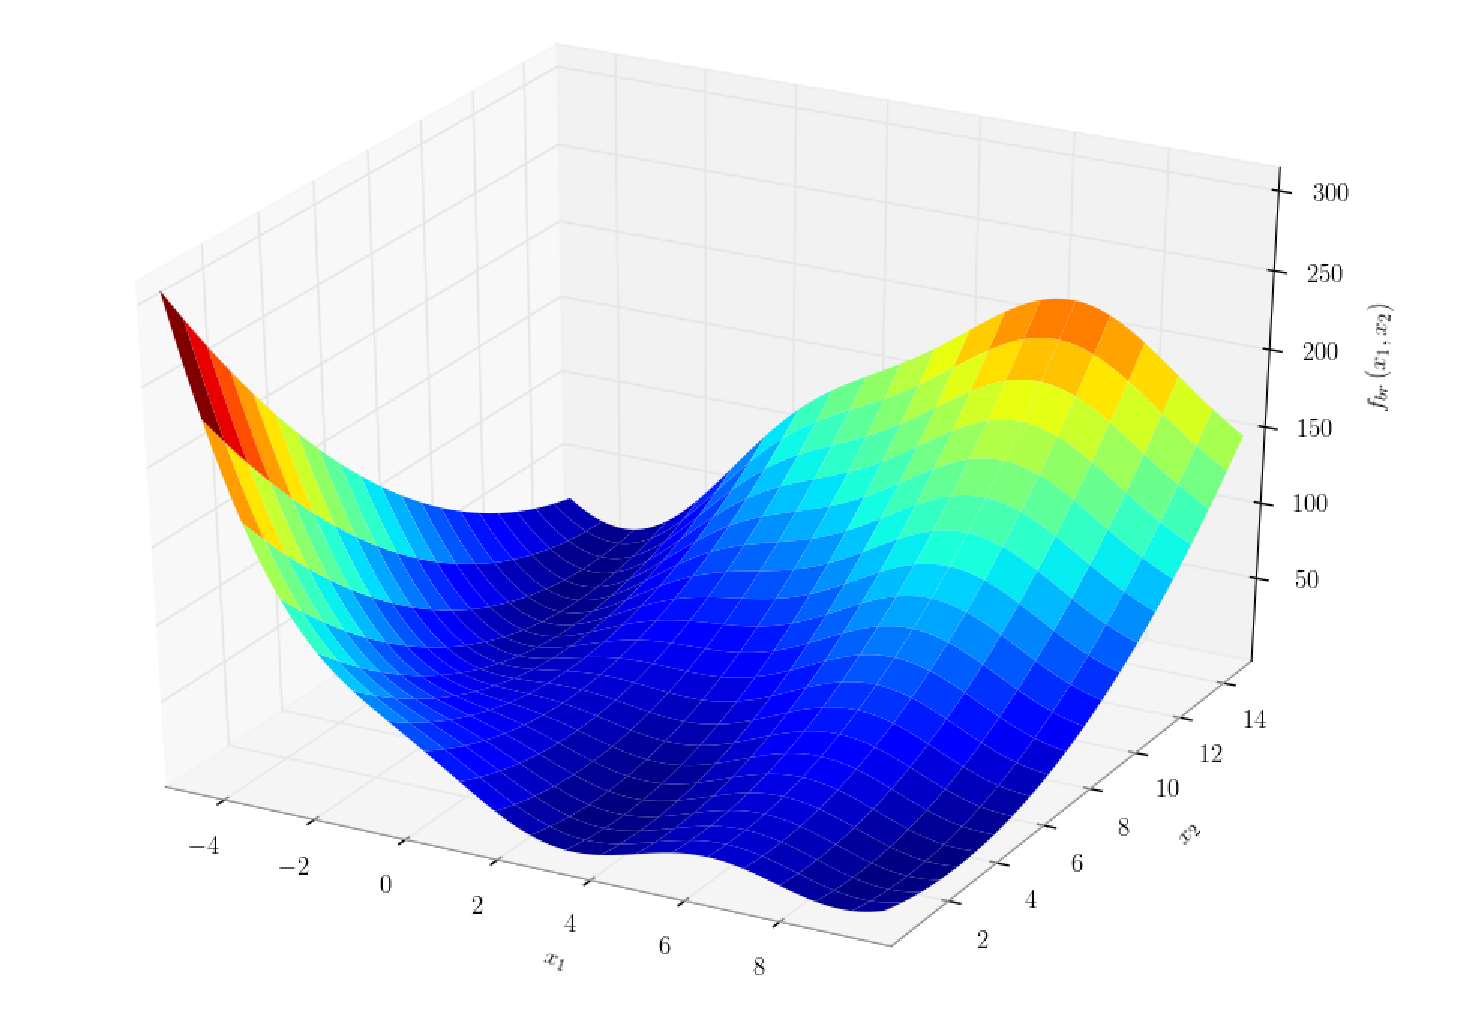
\includegraphics[width=\textwidth]{Chapter5/img/branin.pdf}
    \caption{Branin}
  \end{subfigure}
  \begin{subfigure}{0.33\textwidth}
    \centering\includegraphics[width=\textwidth]{Chapter5/img/himmelblau.pdf}
    \caption{Himmelblau}
  \end{subfigure}
  \begin{subfigure}{0.33\textwidth}
    \centering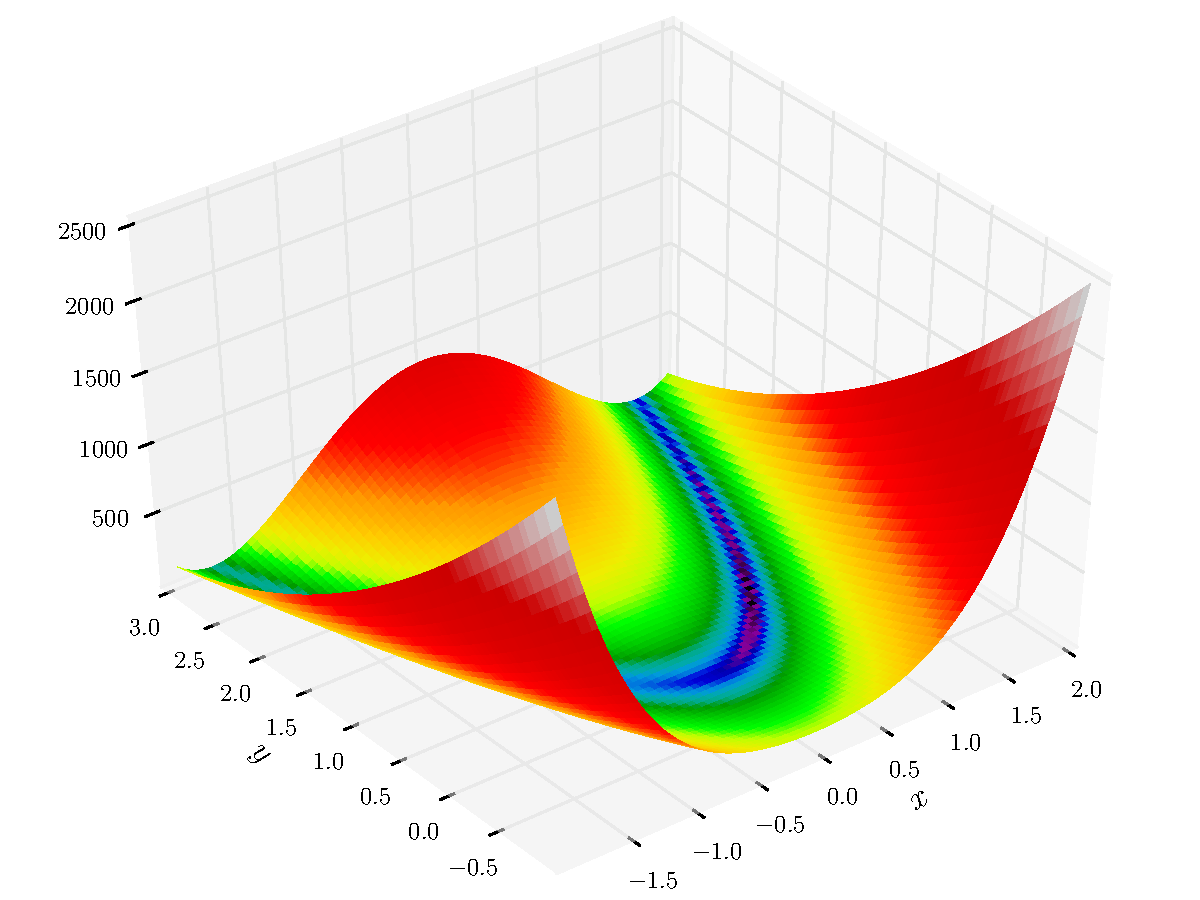
\includegraphics[width=\textwidth]{Chapter5/img/rosenbrock.pdf}
    \caption{Rosenbrock}
  \end{subfigure}
  \begin{subfigure}{0.33\textwidth}
    \centering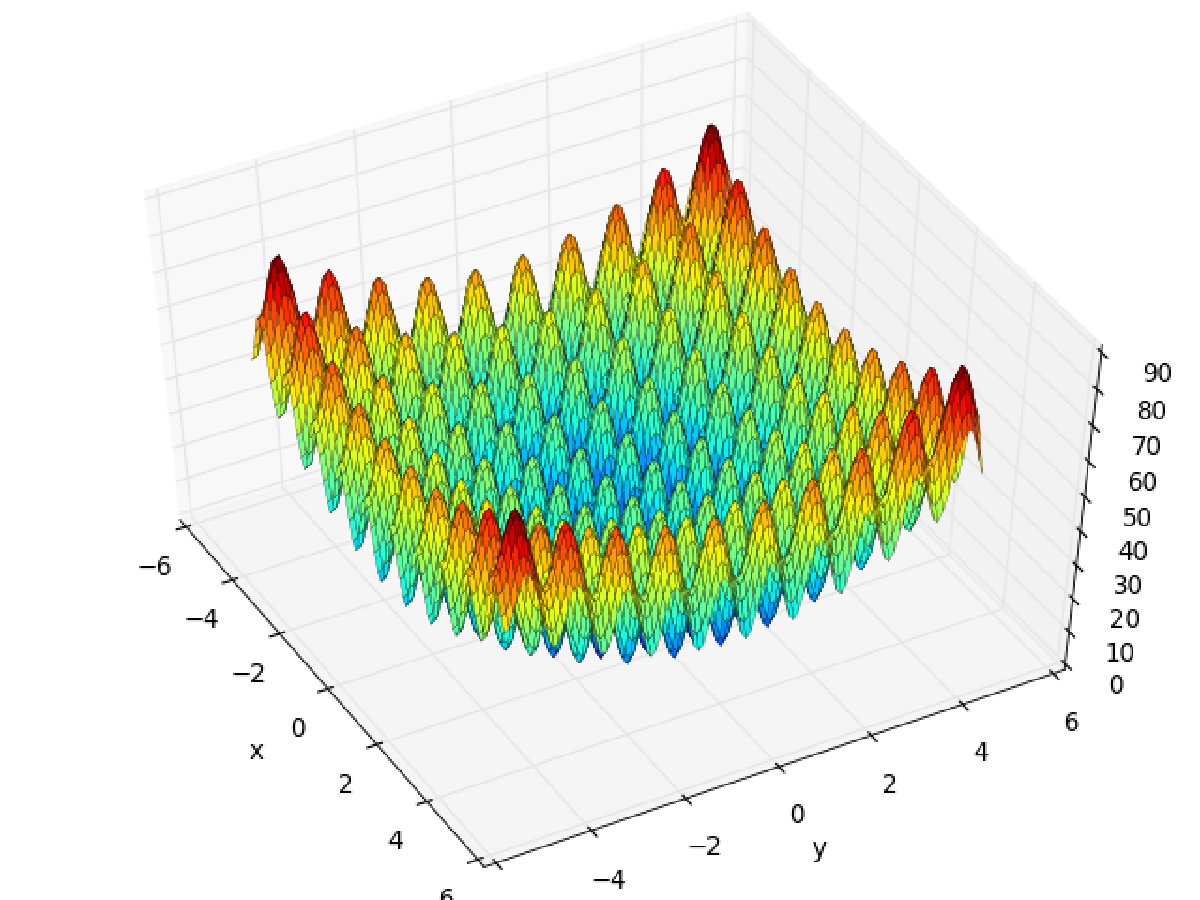
\includegraphics[width=\textwidth]{Chapter5/img/rastrigin.pdf}
    \caption{Rastrigin in 2D}
  \end{subfigure}
  \caption{Benchmark functions for testing black-box optimization algorithms.}
  \label{fig:benchmarks}
\end{figure}

In Figure~\ref{fig:results}, we plot the simple regret of the algorithms as a function of the number of evaluations. All the results are averaged over 5000 runs and we plot the simple regret after 500 function evaluations. Each instance of \gls{hoo} or \gls{hct} would recommend a point picked uniformly at random among those evaluated so that we have the same recommendation strategy as \gls{poo} and \gls{pct}.

\begin{figure}[ht]
  \centering
  \begin{subfigure}{0.33\textwidth}
    \centering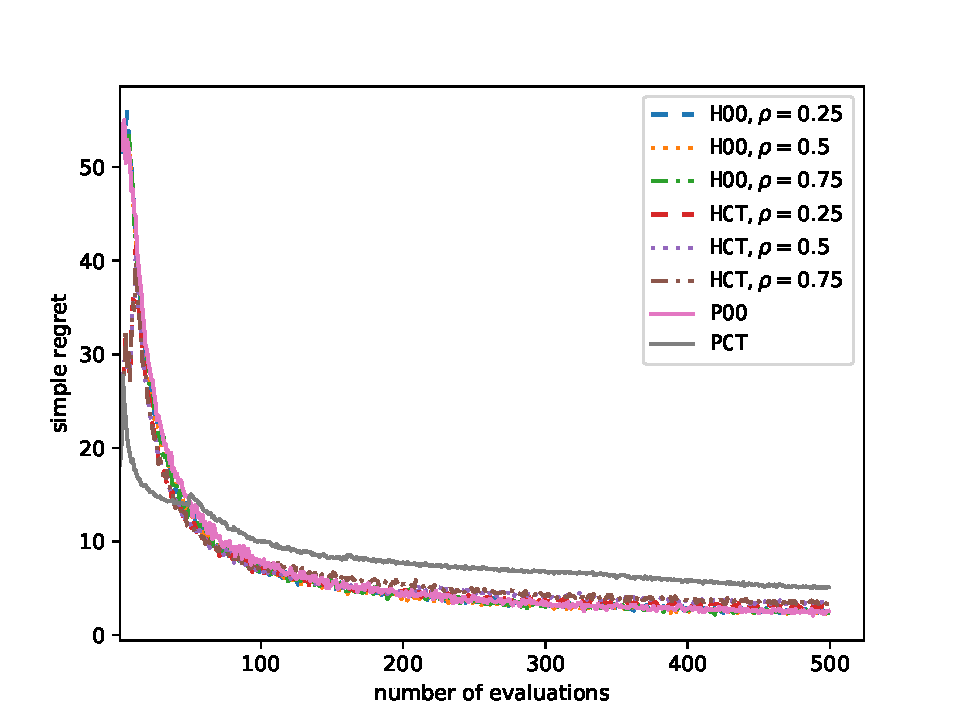
\includegraphics[width=\textwidth]{Chapter5/img/branin_plot.pdf}
    \caption{Branin}
  \end{subfigure}
  \begin{subfigure}{0.33\textwidth}
    \centering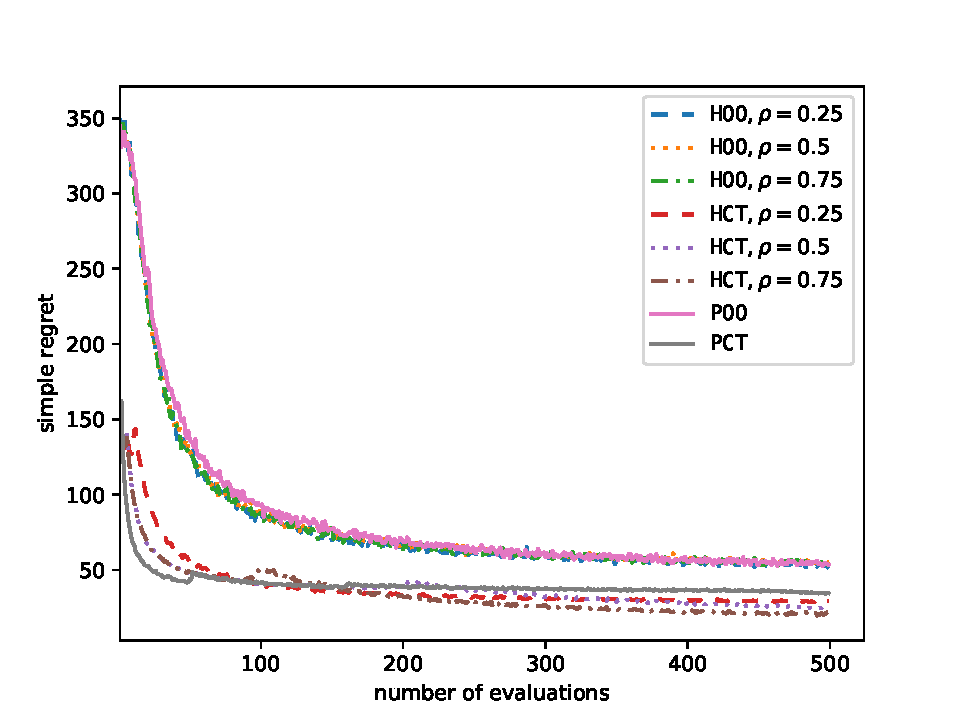
\includegraphics[width=\textwidth]{Chapter5/img/himmelblau_plot.pdf}
    \caption{Himmelblau}
  \end{subfigure}
  \begin{subfigure}{0.33\textwidth}
    \centering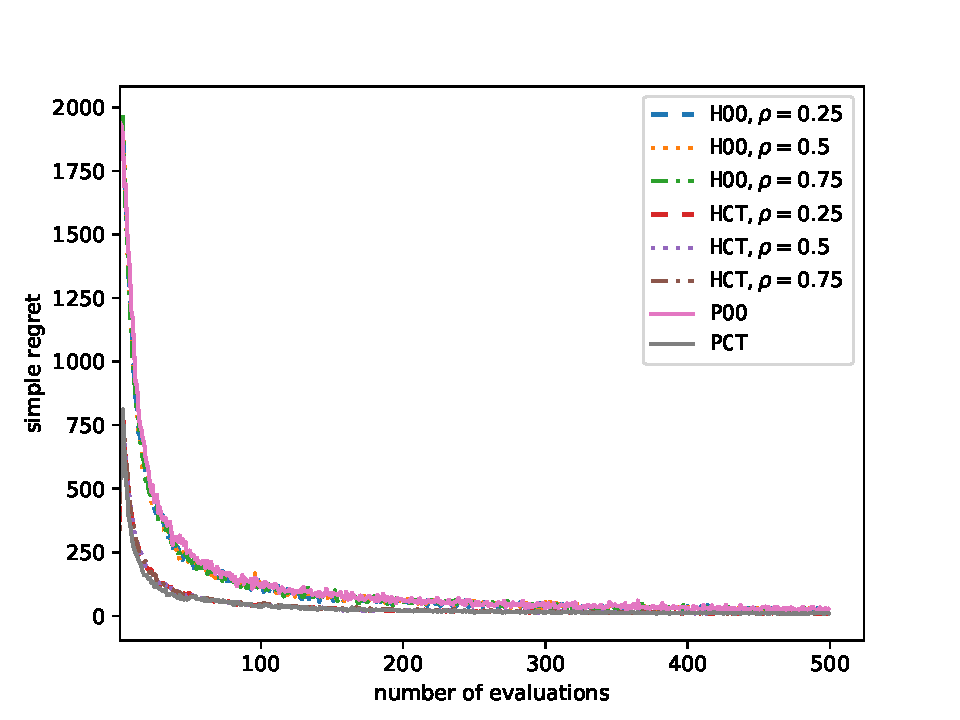
\includegraphics[width=\textwidth]{Chapter5/img/rosenbrock_plot.pdf}
    \caption{Rosenbrock}
  \end{subfigure}
  \begin{subfigure}{0.33\textwidth}
    \centering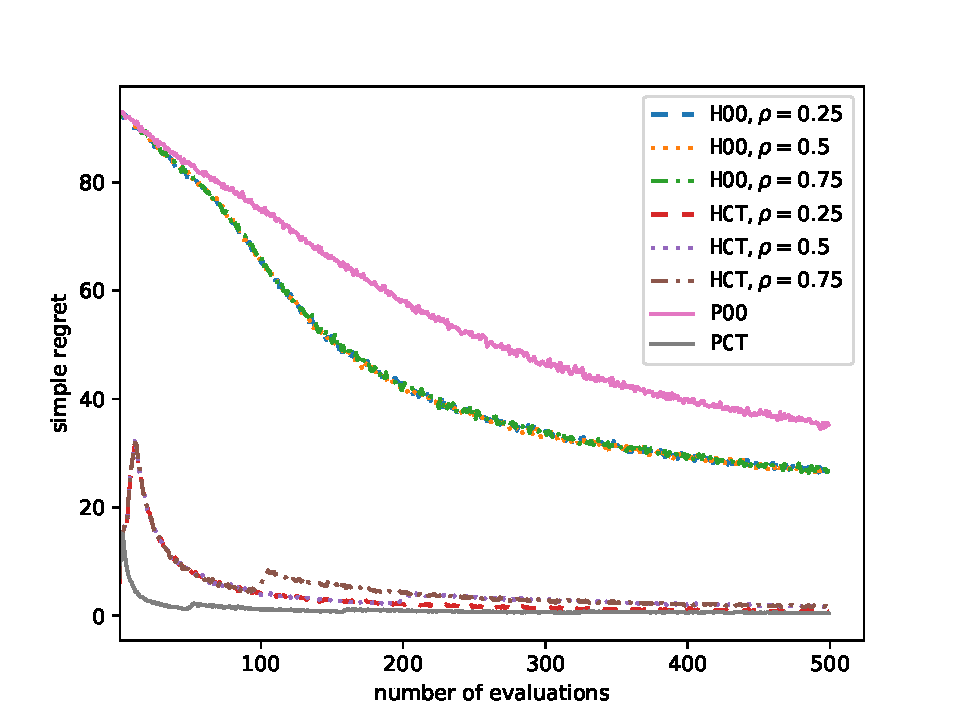
\includegraphics[width=\textwidth]{Chapter5/img/rastrigin_plot.pdf}
    \caption{Rastrigin in 5D}
  \end{subfigure}
  \caption{Simple regret of \POO{} and \PCT{} run for different $\rho$ values.}
  \label{fig:results}
\end{figure}

The first observation is that \gls{pct} does match the performance of some single \gls{hct} instances as expected. We also notice that \gls{pct} has comparable performance w.r.t.\,\gls{poo} in these plots, which justifies the choice of using \gls{hct} as a subroutine for the \gls{poo} meta-algorithm.


% !TEX root = ../Chapter5.tex
\section{Discussion}\label{sec:gpo.discussion}

We studied \PCT, a new instantiation of \POO on top of \HCT. We proved that \HCT is a plausible subroutine for \POO by adapting the analysis of \HCT under a new assumption w.r.t.\,a fixed partitioning. We also proposed \GPO, a general framework for making any hierarchical bandit algorithm that only has a simple regret guarantee adaptive to unknown smoothness. However, whether it is possible to weaken the assumptions of \HOO in the same way as \HCT while keeping similar regret guarantees remains open.


% Manual newpage inserted to improve the layout of sample file - not
% needed in general before appendices/bibliography.

% \newpage
% \bibliographystyle{plainnat}
% \bibliography{Major,Minor}
% \newpage


	%%%%%%%%%%%%%%%%%%%%%%%%%%%%%%%%%%%%%%%%%%%%%%%%%%%%%%%%%%%%%%%%%%%%%%%%%%%%%%%%%%%%%%%%%%%%%%
%%									Chapitre 6												%
%%%%%%%%%%%%%%%%%%%%%%%%%%%%%%%%%%%%%%%%%%%%%%%%%%%%%%%%%%%%%%%%%%%%%%%%%%%%%%%%%%%%%%%%%%%%%

\chapter{Bandits and Hyper-Parameter Optimization}\label{CHAP:DTTTS}
	\citationChap{
		True optimization is the revolutionary contribution of modern search to decision processes.
	}{George Dantzig}
	\minitoc
	\newpage

%%%%%%%%%%%%%%%%%%%%%%%%%%%%%%%%%%%%%%%%%%%%%%%%%%%%%%%%%%%%%%%%%%%%%%%%%%%%%%%%%%%%%%%%%%%%%



% Début du chapitre
\addtocontents{toc}{\protect\setcounter{tocdepth}{1}}
\section{Introduction}\label{sec:dttts.intro}

Training a machine learning algorithm often requires to specify several parameters. For instance, for neural networks, it is the architecture of the network and also the parameters of the gradient algorithm used or the choice of regularization. These \gls{hyper-parameters} are difficult to learn through the standard training process and are often manually specified.
%\todo{some ref so this is not just blabla}

When it is not feasible to design algorithms with a few hyper-parameters, we opt for \gls{hpo}. \gls{hpo} is a crucial component of modern machine learning and \gls{automl}. Recall that \gls{hpo} can be viewed as a \gls{bbo}/\gls{go} problem (see Chapter~\ref{sec:intro.mab.hpo}) where the evaluation of the objective function is expensive as it is the accuracy of a learning algorithm for a given configuration of hyper-parameters. Indeed, a typical function evaluation involves training the primary machine learning algorithm to completion on a dataset, which often takes a considerable amount of time or resources, in particular for large \gls{dl} models. For example, the training of language representation model \texttt{BERT-Large}~\citep{devlin2019bert} was performed on 16 Cloud TPUs (64 TPU chips in total), and each pre-training took 4 days to complete. This vastly limits the number of evaluations that can be carried out, which calls for a design of efficient high-level algorithms that automate the tuning procedure.

In this chapter, we are interested in exploring how \gls{mab}, or more precisely \gls{bai}, can guide the design of efficient \gls{hpo}. Indeed, some bandit tools have already been employed for \gls{go} (see Chapter~\ref{CHAP:GPO}) and \gls{hpo}: First, in the field of Bayesian optimization, the \GPUCB algorithm \citep{srinivas2010gpucb} is a Gaussian process extension of the classical \UCB bandit algorithm~\citep{auer2002ucb}. Later, \citet{hoffman2014bayesgap} proposed to use \gls{bai} tools -- still with a Bayesian flavor -- for automated machine learning, where the goal is to smartly try hyper-parameters from a pre-specified \emph{finite} grid. 

However, in most cases, the number of hyper-parameter configurations to explore is infinite. In this chapter, we investigate the use of bandit tools suited for an \emph{infinite} number of arms. There are two lines of work for tackling a very large or infinite number of configurations (arms). The first is the continuum-armed bandits discussed in Chapter~\ref{CHAP:GPO} (see also~\citealt{bubeck2010x,grill2015poo,shang2019adaptive,bartlett2019simple}). It makes use of hierarchical bandit tools and aims at exploiting the (possibly unknown) smoothness of the black-box function to optimize. To the best of our knowledge, these methods have never been extensively tested in practice for \gls{hpo}.

The second line of work does not assume any smoothness: At each round, the learner may ask for a new arm from a \gls{reservoir} distribution $\nu_0$ (pick randomly a new hyper-parameter configuration) and add it to the current arm pool $\cX$, or re-sample one of the previous arms (evaluate configuration already included in $\cX$), in order to find an arm with a good mean reward (i.e., a hyper-parameter configuration with a good validation accuracy). It is the \gls{infinitely-armed bandits} setting. In particular, we study the stochastic case in which observations are assumed to be independent. The \gls{siab} is studied by \citet{berry1997infinite,wang2008ucbv} for the rewards maximization problem while \citet{carpentier2015siri,aziz2018confidence} study the simple regret problem, which is related to \gls{bai}. While most proposed algorithms consist of querying an \emph{adequate} number of arms from the reservoir before running a standard BAI algorithm, \cite{li2017hyperband} propose a more robust approach called \Hyperband{} that uses several such phases.

\paragraph{Contributions.}
\textbf{1)}
In this chapter, we go even further and propose the first \emph{dynamic} algorithm for BAI in SIAB, that at each round, may either query a new arm from the reservoir or re-sample arms previously queried. Our algorithm leverages a Bayesian model and builds on \gls{ttts}. 
\textbf{2)}
We also introduce a variant of \Hyperband{} where the \SHA subroutine~\citep{karnin2013sha} is replaced by \gls{ttts}. 
\textbf{3)}
Numerical studies are presented to show the competitiveness and robustness of the proposed dynamic algorithm with respect to state-of-the-art \gls{hpo} methods.
%\todo{cut this in space needed}
%\paragraph{Outline} We first introduce a general framework for hyper-parameter optimization in Section~\ref{sec:framework}. In Section~\ref{sec:bai}, we explain how infinitely-many armed bandit algorithms can be used for \gls{hpo}, before presenting our two new algorithms in Section~\ref{sec:algo}. Finally, we provide experimental results in Section~\ref{sec:result}. % before concluding.


\section{A Brief Survey of Automated Machine Learning}\label{sec:dttts.survey}

We provide a full-stack pipeline for a machine learning procedure as displayed in Fig.~\ref{fig:automl} and a general taxonomy on different components of AutoML~\citep{hutter2019automl,zoller2019automl,he2019automl}. We pay particular attention to hyper-parameter optimization, neural architecture search and meta learning later in separate subsections. The following structure is partly inspired by various surveys mentioned in the references.

\begin{figure}[ht]
    \centering
    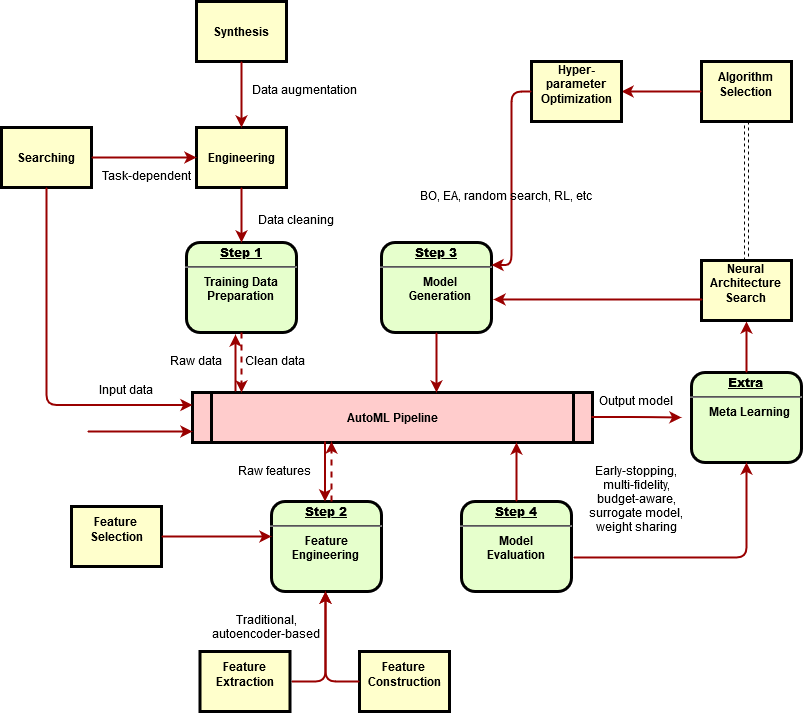
\includegraphics[width=\textwidth]{Chapter6/img/automl.png}
    \caption{The full-stack pipeline of a machine learning task.}
    \label{fig:automl}
\end{figure}


\subsection{The AutoML taxonomy}\label{sec:dttts.survey.taxonomy}

\paragraph{Data preparation}

\begin{itemize}
    \item Data collection
    \begin{itemize}
        \item Web searching, however data could be ill-labeled or inaccurate, semi-supervised or self-labeling methods are required;
        \item Data synthesis when not enough data available, mainly using data augmentation.
    \end{itemize}
    \item Data cleaning
    \begin{itemize}
        \item Standardization;
        \item Scaling;
	    \item Binarization of numerical (discrete or continuous) attributes;
	    \item One-hot encoding for categorical attributes;
	    \item Imputation (e.g. with mean values).
    \end{itemize}
    \item Feature engineering
\end{itemize}

\paragraph{Feature engineering}

\begin{itemize}
    \item Feature selection
    \begin{itemize}
        \item Subset generation, using some (random) search strategy (simulated annealing, genetic algorithms);
        \item Subset evaluation with filter methods, wrapper methods or embedded methods (deep learning, decision trees, etc);
        \item Subset validation.
    \end{itemize}
    \item Feature extraction (alters the features)
    \begin{itemize}
        \item Dimensionality reduction techniques like PCA, ICA, LDA, etc;
        \item Autoencoder-based methods.
    \end{itemize}
    \item Feature construction
    \begin{itemize}
        \item Searching methods such as tree-based approaches, genetic algorithms;
        \item Annotation-based approaches.
    \end{itemize}
\end{itemize}

\paragraph{Pipeline generation} 
This is the most important part to be further detailed.

\begin{itemize}
    \item FMS (full model selection) or CASH (combined algorithm and hyper-parameter optimization)
    \begin{itemize}
        \item Model/Algorithm selection;
        \item HPO (hyper-parameter optimization).
    \end{itemize}
    \item NAS (neural architecture search)
    \item Ensembling, since choosing one single full model maybe a waste
    \item Metal learning
\end{itemize}

\paragraph{Model evaluation or estimation}

\begin{itemize}
    \item Complete training (time and resource-consuming especially)
    \item Multi-fidelity (low resolution, subset of data, not only for DL)
    \item Early-stopping (mostly for DL)
    \item Surrogate model (not only for DL)
    \item Weight sharing (DL-specific)
    \item Resource/budget-aware (computational cost is added to the loss)
\end{itemize}
    
    
\paragraph{Existing (open source) AutoML frameworks} 
TPOT, AutoKeras, auto-sklearn, Transmogrif, MLBox

\subsection{Hyper-parameter optimization}\label{sec:dttts.survey.hpo}

\paragraph{Black-box optimization}

\begin{itemize}
    \item Model-free
    \begin{itemize}
        \item \Random, \Grid;
        \item Population-based as \CMAES, more precisely genetic algorithms, evolutionary algorithms, evolutionary strategies, and particle swarm optimization: maintain a population, then improve this population by applying mutations or crossovers.
    \end{itemize}
    \item Model-based (in particular Bayesian optimization)
    \begin{itemize}
        \item Traditional Bayesian optimization with various surrogate models and acquisition functions, like \GPUCB, \PI, \EI with Gaussian processes and \SMAC with random forests; 
        \item Atypical Bayesian optimization \TPE;
        \item Thompson sampling-based \DTTTS.
    \end{itemize}
\end{itemize}

\paragraph{Gray-box optimization}

\begin{itemize}
    \item Multi-fidelity Optimization
    \begin{itemize}
        \item Bandit-based algorithm \Hyperband, that introduces the concept of partial training;
        \item `Auto-WEKA` appears to be the only paper that uses only one or a few of the cross-validation folds;
        \item Bayesian optimization + partial training = \BOHB;
        \item Learning curve.
    \end{itemize}
    \item Gradient-based
\end{itemize}

% - Current Benchmark (they are mostly designed for a continuous search space)
%     - `Random Search`
%     - `CMA-ES`
%     - `SMAC`
%     - `TPE`
%     - `Hyperband`
%     - `BOHB`

\subsection{Meta learning}\label{sec:dttts.survey.meta}

\subsection{Neural architecture search}\label{sec:dttts.survey.nas}

\paragraph{Model generation}

\begin{itemize}
    \item Elemental operations
    \begin{itemize}
        \item Convolution;
        \item Pooling (max-pooling, average-pooling, attention);
        \item Concatenation;
        \item Addition;
        \item Skip connection (ResNet).
    \end{itemize}
    \item Model structures
    \begin{itemize}
        \item Entire structure;
        \item Cell-based structure (normal cell or reduction cell like `NASNet`): internal cell design with human-designed operations;
        \item Progressive structure;
        \item Morphism-based structure.
    \end{itemize}
\end{itemize}

\paragraph{Hyper-parameter Optimization}

\begin{itemize}
    \item Classical HPO methods
    \item RL-based methods
\end{itemize}


\section{Hyper-Parameter Optimization Framework}\label{sec:dttts.framework}

In this chapter, we view \gls{hpo} as a particular \gls{go} setting, for which the target function $f$ is a mapping from a hyper-parameter configuration to some measure of failure for the machine learning algorithm trained with these hyper-parameters. Formally, we aim at solving an optimization problem of the form 
\[
f^\star = \min \left\{f(\blambda):\blambda\in\Omega\right\}\,,
\]
where $\blambda$ denotes a configuration of hyper-parameters chosen from a configuration space $\Omega$. A hyper-parameter optimizer is a sequential procedure, that at each round $n$, selects a configuration~$\blambda_n$ to evaluate using some sampling rule, after which a (costly and \emph{noisy}) evaluation of $f(\blambda_n)$ is observed. Besides, a hyper-parameter configuration $\hat{\blambda}^\star$ is recommended as a guess for a close-to-optimal configuration at the end. The hope is that $f(\hat{\blambda}^\star)$ is not far from $f^\star$.

We restrict our attention to hyper-parameter tuning for supervised learning algorithms. Given a training dataset $\cD_{\texttt{train}}$ containing $m$ labeled examples in $\cX \times \cY$ and a choice of hyper-parameter configuration $\blambda$, a supervised learning algorithm (neural network, \SVM, gradient boosting, \dots) produces a predictor $\hat{g}_{\bm\lambda}^{\,(m)}\!:\cX \rightarrow \cY$. Note that there can be some randomness in the training process (e.g., if stochastic gradient descent is used) so that $\hat{g}_{\blambda}^{\,(m)}$ may still be random for a given training set and hyper-parameters. The goal is to build a predictor that generalizes well. If we had access to the distribution $\bP$ that generated the data (i.e., assuming that data points in $\cD_{\texttt{train}}$ are i.i.d. from $\bP$), this generalization power would be measured by the risk $f(\bm\lambda) \triangleq \mathbb{E}\left[\ell\left(\bm Y,\hat g_{\blambda}^{\,(m)}(\bm X)\right) \right]$, where $\ell$ is some loss function measuring the distance between two predictions and the expectation is taken on $(\bm X , \bm Y) \sim \bP$ and the possible randomness in the training process. 


% Given a set of hyper-parameters $\blambda$, the objective of a (supervised) learning process is to train a model $g_{\blambda}:\cX\lra\cY$ that minimizes the total empirical loss (could be regularized) over a training set $\cD_{\texttt{train}} = \{(\bx_i,\by_i)_{i=1, \ldots, |\cD_{\texttt{train}}|}\}$ where $(\bx_i,\by_i)\in\cX\times\cY$ are pairs of input and output,
% \[
% 	\cL_{\texttt{train}}(\blambda) \eqdef \sum_{i=1}^{|\cD_{\texttt{train}}|} \ell_1(g_{\blambda}(\bx_i),\by_i).
% \]
% Here the loss function $\ell_1$ should be neatly chosen for a specific task.
% 
% In the context of hyper-parameter tuning, our objective is then to minimize the following black-box function
% \[
%     f(\blambda) \eqdef \EE{\mathbb{P}_{\bx,\by\sim \cD_{\texttt{valid}}}\left[\by\neq\hat{g}_{\blambda}(\bx)\right]},
% \]
% where the randomness of the expectation comes eventually from the training set that we are using. 

In practice, however, the explicit evaluation of $f$ is impossible, but there are several methods for \emph{noisy evaluations}. We can either compute the validation error of $\hat g_{\blambda}^{\,(n)}$ on a held-out validation set,  
\[
    \frac{1}{|\cD_{\texttt{valid}}|} \sum_{i=1}^{|\cD_{\texttt{valid}}|} \ell(\hat{g}^{\,(m)}_{\blambda}(\bx_i),\by_i)\,,
\]
or a cross validation error over the training set as an approximation of the  objective. %We specify this loss function for real hyper-parameter optimization tasks in Section~\ref{sec:result}.


\section{Best-Arm Identification for Hyper-Parameter Tuning}\label{sec:dttts.bai}

Hyper-parameter optimization can be modeled as a BAI game. Given a finite set of arms $\cX \eqdef \{1,\ldots,K\}$, when we select arm $i$, we get an independent observation from some unknown distribution $\nu_i$ with mean $\mu_i$. A BAI algorithm sequentially selects arms in order to identify the arm with the largest mean\footnote{Here we present BAI problems in a standard way for which we search for an arm with the largest mean. For \gls{hpo}, however, it is important to mention that we are searching for a hyper-parameter configuration that minimizes the validation error. One can easily see that it does not change the problem in principle.}, $I^\star \eqdef \argmax_{i\in\cA}\mu_i$. 

In the context of \gls{hpo}, each arm models the quality of a given hyper-parameter configuration $\bm\lambda$. When the arm is sampled, a noisy evaluation of $f(\bm\lambda)$ is received, which is the mean reward of that arm.

%Recall that a fixed-budget BAI (or pure-exploration) algorithm consists of a sequential arm selection strategy, indicating which arm $I_n$ is selected at round $n$, coupled with a decision that selects a candidate best arm ${I}^\star_n$ at round $n$. The goal is either to minimize the error probability $\bP(\mu_{{I}^\star_n}\neq\mu_{I^\star})$ \citep{audibert2010budget,karnin2013sha} or the \emph{simple regret}~\citep{bubeck2009pure,gabillon2012ugape}, defined as $r_t = \mu_{I^\star} - \mu_{{I}^\star_t}$, possibly after a total budget $B$, whose knowledge may be used by the algorithm. Note that the BAI problem can also be studied from a fixed-confidence point of view \citep{even-dar2003confidence}. 

As stated in Section~\ref{sec:dttts.intro}, standard \gls{bai} algorithms are not straightforwardly applicable to \gls{hpo} when the search space can be infinite and is often continuous. To handle such cases, we rather turn our attention to \gls{siab}. In this context, there is an infinite pool of arms, whose means are assumed to be drawn from some \gls{reservoir} distribution $\nu_0$. In such a model, a BAI algorithm maintains a list of arms that have been tried before. At each round it can either query a new arm from the reservoir, add it to the list and sample it, or sample an arm already in the list.

A natural way to perform BAI in an infinite-many armed bandit model consists of first querying a \emph{well-chosen} number of arms from the reservoir and then running a standard BAI algorithm on those arms~\citep{carpentier2015siri}. However this ideal number may rely on the difficulty of the learning task, which is hardly known in practice. The \Hyperband{} algorithm \citep{li2017hyperband} takes a step further and successively queries several batches of arms from the reservoir, including a decreasing number of arms in each batch, while increasing the budget dedicated to each of them. \SHA \citep{karnin2013sha}, a state-of-the-art fixed-budget \gls{bai} algorithm, is then run on each of these batches of arms. This approach seems more robust in that it trades off between \emph{the number of arms that is needed to capture a good arm} and \emph{how much measurement effort we should allocate to each of them}. However, a numerical study performed by \cite{aziz2018infinite} seems to reveal that an infinite bandit algorithm based on \SHA should always query the maximal number of arms from the reservoir\footnote{This reference is a preliminary draft that has been withdrawn due to technical issues in the proofs. Yet we believe the experimental section to be sound.}. 

In Table~\ref{table:hpo}, we summarize how to cast \gls{hpo} as a \gls{bai} problem with infinitely-many arms.

\begin{table}[ht]
\centering
\def\arraystretch{1.5}
\begin{tabular}[r]{|c|c|} \hline
\textbf{\texttt{BAI}} & \textbf{\texttt{HPO}}\\
\hline
query $\nu_0$ & \ pick a new configuration $\blambda$\.\ \\
\hline
\ sample an arm\. & train the classifier $g_{\blambda}$ \\
\hline
reward & cross-validation loss \\
\hline
\end{tabular}
\caption{Casting HPO as a BAI problem.}
\label{table:hpo}
\end{table}


All existing algorithms are still subject to a pre-defined scheduling of how many arms should be queried from the reservoir. The algorithm (\DTTTS) we propose in next section does not need to decide in advance how many arms will be queried, and is therefore fully \emph{dynamic}. %The algorithm is inspired by a variant of Thompson sampling~\citep{thompson1933} called Top-Two Thompson sampling (\TTTS,~\citealt{russo2016ttts}). 

\begin{remark}
\begin{leftbar}[remarkbar]
\Hyperband is proposed specifically for hyper-parameter tuning. Its original philosophy is to adaptively allocate \emph{resources} to more promising configurations. Resources here can be time, dataset sub-sampling, feature sub-sampling, etc. In such a setting, the classifier is not always trained into completion given a parameter configuration, but is rather stopped early if it is shown to be bad so that we can allocate more resources to other configurations. In this case, different evaluations of a single configuration cannot be considered as i.i.d. anymore. Thus, \gls{hpo} is stated as a non-stochastic infinitely-armed bandit problem. This idea of early stopping is also further investigated by combining Bayesian optimization with it~\citep{falkner2018bohb}. However, this is about the model evaluation of Section~\ref{sec:dttts.survey.hpo} and is out of the scope of this thesis.
\end{leftbar}
\end{remark}


\section{Active \TTTS{} for Hyper-Parameter Optimization}\label{sec:dttts.algorithm}

In this section, we introduce a new algorithm for \gls{bai} in an infinite bandit model, that is an adaptation of \gls{ttts}{} (see Chapter~\ref{CHAP:T3C}). Unlike \SHA{} that requires the knowledge of the total budget to operate, \gls{ttts}{} is particularly appealing as it does not need to have it. Remember that such algorithms are referred to as \emph{anytime}. Besides, it is known to be optimal in a Bayesian (asymptotic) sense (see Chapter~\ref{CHAP:T3C}).

Recall that as a Bayesian algorithm, \gls{ttts} uses a prior distribution $\Pi_0$ over the vector of means of the $K$ arms, $\bmu \triangleq (\mu_1,\cdots,\mu_K)$, which can be updated to a posterior distribution $\Pi_n$ after $n$ observations. 

We consider Bernoulli bandit model in the rest of this chapter. Under Bernoulli bandit model, arm $i$ produces a reward $r_{n,i}=1$ with probability $\mu_i$, and $r_{n,i}=0$ with probability $1-\mu_i$ when sampled at round $n$. Given independent uniform prior for the mean of each arm, the posterior distribution on $\bmu$ is a product of $K$ Beta distributions: $\Pi_n = \bigotimes_{i=1}^{K} \texttt{Beta}(1+S_{n,i},N_{n,i}-S_{n,i}+1)$, where $N_{n,i}$ is the number of selections of arm $i$ until round $n$ and $S_{n,i}$ is the sum of rewards obtained from that arm. 
%At each round $n$, \gls{ttts} chooses one arm from the following two candidates to evaluate: (1) it first samples a parameter ${\bm\theta}$ from $\Pi_{t-1}$, and the first candidate is defined as $I_n^{\,(1)} \eqdef \argmax_{i\in\cX} {\theta}_i$, (2) it repeatedly samples new ${\bm\theta}'$ until $I_n^{\,(2)} \eqdef \argmax_{i\in\cX} \theta_i'$ is different from $I_n^{\,(1)}$. \gls{ttts} depends on a parameter $\beta \in (0,1)$. In particular, the algorithm selects $I_n = I_n^{\,(1)}$ with probability $\beta$ and $I_n = I_n^{\,(2)}$ with probability $1-\beta$.

\paragraph{Best of best-arm identification.}

We further motivate experimentally why we choose to build new algorithms upon \gls{ttts} in this section. 

We consider here some fixed-budget and anytime \gls{bai} algorithms, including uniform allocation~\citep{bubeck2009pure}, \UCBE{} and \SR{}~\citep{audibert2010budget}, \UGapE~\citep{gabillon2012ugape}, \SHA{}, \TS{} with a MPA strategy of decision (see Section~\ref{sec:mab.bai.decision}), \gls{ttts}{}, \ATLUCB{}~\citep{jun2016atlucb}.

We use 8 problem instances proposed by~\cite{audibert2010budget}, all settings consider Bernoulli bandits, and we compare their trending \emph{simple regret} averaged on 1000 trials. The results are shown in Fig.~\ref{fig:bai}.

\begin{itemize}
	\item Setting 1: $\mathbf{\mu_1}=0.5, \mathbf{\mu_{2:20}}=0.4, \operatorname{budget}=2000$
	\item Setting 2: $\mathbf{\mu_1}=0.5, \mathbf{\mu_{2:6}}=0.42, \mathbf{\mu_{7:20}}=0.38, \operatorname{budget}=2000$
	\item Setting 3: $\mathbf{\mu}=[0.5, 0.3631, 0.449347, 0.48125839], \operatorname{budget}=2000$
	\item Setting 4: $\mathbf{\mu}=[0.5, 0.42, 0.4, 0.4, 0.35, 0.35], \operatorname{budget}=600$
	\item Setting 5: $\mathbf{\mu_1}=0.5, \mathbf{\mu_i}=\mathbf{\mu_1}-0.025i, \forall i\in\{2\ldots15\}, \operatorname{budget}=4000$
	\item Setting 6: $\mathbf{\mu_1}=0.5, \mathbf{\mu_2}=0.48, \mathbf{\mu_{3:20}}=0.37, \operatorname{budget}=6000$
	\item Setting 7: $\mathbf{\mu_1}=0.5, \mathbf{\mu_{2:6}}=0.45, \mathbf{\mu_{7:20}}=0.43, \mathbf{\mu_{7:20}}=0.38, \operatorname{budget}=6000$
	\item Setting 8: $\mathbf{\mu_1}=0.5, \mathbf{\mu_{2:6}}=0.45, \mathbf{\mu_{7:20}}=0.43, \mathbf{\mu_{7:20}}=0.38, \operatorname{budget}=12000$
\end{itemize}

\begin{figure}[ht]
  \centering
  \begin{subfigure}[t]{0.25\textwidth}
    \centering\includegraphics[width=\textwidth]{Chapter6/img/bai/setting1.png}
    \caption{Problem 1}
  \end{subfigure}%
  \begin{subfigure}[t]{0.25\textwidth}
    \centering\includegraphics[width=\textwidth]{Chapter6/img/bai/setting2.png}
    \caption{Problem 2}
  \end{subfigure}
  \begin{subfigure}[t]{0.25\textwidth}
    \centering\includegraphics[width=\textwidth]{Chapter6/img/bai/setting3.png}
    \caption{Problem 3}
  \end{subfigure}%
  \begin{subfigure}[t]{0.25\textwidth}
    \centering\includegraphics[width=\textwidth]{Chapter6/img/bai/setting4.png}
    \caption{Problem 4}
  \end{subfigure}
  \begin{subfigure}[t]{0.25\textwidth}
    \centering\includegraphics[width=\textwidth]{Chapter6/img/bai/setting5.png}
    \caption{Problem 5}
  \end{subfigure}
  \begin{subfigure}[t]{0.25\textwidth}
    \centering\includegraphics[width=\textwidth]{Chapter6/img/bai/setting6.png}
    \caption{Problem 6}
  \end{subfigure}
  \begin{subfigure}[t]{0.25\textwidth}
    \centering\includegraphics[width=\textwidth]{Chapter6/img/bai/setting7.png}
    \caption{Problem 7}
  \end{subfigure}
  \begin{subfigure}[t]{0.25\textwidth}
    \centering\includegraphics[width=\textwidth]{Chapter6/img/bai/setting8.png}
    \caption{Problem 8}
  \end{subfigure}
  \caption{Comparing different fixed-budget and anytime BAI algorithms.}
  \label{fig:bai}
\end{figure}

In these experiments, \gls{ttts} are always beating or at least performing as well as its competitors. It thus seems to be a good candidate to be further investigated.

Note that \gls{ttts} can also be used for bandit settings in which the rewards are bounded in $[0,1]$ by using a binarization trick first proposed by~\cite{agrawal2012analysis}: When a reward $r_{n,i} \in [0,1]$ is observed, the algorithm is updated with a fake reward  
\[
    r'_{n,i} \sim \texttt{Bern}(r_{n,i}) \in \{0,1\}\,.
\]
\gls{ttts} can thus be used for \gls{bai} for a \emph{finite} number of arms that with rewards in $[0,1]$. We now present a simple way of extending \gls{ttts}{} to deal with an infinite number of arms, namely \gls{dttts}.

\paragraph{Dynamic \TTTS{}.}

%The rationale behind \DTTTS is the following. 

In an infinite bandit algorithm, at each round, we either query a new arm from the reservoir \emph{and sample it}, or re-sample a previous arm. In a Bayesian setting, we can also imagine that at each round, an arm is queried from the reservoir and added with a \textit{uniform prior} to the list of queried arms, \emph{regardless of whether it is sampled or not}. Then, at round $t$, \DTTTS consists in running \gls{ttts} on these $t$ arms, out of which several are endowed with a uniform prior and have never been sampled. 

Leveraging the fact the the maximum of $k$ uniform distribution has a \texttt{Beta}($k,1$) distribution and that \gls{ttts} only depends on the maxima of posterior samples, we give the following equivalent implementation for \DTTTS (Algorithm~\ref{alg:dttts}). Letting $\cL_n$ be the list of arms that have been queried  from the reservoir and sampled \textit{at least once} before round $t$, at round $t$ we run \gls{ttts} on the set $\cX_n \triangleq \cL_n \cup \{\mu_0\}$ where $\mu_0$ is a pseudo-arm with posterior distribution \texttt{Beta}($n-k_n, 1$), where $k_n\triangleq|\cL_n|$.  

\begin{algorithm}[ht]
\centering
\caption{Sampling rule of Dynamic \DTTTS{}}
\label{alg:dttts}
\begin{algorithmic}[1] %[1] enables line numbers
    \State {\bfseries Input: } $\beta$; $B$ (total budget); $\nu_0$
    \State {\bfseries Initialization: } $\mu_1 \sim \nu_0$; $t \gets 0$; $\cX \gets \{\mu_0,\mu_1\}$; $m\gets1$; $S_0, N_0 \gets 0$; $S_1 \sim \texttt{Bern}(\mu_1)$, $N_1 \gets 1$\
    
    \While{$n < B$}
	    \State $\forall i=0,\dots,m$, $\theta_i \sim \texttt{Beta}(S_i+1,N_i-S_i+1)$; $U \sim \cU([0,1])$
	    \State $I^{\,(1)} \gets \argmax_{i=0,\dots,m} \theta_i$
	    \If{$U > \beta$}
	        \While{$I^{\,(2)} = I^{\,(1)}$} 
	            \State $\forall i=0,\dots,m, \theta_i' \sim \texttt{Beta}(S_i+1,N_i-S_i+1)$
	            \State $I^{\,(2)} \leftarrow \argmax_{i=0,\dots,m}\theta_i'$ 
	        \EndWhile
	        \State $I^{\,(1)} \gets I^{\,(2)}$
	    \EndIf
	    \If{$I^{\,(1)} \neq 0$}
	        \State $Y \leftarrow$ \text{Evaluate arm} $I^{\,(1)}$; $X \sim \texttt{Bern}(Y)$ 
	        \State $S_{I^{\,(1)}} \gets S_{I^{\,(1)}} + X$; $N_{I^{\,(1)}} \gets N_{I^{\,(1)}} + 1$; $S_0 \gets S_0 + 1$
	    \Else
            \State $\mu_{m+1}\sim \nu_0$; $\cX \gets \cX \cup \{\mu_{m+1}\}$; 
            \State $Y \leftarrow$ \text{Evaluate arm} $m+1$; $X \sim \texttt{Bern}(Y)$
           	\State $S_{m+1} \gets X$; $N_{m+1}
           	\gets 1$; $m \gets m + 1$
 	   \EndIf
  	   \State $t\gets t+1$
    \EndWhile
\end{algorithmic}
\end{algorithm}

It remains to decide how to recommend the arm as our best guess. It is obviously not a good idea to output the arm with the best empirical means since some lately sampled arms may have very high empirical mean with no confidence. In this chapter, we choose the most natural recommendation strategy for Bayesian algorithms that outputs the arm with the largest optimal action probability (see Section~\ref{sec:t3c.algorithm}). Let $\Theta_i$ be the subset of the set $\Theta$ of possible mean vectors such that arm $i$ is optimal, $\Theta_i \eqdef \big\{ \btheta\in\Theta \,|\, \theta_i > \max_{j\neq i}\theta_j \big\}$, the posterior probability that arm $i$ is optimal after round $t$ is defined as $\Pi_{n}(\Theta_i)$. At any time $n$, we therefore recommend  arm 
\[
    J_n \eqdef \argmax_{i\in\cX} \Pi_{n}(\Theta_i)\,.
\]

\paragraph{Hyper-\TTTS{}.}

We present here also another simple way of extending \gls{ttts} to deal with an infinite number of arms, namely \texttt{Hyper}-\gls{ttts} or \HTTTS, a variant of \Hyperband in which \texttt{SHA} is replaced by \gls{ttts}. This algorithm, whose sampling rule is formally stated as Algorithm~\ref{alg:httts}, runs $s_{\max}$ batches of \gls{ttts} with different number of arms $n$ and each batch with a same budget $T=\ceil{B/s_{\max}}$ with $B$ the total budget. The number of arms within each bracket is decreasing with an exponential rate of~$\gamma$. One inconvenience of this algorithm is that $s_{\max}$ and~$\gamma$ still need to be tuned (in practice, we use the same tuning as the one of \Hyperband). \DTTTS is thus proposed to circumvent this issue. 

\begin{algorithm}[ht]
\centering
\caption{Sampling rule of \HTTTS{}}
\label{alg:httts}
\begin{algorithmic}[1] %[1] enables line numbers
    \State {\bfseries Input: } $\beta$; $\gamma$; $B$; $s_{\operatorname{max}}$; $\nu_0$
    \State {\bfseries Initialization: } $T=\floor{B/s_{\operatorname{max}}}$

    \For{$s \leftarrow s_{\operatorname{max}}$ to $0$}
    	\State $K = \ceil{\frac{s_{\operatorname{max}}+1}{s+1}\gamma^s}$
    	\State $\cX \leftarrow \{i=1,\ldots,K: \mu_i\sim\nu_0\}$; $t=0$
    	\While{$t < T$}
    		\State \text{Sample} $\btheta \sim \Pi_n$
            \State $I^{(1)} \leftarrow \argmax_{i\in\cX}\theta_i$
    	    \State \text{Sample} $b \sim \operatorname{Bernoulli}(\beta)$
    	    \If{$b = 1$}
    	        \State $Y \leftarrow$ \text{Evaluate arm} $I^{(1)}$
    	    \Else
    	        \While{$I^{(2)} = I^{(1)}$} 
    	            \State $\forall i\in\cX, \theta_i' \sim \texttt{Beta}(S_i+1,N_i-S_i+1)$
    	            \State $I^{(2)} \leftarrow \argmax_{i \in \cX}\theta_i'$ 
    	        \EndWhile
    	        \State $I^{(1)} \gets I^{(2)}$
    		    \State $Y \leftarrow$ \text{Evaluate arm} $I^{(1)}$
    	    \EndIf
    	    \State $X \sim \texttt{Bernoulli}(Y)$ 
    	    \State $S_{I^{(1)}} \gets S_{I^{(1)}} + X$; $N_{I^{(1)}} \gets N_{I^{(1)}} + 1$
    		\State $t = t+1$
        \EndWhile
    \EndFor
\end{algorithmic}
\end{algorithm}



\section{Experiments}\label{sec:dttts.experiments}

We benchmark our bandit-based strategy against different types of HPO algorithms, namely, \TPE, random search, \Hyperband and a simple Thompson sampling variant of \Hyperband (called \HTTTS described in Appendix~\ref{app:dttts.httts}), for the tuning of classifiers (\SVM and \MLP) on 4 different classification tasks: \textit{wine}, \textit{breast cancer}, and \textit{adult} datasets from \UCI machine learning repository \citep{dua2017}; and the \MNIST dataset~\citep{lecun1998gradient}.

For all the methods, a noisy evaluation of the black-box function $f$ (see the terminology introduced in Section~\ref{sec:dttts.framework}) for a hyper-parameter configuration $\bm\lambda$ consists in performing a shuffled 3-fold cross-validation on $\cD_{\texttt{train}}$. More precisely, given a random partitioning $\cup_{j=1}^3\cD_{\texttt{valid}}^j$ of $\cD_{\text{train}},$ where the folds are of equal size, we train a classifier $\hat{g}^{\,(j)}_{\bm\lambda}$ on $\cD_{\texttt{train}} \backslash \cD_{\texttt{valid}}^j$ for each fold $j$ and compute the average validation error defined as $e \triangleq 1/|\cD_{\texttt{train}}|\sum_{j=1}^{3} \sum_{i \in \cD_{\text{valid}}^j} \mathbbm{1}\{\hat{g}^{\,(j)}_{\blambda}(\bx_i)\neq\by_i\},$ which we report as a noisy estimate of the risk $f(\bm\lambda) \triangleq \bP(\hat{g}^{\,(n)}_{\bm\lambda}(\bm X) \neq \bm Y)$.

Observe that both the noisy evaluation and the value of $f$ belong to $[0,1]$. Therefore we can introduce an \textit{arm} with rewards in $[0,1]$ for each hyper-parameter~$\bm\lambda$. Sampling  arm~$\bm\lambda$ produces reward $r \triangleq 1-e \in [0,1]$ with a different random partitioning and random seed for training for each selection. Arm~$\lambda$ is assumed to have mean of $1-f(\bm\lambda)$. In an infinite arm setting, querying a new arm from the reservoir corresponds to selecting a new hyper-parameter at random from the search space. With these two notions (\textit{arm sampling} and \textit{reservoir querying}), our algorithm for infinite BAI applies to HPO.  

For the experiments, we adapt the recommendation rule of \DTTTS to the HPO applications considered and always recommend the hyper-parameter configuration that has produced the smallest cross-validation error so far (which is also the recommendation rule used by other approaches, e.g., \Hyperband). For all methods, we report the cross-validation error for the recommended hyper-parameter configuration, as a function of time. We stress again that, unlike in standard bandits, where we could use the simple regret as a performance metric, we do not have access to the ground truth generalization error in real classification tasks. Therefore, we only report a proxy of the true error rate that we are interested in.

\paragraph{Results} We first benchmark\footnote{code at \url{http://researchers.lille.inria.fr/~valko/hp/publications/shang2019simple.code.zip}} our methods on a few simple \UCI datasets using \SVM from \Scikit as the classifier. We  optimize over two hyper-parameters: the \emph{penalty parameter} $C$ and the \emph{kernel coefficient}~$\gamma$\footnote{$\gamma$ is the parameter of the RBF kernel defined as $\exp(-\gamma||\bx-\bx'||^2)$}
for an RBF kernel, for which the pre-defined search bounds are both $\left[10^{-5}, 10^{5} \right]$.

%\begin{table}[ht]
%\centering
%\begin{tabular}{@{}l|lll@{}}
%\toprule
%\textbf{Classifier} & \textbf{Hyper-parameter}             & \textbf{Type}  & %\textbf{Bounds}                          \\ \midrule
%\Ada & \texttt{learning\_rate}      & $\mathbb{R}^+$ & $\left[10^{-5}, 10^{-1}\right]$                         \\
%& \texttt{n\_estimators}       & Integer        & $\left\lbrace 5,\dots, 200 \right\rbrace$ \\ \midrule
%& \texttt{learning\_rate}      & $\mathbb{R}^+$ & $\left[10^{-5}, 10^{-2}\right]$                         \\
%\GBM & \texttt{n\_estimators}       & Integer        & $\left\lbrace 10,\dots, 100 \right\rbrace$ \\
%& \texttt{max\_depth}          & Integer        & $\left\lbrace 2, \dots, 100 \right\rbrace$ \\
%& \texttt{min\_samples\_split}  & Integer        & $\left\lbrace 2, \dots, 100 \right\rbrace$ \\ \midrule
%\KNN & $k$                & Integer       & $\left\lbrace 10, \dots,50 \right\rbrace$ \\ \midrule
%\SVM & $C$                & $\mathbb{R}^+$ & $\left[ 10^{-5}, 10^{5} \right]$ \\
%& $\gamma$           & $\mathbb{R}^+$ & $\left[10^{-5}, 10^{5} \right]$  \\ \bottomrule
%\end{tabular}
%\caption{Hyper-parameters to be optimized for \UCI experiments.}
%\label{hyper_uci}
%\end{table}

%\todo{For the figures, can we have less white space and bigger figures? (probably some margin, or use crop)}
\begin{figure}[t]
	\centering
	\begin{subfigure}[t]{0.24\textwidth}
    		\includegraphics[width=\textwidth]{Chapter6/img/uci/wine.pdf}
    		\caption{wine}
    		\label{fig:wine}
	\end{subfigure}
	\begin{subfigure}[t]{0.24\textwidth}
    		\includegraphics[width=\textwidth]{Chapter6/img/uci/breast_cancer.pdf}
    		\caption{breast cancer}
    		\label{fig:breast_cancer}
	\end{subfigure}
	\begin{subfigure}[t]{0.24\textwidth}
    		\includegraphics[width=\textwidth]{Chapter6/img/uci/adult.pdf}
    		\caption{adult}
    		\label{fig:adult}
	\end{subfigure}
	\begin{subfigure}[t]{0.24\textwidth}
    		\includegraphics[width=\textwidth]{Chapter6/img/mnist/mnist.pdf}
    		\caption{\MNIST}
    		\label{fig:mnist}
	\end{subfigure}
	\caption{Mean cross-validation error of different HPO algorithms with (a) \SVM run on the \UCI wine dataset, (b) \SVM run on the \UCI breast cancer dataset, (c) \SVM run on the \UCI adult dataset and (d) \MLP run on the \MNIST dataset.}
\end{figure}

Fig.\,\ref{fig:wine} shows the mean cross-validation error of \SVM run on the \UCI wine dataset over 24 pulls\footnote{the number of pulls here and later is chosen exactly as in the work of \citet{li2017hyperband}} averaged on 100 runs. The task is to predict the quality score  of wine (between 0 and 10) given 11 attributes. Recall that one iteration corresponds to one arm pull. In this experiment, \DTTTS improves over other benchmark algorithms. Fig.\,\ref{fig:breast_cancer} is the same experiment run on the \UCI breast cancer dataset over 81 pulls. The task is to predict whether a patient has breast cancer based on 32 attributes. We repeat the experiment 100 times. This time, \DTTTS is slightly worse than \Hyperband at the beginning, but improves later. Finally, we optimize \SVM on a relatively more complicated \UCI adult dataset over 162 pulls, for which the result is shown in Fig.\,\ref{fig:adult}. The task is to tell whether the income of an individual is higher than 50k or not given 14 attributes. This experiment is also averaged over 100 runs. \DTTTS is better than other algorithms at the beginning, but is outperformed by \TPE towards the end. We see that, although not always the best, \DTTTS shows a consistent, robust, and quite competitive performance in the 3 tasks. 

We now carry out the classic \MNIST digits classification task using multi-layer perceptron (\MLP). We choose to optimize over three hyper-parameters: the \emph{size of hidden layer} (an integer between 5 and 50), the \emph{$\ell_2$ penalty parameter} $\alpha$ (between 0 and 0.9) and the \emph{initial learning rate} (bounded in $\left[10^{-5}, 10^{-1} \right]$). Fig.\,\ref{fig:mnist} shows the result of \MLP run on \MNIST over 108 pulls, this time averaged over 20 runs. \DTTTS is slightly worse than \Hyperband and \HTTTS in the very beginning, but is performing well afterward. %We notice that, although always showing bad performance in the \UCI tasks, \HTTTS shows a good behavior for the \MNIST task.

%\begin{table}[ht]
%\centering
%\begin{tabular}{@{}l|lll@{}}
%\toprule
%\textbf{Classifier} & \textbf{Hyper-parameter}             & \textbf{Type}  & \textbf{Bounds}                          \\ \midrule
%\MLP & \texttt{hidden\_layer\_size} & Integer          & $\left[5, 50\right]$  \\
%& \texttt{alpha}               & $\mathbb{R}^{+}$ & $\left[0, 0.9\right]$ \\ 
%& \texttt{learning\_rate\_init} & $\mathbb{R}^{+}$ & $\left[ 10^{-5}, 10^{-1} \right]$ \\ \bottomrule
%\end{tabular}
%\caption{Hyper-parameters to be optimized for \MNIST experiments.}
%\label{hyper_mnist}
%\end{table}

% \begin{figure}[ht]
%     \centering\includegraphics[width=0.6\textwidth]{Chapter6/img/mnist/mnist.pdf}
%     \caption{\MNIST dataset}
%     \label{fig:mnist}
% \end{figure}


\section{Adaptivity to \texorpdfstring{$\mu^\star$}{}}\label{app:dttts.adapt}

One drawback of the present \DTTTS{} is that it may not work well if we do not know the oracle $\mu^\star$ ($\mu^\star$ is set to 1 in our previous experiments). Fig.~\ref{fig:shift} shows the expected simple regret of \DTTTS compared to \ISHA and \TTTS under a $\texttt{Beta}(0.5,0.5)$ reservoir shifted by 0.8, 0.6, 0.4, 0.2 and without shift respectively. A Beta distribution $\texttt{Beta}(a,b)$ shifted by $\mu^\star$ is obtained by re-scaling to $[0,\mu^*]$ the corresponding distribution. More formally, a shifted Beta distribution on $[0,\mu^*]$, denoted by  $\texttt{SB}_{\mu^\star}(a,b)$ in the rest of the paper, is the distribution of $X\mu^*$ where $X \sim \texttt{Beta}(a,b)$ (see Appendix~\ref{app:dttts.adapt} for more discussion on shifted Beta distributions). We can see that the performance of \DTTTS is getting worse along with the increasing shift.

\begin{figure}[ht]
  \centering
  \begin{subfigure}[ht]{0.33\textwidth}
    \centering\includegraphics[width=\textwidth]{Chapter6/img/shift/no_shift.pdf}
    \caption{no shift}
  \end{subfigure}%
  \begin{subfigure}[ht]{0.33\textwidth}
    \centering\includegraphics[width=\textwidth]{Chapter6/img/shift/shift_-8.pdf}
    \caption{shift by 0.8}
  \end{subfigure}
    \begin{subfigure}[ht]{0.33\textwidth}
    \centering\includegraphics[width=\textwidth]{Chapter6/img/shift/shift_-6.pdf}
    \caption{shift by 0.6}
  \end{subfigure}%
  \begin{subfigure}[ht]{0.33\textwidth}
    \centering\includegraphics[width=\textwidth]{Chapter6/img/shift/shift_-4.pdf}
    \caption{shift by 0.4}
  \end{subfigure}
  \begin{subfigure}[ht]{0.33\textwidth}
    \centering\includegraphics[width=\textwidth]{Chapter6/img/shift/shift_-2.pdf}
    \caption{shift by 0.2}
  \end{subfigure}%
  \caption{Simple regret of \DTTTS (against \Hyperband) for shifted Beta reservoir.}
  \label{fig:shift}
\end{figure}

As suggested by the implementation trick introduced in Section~\ref{sec:dttts.algorithm}, all the $k$ arms that have been added but not effectively sampled can be seen as a virtual arm endowed with a $\texttt{Beta}(k,1)$ posterior. Intuitively, if $\mu^\star < 1$, than this virtual arm would force the algorithm to sample too many new arms, thus would lack of attention on arms that are more likely to be near-optimal. This intuition is supported by the illustration in Fig.\,\ref{fig:shifted_reservoir}: the posterior distributions of effectively sampled will eventually be supported mostly on the left of $\mu^*$, while the pseudo-arm still put a lot of mass near 1. 

In Fig.\,\ref{fig:arms_shift}, we report the number of arms that have been played $1,2,\dots,9$ and more than $10$ times for \DTTTS run under $\texttt{Beta}(0.5,0.5)$, $\texttt{SB}_{0.8}(0.5,0.5)$, $\texttt{SB}_{0.6}(0.5,0.5)$, $\texttt{SB}_{0.4}(0.5,0.5)$, $\texttt{SB}_{0.2}(0.5,0.5)$ reservoir respectively, which confirms the over-exploration effect caused by shifted reservoirs.

\begin{figure}[ht]
  \centering
  \begin{subfigure}[ht]{0.45\textwidth}
    \centering\includegraphics[width=\textwidth]{Chapter6/img/shift/order_trick.png}
    \caption{posterior distributions of the effectively samples arms and the pseudo-arm}
    \label{fig:shifted_reservoir}
  \end{subfigure}%
  \hspace{0.5cm}
  \begin{subfigure}[ht]{0.45\textwidth}
    \centering\includegraphics[width=\textwidth]{Chapter6/img/infinite/pulls_shift.png}
    \caption{number of effectively sampled arms, averaged over 100 runs}
    \label{fig:arms_shift}
  \end{subfigure}%
  \caption{Illustration of over-exploration of \DTTTS under shifted reservoirs.}
  \label{fig:arms}
\end{figure}

We now propose a natural extension of \DTTTS to overcome the present issue. In this section we assume that we have the knowledge of the maximum mean $\mu^\star$ of the reservoir. The core idea is to keep the same algorithm but with a different prior distribution over each queried arm, that is supported on $[0, \mu^\star]$ instead of $[0, 1]$.

\paragraph{Bernoulli bandits.}
We still assume a Bernoulli bandit model for the rewards (although the algorithm is extended to any rewards bounded in $[0,1]$ with the binarization trick): An arbitrary arm produces at time $t$ a reward 1 with probability $\theta$ and a reward 0 with probability $1-\theta$. The likelihood can be written as follow:
\[
    p(s|\theta) = \theta^s(1-\theta)^{1-s}; s\in\{0;1\}.
\]

\paragraph{Sample from the shifted posterior.}
In order to implement the extension of \DTTTS, we need to know how to sample from the "shifted" posterior, that is the posterior assuming a uniform prior over $[0,\mu^*]$ instead of $[0,1]$. We now explain how to compute this posterior distribution on $\theta$ given a sequence of observations $Y_1,Y_2,\cdots,Y_N\in\{0;1\}$. Define
\[
    \left\{
    \begin{array}{ll}
        a &= \sum_{i=1}^N Y_i + 1 \\
        b &= N - \sum_{i=1}^N Y_i + 1,
    \end{array}
    \right.
\]
then, according to the Bayes rule, we have
\begin{align*}
    p(\theta|Y_1,\cdots,Y_N) &= \frac{p(Y_1,\cdots,Y_N|\theta)p(\theta)}{p(Y_1,\cdots,Y_N)} \\
                             &= \frac{p(Y_1,\cdots,Y_N|\theta)p(\theta)}{\int_0^1 p(Y_1,\cdots,Y_N|\theta')p(\theta')\1_{[0,\mu^\star]}(\theta')d\theta'} \\
                             &= \frac{\theta^{a-1}(1-\theta)^{b-1}\1_{[0,\mu^\star]}(\theta) / B(a,b)}{\int_{0}^{\mu^\star}(\theta')^{a-1}(1-\theta')^{b-1} / B(a,b) d\theta'} \\
                             &= \frac{\theta^{a-1}(1-\theta)^{b-1}\1_{[0,\mu^\star]}(\theta)}{B(a,b)F_{a,b}(\mu^\star)},
\end{align*}
where $F_{a,b}$ is the \emph{cumulative distribution function} (cdf) of $\texttt{Beta}(a,b)$. Thus the cdf of the posterior is
\[
    \PP{\theta\leq x | Y_1,\cdots,Y_N} = \frac{F_{a,b}(x)}{F_{a,b}(\mu^\star)} \eqdef G(x).
\]
Now the sampling is quite straightforward as $G^{-1}(u)$ can be computed as
\[
    G^{-1}(u) = F_{a,b}^{-1} (u * F_{a,b}(\mu^\star)).
\]
The computation of $F_{a,b}^{-1}$ and $F_{a,b}$ is easily accessible via existing libraries in different programming languages, and we can thus apply \emph{inverse transform sampling} to obtain the observations, since if $U \sim \cU([0,1])$, then $G^{-1}(U)$ follows the posterior distribution.

\paragraph{Shifted Beta distribution.}
Recall that we defined a shifted Beta distribution $\texttt{SB}_{\mu^\star}(a,b)$ as the distribution of the random variable $\theta' \eqdef \mu^\star \theta$, where $a, b$ are the shape hyper-parameters of the Beta distribution and $\theta \sim \texttt{Beta}(a,b)$. The \emph{probability density function} (pdf) of $\texttt{SB}_{\mu^\star}(a,b)$ can be written as
\[
    p(\theta') = \frac{1}{B(a,b)} \frac{(\theta')^{a-1}(\mu^\star-\theta')^{b-1}}{(\mu^\star)^{a+b-1}},
\]
via the transformation $\theta' = \mu^\star\theta$. Here $B$ is the Beta function\footnote{$B(a,b)\eqdef\frac{\Gamma(a)\Gamma(b)}{\Gamma(a+b)}$, and $\Gamma$ is the Gamma function}.

The previous expression is particularly useful if we want to use the same efficient implementation trick that we employed in Algorithm~\ref{alg:dttts}, namely the order statistic trick.

\paragraph{Order statistic trick.}
Now we show that an "order statistic trick" still exists under a uniform prior over $[0,\mu^*]$, namely that the maximum of $k$ random variables drawn from this prior distribution still has a nice distribution.

Given $n$ random variables $X_1, X_2, \cdots, X_n$, the order statistics $X_{(1)}, X_{(2)}, \cdots, X_{(n)}$ are also random variables, defined by sorting the values of $X_1, X_2, \cdots, X_n$ in an increasing order. In this section we treat the special case where they are i.i.d samples from the same distribution with a cdf. $F_X$.
Following \cite{gentle2009}, Chapter 1 Section 7, we know that the cumulative distribution function of the $k$-th order statistic can be written as follow:
\[
    F_{X_{(k)}}(x) = \sum_{j=k}^{n} (F_X(x))^j (F_X(x))^{n-j}.
\]

%\todo[inline]{Ici on ne s'intéresse qu'à la loi du maximum, ce n'est peut être pas la peine d'écrire l'expression si générale? Au moins dans la formule ci dessous, prend $k=1$}

Now, in our case, where the underlying distribution is the uniform distribution defined over $[0, \mu^\star]$, we obtain the pdf of the order statistic $X_{(k)}$ as follow:
\begin{align*}\label{eq:sb}
\begin{split}
    p_{X_{(k)}}(\theta') &= \frac{n!}{(k-1)!(n-k)!} (\mu^\star)^n (\theta')^{k-1}(\mu^\star-\theta')^{n-k} \\
                        &= \frac{1}{B(k, n+1-k)} \frac{(\theta')^{k-1}(\mu^\star-\theta')^{n-k}}{(\mu^\star)^{(k-1)+(n-k)+1}}.
\end{split}
\end{align*}

We recognize the density of a shifted Beta distribution with $k$ and $n+1-k$ as shape hyper-parameters. In particular, in our case, the pseudo arm at time $t$ is endowed with the distribution $\texttt{SB}_{\mu^\star}(t-k_t,1)$.

\paragraph{Some illustrations of the fix.}

Now we show some synthetic results after the previous tricks. Fig.~\ref{fig:shift_fix} shows the expected simple regret of \DTTTS compared to \ISHA, again, under $\texttt{Beta}(0.5,0.5)$, $\texttt{SB}_{0.8}(0.5,0.5)$, $\texttt{SB}_{0.6}(0.5,0.5)$, $\texttt{SB}_{0.4}(0.5,0.5)$ and $\texttt{SB}_{0.2}(0.5,0.5)$ reservoir respectively. We can see that the performance of \DTTTS for shifted cases has been significantly enhanced.

\begin{figure}[ht]
  \centering
  \begin{subfigure}[t]{0.33\textwidth}
    \centering\includegraphics[width=\textwidth]{Chapter6/img/shift/no_shift_fix.pdf}
    \caption{no shift}
  \end{subfigure}%
  \begin{subfigure}[t]{0.33\textwidth}
    \centering\includegraphics[width=\textwidth]{Chapter6/img/shift/shift_-8_fix.pdf}
    \caption{shift by 0.8}
  \end{subfigure}
    \begin{subfigure}[t]{0.33\textwidth}
    \centering\includegraphics[width=\textwidth]{Chapter6/img/shift/shift_-6_fix.pdf}
    \caption{shift by 0.6}
  \end{subfigure}%
  \begin{subfigure}[t]{0.33\textwidth}
    \centering\includegraphics[width=\textwidth]{Chapter6/img/shift/shift_-4_fix.pdf}
    \caption{shift by 0.4}
  \end{subfigure}
  \begin{subfigure}[t]{0.33\textwidth}
    \centering\includegraphics[width=\textwidth]{Chapter6/img/shift/shift_-2_fix.pdf}
    \caption{shift by 0.2}
  \end{subfigure}%
  \caption{Simple regret of \DTTTS for shifted Beta reservoir after the fix.}
  \label{fig:shift_fix}
\end{figure}

We can also compare the number of effectively sampled arms under shifted Beta reservoirs before and after the fix, as shown in Fig.~\ref{fig:arms_fix}. Fig.~\ref{fig:arms_shift_restate} is the same figure as Fig.~\ref{fig:arms_shift}, and Fig.~\ref{fig:arms_shift_fix} is the number of effectively sampled arms after the previous fix under a $\texttt{Beta}(0.5,0.5)$, $\texttt{SB}_{0.8}(0.5,0.5)$, $\texttt{SB}_{0.6}(0.5,0.5)$, $\texttt{SB}_{0.4}(0.5,0.5)$ and $\texttt{SB}_{0.2}(0.5,0.5)$ reservoir respectively. Indeed, we can see that now the exploration effort of \DTTTS under shifted Beta priors is more or less at the same level as that under a normal Beta reservoir. 

\begin{figure}[ht]
  \centering
  \begin{subfigure}[t]{0.45\textwidth}
    \centering\includegraphics[width=\textwidth]{Chapter6/img/infinite/pulls_shift.png}
    \caption{shift}
    \label{fig:arms_shift_restate}
  \end{subfigure}%
  \begin{subfigure}[t]{0.45\textwidth}
    \centering\includegraphics[width=\textwidth]{Chapter6/img/infinite/pulls_shift_fix.png}
    \caption{shift after fix}
    \label{fig:arms_shift_fix}
  \end{subfigure}
  \caption{Distribution of effectively sampled arms of \DTTTS before and after the fix.}
  \label{fig:arms_fix}
\end{figure}


\section{Discussion}\label{sec:dttts.discussion}

We presented a way to use Thompson sampling for \gls{bai} for infinitely many-armed bandits and explained how to use it for \gls{hpo}. We introduced the \textit{first fully dynamic algorithm} for this setting and showed through an empirical study that it is a promising approach for \gls{hpo}. 

It would be interesting to establish theoretical guarantees to support the good performance of \gls{dttts}, with the hope to provide a finite-time upper bound on its probability of error. We also plan to investigate variants of this algorithm for the non-stochastic bandits for which \Hyperband{} can be used, which would allow spending more time on the more promising algorithms.


	%%%%%%%%%%%%%%%%%%%%%%%%%%%%%%%%%%%%%%%%%%%%%%%%%%%%%%%%%%%%%%%%%%%%%%%%%%%%%%%%%%%%%%%%%%%%%%
%%									Chapitre 7											%
%%%%%%%%%%%%%%%%%%%%%%%%%%%%%%%%%%%%%%%%%%%%%%%%%%%%%%%%%%%%%%%%%%%%%%%%%%%%%%%%%%%%%%%%%%%%%
\chapter{General Conclusion and Perspectives}\label{CHAP:CONCLUSION}
	\citationChap{
	\begin{CJK*}{UTF8}{gbsn}
	将来现在将来,与现在有意义,才与将来会有意义。
    \end{CJK*}
	}{\begin{CJK*}{UTF8}{gbsn}
	鲁迅
    \end{CJK*}}
	\minitoc
	\newpage

%%%%%%%%%%%%%%%%%%%%%%%%%%%%%%%%%%%%%%%%%%%%%%%%%%%%%%%%%%%%%%%%%%%%%%%%%%%%%%%%%%%%%%%%%%%%%

\section{General Discussion} 

In this thesis, we studied the multi-armed bandit problem in an optimization fashion. In particular, we investigated three different settings of best-arm identification (in a broad sense) in the first three chapters. 

We first studied \gls{bai} in its simplest formulation (Chapter~\ref{CHAP:T3C}), that is bandits with scalar payoffs. We treated the problem with some Bayesian machinery and answered to one open question raised by~\cite{russo2016ttts} on the sample complexity. By showing the ($\beta$)-asymptotic optimality of \gls{ttts} and providing a computationally faster alternative \gls{t3c}, we further advocated the use of Bayesian algorithms for \gls{bai}.

In the next chapter (Chapter~\ref{CHAP:LGC}), we studied the linear setting with the hope of extending previous Bayesian algorithms while keeping the same sample-complexity guarantee. We argued that previous notion of complexities for linear bandits \gls{bai} did not allow us to achieve the asymptotic optimality. Although the result was not satisfying regarding the Bayesian extensions, we managed to propose an alternative \gls{lg} using a saddle-point approach that is asymptotically optimal whilst remaining computationally-friendly.

The third part (Chapter~\ref{CHAP:GPO}) consists of a rather different setting where we aimed to optimize a target function over a continuous-armed space with minimum regularity assumptions. We were interested in designing algorithms that are adaptive to the smoothness. Taking inspiration from \gls{poo}, we proposed a new general cross-validation scheme \gls{gpo}. Compared to \gls{poo} that is only able to encapsulate hierarchical-bandit algorithms with a cumulative-regret guarantee, \gls{gpo} is able to encapsulate algorithms with simple-regret guarantees.

The first chapters mostly came up with strongly theoretically grounded algorithms in the context of different sequential optimization settings, while in Chapter~\ref{CHAP:DTTTS} we also explored a more practical topic, namely hyper-parameter optimization. Existing methods often require to fix an \emph{ad hoc} number of configurations to test, while we managed to propose a dynamic algorithm \gls{dttts} that do not need such a workaround. It is worth noting that \gls{dttts} can also simply serve as a heuristic for \gls{infinitely-armed bandits}, but without any theoretical guarantees. Analysis of \gls{dttts} appears to be difficult due to its dynamic nature, and is left for future work.

\section{Future Perspectives}

\paragraph{Follow-ups of the previous research.} 
A prominent follow-up is to further investigate whether both theoretically and practically efficient Bayesian algorithms exist for linear \gls{bai} (or even more general structure). As discussed in Chapter~\ref{CHAP:LGC}, our first attempts to extend \gls{ttts} to the linear setting leads to a dead end from a theoretical point of view, but still shows some promising experimental performance. I think it is worth putting some efforts on the topic as Bayesian methods could probably avoid resolving complicated optimization problems that is required in most of the current existing state-of-the-art algorithms.

On the other hand, as advocated for example by~\cite{locatelli2016thresholding}, the fixed-budget and fixed-confidence settings are drastically different. In the future, I would like to put more focus on the fixed-budget setting, and ideally propose finite-time analysis for \gls{ttts}.

\paragraph{Further investigation on hyper-parameter tuning.}
Even if the motivation of this thesis was to design efficient \gls{hpo} algorithms, the present thesis does not explore the topic very deeply. A main reason is that I find it hard to propose new \emph{task-agnostic} algorithms that improve over existing methods significantly. Indeed, the most important contribution of \Hyperband{} is to introduce a more clever evaluation mode that allocates more resources to more promising configurations. This trick has given way to a considerable improvement over previous methods, in particular on tasks using large \gls{dl} models. Since \Hyperband{}, however, with a lot of recent work trying to advance the state-of-the-art (see Section~\ref{sec:dttts.survey}), no real breakthrough has been achieved in the field.

In my opinion, the future (or even ongoing) trend of the domain would be to focus on designing more efficient task-specific algorithms. Specific methods could eventually achieve better performance on specific tasks than more general approaches. To some extent, the recent progress on \gls{nas} is one running example to support this intuition as \gls{rl} methods have been successfully applied on \gls{nas} (see e.g.~\citealt{zoph2017}).

A future direction that attracts me a lot is thus to explore the potential of \gls{hpo} techniques in different industrial applications. For example, one important business need of companies dealing with microchips is the compiler optimization. The methodology will thus be a bit different: we need to design algorithms based on the task itself rather than proposing a general algorithm and testing it on different tasks.

On the other hand, sample-efficient \gls{hpo} remains an active research field since there is not only neural networks that need automated hyper-parameter tuning. Indeed, in many data science challenges with real-world datasets, classical machine learning methods (in particular ensemble methods like \XG{}) often dominate. Bandit-inspired \gls{hpo} methods can still be plausible candidates for those tasks and I am very interested in discovering further in this direction.

\paragraph{Link to reinforcement learning.}
Beyond \gls{mab}, I would also like to work more on \gls{rl} in the future, whether it is about the theoretical foundation or finding real applications of \gls{rl}. \gls{rl} is a richer and more challenging domain than \gls{mab}, yet has strong links with \gls{mab}, in particular linear bandits. Indeed, \gls{rl} extends upon contextual bandits by allowing for long-term consequences. More precisely, for contextual (linear) bandits, the actions only affect the current reward, whereas for \gls{rl}, they can also affect the future rewards through the evolution of the context.

%It is worth elaborating a bit more on the link between linear bandits (or more general contextual bandits) and \gls{rl} in addition to the discussion in Section~\ref{sec:intro.context.rl}. 

One possible topic that I would like to investigate -- a topic that is also highly related to \gls{bai} -- is the problem of \gls{bpi} in \gls{mdp}s. Similar to \gls{bai}, the goal of \gls{bpi} is to devise learning algorithms that are able to return the best policy as early as possible. \cite{marjani2020bpi} adapt \Track to \gls{bpi} in discounted \gls{mdp}s, with the help of a generative model. It is interesting to see if our algorithms for linear bandits \gls{bai} can help design sound \gls{bpi} algorithms in a more general context (without generative model).

In the long term, I will be interested in filling the gap between \gls{rl} theory and practical usable \gls{rl}. For example, a large number of recent theoretical \gls{rl} work has adopted a linear function approximation assumption first studied by~\cite{jin2019linear} to various \gls{rl} problem settings. This assumption is interesting from a theoretical point of view, but remains quite unrealistic in practice. It would be interesting to find a more realistic assumption while keeping (or improving) the current guarantees.

\paragraph{Societal impact.}
Last but not least, there is an emerging attention that has been paid on the societal impact recently. I value also a lot these societal factors or constraints that should be leveraged in the current machine learning research. I am particularly interested in safety which is often required in many real business projects (see e.g.~\citealt{garcelon2020attack,leurent2020robust}), and also fairness that plays an crucial role in empowering the inclusion.

Some of my recently finished or on-going projects focus on some of those aspects (in particular, safety for linear bandits~\citealt{shang2021safe} and a novel bandit setting designed upon fairness considerations~\citealt{shang2020vector}) and it is something that I definitely want to take into account in my future work.

	
	\clearpage
	\bibliographystyle{plainnat}
	\bibliography{library,manual_bib}


	% Annexes
	\begin{appendix}
		%\pagenumbering{Roman}
		%%%%%%%%%%%%%%%%%%%%%%%%%%%%%%%%%%%%%%%%%%%%%%%%%%%%%%%%%%%%%%%%%%%%%%%%%%%%%%%%%%%%%%%%%%%%%
%%									ANNEXES 												%
%%%%%%%%%%%%%%%%%%%%%%%%%%%%%%%%%%%%%%%%%%%%%%%%%%%%%%%%%%%%%%%%%%%%%%%%%%%%%%%%%%%%%%%%%%%%%
\chapter{Mathematical Tools}\label{CHAP:MATHS}

%%%%%%%%%%%%%%%%%%%%%%%%%%%%%%%%%%%%%%%%%%%%%%%%%%%%%%%%%%%%%%%%%%%%%%%%%%%%%%%%%%%%%%%%%%%%%

\section{Some Reminders on Probability}\label{app:maths.proba}

We recall some important probability tools in this section. For the record, in the main text of the thesis, $\cU([a,b])$ denotes a uniform distribution on the support $[a,b]$, and $\Beta(a,b)$ denotes a Beta distribution with shape parameters $a$ and $b$.

\subsection{One-dimensional exponential family}\label{app:maths.proba.exponential}

In the literature of bandits, we are often interested in the exponential family probability distributions. 

\begin{definition}\label{def:maths.exponential}
\begin{leftbar}[defnbar]
    Give a random variable $X$ parameterized by $\theta$, we say that it belongs to the one-dimensional exponential family if it can be written as
    \begin{align}
        p_{X}(x \mid \theta ) = b(x) \exp \left[\eta (\theta ) \cdot T(x) + A(\theta )\right]\,,
    \end{align}
    where $T(X)$ is the natural sufficient statistic, $\eta,A$ are known functions of $\theta$ and $b$ is a known function of $x$.
\end{leftbar}
\end{definition}

Note that the function $b$ must be non-negative. Besides, the support of $p_{X}(x \mid \theta )$ does not depend on $\theta$\footnote{This property can be used to exclude some parametric distributions from exponential family such as Pareto distributions.}. In the whole thesis, we mainly used the following distributions from the one-dimensional exponential family.

\begin{itemize}
    \item $\Ber(\cdot)$ denotes a Bernoulli distribution.
    \item $\cB(\cdot)$ denotes a Binomial distribution.
    \item $\cN(\cdot,\cdot)$ denotes a normal distribution. Note that only normal distributions with known variance are in the one-dimensional exponential family.
\end{itemize}

%\subsection{Gaussian process}\label{app:maths.proba.gp}

\subsection{Sub-Gaussian distributions}\label{app:maths.proba.subgaussian}

\begin{definition}[sub-Gaussian]
\begin{leftbar}[defnbar]
Let $X$ be a random variable defined over a probability space $(\Omega,\mathcal{F},\Ps)$. $X$ is sub-Gaussian if there exists a constant $a\geq 0$ such that for any $\lambda\in\R$, we have
\[
    \EE{\exp(\lambda X)} \leq \exp\left\{\frac{a^2\lambda^2}{2}\right\}\,.
\]
And $X$ is called $a$-sub-Gaussian.
\end{leftbar}
\end{definition}

% \begin{example}[centered Gaussian is sub-Gaussian]
% \begin{leftbar}[examplebar]
% 	We are given a random variable $X \sim \cN(0,\sigma^2)$ with $\sigma^2$ denoting its variance. We show that $X$ is $\sigma$-sub-Gaussian. Indeed, we have $\forall \lambda\in\R$,
% 	\begin{align*}
% 		\EE{\exp(\lambda X)} &\leq \\
% 	\end{align*}
% \end{leftbar}
% \end{example}

\subsection{Martingales}\label{app:maths.proba.martingale}

A martingale is a stochastic process for which the conditional expectation of its value at time $n+1$ is equal to its present value, regardless of all prior values. The formal definition of a \emph{discrete-time} martingale is given below.

\begin{definition}\label{def:maths.martingale}
\begin{leftbar}[defnbar]
    a discrete-time martingale is a sequence of random variables $X_1, X_2, \cdots$ such that
    \[
        \forall n, \EE{X_n} < \infty \text{ and } \EE{X_{n+1}|X_1,X_2,\cdots,X_n} = X_n\,.
    \]
\end{leftbar}
\end{definition}

We can further define the notion of discrete-time submartingales (resp. supermartingales) as a sequence of \emph{integrable} random variables such that for any time $n$,
\[
    \EE{X_{n+1}|X_1,X_2,\cdots,X_n} \geq (\text{resp.} \leq) X_n\,.
\]

Martingale is the base of many concentration inequalities (see e.g. the next section) that found the bandit theory. 
%Indeed, the conditional expectation of the next observation of a martingale does not depend on the past observations. This property 

\section{Concentration Inequalities}\label{app:maths.concentration}

Concentration inequalities are a omnipresent tool in \gls{mab} as they can serve as a way to bound the deviation of random variables with respect to some value (typically the expected value). In this section, we present two famous inequalities, that have been employed in this thesis.

\subsection{Hoeffding's inequality}

(Chernoff)-Hoeffding's inequality is probably the most known concentration inequality which is first studied by~\cite{hoeffding1963}. We state the Hoeffding's inequality for bounded random variables below.

\begin{theorem}\label{thm:maths.hoeffding}
\begin{leftbar}[theorembar]
    Let $X_1, X_2, \cdots, X_n$ be a sequence of independent random variables bounded in the intervals $[a_i,b_i]$ for each $i\in[n]$ respectively, then the following inequalities hold
    \[
        \PP{\bar{X}-\EE{\bar{X}} \geq t} \leq \exp\left\{-\frac{2n^2t^2}{\sum_{i=1}^n(b_i-a_i)^2}\right\}\,,
    \]
    \[
        \PP{\left|\bar{X}-\EE{\bar{X}}\right| \geq t} \leq 2\exp\left\{-\frac{2n^2t^2}{\sum_{i=1}^n(b_i-a_i)^2}\right\}\,,
    \]
    where $\bar(X)$ denotes the empirical mean of those random variables,
    \[
        \bar{X} \eqdef \frac{1}{n}(X_1+X_2+\cdots+X_n)\,.
    \]
\end{leftbar}
\end{theorem}

A generalization of the previous inequalities to sub-Gaussian random variables also exists. We do not provide details in this thesis, interested readers can refer to~\cite{vershynin2018}.

\subsection{Azuma's inequality}

Another important inequality that has been used in this thesis is Azuma-(Hoeffding)'s inequality~\citep{azuma1967}. The vanilla form of Azuma's inequality is stated as follow.

\begin{theorem}\label{thm:maths.azuma}
\begin{leftbar}[theorembar]
    Let $(X_0, X_1, X_2, \cdots)$ be a sequence of random variables, and we assume that it forms a martingale (or a super-martingale). Suppose that for any $i\in\NN$,
    \[
        |X_i-X_{i-1}|\leq c_i \text{a.s.}\,,
    \]
    with $(c_i)_{i\in\NN}$ a sequence of constants. Then for any positive integer $n$ and any real $\epsilon$, the following inequality holds,
    \[
        \PP{X_n-X_0 \geq \epsilon} \leq \exp\left\{\frac{-\epsilon^2}{2\sum_{i=1}^n c_i^2}\right\}\,.
    \]
    Symmetrically, if the sequence form a sub-martingale, then the following inequality holds,
    \[
        \PP{X_n-X_0 \leq -\epsilon} \leq \exp\left\{\frac{-\epsilon^2}{2\sum_{i=1}^n c_i^2}\right\}\,.
    \]
\end{leftbar}
\end{theorem}

The two parts of Theorem~\ref{thm:maths.azuma} can be combined together using a union bound to obtain the following two-side bound.

\begin{corollary}\label{cor:maths.azuma}
\begin{leftbar}[corollarybar]
    Let $(X_0, X_1, X_2, \cdots)$ be a martingale such that for any $i\in\NN$,
    \[
        |X_i-X_{i-1}|\leq c_i \text{a.s.}\,.
    \]
    Then we have
    \[
        \PP{X_n-X_0 \leq -\epsilon} \leq \exp\left\{\frac{-\epsilon^2}{2\sum_{i=1}^n c_i^2}\right\}\,.
    \]
\end{leftbar}
\end{corollary}

%\subsection{Bernstein's inequality}

%\section{Reproducing Kernel Hilbert Space}\label{app:maths.rkhs}

\section{Information Theory}\label{app:maths.information}

In this section, we briefly recall some fundamental notions and results of information theory that are unceasingly used in the technical proofs of this thesis. Readers can refer to~\cite{cover2006} for more details.

\subsection{Entropy}\label{app:maths.information.entropy}

Given a random variable $X: \Omega \rightarrow \cX$, the \gls{entropy} $X$ measures its uncertainty, and also defines the ultimate data compression. When the random variable is discrete, its entropy $H(X)$ is defined as follow.

\begin{definition}[entropy]\label{def:entropy}
\begin{leftbar}[defnbar]
    Let $X$ be a discrete random variable defined over a probability space $(\Omega,\mathcal{F},\Ps)$ to an arbitrary space $\cX$, with probability mass function $p_X$, then its entropy $H(X)$ is defined by
    \[
        H(X) \eqdef - \sum_{x\in\cX} p_X(x)\log p_X(x)\,.
    \]
\end{leftbar}
\end{definition}

The previous definition can be extended to continuous random variables, namely \gls{differential entropy}.

\begin{definition}[differential entropy]
\begin{leftbar}[defnbar]
    Let $X$ be a continuous random variable defined over a probability space $(\Omega,\mathcal{F},\Ps)$, with probability density function $f$, then its differential entropy $h(X)$ is defined by
    \[
        h(X) \eqdef - \int f(x)\log f(x) dx\,.
    \]
\end{leftbar}
\end{definition}

\subsection{Kullback-Leibler divergence}\label{app:maths.information.kl}

 important concept is the \textit{relative entropy} or \textit{Kullback-Leibler divergence} (KL divergence), which measures the difference between two probability distributions.

\begin{remark}
\begin{leftbar}[remarkbar]
	KL divergence is not a distance since it does not satisfy the symmetry property in an usual distance definition.
\end{leftbar}
\end{remark}

Before properly defining the KL divergence, let us first give the definition of an important prerequisite notion of \textit{absolutely continuous} probability measures.

\begin{definition}[absolutely continuous probability measures]\label{def:maths.absolute_continuous}
\begin{leftbar}[defnbar]
	Let $\mathbb{P}$ and $\mathbb{Q}$ be two probability measures defined on a measurable space $(\Omega,\mathcal{F})$. If for any event $F \in \mathcal{F}$ such that $\mathbb{Q}(F) = 0$, we have also $\mathbb{P}(F) = 0$, then one says that $\mathbb{P}$ is absolutely continuous w.r.t $\mathbb{Q}$, and is denoted as $\mathbb{P} \ll \mathbb{Q}$.
\end{leftbar}
\end{definition}

The KL divergence is then defined as follow.

\begin{definition}[KL divergence]\label{def:maths.kl}
\begin{leftbar}[defnbar]
	For two probability measures $\mathbb{P}$ and $\mathbb{Q}$, if $\mathbb{P} \ll \mathbb{Q}$, then the KL divergence is defined as
	\[
		KL(\mathbb{P} \lVert \mathbb{Q}) \eqdef \int \log(\frac{d\mathbb{P}}{d\mathbb{Q}})d\mathbb{P}.
	\]
\end{leftbar}
\end{definition}

A very important property of KL divergence is its non-negativity, which is established by Gibbs' theory.

\begin{theorem}[Gibbs' inequality]\label{thm:maths.gibbs}
\begin{leftbar}[theorembar]
	For two probability measures $\mathbb{P}$ and $\mathbb{Q}$, if $\mathbb{P} \ll \mathbb{Q}$, then $KL(\mathbb{P} \lVert \mathbb{Q}) \geq 0$. The equality holds if and only if $\mathbb{P} = \mathbb{Q}$ $\mathbb{P}$-almost everywhere.
\end{leftbar}
\end{theorem}

% \begin{proof}
% 	We prove the result in the discrete case. Suppose $P = \{p_1, p_2, \ldots, p_n\}$ and $Q = \{q_1, q_2, \ldots, q_n\}$ two probability distributions.

% 	We know that $\log(\cdot)$ is a concave function, thus $-\log(\cdot)$ is a convex function. Using Jensen's inequality, we have
% 	\begin{align*}
% 		D(\mathbb{P} \lVert \mathbb{Q}) & = \sum_{i=1}^n p_i \log(p_i) \frac{\log(p_i)}{\log(q_i)} \\
% 										& = - \sum_{i=1}^n p_i \log(p_i) \frac{\log(q_i)}{\log(p_i)} \\
% 										& \geq - \log (\sum_{i=1}^n p_i \frac{q_i}{p_i}) \\
% 										& = 0.
% 	\end{align*}
% \end{proof}

\subsection{Two special cases: Gaussian and Bernoulli}\label{app:maths.information.examples}

For probability distributions in the one-dimensional exponential family, we can simply represent the KL-divergence by their means. For example, if $\mu_1$ and $\mu_2$ are respectively the means of $\mathbb{P}$ and $\mathbb{Q}$, then we can write
\[
    KL(\mathbb{P};\mathbb{Q}) = d(\mu_1;\mu_2)\,.
\]

For some particular probability distributions, simple closed-form expressions can be deduced. In Example~\ref{ex:maths.kl_gaussian} and Example~\ref{ex:maths.kl_bernoulli}, we show the expressions for Gaussian and Bernoulli distributions.

\begin{example}[KL-divergence between two Gaussian distributions]\label{ex:maths.kl_gaussian}
\begin{leftbar}[examplebar]
	We compute the KL divergence between two normal distributions $\mathbb{P}\sim\cN(\mu_1,\sigma_1)$ and $\mathbb{Q}\sim\cN(\mu_2,\sigma_2)$.
	\[
		KL(\mathbb{P} \lVert \mathbb{Q}) = \log \frac{\sigma_2}{\sigma_1} + \frac{\sigma_1^2+(\mu_1-\mu_2)^2}{2\sigma_2^2} - \frac{1}{2}.
	\]
In particular, if $\sigma\eqdef\sigma_1=\sigma_2$, then the two distributions are parameterized by their means, we can thus denote by
	\[
		d(\mu_1;\mu_2) \eqdef KL(\mathbb{P} \lVert \mathbb{Q}) = \frac{(\mu_1-\mu_2)^2}{2\sigma^2}.
	\]
\end{leftbar}
\end{example}

\begin{example}[KL divergence between two Bernoulli distributions]\label{ex:maths.kl_bernoulli}
\begin{leftbar}[examplebar]
    We compute the KL divergence between two Bernoulli distributions $\mathbb{P}\sim\Ber(\mu_1)$ and $\mathbb{Q}\sim\Ber(\mu_2)$, we denote by
     \[
        kl(\mu_1;\mu_2) \eqdef KL(\mathbb{P} \lVert \mathbb{Q}) =  \mu_1 \ln \left( \frac{\mu_1}{\mu_2} \right) + (1-\mu_1) \ln  \left( \frac{1-\mu_1}{1-\mu_2} \right).
    \]
\end{leftbar}
\end{example}
				% Figures en annexe
        %%%%%%%%%%%%%%%%%%%%%%%%%%%%%%%%%%%%%%%%%%%%%%%%%%%%%%%%%%%%%%%%%%%%%%%%%%%%%%%%%%%%%%%%%%%%%%
%%									ANNEXES 												%
%%%%%%%%%%%%%%%%%%%%%%%%%%%%%%%%%%%%%%%%%%%%%%%%%%%%%%%%%%%%%%%%%%%%%%%%%%%%%%%%%%%%%%%%%%%%%
\chapter{Additional Proofs of Chapter~\ref{CHAP:T3C}}\label{APP:T3C}

%%%%%%%%%%%%%%%%%%%%%%%%%%%%%%%%%%%%%%%%%%%%%%%%%%%%%%%%%%%%%%%%%%%%%%%%%%%%%%%%%%%%%%%%%%%%%

%\section{Outline}\label{app:outline}

The appendix of this paper is organized as follows:
\begin{itemize}[label=$\square$]
    \item Appendix~\ref{app:confidence_ttts} provides the complete fixed-confidence analysis of \TTTS (Gaussian case).
    \item Appendix~\ref{app:confidence_t3c} provides the complete fixed-confidence analysis of \TCC (Gaussian case).
    \item Appendix~\ref{app:t3c.confidence} is dedicated to Lemma~\ref{lemma:confidence}.
    \item Appendix~\ref{app:lemmas} is dedicated to crucial technical lemmas.
    \item Appendix~\ref{app:posterior_gaussian} is the proof to the posterior convergence Theorem~\ref{thm:posterior_gaussian} (Gaussian case).
    \item Appendix~\ref{app:posterior_beta} is the proof to the posterior convergence Theorem~\ref{thm:posterior_bernoulli} (Beta-Bernoulli case).
\end{itemize}


\section{Notation}\label{app:notation}

\begin{table}[ht]
	\centering
	\caption{Table of notation for Chapter~\ref{CHAP:T3C}\\}
	\begin{tabular}{@{}l|l@{}}
		\toprule
		\thead{Notation} & \thead{Meaning} \\ \midrule
         %$r_{n,i}$ & reward of arm $i$ at time $n$\\
         %$r_{n,I_n}$ & observation of the sampling rule at time $n$\\
         %$\cF_n \eqdef \sigma(I_1,Y_{1,I_1}, I_2, Y_{2,I_2}, \cdots, I_n, Y_{n,I_n})$ & the filtration generated by the first $n$ observations\\
         $\psi_{n,i} \eqdef \PP{I_n = i | \cF_{n-1}}$ & probability of arm $i$ being chosen at time $n$\\
         $\Psi_{n,i} \eqdef \sum_{l=1}^n \psi_{l,i}$ & sum of probability of arm $i$ being chosen until time $n$\\
         $\bar{\psi}_{n,i} \eqdef \frac{\Psi_{n,i}}{n}$ & average of probability of arm $i$ being chosen until time $n$\\
         $T_{n,i}$ & number of pulls of arm $i$ before round $n$\\
         $\bT_n$ & vector of the number of arm selections \\ 
         $I_n^\star \eqdef \argmax_{i\in\cA} \mu_{n,i}$ & empirical best arm at time $n$ \\
         $\Delta_{\text{min}} \eqdef \min_{i \neq j}|\mu_i-\mu_j|$ & minimum mean gap \\
         $\Delta_{\text{max}} \eqdef \max_{i \neq j}|\mu_i-\mu_j|$ & maximum mean gap \\
         $J_n^{(1)} \eqdef \argmax_{j} a_{n,j}$ & index the largest optimal action probability\\
         $J_n^{(2)} \eqdef \argmax_{j\neq J_n^{(1)}} a_{n,j}$ & index of the second largest optimal action probability\\
    % Given $\beta$, we define two constants
    %\[
    %    \beta_{\min} \eqdef \min(\beta, 1-\beta); \beta_{\max} \eqdef \max(\beta, 1-\beta)\\
    %\]
		\bottomrule
	\end{tabular}
\end{table}

\begin{itemize}
    \item Note that $J_n^{(1)}$ coincides with the Bayesian recommendation index $J_n$.
    \item For any $a, b > 0$, we define a function $C_{a,b}$ s.t. $\forall y$, 
    \[
        C_{a,b}(y) \eqdef (a+b-1) kl (\frac{a-1}{a+b-1}; y)\,.
    \]
    \item Two real-valued sequences $(a_n)$ and $(b_n)$ are are said to be logarithmically equivalent if
    \[
        \lim_{n\rightarrow\infty}\frac{1}{n}\log\left(\frac{a_n}{b_n}\right) = 0\,,
    \]
    and is represented as $a_n \doteq b_n$.
\end{itemize}


%\section{Proof of \texorpdfstring{$\delta$-}{}correctness}\label{app:pac_gaussian}

We hereby demonstrate Theorem~\ref{thm:pac_gaussian}. 

\restatepac*

For that purpose, we need the Gaussian tail inequality of Lemma~\ref{lemma:gaussiantails}. Now recall that what we want to show is that for a given $\delta\in (0,1)$,
\begin{equation*}
    \underbrace{\PP{\tau_{\delta} < \infty, J_{\tau_{\delta}}^{(1)} \neq I^\star}}_\text{(*)} \leq \delta
\end{equation*}
for a certain threshold $c_{n,\delta}$ to be determined.

\begin{proof}
Using the union bound, we have
\begin{align*}
\begin{split}
    \text{(*)} &= \PP{\bigcup_{i\neq I^\star} \left\{ \tau_{\delta} < \infty, J_{\tau_{\delta}}^{(1)} = i \right\}} \\
                  &\leq \sum_{i\neq I^\star} \PP{\tau_{\delta} < \infty, J_{\tau_{\delta}}^{(1)} = i} \\
                  &= \sum_{i\neq I^\star} \PP{\exists t \in \NN, a_{t,i} \geq c_{t,\delta}}.
\end{split}
\end{align*}

%We can be more precise on $a_{n,i}$. As we already stated in the main text, under improper priors with $\mu_{1,i}=0$ and $\sigma_{1,i}=+\infty$ for any $i\in\cA$, it is easy to compute the true posterior mean (which is identical to the empirical mean) and the posterior variance,
%\[
%    \mu_{n,i} = \hat{\mu}_{n,i} = \frac{1}{T_{n,i}} \sum_{l=1}^{n-1} \1\{I_l = i\}Y_{l,I_l}, \sigma_{n,i}^2 = \frac{\sigma^2}{T_{n,i}},
%\]
%and the posterior distribution can be written as
%\[
%    \Pi_{n} = \bigotimes_{i=1}^{K} \cN\left( \mu_{n,i}, \frac{\sigma^2}{T_{n,i}} \right).
%\]

%Therefore $\forall i\in\cA$ and $n\in\NN$,
%\begin{align*}
%\begin{split}
%    a_{n,i} &= \mathbb{P}_{\btheta\sim\Theta}\left[\theta_i > \max_{j\neq i} \theta_j \right] \\
%                 &= \int_{\Theta_i} \prod_{i=1}^{K} \frac{1}{\sqrt{2\pi}\sigma^2/T_{n,i}} \expp{-\frac{(\theta_i-\mu_{n,i})^2}{2\sigma^2/T_{n,i}}} d\btheta \\
%                 &= \int_{\Theta_i} \frac{1}{(\sqrt{2\pi}\sigma^2/T_{n,i})^K} \expp{-\sum_{i=1}^K\frac{(\theta_i-\mu_{n,i})^2}{2\sigma^2/T_{n,i}}} d\btheta. \\
%\end{split}
%\end{align*}

%The previous form is closely related to that of Conjecture Lemma~\ref{lemma:posterior}, since in the Gaussian case, $d(\mu_i;\theta_i) = \frac{(\theta_i-\mu_i)^2}{2\sigma^2}$.

At the end of round $n$, the algorithm would choose a wrong arm if there exists $i\neq I^\star$, s.t.
\[
	a_{n,i} \geq c_{n,\delta},
\]
which implies in particular,
\begin{equation}\label{eq:error}
	\Pi_{n}\left[\theta_i \geq \theta_{I^\star} \right] \geq c_{n,\delta}.
\end{equation}

The threshold $c_{n,\delta}$ is a large number ($>1/2$), thus the wrong pick could only occur if the posterior mean of arm $i$ is larger than the posterior mean of the true best arm $I^\star$,
\[
    \mu_{n,i} \geq \mu_{n,I^\star}.
\]
We are then prepared to apply Lemma~\ref{lemma:gaussiantails}. Since we have
\begin{align*}
    (\ref{eq:error}) &\iff 1 - \Pi_{n}\left[\theta_i < \theta_{I^\star} \right] \geq c_{n,\delta} \\
                     &\iff 1 - c_{n,\delta} \geq \Pi_{n}\left[\theta_i - \theta_{I^\star} < 0 \right] \\
\end{align*}
and rewriting $\Pi_{n}\left[\theta_i - \theta_{I^\star} < 0 \right]$ as 
\[
\Pi_{n}\left[\theta_i - \theta_{I^\star} < \mu_{n,i} - \mu_{n,I^\star} + \mu_{n,I^\star} - \mu_{n,i} \right],
\]
then applying Lemma~\ref{lemma:gaussiantails} with $c = \mu_{n,I^\star} - \mu_{n,i} \leq 0$, we obtain
\begin{align*}
    1 - c_{n,\delta} &\geq \frac{1}{\sqrt{2\pi}} \expp{-\frac{1}{2\sigma_{n,i,I^\star}^2}\left( \sigma_{n,i,I^\star}+\mu_{n,i}-\mu_{n,I^\star} \right)^2},
\end{align*}
where $\sigma_{n,i,I^\star} \eqdef \sqrt{\sigma^2/T_{n,i}+\sigma^2/T_{n,I^\star}}$. Hence, we have
\[
    \ln{\frac{1}{\sqrt{2\pi}(1-c_{n,\delta})}} \leq \frac{1}{2\sigma_{n,i,I^\star}^2}\left( \sigma_{n,i,I^\star}+\mu_{n,i}-\mu_{n,I^\star} \right)^2.
\]
We take square root of both sides since we know how to control $(\mu_{n,i}-\mu_{n,I^\star})^2/(2\sigma_{n,i,I^\star}^2)$, 
\[
    \sqrt{\ln{\frac{1}{\sqrt{2\pi}(1-c_{n,\delta})}}} - \frac{1}{\sqrt{2}} \leq \frac{1}{\sqrt{2}\sigma_{n,i,I^\star}} (\mu_{n,i}-\mu_{n,I^\star}),
\]
and finally,
\[
    \left( \sqrt{\ln{\frac{1}{\sqrt{2\pi}(1-c_{n,\delta})}}} - \frac{1}{\sqrt{2}} \right)^2 \leq \frac{(\mu_{n,i}-\mu_{n,I^\star})^2}{2\sigma_{n,i,I^\star}^2},
\]

Now we need to bound $(\mu_{n,i}-\mu_{n,I^\star})^2/(2\sigma_{n,i,I^\star}^2)$. We know that
\begin{align*}
    \frac{(\mu_{n,i}-\mu_{n,I^\star})^2}{2\sigma_{n,i,I^\star}^2} &= \inf_{\theta_i<\theta_{I^\star}} T_{n,i}d(\mu_{n,i};\theta_i) + T_{n,I^\star}d(\mu_{n,I^\star};\theta_{I^\star}),
\end{align*}
and using a result in Theorem 10 of~\citet{garivier2016tracknstop}, we know that if $\mu_{n,i} \geq \mu_{n,I^\star}$, then for any $\delta>0$,
\[
    \PP{\exists n\in\NN, \frac{(\mu_{n,i}-\mu_{n,I^\star})^2}{2\sigma_{n,i,I^\star}^2} > \ln{\frac{2n(K-1)}{\delta}}} \leq \frac{\delta}{K-1}.
\]
Note that the statistic $Z_n$ used by~\citet{garivier2016tracknstop} is exactly equal to $\inf_{\theta_i<\theta_{I^\star}} T_{n,i}d(\mu_{n,i};\theta_i) + T_{n,I^\star}d(\mu_{n,I^\star};\theta_{I^\star})$ in our Gaussian case.

Now denoting $\kappa_{n,\delta} \eqdef \left( \sqrt{\ln(1/(\sqrt{2\pi}(1-c_{n,\delta})))} - 1/\sqrt{2} \right)^2$, it suffices to set $\kappa_{n,\delta}$ to be equal to $\ln{2n(K-1)/\delta}$ so that for any $\delta > 0$,
\begin{align*}
\begin{split}
    \text{(*)} &\leq \sum_{i\neq I^\star} \PP{\exists t \in \NN, a_{t,i} \geq c_{t,\delta}} \\
    &\leq \sum_{i\neq I^\star} \PP{\exists t \in \NN, \frac{(\mu_{t,i}-\mu_{t,I^\star})^2}{2\sigma_{t,i,I^\star}^2} \geq \kappa_{t,\delta}} \\
    &\leq (K-1)\max_{i\neq I^\star} \PP{\exists t \in \NN, \frac{(\mu_{t,i}-\mu_{t,I^\star})^2}{2\sigma_{t,i,I^\star}^2} \geq \kappa_{t,\delta}} \\
    &\leq \delta.
\end{split}
\end{align*}
\end{proof}

By a simple computation, it suffices to set the threshold as
\[
    c_{n,\delta} \eqdef 1 - \ddfrac{\delta}{2n(K-1)\sqrt{2\pi e}\expp{\sqrt{2\ln{\frac{2n(K-1)}{\delta}}}}}
\]
to make sure that for any $\delta > 0$, $\PP{\tau_{\delta} < \infty, J_{\tau_{\delta}}^{(1)} \neq I^\star} \leq \delta$.

The previous result can be further refined since $\inf_{\theta_i<\theta_{I^\star}} T_{n,i}d(\mu_{n,i};\theta_i) + T_{n,I^\star}d(\mu_{n,I^\star};\theta_{I^\star})$ can be precisely bounded by $T_{n,i}d(\mu_{n,i};\mu_i) + T_{n,I^\star}d(\mu_{n,I^\star};\mu_{I^\star})$. (Apply for example Corollary 10 by~\citealt{kaufmann2018mixture}.)


\section{Technical Lemmas}\label{app:lemmas}

The whole fixed-confidence analysis for the two sampling rules are both substantially based on two lemmas: Lemma 5 of~\cite{qin2017ttei} and Lemma~\ref{lemma:link}. We prove Lemma~\ref{lemma:link} in this section.

\restatewtwo*

\begin{proof}

The proof shares some similarities with that of Lemma 6 of~\cite{qin2017ttei}.
For any arm $i\in\cA$, define $\forall n\in\NN$,
\[
    D_n \eqdef T_{n,i} - \Psi_{n,i},
\]
\[
    d_n \eqdef \1{\{I_n=i\}} - \psi_{n,i}.
\]
It is clear that $D_n = \sum_{l=1}^{n-1} d_l$ and $\EE{d_n|\cF_{n-1}} = 0$. Indeed,
\begin{align*}
    \EE{d_n|\cF_{n-1}} &= \EE{\1{\{I_n=i\}} - \psi_{n,i}|\cF_{n-1}} \\
                       %&= \EE{\1{\{I_n=i\}}|\cF_{n-1}} - \EE{\psi_{n,i}|\cF_{n-1}} \\
                       &= \PP{I_n=i|\cF_{n-1}} - \EE{\PP{I_n=i|\cF_{n-1}}|\cF_{n-1}} \\
                       &= \PP{I_n=i|\cF_{n-1}} - \PP{I_n=i|\cF_{n-1}} = 0.
\end{align*}
The second last equality holds since $\PP{I_n=i|\cF_{n-1}}$ is $\cF_{n-1}$-measurable. Thus $D_n$ is a martingale, whose increment are 1-sub-Gaussian as $d_n \in [-1,1]$ for all $n$. 

Applying Corollary 8 of~\cite{abbasi-yadkori2012}\footnote{We could actually use several deviation inequalities that hold uniformly over time for martingales with sub-Gaussian increments.}, it holds that, with probability larger than $1-\delta$, for all $n$,
\[
    |D_n| \leq \sqrt{2\left(1+n\right)\ln\left(\frac{\sqrt{1+n}}{\delta}\right)}
\]
which yields the first statement of Lemma~\ref{lemma:link}.

We now introduce the random variable
\[
    W_2 \eqdef \max_{n\in\NN}\max_{i\in\cA} \frac{|T_{n,i}-\Psi_{n,i}|}{\sqrt{(n+1)\ln(e^2+n)}}.
\]
Applying the previous inequality with $\delta = e^{-x^2 / 2}$ yields 
\begin{align*}
          \PP{\exists n \in \mathbb{N}^\star : |D_n | > \sqrt{\left(1+n\right)\left(\ln\left(1+n \right)+x^2\right)}} &\leq e^{-x^2 / 2}, \\
          \PP{\exists n \in \mathbb{N}^\star : |D_n | > \sqrt{\left(1+n\right)\ln\left(e^2+n \right)x^2}} &\leq e^{-x^2 / 2},
\end{align*}
where the last inequality uses that for all $a,b \geq 2$, we have $ab \geq a+b$. 

Consequently $\forall x\geq 2$, for all $i \in \cA$
\[
    \PP{\max_{n\in\NN}\frac{|T_{n,i}-\Psi_{n,i}|}{\sqrt{\left(n+1\right)\log\left({e^2+n}\right)}}\geq x} \leq e^{-x^2/2}.
\]
Now taking a union bound over $i\in\cA$, we have $\forall x\geq 2$,
\begin{align*}
    \PP{W_2\geq x} &\leq \PP{\max_{i\in\cA}\max_{n\in\NN}\frac{|T_{n,i}-\Psi_{n,i}|}{\left(n+1\right)\log\left(\sqrt{e^2+n}\right)}\geq x} \\ 
                 &\leq \PP{\bigcup_{i\in\cA}\max_{n\in\NN}\frac{|T_{n,i}-\Psi_{n,i}|}{\left(n+1\right)\log\left(\sqrt{e^2+n}\right)}\geq x} \\
                 &\leq \sum_{i\in\cA} \PP{\max_{n\in\NN}\frac{|T_{n,i}-\Psi_{n,i}|}{\left(n+1\right)\log\left(\sqrt{e^2+n}\right)}\geq x} \\
                 &\leq Ke^{-x^2/2}.
\end{align*}

The previous inequalities imply that $\forall i\in\cA$ and $\forall n\in\NN$, we have 
\[
    |T_{n,i}-\Psi_{n,i}| \leq W_2\sqrt{(n+1)\log(e^2+n)}
\]
almost surely. Now it remains to show that $\forall \lambda > 0, \EE{e^{\lambda W_2}}<\infty$. Fix some $\lambda > 0$.
\begin{align*}
    \EE{e^{\lambda W_2}} &= \int_{x=1}^{\infty} \PP{e^{\lambda W_2}\geq x} \diff{x} = \int_{y=0}^{\infty} \PP{e^{\lambda W_2}\geq e^{2\lambda y}}2\lambda e^{2\lambda y} \diff{y} \\
                       &= 2\lambda \int_{y=0}^{2} \PP{W_2\geq 2y} e^{2\lambda y} \diff{y} + 2\lambda \int_{y=2}^{\infty} \PP{W_2\geq 2y} e^{2\lambda y} \diff{y} \\
                       &\leq \underbrace{2\lambda \int_{y=0}^{2} \PP{W_2\geq 2y} e^{2\lambda y} \diff{y}}_{=e^{4\lambda-1}} + \underbrace{2\lambda C_1 \int_{y=2}^{\infty} e^{-y^2/2} e^{2\lambda y} \diff{y}}_{<\infty} < \infty,
\end{align*}
where $C_1$ is some constant.

%Given that $W_2$ is a positive random variable by definition, one has \[\EE{W_2} = \int_{0}^{\infty}\PP{W_2 > x} \diff{x} \leq \int_{0}^\infty e^{-x^2/2}\diff{x} < \infty.\]

\end{proof}

\section{Fixed-Confidence Analysis for \texorpdfstring{\TTTS}{}}\label{app:confidence_ttts}

This section is entirely dedicated to \gls{ttts}.

\subsection{Sufficient exploration of all arms}\label{app:confidence_ttts.exploration}

We prove Lemma~\ref{lemma:sufficient_exploration} for \gls{ttts}. To prove this lemma, we introduce the two following sets of indices for a given $L>0$: $\forall n\in\NN$ we define
\[
    U_n^L \eqdef \{i: T_{n,i} < \sqrt{L}\},
\]
\[
    V_n^L \eqdef \{i: T_{n,i} < L^{3/4}\}.
\]
It is seemingly non trivial to manipulate directly \gls{ttts}'s candidate arms, we thus start by connecting \gls{ttts} with \TTPS (top two probability sampling). \TTPS is another sampling rule presented by~\cite{russo2016ttts} for which the two candidate samples are defined as in Appendix~\ref{app:notation}, we recall them in the following.
\[
    J_n^{(1)} \eqdef \argmax_{j} a_{n,j}, J_n^{(2)} \eqdef \argmax_{j\neq J_n^{(1)}} a_{n,j}.
\]
Lemma~\ref{lemma:sufficient_exploration} is proved via the following sequence of lemmas.

\begin{lemma}\label{lemma:link_ttps}
    There exists $L_1 = \text{Poly}(W_1)$ s.t. if $L > L_1$, for all $n$, $U_n^L \neq \emptyset$ implies $J_n^{(1)} \in V_n^L$ or $J_n^{(2)} \in V_n^L$.
\end{lemma}

\begin{proof}
    If $J_n^{(1)} \in V_n^L$, then the proof is finished. Now we assume that $J_n^{(1)} \in \bar{V_n^L}$, and we prove that $J_n^{(2)} \in V_n^L$.
    \paragraph{Step 1} According to Lemma~\ref{lemma:means}, there exists $L_2 = \text{Poly}(W_1)$ s.t. $\forall L > L_2, \forall i \in \bar{U_n^L}$,
    \begin{align*}
        |\mu_{n,i} - \mu_{i}| &\leq \sigma W_1 \sqrt{\frac{\log(e+T_{n,i})}{1+T_{n,i}}}\\
                              &\leq \sigma W_1 \sqrt{\frac{\log(e+\sqrt{L})}{1+\sqrt{L}}}\\
                              &\leq \sigma W_1 \frac{\Delta_{\text{min}}}{4\sigma W_1} = \frac{\Delta_{\text{min}}}{4}.
    \end{align*}
    The second inequality holds since $x\mapsto \frac{\log(e+x)}{1+x}$ is a decreasing function. The third inequality holds for a large $L>L_2$ with $L_2 = \ldots$.
    
    \paragraph{Step 2} We now assume that $L > L_2$, and we define 
    \[
        \bar{J_n^\star} \eqdef \argmax_{j\in\bar{U_n^L}} \mu_{n,j} = \argmax_{j\in\bar{U_n^L}} \mu_j.
    \]
    The last equality holds since $\forall j \in \bar{U_n^L}$, $|\mu_{n,i}-\mu_i| \leq \Delta_{\text{min}}/4$. We show that there exists $L_3 = \text{Poly}(W_1)$ s.t. $\forall L > L_3$, 
    \[
        \bar{J_n^\star} = J_n^{(1)}.
    \] We proceed by contradiction, and suppose that $\bar{J_n^\star} \neq J_n^{(1)}$, then $\mu_{n,J_n^{(1)}} < \mu_{n,\bar{J_n^\star}}$, since $J_n^{(1)} \in \bar{V_n^L} \subset \bar{U_n^L}$. However, we have
    %\compi{Something is missing (below also): 
    %\[\PP{\theta_{J_n^{(1)}} > \max_{j\neq J_n^{(1)}}\theta_j|\cF_{n-1}}\,\]
    %note that the notations are inconsistent in h draft (sometimes $\Pi_{n}(\cdot)$)
    %}
    \begin{align*}
        a_{n,J_n^{(1)}} &= \Pi_{n}\left[\theta_{J_n^{(1)}} > \max_{j\neq J_n^{(1)}}\theta_j\right]\\
                             &\leq \Pi_{n}\left[\theta_{J_n^{(1)}} > \theta_{\bar{J_n^\star}}\right]\\
                             &\leq \frac{1}{2}\expp{-\frac{(\mu_{n,J_n^{(1)}}-\mu_{n,\bar{J_n^\star}})^2}{2\sigma^2(1/T_{n,J_n^{(1)}}+1/T_{n,\bar{J_n^\star}})}}.
    \end{align*}
    The last inequality uses the Gaussian tail inequality (\ref{gaussian_upper}) of Lemma~\ref{lemma:gaussiantails}. On the other hand,
    \begin{align*}
        |\mu_{n,J_n^{(1)}} - \mu_{n,\bar{J_n^\star}}| &= |\mu_{n,J_n^{(1)}} - \mu_{J_n^{(1)}} + \mu_{J_n^{(1)}} - \mu_{\bar{J_n^\star}} + \mu_{\bar{J_n^\star}} -\mu_{n,\bar{J_n^\star}}|\\
                                                      &\geq
        |\mu_{J_n^{(1)}} - \mu_{\bar{J_n^\star}}| - |\mu_{n,J_n^{(1)}} - \mu_{J_n^{(1)}} + \mu_{\bar{J_n^\star}} -\mu_{n,\bar{J_n^\star}}|\\
                                                      &\geq
        \Delta_{\text{min}} - (\frac{\Delta_{\text{min}}}{4} + \frac{\Delta_{\text{min}}}{4})\\
                                                      &=
        \frac{\Delta_{\text{min}}}{2},
    \end{align*}
    and
    \[
        \frac{1}{T_{n,J_n^{(1)}}}+\frac{1}{T_{n,\bar{J_n^\star}}} \leq \frac{2}{\sqrt{L}}.
    \]
    Thus, if we take $L_3$ s.t. 
    \[
        \expp{-\frac{\sqrt{L_3}\Delta_{\text{min}}^2}{16\sigma^2}} \leq \frac{1}{2K},
    \]
    then for any $L > L_3$, we have
    \[
        a_{n,J_n^{(1)}} \leq \frac{1}{2K} < \frac{1}{K},
    \]
    which contradicts the definition of $J_n^{(1)}$. We now assume that $L > L_3$, thus $J_n^{(1)}=\bar{J_n^\star}$.
    
    \paragraph{Step 3} We finally show that for $L$ large enough, $J_n^{(2)} \in V_n^L$. First note that $\forall j \in \bar{V_n^L}$, we have
    \begin{equation}
                a_{n,j} \leq \Pi_{n}\left[\theta_j \geq \theta_{\bar{J_n^{\star}}}\right] \leq \expp{-\frac{L^{3/4}\Delta_{\text{min}}^2}{16\sigma^2}}. \label{eq:upper_bound_anj_explo}
    \end{equation}

    This last inequality can be proved using the same argument as Step 2. Now we define another index $J_n^\star \eqdef \argmax_{j\in U_n^L}\mu_{n,j}$ and the quantity $c_n \eqdef \max(\mu_{n,J_n^\star},\mu_{n,\bar{J_n^\star}})$. We can lower bound $a_{n,J_n^\star}$ as follows:
    \begin{align*}
        a_{n,J_n^\star} &\geq \Pi_{n}\left[\theta_{J_n^\star}\geq c_n\right]\prod_{j\neq J_n^\star}\Pi_{n}\left[\theta_j\leq c_n\right]\\
                             &= \Pi_{n}\left[\theta_{J_n^\star}\geq c_n\right]\prod_{j\neq J_n^\star;j\in U_n^L}\Pi_{n}\left[\theta_j\leq c_n\right]\prod_{j\in \bar{U_n^L}}\Pi_{n}\left[\theta_j\leq c_n\right]\\
                             &\geq \Pi_{n}\left[\theta_{J_n^\star}\geq c_n\right] \frac{1}{2^{K-1}}.
    \end{align*}
    Now there are two cases:
    \begin{itemize}
        \item If $\mu_{n,J_n^\star} > \mu_{n,\bar{J_n^\star}}$, then we have
        \[
            \Pi_{n}\left[\theta_{J_n^\star}\geq c_n\right] = \Pi_{n}\left[\theta_{J_n^\star}\geq \mu_{n,J_n^\star}\right] \geq \frac{1}{2}.
        \]
        \item If $\mu_{n,J_n^\star} < \mu_{n,\bar{J_n^\star}}$, then we can apply the Gaussian tail bound (\ref{gaussian_lower}) of Lemma~\ref{lemma:gaussiantails}, and we obtain
        \begin{align*}
            \Pi_{n}\left[\theta_{J_n^\star}\geq c_n\right] &= \Pi_{n}\left[\theta_{J_n^\star}\geq \mu_{n,\bar{J_n^\star}}\right] =
            \Pi_{n}\left[\theta_{J_n^\star}\geq \mu_{n,J_n^\star} + (\mu_{n,\bar{J_n^\star}}-\mu_{n,J_n^\star})\right]\\
                                            &\geq
            \frac{1}{\sqrt{2\pi}} \expp{-\frac{1}{2}\left( 1-\frac{\sqrt{T_{n,J_n^\star}}}{\sigma}(\mu_{n,J_n^\star}-\mu_{n,\bar{J_n^\star}}) \right)^2}\\
                                            &=
            \frac{1}{\sqrt{2\pi}} \expp{-\frac{1}{2}\left( 1+\frac{\sqrt{T_{n,J_n^\star}}}{\sigma}(\mu_{n,\bar{J_n^\star}}-\mu_{n,J_n^\star}) \right)^2}.
        \end{align*}
        On the other hand, by Lemma~\ref{lemma:means}, we know that
        \begin{align*}
            |\mu_{n,J_n^\star} - \mu_{n,\bar{J_n^\star}}| &= |\mu_{n,J_n^\star} - \mu_{J_n^\star} + \mu_{J_n^\star} - \mu_{\bar{J_n^\star}} + \mu_{\bar{J_n^\star}} - \mu_{n,\bar{J_n^\star}}|\\
                                                          &\leq
            |\mu_{J_n^\star} - \mu_{\bar{J_n^\star}}| + \sigma W_1 \sqrt{\frac{\log(e+T_{n,J_n^\star})}{1+T_{n,J_n^\star}}} + \sigma W_1 \sqrt{\frac{\log(e+T_{n,\bar{J_n^\star}})}{1+T_{n,\bar{J_n^\star}}}}\\
                                                          &\leq
            |\mu_{J_n^\star} - \mu_{\bar{J_n^\star}}| + 2\sigma W_1 \sqrt{\frac{\log(e+T_{n,J_n^\star})}{1+T_{n,J_n^\star}}}\\
                                                          &\leq
            \Delta_{\max} + 2\sigma W_1 \sqrt{\frac{\log(e+T_{n,J_n^\star})}{1+T_{n,J_n^\star}}}.
        \end{align*}
        Therefore,
        \begin{align*}
            \Pi_{n}\left[\theta_{J_n^\star}\geq c_n\right] &\geq \frac{1}{\sqrt{2\pi}} \expp{-\frac{1}{2}\left( 1+\frac{\sqrt{T_{n,J_n^\star}}}{\sigma}\left(\Delta_{\max} + 2\sigma W_1 \sqrt{\frac{\log(e+T_{n,J_n^\star})}{1+T_{n,J_n^\star}}}\right) \right)^2}\\
                                            &\geq
            \frac{1}{\sqrt{2\pi}} \expp{-\frac{1}{2}\left( 1+\frac{\sqrt{\sqrt{L}}}{\sigma}\left(\Delta_{\max} + 2\sigma W_1 \sqrt{\frac{\log(e+\sqrt{L})}{1+\sqrt{L}}}\right) \right)^2}\\
                                            &\geq
            \frac{1}{\sqrt{2\pi}} \expp{-\frac{1}{2}\left( 1+\frac{L^{1/4}\Delta_{\max}}{\sigma} + 2 W_1 \sqrt{\log(e+\sqrt{L})} \right)^2}.
        \end{align*}
    \end{itemize}
    Now we have
    \[
        a_{n,J_n^\star} \geq \max\left( \left(\frac{1}{2}\right)^K, \left(\frac{1}{2}\right)^{K-1}\frac{1}{\sqrt{2\pi}}\expp{-\frac{1}{2}\left( 1+\frac{L^{1/4}\Delta_{\max}}{\sigma} + 2 W_1 \sqrt{\log(e+\sqrt{L})} \right)^2} \right),
    \]
    and we have $\forall j\in \bar{V_n^L}$, $a_{n,j}\leq \expp{-L^{3/4}\Delta_{\text{min}}^2/(16\sigma^2)}$, thus there exists $L_4 = \text{Poly}(W_1)$ s.t. $\forall L > L_4$, $\forall j \in \bar{V_n^L}$,
    \[
        a_{n,j} \leq \frac{a_{n,J_n^\star}}{2},
    \]
    and by consequence, $J_n^{(2)}\in V_n^L$.
    
    Finally, taking $L_1 = \max(L_2, L_3, L_4)$, we have $\forall L > L_1$, either $J_n^{(1)} \in V_n^L$ or $J_n^{(2)} \in V_n^L$.
\end{proof}

Next we show that there exists at least one arm in $V_n^L$ for whom the probability of being pulled is large enough. More precisely, we prove the following lemma.

\begin{lemma}\label{lemma:psi_min_ttts}
    There exists $L_1 = \text{Poly}(W_1)$ s.t. for $L > L_1$ and for all $n$ s.t. $U_n^L \neq \emptyset$, then there exists $J_n \in V_n^L$ s.t.
    \[
        \psi_{n,J_n} \geq \frac{\min(\beta,1-\beta)}{K^2} \eqdef \psi_{\min}.
    \]
\end{lemma}

\begin{proof}
    Using Lemma~\ref{lemma:link_ttps}, we know that $J_n^{(1)}$ or $J_n^{(2)} \in V_n^L$. On the other hand, we know that
    \[
        \forall i\in\cA, \psi_{n,i} = a_{n,i} \left(\beta + (1-\beta) \sum_{j\neq i} \frac{a_{n,j}}{1-a_{n,j}}\right).
    \]
    Therefore we have
    \[
        \psi_{n,J_n^{(1)}} \geq \beta a_{n,J_n^{(1)}} \geq \frac{\beta}{K},
    \]
    since $\sum_{i\in\cA} a_{n,i} = 1$, and
    \begin{align*}
        \psi_{n,J_n^{(2)}} &\geq (1-\beta) a_{n,J_n^{(2)}} \frac{a_{n,J_n^{(1)}}}{1-a_{n,J_n^{(1)}}}\\
                           &= (1-\beta) a_{n,J_n^{(1)}} \frac{a_{n,J_n^{(2)}}}{1-a_{n,J_n^{(1)}}}\\
                           &\geq \frac{1-\beta}{K^2},
    \end{align*}
    since $a_{n,J_n^{(1)}} \geq 1/K$ and $\sum_{i\neq J_n^{(1)}} a_{n,i}/(1-a_{n,J_n^{(1)}}) = 1 $, thus $a_{n,J_n^{(2)}}/(1-a_{n,J_n^{(1)}}) \geq 1/K$.
\end{proof}

The rest of this subsection is quite similar to that of~\cite{qin2017ttei}. Indeed, with the above lemma, we can show that the set of poorly explored arms $U_n^L$ is empty when $n$ is large enough.

\begin{lemma}\label{lemma:poorly_explored_ttts}
    Under \gls{ttts}, there exists $L_0 = \text{Poly}(W_1,W_2)$ s.t. $\forall L > L_0$, $U_{\floor{KL}}^L = \emptyset$.
\end{lemma}

\begin{proof}
    We proceed by contradiction, and we assume that $U_{\floor{KL}}^L$ is not empty. Then for any $1 \leq \ell \leq \floor{KL}$, $U_{\ell}^L$ and $V_{\ell}^L$ are non empty as well.
    
    There exists a deterministic $L_5$ s.t. $\forall L > L_5$,
    \[
        \floor{L} \geq KL^{3/4}.
    \]
    Using the pigeonhole principle, there exists some $i \in \cA$ s.t. $T_{\floor{L},i} \geq L^{3/4}$. Thus, we have $|V_{\floor{L}}^L| \leq K-1$.
    
    Next, we prove $|V_{\floor{2L}}^L| \leq K-2$. Otherwise, since $U_{\ell}^L$ is non-empty for any $\floor{L}+1 \leq \ell \leq \floor{2L}$, thus by Lemma~\ref{lemma:psi_min_ttts}, there exists $J_{\ell}\in V_\ell^L$ s.t. $\psi_{\ell,J_{\ell}} \geq \psi_{\min}$. Therefore,
    \[
        \sum_{i\in V_{\ell}^L} \psi_{\ell,i} \geq \psi_{\min},
    \]
    and
    \[
        \sum_{i\in V_{\floor{L}}^L} \psi_{\ell,i} \geq \psi_{\min}
    \]
    since $V_{\ell}^L \subset V_{\floor{L}}^L$. Hence, we have
    \[
        \sum_{i\in V_{\floor{L}}^L} (\Psi_{\floor{2L},i} - \Psi_{\floor{L},i}) = \sum_{\ell = \floor{L}+1}^{\floor{2L}} \sum_{i\in V_{\floor{L}}^L} \psi_{\ell,i} \geq \psi_{\min}\floor{L}.
    \]
    Then, using Lemma~\ref{lemma:link}, there exists $L_6 = \text{Poly}(W_2)$ s.t. $\forall L > L_6$, we have
    \begin{align*}
        \sum_{i\in V_{\floor{L}}^L} (T_{\floor{2L},i} - T_{\floor{L},i}) &\geq \sum_{i\in V_{\floor{L}}^L} (\Psi_{\floor{2L},i} - \Psi_{\floor{L},i} - 2W_2\sqrt{\floor{2L}\log(e^2+\floor{2L})})\\
                          &\geq 
        \sum_{i\in V_{\floor{L}}^L} (\Psi_{\floor{2L},i} - \Psi_{\floor{L},i}) - 2KW_2\sqrt{\floor{2L}\log(e^2+\floor{2L})}\\
                          &\geq \psi_{\min}\floor{L} - 2KW_2C_2\floor{L}^{3/4}\\
                          &\geq KL^{3/4},
    \end{align*}
    where $C_2$ is some absolute constant. Thus, we have one arm in $V_{\floor{L}}^L$ that is pulled at least $L^{3/4}$ times between $\floor{L}+1$ and $\floor{2L}$, thus $|V_{\floor{2L}}^L| \leq K-2$.
    
    By induction, for any $1 \leq k \leq K$, we have $|V_{\floor{kL}}^L| \leq K-k$, and finally if we take $L_0=\max(L_1,L_5,L_6)$, then $\forall L > L_0$, $U_{\floor{KL}}^L = \emptyset$.
\end{proof}

We can finally conclude the proof of Lemma~\ref{lemma:sufficient_exploration} for \gls{ttts}.

\paragraph{Proof of Lemma~\ref{lemma:sufficient_exploration}}
Let $N_1 = KL_0$ where $L_0 = \text{Poly}(W_1,W_2)$ is chosen according to Lemma~\ref{lemma:poorly_explored_ttts}. For all $n > N_1$, we let $L=n/K$, then by Lemma~\ref{lemma:poorly_explored_ttts}, we have $U_{\floor{KL}}^L = U_n^{n/K}$ is empty, which concludes the proof.

\hfill\BlackBox\\[2mm]

\subsection{Concentration of the empirical means}\label{app:confidence_ttts.means}

We prove Lemma~\ref{lemma:tracking_means} for \gls{ttts}. As a corollary of the previous section, we can show the concentration of $\mu_{n,i}$ to $\mu_i$ for \gls{ttts}\footnote{this proof is the same as Proposition 3 of~\cite{qin2017ttei}}.

By Lemma~\ref{lemma:means}, we know that $\forall i\in\cA$ and $n\in\NN$,
\[
    |\mu_{n,i}-\mu_i| \leq \sigma W_1 \sqrt{\frac{\log(e+T_{n,i})}{T_{n,i}+1}}.
\]
According to the previous section, there exists $N_1 = \text{Poly}(W_1,W_2)$ s.t. $\forall n \geq N_1$ and $\forall i\in\cA$, $T_{n,i} \geq \sqrt{n/K}$. Therefore,
\[
    |\mu_{n,i}-\mu_i| \leq \sqrt{\frac{\log(e+\sqrt{n/K})}{\sqrt{n/K}+1}},
\]
since $x \mapsto \log(e+x)/(x+1)$ is a decreasing function. There exists $N_2' = \text{Poly}(\epsilon,W_1)$ s.t. $\forall n \geq N_2'$,
\[
    \sqrt{\frac{\log(e+\sqrt{n/K})}{\sqrt{n/K}+1}} \leq \sqrt{\frac{2(n/K)^{1/4}}{\sqrt{n/K}+1}} \leq \frac{\epsilon}{\sigma W_1}.
\]
Therefore, $\forall n \geq N_2 \eqdef \max\{N_1,N_2'\}$, we have
\[
    |\mu_{n,i}-\mu_i| \leq \sigma W_1 \frac{\epsilon}{\sigma W_1}.
\]

\subsection{Measurement effort concentration of the optimal arm}\label{app:confidence_ttts.best_arm}

In this section we show that the empirical arm draws proportion of the true best arm for \gls{ttts} concentrates to $\beta$ when the total number of arm draws is sufficiently large. We prove Lemma~\ref{lemma:tracking_best} for \gls{ttts}.

The proof is established upon the following lemmas. First, we prove that the empirical best arm coincides with the true best arm when the total number of arm draws goes sufficiently large.

\begin{lemma}\label{lemma:empirical_best}
    Under \gls{ttts}, there exists $M_1 = \text{Poly}(W_1,W_2)$ s.t. $\forall n > M_1$, we have $I_n^\star = I^\star = J_n^{(1)}$ and $\forall i \neq I^\star$,
    \[
        a_{n,i} \leq \expp{-\frac{\Delta_{\text{min}}^2}{16\sigma^2}\sqrt{\frac{n}{K}}}.
    \]
\end{lemma}

\begin{proof}
    Using Lemma~\ref{lemma:tracking_means} with $\epsilon = \Delta_{\min}/4$, there exists $N_1' = \text{Poly}(4/\Delta_{\min},W_1,W_2)$ s.t. $\forall n > N_1'$,
    \[
        \forall i\in\cA, |\mu_{n,i} - \mu_i| \leq \frac{\Delta_{\min}}{4}, 
    \]
    which implies that starting from a known moment, $\mu_{n,I^\star} > \mu_{n,i}$ for all $i\neq I^\star$, hence $I_n^\star = I^\star$. Thus, $\forall i \neq I^\star$,
    \begin{align*}
        a_{n,i} &= \Pi_{n}\left[\theta_i > \max_{j\neq i} \theta_j\right]\\
                             &\leq \Pi_{n}\left[\theta_i > \theta_{I^\star}\right]\\
                             &\leq \frac{1}{2}\expp{-\frac{(\mu_{n,i}-\mu_{n,I^\star})^2}{2\sigma^2(1/T_{n,i}+1/T_{n,I^\star})}}.
    \end{align*}
    The last inequality uses the Gaussian tail inequality of (\ref{gaussian_upper}) Lemma~\ref{lemma:gaussiantails}. Furthermore,
    \begin{align*}
        (\mu_{n,i} - \mu_{n,I^\star})^2 &= (|\mu_{n,i} - \mu_{n,I^\star}|)^2\\
                                        &= (|\mu_{n,i} - \mu_i + \mu_i - \mu_{I^\star} + \mu_{I^\star} -\mu_{n,I^\star}|)^2\\
                                        &\geq (|\mu_i - \mu_{I^\star}| - |\mu_{n,i} - \mu_i + \mu_{I^\star} -\mu_{n,I^\star}|)^2\\
                                        &\geq \left(\Delta_{\text{min}} - \left(\frac{\Delta_{\text{min}}}{4} + \frac{\Delta_{\text{min}}}{4}\right)\right)^2 = \frac{\Delta_{\text{min}}^2}{4},
    \end{align*}
    and according to Lemma~\ref{lemma:sufficient_exploration}, we know that there exists $M_2 = \text{Poly}(W_1,W_2)$ s.t. $\forall n > M_2$,
    \[
        \frac{1}{T_{n,i}}+\frac{1}{T_{n,I^\star}} \leq \frac{2}{\sqrt{n/K}}.
    \]
    Thus, $\forall n > \max\{N_1',M_2\}$, we have
    \[
        \forall i\neq I^\star, a_{n,i} \leq \expp{-\frac{\Delta_{\text{min}}^2}{16\sigma^2}\sqrt{\frac{n}{K}}}.
    \]
    Then, we have
    \[
        a_{n,I^\star} = 1 - \sum_{i\neq I^\star} a_{n,i} \geq 1-(K-1)\expp{-\frac{\Delta_{\text{min}}^2}{16\sigma^2}\sqrt{\frac{n}{K}}}.
    \]
    There exists $M_2'$ s.t. $\forall n > M_2'$, $a_{n,I^\star}>1/2$, and by consequence $I^\star = J_n^{(1)}$. Finally taking $M_1 \eqdef \max\{N_1', M_2, M_2'\}$ concludes the proof.
\end{proof}

Before we prove Lemma~\ref{lemma:tracking_best}, we first show that $\Psi_{n,I^\star}/n$ concentrates to $\beta$.

\begin{lemma}\label{lemma:psi_best}
    Under \gls{ttts}, fix a constant $\epsilon>0$, there exists $M_3 = \text{Poly}(\epsilon,W_1,W_2)$ s.t. $\forall n > M_3$, we have
    \[
        \left| \frac{\Psi_{n,I^\star}}{n}-\beta \right| \leq \epsilon.
    \]
\end{lemma}

\begin{proof}
    By Lemma~\ref{lemma:empirical_best}, we know that there exists $M_1' = \text{Poly}(W_1,W_2)$ s.t. $\forall n > M_1'$, we have $I_n^\star = I^\star = J_n^{(1)}$ and $\forall i \neq I^\star$,
    \[
        a_{n,i} \leq \expp{-\frac{\Delta_{\text{min}}^2}{16\sigma^2}\sqrt{\frac{n}{K}}}.
    \]
    Note also that $\forall n\in\NN$, we have
    \[
        \psi_{n,I^\star} = a_{n,I^\star} \left(\beta + (1-\beta) \sum_{j\neq I^\star} \frac{a_{n,j}}{1-a_{n,j}}\right).
    \]
    We proceed the proof with the following two steps.
    
    \paragraph{Step 1} We first lower bound $\Psi_{n,I^\star}$ for a given $\epsilon$. Take $M_4 > M_1'$ that we decide later, we have $\forall n > M_4$,
    \begin{align*}
        \frac{\Psi_{n,I^\star}}{n} &= \frac{1}{n}\sum_{l=1}^{n}\psi_{l,I^\star} = \frac{1}{n}\sum_{l=I^\star}^{M_4}\psi_{l,I^\star} + \frac{1}{n}\sum_{l=M_4+1}^{n}\psi_{l,I^\star}\\
                             &\geq \frac{1}{n}\sum_{l=M_4+1}^{n}\psi_{l,I^\star} \geq \frac{1}{n}\sum_{l=M_4+1}^{n} a_{l,I^\star}\beta\\
                             &= \frac{\beta}{n}\sum_{l=M_4+1}^{n} \left(1-\sum_{j\neq I^\star}a_{l,j}\right)\\
                             &\geq \frac{\beta}{n}\sum_{l=M_4+1}^{n} \left(1-(K-1)\expp{-\frac{\Delta_{\text{min}}^2}{16\sigma^2}\sqrt{\frac{l}{K}}}\right)\\
                             &= \beta - \frac{M_4}{n}\beta - \frac{\beta}{n}\sum_{l=M_4+1}^{n} (K-1)\expp{-\frac{\Delta_{\text{min}}^2}{16\sigma^2}\sqrt{\frac{l}{K}}}\\
                             &\geq \beta - \frac{M_4}{n}\beta - \frac{(n-M_4)}{n}\beta(K-1)\expp{-\frac{\Delta_{\text{min}}^2}{16\sigma^2}\sqrt{\frac{M_4}{K}}}\\
                             &\geq \beta - \frac{M_4}{n}\beta - \beta(K-1)\expp{-\frac{\Delta_{\text{min}}^2}{16\sigma^2}\sqrt{\frac{M_4}{K}}}.
    \end{align*}
    For a given constant $\epsilon>0$, there exists $M_5$ s.t. $\forall n > M_5$,
    \[
        \beta(K-1)\expp{-\frac{\Delta_{\text{min}}^2}{16\sigma^2}\sqrt{\frac{n}{K}}} < \frac{\epsilon}{2}.
    \]
    Furthermore, there exists $M_6 = \text{Poly}(\epsilon/2,M_5)$ s.t. $\forall n > M_6$,
    \[
        \frac{M_5}{n}\beta < \frac{\epsilon}{2}.
    \]
    Therefore, if we take $M_4 \eqdef \max\{M_1', M_5, M_6\}$, we have $\forall n > M_4$,
    \[
        \frac{\Psi_{n,I^\star}}{n} \geq \beta - \epsilon.
    \]
    
    \paragraph{Step 2} On the other hand, we can also upper bound $\Psi_{n,I^\star}$. We have $\forall n > M_3$,
    \begin{align*}
        \frac{\Psi_{n,I^\star}}{n} &= \frac{1}{n}\sum_{l=1}^{n}\psi_{l,I^\star}\\
                             &= \frac{1}{n}\sum_{l=1}^{n}a_{l,I^\star}\left( \beta + (1-\beta)\sum_{j\neq I^\star}\frac{a_{l,j}}{1-a_{l,j}} \right)\\
                             &\leq \frac{1}{n}\sum_{l=1}^{n}a_{l,I^\star}\beta + \frac{1}{n}\sum_{l=1}^{n}a_{l,I^\star}(1-\beta)\sum_{j\neq I^\star}\frac{a_{l,j}}{1-a_{l,j}}\\
                             &\leq \beta + \frac{1}{n}\sum_{l=1}^{n}(1-\beta)\sum_{j\neq I^\star}\frac{a_{l,j}}{1-a_{l,j}}\\
                             &\leq \beta + \frac{1}{n}\sum_{l=1}^{n}(1-\beta)\sum_{j\neq I^\star}\frac{\expp{-\frac{\Delta_{\text{min}}^2}{16\sigma^2}\sqrt{\frac{l}{K}}}}{1-\expp{-\frac{\Delta_{\text{min}}^2}{16\sigma^2}\sqrt{\frac{l}{K}}}}.
    \end{align*}
    Since, for a given $\epsilon > 0$, there exists $M_8$ s.t. $\forall n > M_8$,
    \[
        \expp{-\frac{\Delta_{\text{min}}^2}{16\sigma^2}\sqrt{\frac{n}{K}}} < \frac{1}{2},
    \]
    and there exists $M_9$ s.t. $\forall n > M_9$,
    \[
        (1-\beta)(K-1)\expp{-\frac{\Delta_{\text{min}}^2}{16\sigma^2}\sqrt{\frac{n}{K}}} < \frac{\epsilon}{4}.
    \]
    Thus, $\forall n > M_{10} \eqdef \max\{M_8,M_9\}$,
    \begin{align*}
        \frac{\Psi_{n,I^\star}}{n} &\leq \beta + \frac{1-\beta}{n}\left(\sum_{l=1}^{M_{10}}\sum_{j\neq I^\star}\frac{\expp{-\frac{\Delta_{\text{min}}^2}{16\sigma^2}\sqrt{\frac{l}{K}}}}{1-\expp{-\frac{\Delta_{\text{min}}^2}{16\sigma^2}\sqrt{\frac{l}{K}}}} + \sum_{l=M_{10}+1}^{n}\sum_{j\neq I^\star}\frac{\expp{-\frac{\Delta_{\text{min}}^2}{16\sigma^2}\sqrt{\frac{l}{K}}}}{1-\expp{-\frac{\Delta_{\text{min}}^2}{16\sigma^2}\sqrt{\frac{l}{K}}}}\right)\\
                             &\leq \beta + \frac{1-\beta}{n}\sum_{l=1}^{M_{10}}\sum_{j\neq I^\star}\frac{\expp{-\frac{\Delta_{\text{min}}^2}{16\sigma^2}\sqrt{\frac{l}{K}}}}{1-\expp{-\frac{\Delta_{\text{min}}^2}{16\sigma^2}\sqrt{\frac{l}{K}}}} + 2(1-\beta)(K-1)\expp{-\frac{\Delta_{\text{min}}^2}{16\sigma^2}\sqrt{\frac{M_{10}}{K}}}\\
                             &\leq \beta + \frac{1-\beta}{n}\sum_{l=1}^{M_{10}}\sum_{j\neq I^\star}\frac{\expp{-\frac{\Delta_{\text{min}}^2}{16\sigma^2}\sqrt{\frac{l}{K}}}}{1-\expp{-\frac{\Delta_{\text{min}}^2}{16\sigma^2}\sqrt{\frac{l}{K}}}} + \frac{\epsilon}{2}.
    \end{align*}
    There exists $M_{11} = \text{Poly}(\epsilon/2,M_{10})$ s.t. $\forall n > M_{11}$,
    \[
        \frac{1-\beta}{n}\sum_{l=1}^{M_{10}}\sum_{j\neq I^\star}\frac{\expp{-\frac{\Delta_{\text{min}}^2}{16\sigma^2}\sqrt{\frac{l}{K}}}}{1-\expp{-\frac{\Delta_{\text{min}}^2}{16\sigma^2}\sqrt{\frac{l}{K}}}} < \frac{\epsilon}{2}.
    \]
    Therefore, $\forall n > M_7 \eqdef \max\{M_3,M_{11}\}$, we have
    \[
        \frac{\Psi_{n,I^\star}}{n} \leq \beta + \epsilon.
    \]
    
    \paragraph{Conclusion} Finally, combining the two steps and define $M_3 \eqdef \max\{M_4,M_7\}$, we have $\forall n > M_3$,
    \[
        \left|\frac{\Psi_{n,I^\star}}{n}-\beta\right| \leq \epsilon.
    \]
\end{proof}

With the help of the previous lemma and Lemma~\ref{lemma:link}, we can finally prove Lemma~\ref{lemma:tracking_best}.

\paragraph{Proof of Lemma~\ref{lemma:tracking_best}}
Fix an $\epsilon > 0$. Using Lemma~\ref{lemma:link}, we have $\forall n\in\NN$,
\[
    \left|\frac{T_{n,I^\star}}{n}-\frac{\Psi_{n,I^\star}}{n}\right| \leq \frac{W_2\sqrt{(n+1)\log(e^2+n)}}{n}.
\]
Thus there exists $M_{12}$ s.t. $\forall n > M_{12}$,
\[
    \left|\frac{T_{n,I^\star}}{n}-\frac{\Psi_{n,I^\star}}{n}\right| \leq \frac{\epsilon}{2}.
\]
And using Lemma~\ref{lemma:psi_best}, there exists $M_3' = \text{Poly}(\epsilon/2,W_1,W_2)$ s.t. $\forall n > M_3'$,
\[
    \left|\frac{\Psi_{n,I^\star}}{n}-\beta\right| \leq \frac{\epsilon}{2}.
\]
Again, according to Lemma~\ref{lemma:psi_min_ttts}, there exists $M_3'$ s.t. $\forall n > M_3'$,
\[
    \frac{\Psi_{n,I^\star}}{n} \leq \beta+\frac{\epsilon}{2}.
\]
Thus, if we take $N_3 \eqdef \max\{M_3',M_{12}\}$, then $\forall n > N_3$, we have
\[
    \left| \frac{T_{n,I^\star}}{n}-\beta \right| \leq \epsilon.
\]

\hfill\BlackBox\\[2mm]

\subsection{Measurement effort concentration of other arms}\label{app:confidence_ttts.other_arms}

In this section, we show that, for \gls{ttts}, the empirical measurement effort concentration also holds for other arms than the true best arm. We prove Lemma~\ref{lemma:tracking_other} for \gls{ttts}.

%We first establish the following lemma that is a \emph{non-asymptotic} version of Lemma~\ref{lemma:over_allocation}. 
We first show that if some arm is overly sampled at time $n$, then its probability of being picked is reduced exponentially.

\begin{lemma}\label{lemma:over_allocation_finite_ttts} 
    Under \gls{ttts}, for every $\xi \in (0,1)$, there exists $S_1 = \text{Poly}(1/\xi,W_1,W_2)$ such that for all $n > S_1$, for all $i\neq I^\star$, 
    \[
        \frac{\Psi_{n,i}}{n} \geq \omega_{i}^\beta + \xi  \ \ \Rightarrow \ \ \psi_{n,i} \leq \expp{-\epsilon_0(\xi) n}\,,
    \]
    where $\epsilon_0$ is defined in~\eqref{eq:def_epsilon0} below.
\end{lemma}

\begin{proof}
First, by Lemma~\ref{lemma:empirical_best}, there exists $M_1'' = \text{Poly}(W_1,W_2)$ s.t. $\forall n > M_1''$, 
\[
    I^\star = I_n^\star = J_n^{(1)}.
\]
Then, following the similar argument as in Lemma~\ref{lemma:sufficient_optimality}, one can show that for all $i\neq I^\star$ and for all $n > M_1''$,
\begin{align*}
	\psi_{n,i} &=a_{n,i} \left( \beta  + (1-\beta) \sum_{j \neq i} \frac{a_{n,j}}{1-a_{n,j}} \right)\\
	           &\leq a_{n,i} \beta  + a_{n,i} (1-\beta) \ddfrac{\sum_{j \neq i} a_{n,j}}{1-a_{n,J_n^{(1)}}}\\
	           &= a_{n,i} \beta  + a_{n,i} (1-\beta) \ddfrac{\sum_{j \neq i} a_{n,j}}{1-a_{n,I^\star}}\\
	           &\leq a_{n,i}\beta  + a_{n,i} (1-\beta) \frac{1}{1-a_{n,I^\star}}\\
	           &\leq \frac{a_{n,i}}{1-a_{n,I^\star}}\\
	           &\leq \ddfrac{\Pi_{n}\left[ \theta_i\geq\theta_{I^\star} \right]}{\Pi_{n}\left[ \cup_{j\neq I^\star}\theta_j\geq\theta_{I^\star} \right]}\\
	           &\leq \ddfrac{\Pi_{n}\left[ \theta_i\geq\theta_{I^\star} \right]}{\max_{j\neq I^\star} \Pi_{n}\left[ \theta_j\geq\theta_{I^\star} \right]}.
\end{align*}

Using the upper and lower Gaussian tail bounds from Lemma~\ref{lemma:gaussiantails}, we have
\begin{align*}
    \psi_{n,i} &\leq \ddfrac{\expp{- \frac{(\mu_{n,I^\star} - \mu_{n,i})^2}{2\sigma^2\left(1/T_{n,I^\star} + 1/T_{n,i}\right)}}}{\expp{- \min_{j\neq I^\star} \frac{1}{2}\left(\frac{(\mu_{n,I^\star} - \mu_{n,j})}{\sigma\sqrt{\left(1/T_{n,I^\star} + 1/T_{n,j}\right)}} -1\right)^2}}\\ 
               &=  \ddfrac{\expp{- n\frac{(\mu_{n,I^\star} - \mu_{n,i})^2}{2\sigma^2\left(n/T_{n,I^\star} + n/T_{n,i}\right)}}}{\expp{- {n}\left(\min_{j\neq I^\star} \frac{(\mu_{n,I^\star} - \mu_{n,j})}{\sqrt{2\sigma^2\left(n/T_{n,I^\star} + n/T_{n,j}\right)}} -\frac{1}{\sqrt{2n}}\right)^2}},
\end{align*}

where we assume that $n > S_2 = \text{Poly}(W_1,W_2)$ for which 
\[
    \frac{(\mu_{n,I^\star} - \mu_{n,i})^2}{\sigma^2\left(1/T_{n,I^\star} + 1/T_{n,i}\right)} \geq 1
\]
according to Lemma~\ref{lemma:sufficient_exploration}. From there we take a supremum over the possible allocations to lower bound the denominator and write  
\begin{align*}
    \psi_{n,i} &\leq \ddfrac{\expp{-n\frac{(\mu_{n,I^\star} - \mu_{n,i})^2}{2\sigma^2\left(n/T_{n,I^\star} + n/T_{n,i}\right)}}}{\expp{-n\left(\underset{\bomega : \omega_{I^\star} = T_{n,I^\star}/n}{\sup} \min_{j\neq I^\star}\frac{(\mu_{n,I^\star} - \mu_{n,i})}{\sqrt{2\sigma^2\left(1/\omega_{I^\star} + 1/\omega_{j}\right)}} -\frac{1}{\sqrt{2n}}\right)^2}} \\
               &= \ddfrac{\expp{- n\frac{(\mu_{n,I^\star} - \mu_{n,i})^2}{2\sigma^2\left(n/T_{n,I^\star} + n/T_{n,i}\right)}}}{\expp{-n\left( \sqrt{\Gamma^\star_{T_{n,I^\star}/n}\left(\bmu_n\right)} -\frac{1}{\sqrt{2n}}\right)^2}},
\end{align*}
where $\bmu_n \eqdef (\mu_{n,1},\cdots,\mu_{n,K})$, and $(\beta,\bmu)\mapsto \Gamma_{\beta}^\star(\bmu)$ represents a function that maps $\beta$ and $\bmu$ to the parameterized optimal error decay that any allocation rule can reach given parameter $\beta$ and a set of arms with means $\bmu$. Note that this function is continuous with respect to $\beta$ and $\bmu$ respectively.

Now, assuming $\Psi_{n,i}/n \geq \omega_{i}^\beta + \xi$ yields that there exists $S_2'\eqdef\text{Poly}(2/\xi,W_2)$ s.t. for all $n>S_2'$, $T_{n,i}/n \geq \omega_{i}^\beta + \xi/2$, and by consequence,
\[
    \psi_{n,i} \leq \expp{-n\underbrace{\left(\frac{(\mu_{n,I^\star} - \mu_{n,i})^2}{2\sigma^2\left(n/T_{n,I^\star} + 1/(\omega_i^\beta + \xi/2)\right)} -\Gamma^\star_{T_{n,I^\star}/n}\left(\bmu_{n}\right) - \frac{1}{2n} + \sqrt{\frac{2\Gamma^\star_{T_{n,I^\star}/n}\left(\bmu_{n}\right)}{n}}\right)}_{\epsilon_n(\xi)}}.
\]
Using Lemma~\ref{lemma:tracking_best}, we know that for any $\epsilon$, there exists $S_3 = \text{Poly}(1/\epsilon,W_1,W_2)$ s.t. $\forall n > S_3$, $|T_{n,I^\star}/n - \beta| \leq \epsilon$, and $\forall j\in\cA, |\mu_{n,j}-\mu_j| \leq \epsilon$. Furthermore, $(\beta,\bmu)\mapsto \Gamma_{\beta}^\star(\bmu)$ is continuous with respect to $\beta$ and $\bmu$, thus for a given $\epsilon_0$, there exists $S_3' = \text{Poly}(1/\epsilon_0,W_1,W_2)$ s.t. $\forall n > S_3'$, we have
\[
    \left|\epsilon_n(\xi) - \left(\frac{(\mu_{I^\star} - \mu_{i})^2}{2\sigma^2\left(1/\beta + 1/(\omega_i^\beta + \xi/2)\right)} - \Gamma_{\beta}^\star\right)\right| \leq \epsilon_0.
\]

Finally, define $S_1 \eqdef \max\{S_2,S_2',S_3'\}$, we have $\forall n > S_1$,
\[
    \psi_{n,i} \leq \expp{-\epsilon_0(\xi) n},
\]
where
\begin{equation}
    \label{eq:def_epsilon0}
    \epsilon_0(\xi) = \frac{(\mu_{I^\star} - \mu_{i})^2}{2\sigma^2\left(1/\beta + 1/(\omega_i^\beta + \xi/2)\right)} - \Gamma_{\beta}^\star + \epsilon_0\,.
\end{equation}


\end{proof}

Next, starting from some known moment, no arm is overly allocated. More precisely, we show the following lemma.

\begin{lemma}\label{lemma:psi_other_ttts}
    Under \gls{ttts}, for every $\xi$, there exists $S_4 = \text{Poly}(1/\xi,W_1,W_2)$ s.t. $\forall n > S_4$,
    \[
        \forall i \in \cA, \ \ \frac{\Psi_{n,i}}{n} \leq \omega_{i}^\beta + \xi.
    \]
\end{lemma}

\begin{proof}
    From Lemma~\ref{lemma:over_allocation_finite_ttts}, there exists $S_1' = \text{Poly}(2/\xi,W_1,W_2)$ such that for all $n > S_1'$ and for all $i\neq I^\star$, 
    \[
        \frac{\Psi_{n,i}}{n} \geq \omega_{i}^\beta + \frac{\xi}{2}  \ \ \Rightarrow \ \ \psi_{n,i} \leq \expp{-\epsilon_0(\xi/2) n}.
    \] 
    Thus, for all $i \neq I^\star$,
    \begin{align*}
        \frac{\Psi_{n,i}}{n} 
        &\leq \frac{S_1'}{n} + \ddfrac{\sum_{\ell=S_1'+1}^n \psi_{\ell,i}\1{\left(\frac{\Psi_{\ell,i}}{n} \geq \omega_{i}^\beta+\frac{\xi}{2}\right)}}{n} + \ddfrac{\sum_{\ell=S_1'+1}^n \psi_{\ell,i}\1{\left(\frac{\Psi_{\ell,i}}{n} \leq \omega_{i}^\beta + \frac{\xi}{2}\right)}}{n} \\
        &\leq \frac{S_1'}{n} + \ddfrac{\sum_{\ell=1}^n \expp{-\epsilon_0(\xi/2) n}}{n} + \ddfrac{\sum_{\ell=S_1'+1}^{\ell_n(\xi)}\ \psi_{\ell,i}\1{\left(\frac{\Psi_{\ell,i}}{n} \leq \omega_{i}^\beta + \frac{\xi}{2}\right)}}{n},
    \end{align*}
    where we let $\ell_n(\xi) = \max\left\{ \ell \leq n : \Psi_{\ell,i}/n \leq \omega_{i}^\beta + \xi/2\right\}$. Then
    \begin{align*}
        \frac{\Psi_{n,i}}{n} 
        &\leq \frac{S_1'}{n} + \ddfrac{\sum_{\ell=1}^n \expp{-\epsilon_0(\xi/2) n}}{n} + \Psi_{\ell_n(\xi),i}\\
        &\leq \frac{S_1' + (1 - \exp(-\epsilon_0(\xi/2))^{-1}}{n}+ \omega_{i}^\beta + \frac{\xi}{2}
    \end{align*}
    Then, there exists $S_5$ such that for all $n \geq S_5$,
    \[
        \frac{S_1' + (1 - \exp(-\epsilon_0(\xi/2))^{-1}}{n} \leq \frac{\xi}{2}.
    \]
    Therefore, for any $n > S_4 \eqdef \max\{S_1',S_5\}$, $\Psi_{n,i} \leq \omega_i^\beta + \xi$ holds for all $i\neq I^\star$. For $i = I^\star$, it is already proved for the optimal arm.
\end{proof}

We now prove Lemma~\ref{lemma:tracking_other} under \gls{ttts}.

\paragraph{Proof of Lemma~\ref{lemma:tracking_other}} 

From Lemma~\ref{lemma:psi_other_ttts}, there exists $S_4' = \text{Poly}((K-1)/\xi,W_1,W_2)$ such that for all $n > S_4'$,
\[
    \forall i\in\cA, \frac{\Psi_{n,i}}{n} \leq \omega_i^\beta + \frac{\xi}{K-1}.
\]
Using the fact that $\Psi_{n,i}/n$ and $\omega_{i}^\beta$ all sum to 1, we have $\forall i \in \cA$,
\begin{align*}
    \frac{\Psi_{n,i}}{n} &= 1 - \sum_{j\neq i} \frac{\Psi_{n,j}}{n}\\
                         &\geq 1 - \sum_{j\neq i} \left(\omega_j^\beta + \frac{\xi}{K-1}\right)\\
                         &= \omega_i^\beta - \xi.
\end{align*}

Thus, for all $n > S_4'$, we have
\[
    \forall i\in\cA, \left| \frac{\Psi_{n,i}}{n} - \omega_i^\beta \right| \leq \xi.
\]
And finally we use the same reasoning as the proof of Lemma~\ref{lemma:tracking_best} to link $T_{n,i}$ and $\Psi_{n,i}$. Fix an $\epsilon > 0$. Using Lemma~\ref{lemma:link}, we have $\forall n\in\NN$,
\[
    \forall i\in\cA, \left|\frac{T_{n,i}}{n}-\frac{\Psi_{n,i}}{n}\right| \leq \frac{W_2\sqrt{(n+1)\log(e^2+n)}}{n}.
\]
Thus there exists $S_5$ s.t. $\forall n > S_5$,
\[
    \left|\frac{T_{n,I^\star}}{n}-\frac{\Psi_{n,I^\star}}{n}\right| \leq \frac{\epsilon}{2}.
\]
And using the above result, there exists $S_4'' = \text{Poly}(2/\epsilon,W_1,W_2)$ s.t. $\forall n > S_4''$,
\[
    \left|\frac{\Psi_{n,i}}{n} - \omega_i^\beta\right| \leq \frac{\epsilon}{2}.
\]
Thus, if we take $N_4 \eqdef \max\{S_4'',S_5\}$, then $\forall n > N_4$, we have
\[
    \forall i\in\cA, \left|\frac{T_{n,i}}{n} - \omega_i^\beta\right| \leq \epsilon.
\]

\hfill\BlackBox\\[2mm]


\section{Fixed-Confidence Analysis for \texorpdfstring{\TCC}{}}\label{app:confidence_t3c}

This section is entirely dedicated to \TCC. Note that the analysis to follow share the same proof line with that of \TTTS, and some parts even completely coincide with those of \TTTS. For the sake of simplicity and clearness, we shall only focus on the parts that differ and skip some redundant proofs. 

\subsection{Sufficient exploration of all arms}\label{app:confidence_t3c.exploration}

We prove Lemma~\ref{lemma:sufficient_exploration} for \TCC. To prove this lemma, we still need the two sets of indices for under-sampled arms like in Appendix~\ref{app:confidence_ttts.exploration}. We recall that for a given $L>0$: $\forall n\in\NN$ we define
\[
    U_n^L \eqdef \{i: T_{n,i} < \sqrt{L}\},
\]
\[
    V_n^L \eqdef \{i: T_{n,i} < L^{3/4}\}.
\]
For \TCC however, we investigate the following two indices,
\[
    J_n^{(1)} \eqdef \argmax_{j} a_{n,j}, \tilde{J_n^{(2)}} \eqdef \argmin_{j\neq J_n^{(1)}} W_n(J_n^{(1)},j).
\]
Lemma~\ref{lemma:sufficient_exploration} is proved via the following sequence of lemmas.

\begin{lemma}\label{lemma:link_t3c}
    There exists $L_1 = \text{Poly}(W_1)$ s.t. if $L > L_1$, for all $n$, $U_n^L \neq \emptyset$ implies $J_n^{(1)} \in V_n^L$ or $\tilde{J_n^{(2)}} \in V_n^L$.
\end{lemma}

\begin{proof}
    If $J_n^{(1)} \in V_n^L$, then the proof is finished. Now we assume that $J_n^{(1)} \in \bar{V_n^L} \subset \bar{U_n^L}$, and we prove that $J_n^{(2)} \in V_n^L$.
    \paragraph{Step 1} Following the same reasoning as Step 1 and Step 2 of the proof of Lemma~\ref{lemma:link_ttps}, we know that there exists $L_2 = \text{Poly}(W_1)$ s.t. if $L>L_2$, then
    \[
        \bar{J_n^\star} \eqdef \argmax_{j\in\bar{U_n^L}} \mu_{n,j} = \argmax_{j\in\bar{U_n^L}} \mu_j = J_n^{(1)}.
    \]
    
    \paragraph{Step 2} Now assuming that $L>L_2$, and we show that for $L$ large enough, $\tilde{J_n^{(2)}} \in V_n^L$. In the same way that we proved~\eqref{eq:upper_bound_anj_explo} one can show that for all $\forall j \in \bar{V_n^L}$,
    % Using the same arguments we used to prove Note as we proved in step 3 of th that we have $\forall j \in \bar{V_n^L}$,
    % \[
    %     a_{n,j} \leq \Pi_{n}\left[\theta_j \geq \theta_{\bar{J_n^{\star}}}\right] \leq \expp{-\frac{L^{3/4}\Delta_{\text{min}}^2}{16\sigma^2}}.
    % \]
    %And we can thus deduce that
    \[
        W_n(J_n^{(1)},j) = \ddfrac{(\mu_{n,I^\star}-\mu_{n,j})^2}{2\sigma^2\left(\frac{1}{T_{n,I^\star}}+\frac{1}{T_{n,j}}\right)} \geq \frac{L^{3/4}\Delta_{\text{min}}^2}{16\sigma^2}.
    \]
    
    Again, denote $J_n^\star \eqdef \argmax_{j\in U_n^L} \mu_{n,j}$, we obtain
    \begin{equation*}
        W_n(J_n^{(1)},J_n^\star) = \begin{cases}
        0 &\text{if } \mu_{n,J_n^\star}\geq\mu_{n,J_n^{(1)}}, \\
        \ddfrac{(\mu_{n,J_n^{(1)}}-\mu_{n,J_n^\star})^2}{2\sigma^2\left(\frac{1}{T_{n,J_n^{(1)}}}+\frac{1}{T_{n,J_n^\star}}\right)} &\text{else}.
        \end{cases}
    \end{equation*}
    In the second case, as already shown in Step 3 of Lemma~\ref{lemma:link_ttps} we have that
    \begin{align*}
        |\mu_{n,J_n^\star} - \mu_{n,\bar{J_n^\star}}| 
        &\leq \Delta_{\max} + 2\sigma W_1 \sqrt{\frac{\log(e+T_{n,J_n^\star})}{1+T_{n,J_n^\star}}}\\
        &\leq \Delta_{\max} + 2\sigma W_1 \sqrt{\frac{\log(e+\sqrt{L})}{1+\sqrt{L}}},
    \end{align*}
    since $J_n^\star \in U_n^L$. We also know that
    \[
        2\sigma^2\left(\frac{1}{T_{n,J_n^{(1)}}}+\frac{1}{T_{n,J_n^\star}}\right) \geq \frac{2\sigma^2}{T_{n,J_n^\star}} \geq \frac{2\sigma^2}{\sqrt{L}}.
    \]
    Therefore, we get
    \[
        W_n(J_n^{(1)},J_n^\star) \leq \frac{\sqrt{L}}{2\sigma^2}\left(\Delta_{\max} + 2\sigma W_1 \sqrt{\frac{\log(e+\sqrt{L})}{1+\sqrt{L}}}\right)^2.
    \]
    On the other hand, we know that for all $j\in\bar{V_n^L}$,
    \[
        W_n(J_n^{(1)},j) \geq \frac{L^{3/4}\Delta_{\text{min}}^2}{16\sigma^2}.
    \]
    Thus, there exists $L_3$ s.t. if $L>L_3$, then
    \[
        \forall j\in \bar{V_n^L},\, W_n(J_n^{(1)},j) \geq 2W_n(J_n^{(1)},J_n^\star).
    \]
    
    That means $\tilde{J_n^{(2)}}\notin \bar{V_n^L}$ and by consequence, $\tilde{J_n^{(2)}}\in V_n^L$.
    
    Finally, taking $L_1 = \max(L_2, L_3)$, we have $\forall L > L_1$, either $J_n^{(1)} \in V_n^L$ or $\tilde{J_n^{(2)}} \in V_n^L$.
\end{proof}

Next we show that there exists at least one arm in $V_n^L$ for whom the probability of being pulled is large enough. More precisely, we prove the following lemma.

\begin{lemma}\label{lemma:psi_min_t3c}
    There exists $L_1 = \text{Poly}(W_1)$ s.t. for $L > L_1$ and for all $n$ s.t. $U_n^L \neq \emptyset$, then there exists $J_n \in V_n^L$ s.t.
    \[
        \psi_{n,J_n} \geq \frac{\min(\beta,1-\beta)}{K^2} \eqdef \psi_{\min}.
    \]
\end{lemma}

\begin{proof}
    Using Lemma~\ref{lemma:link_t3c}, we know that $J_n^{(1)}$ or $\tilde{J_n^{(2)}} \in V_n^L$. We also know that under \TCC, for any arm $i$, $\psi_{n,i}$ can be written as
    \[
        \psi_{n,i} = \beta a_{n,i} + (1-\beta) \sum_{j\neq i} a_{n,j}\frac{\1\{W_n(j,i)=\min_{k\neq j} W_n(j,k)\}}{\big|\argmin_{k\neq j } W_n(j,k)\big|}.
    \]
    Note that $(\psi_{n,i})_i$ sums to 1,
    \begin{align*}
        \sum_i  \psi_{n,i} &= \beta +(1-\beta) \sum_j a_{n,j} \sum_{i\neq j } \frac{\1\{W_n(j,i)=\min_{k\neq j} W_n(j,k)\}}{\big|\argmin_{k\neq j } W_n(j,k)\big|}\\
        &= \beta +(1-\beta) \sum_j a_{n,j} =1\,.
    \end{align*}
    Therefore, we have
    \[
        \psi_{n,J_n^{(1)}} \geq \beta a_{n,J_n^{(1)}} \geq \frac{\beta}{K}
    \]
    on one hand, since $\sum_{i\in\cA} a_{n,i} = 1$. On the other hand, we have
    \begin{align*}
        \psi_{n,\tilde{J_n^{(2)}}} &\geq (1-\beta) \frac{a_{n,J_n^{(1)}}}{K}\\
                           &\geq \frac{1-\beta}{K^2},
    \end{align*}
    which concludes the proof.
\end{proof}

The rest of this subsection is exactly the same to that of \TTTS. Indeed, with the above lemma, we can show that the set of poorly explored arms $U_n^L$ is empty when $n$ is large enough.

\begin{lemma}\label{lemma:poorly_explored_t3c}
    Under \TCC, there exists $L_0 = \text{Poly}(W_1,W_2)$ s.t. $\forall L > L_0$, $U_{\floor{KL}}^L = \emptyset$.
\end{lemma}

\begin{proof}
    See proof of Lemma~\ref{lemma:poorly_explored_ttts} in Appendix~\ref{app:confidence_ttts.exploration}.
\end{proof}

We can finally conclude the proof of Lemma~\ref{lemma:sufficient_exploration} for \TCC in the same way as for \TTTS in Appendix~\ref{app:confidence_ttts.exploration}.
\hfill\BlackBox\\[2mm]

\subsection{Concentration of the empirical means}\label{app:confidence_t3c.means}

We prove Lemma~\ref{lemma:tracking_means} for \TCC. As a corollary of the previous section, we can show the concentration of $\mu_{n,i}$ to $\mu_i$, and the proof remains the same as that of \TTTS in Appendix~\ref{app:confidence_ttts.means}.

\subsection{Measurement effort concentration of the optimal arm}\label{app:confidence_t3c.best_arm}

Next, we show that the empirical arm draws proportion of the true best arm for \TCC concentrates to $\beta$ when the total number of arm draws is sufficiently large. We prove Lemma~\ref{lemma:tracking_best} for \TCC.

This proof also remains the same as that of \TTTS in Appendix~\ref{app:confidence_ttts.best_arm}.

\subsection{Measurement effort concentration of other arms}\label{app:confidence_t3c.other_arms}

In this section, we show that, for \TCC, the empirical measurement effort concentration also holds for other arms than the true best arm. We prove Lemma~\ref{lemma:tracking_other} for \TCC. Note that this part differs from that of \TTTS.

We again establish first an over-allocation implies negligible probability result as follow.

\begin{lemma}\label{lemma:over_allocation_finite_t3c} 
    Under \TCC, for every $\xi \leq \epsilon_0$ with $\epsilon_0$ problem dependent, there exists $S_1 = \text{Poly}(1/\xi,W_1,W_2)$ such that for all $n > S_1$, for all $i\neq I^\star$, 
    \[
        \frac{\Psi_{n,i}}{n} \geq \omega_{i}^\beta + 2\xi  \ \ \Rightarrow \ \ \psi_{n,i} \leq (K-1)\expp{-\frac{\Delta_{\text{min}}^2}{16\sigma^2}\sqrt{\frac{n}{K}}}\,.
    \]
\end{lemma}

\begin{proof}
    Fix $i\neq I^\star$ s.t. $\Psi_{n,i}/n\geq \omega_i^\beta+2\xi$, then using Lemma~\ref{lemma:link}, there exists $S_2=\text{Poly}(1/\xi,W_2)$ such that for any $n>S_2$, we have
    \[
        \frac{T_{n,i}}{n} \geq \omega_i^\beta + \xi.
    \]
    Then,
    \begin{align*}
        \psi_{n,i} &\leq \beta a_{n,i} + (1-\beta) \sum_{j\neq i} a_{n,j}\1\{W_n(j,i)=\min_{k\neq j} W_n(j,k)\}\\
                   &\leq \beta a_{n,i} + (1-\beta) \left(\sum_{j\neq i,I^\star} a_{n,j} + a_{n,I^\star}\1\{W_n(I^\star,i)=\min_{k\neq I^\star} W_n(I^\star,k)\}\right)\\
                   &\leq \sum_{j\neq I^\star} a_{n,j} + \1\{W_n(I^\star,i)=\min_{k\neq I^\star} W_n(I^\star,k)\}.
    \end{align*}
    Next we show that the indicator function term in the previous inequality equals to 0.
    
    Using Lemma~\ref{lemma:means} and Lemma~\ref{lemma:tracking_best} for \TCC, there exists $S_3 = \text{Poly}(1/\xi,W_1,W_2)$ such that for any $n>S_3$,
    \[
        \left|\frac{T_{n,I^\star}}{n} - \beta\right| \leq \xi^2 \text{ and } \forall j \in\cA, |\mu_{n,j}-\mu_j|\leq\xi^2.
    \]
    
    Now if $\forall j \neq I^\star,i$, we have $T_{n,j}/n>\omega_j^\beta$, then
    \begin{align*}
        \frac{n-1}{n} &= \sum_{j\in\cA}\frac{T_{n,j}}{n}\\
                      &= \frac{T_{n,I^\star}}{n} + \frac{T_{n,i}}{n} + \sum_{j\neq I^\star,i}\frac{T_{n,j}}{n}\\
                      &> \beta - \epsilon^2 + \omega_i^\beta + \epsilon + \sum_{j\neq I^\star,i} \omega_j^\beta \geq 1,
    \end{align*}
    which is a contradiction.
    
    Thus there exists at least one $j_0\neq I^\star,i$, such that $T_{n,j_0}/n \leq \omega_j^\beta$. Assuming $n>\max(S_2,S_3)$, we have
    \begin{align*}
        W_n(I^\star,i)-W_n(I^\star,j_0) 
        &= \ddfrac{(\mu_{n,I^\star}-\mu_{n,i})^2}{2\sigma^2\left(\frac{1}{T_{n,I^\star}}+\frac{1}{T_{n,i}}\right)} - \ddfrac{(\mu_{n,I^\star}-\mu_{n,j_0})^2}{2\sigma^2\left(\frac{1}{T_{n,I^\star}}+\frac{1}{T_{n,j_0}}\right)}\\
        &\geq \underbrace{\ddfrac{(\mu_{I^\star}-\mu_{i}-2\xi^2)^2}{2\sigma^2\left(\frac{1}{\beta-\xi^2}+\frac{1}{\omega_i^\beta+\xi}\right)} - \ddfrac{(\mu_{I^\star}-\mu_{j_0}+2\xi^2)^2}{2\sigma^2\left(\frac{1}{\beta+\xi^2}+\frac{1}{\omega_{j_0}^\beta}\right)}}_{W_{i,j_0}^\xi}.
    \end{align*}
    According to Proposition~\ref{prop:optim}, $W_{i,j_0}^\xi$ converges to 0 when $\xi$ goes to 0, more precisely we have 
    \[W_{i,j_0}^\xi = \frac{(\mu_{I^\star}-\mu_{i})^2}{2\sigma^2} \left(\frac{\beta}{\beta +\omega_i^\beta}\right)^2 \xi + O(\xi^2)\,,
    \]
    thus there exists a $\epsilon_0$ such that for all $\xi<\epsilon_0$ it holds for all $i,j_0\neq I^\star$, $W_{i, j_0}^\xi>0$. It follows then
    \[
        W_n(I^\star,i)-\min_{k\neq I^\star}W_n(I^\star,k) \geq W_n(I^\star,i)-W_n(I^\star,j_0) > 0,
    \]
    and $\1\{W_n(I^\star,i)=\min_{k\neq I^\star} W_n(I^\star,k)\}=0$.
    
    Knowing that Lemma~\ref{lemma:empirical_best} is also valid for \TCC, thus there exists $M_1 = \text{Poly}(4/\Delta_{\min},W_1,W_2)$ such that for all $n>M_1$,
    \[
        \forall j \neq I^\star, a_{n,j} \leq \expp{-\frac{\Delta_{\text{min}}^2}{16\sigma^2}\sqrt{\frac{n}{K}}},
    \]
    which then concludes the proof by taking $S_1\eqdef\max(M_1,S_2,S_3)$.
\end{proof}

The rest of this subsection almost coincides with that of \TTTS. We first show that, starting from some known moment, no arm is overly allocated. More precisely, we show the following lemma.

\begin{lemma}\label{lemma:psi_other_t3c}
    Under \TCC, for every $\xi$, there exists $S_4 = \text{Poly}(1/\xi,W_1,W_2)$ s.t. $\forall n > S_4$,
    \[
        \forall i \in \cA, \ \ \frac{\Psi_{n,i}}{n} \leq \omega_{i}^\beta + 2\xi.
    \]
\end{lemma}

\begin{proof}
    See proof of Lemma~\ref{lemma:psi_other_ttts} in Appendix~\ref{app:confidence_ttts.other_arms}. Note that the previous step does not match exactly that of \TTTS, so the proof would be slightly different. However, the difference is only a matter of constant, we thus still choose to skip this proof.
\end{proof}

It remains to prove Lemma~\ref{lemma:tracking_other} for \TCC, which stays the same as that of \TTTS.

\paragraph{Proof of Lemma~\ref{lemma:tracking_other} for \TCC} 

See proof of Lemma~\ref{lemma:tracking_other} for \TTTS in Appendix~\ref{app:confidence_ttts.other_arms}.

\hfill\BlackBox\\[2mm]



\section{Proof of Lemma~\ref{lemma:confidence}}\label{app:t3c.confidence}

Finally, it remains to prove Lemma~\ref{lemma:confidence} under the Gaussian case before we can conclude for Theorem~\ref{thm:confidence_main} for \TTTS or \TCC.

\restatefixedconfidence*

For the clarity, we recall the definition of generalized likelihood ratio. For any pair of arms $i, j$, We first define a weighted average of their empirical means,
\[
    \hat{\mu}_{n,i,j} \eqdef \frac{T_{n,i}}{T_{n,i}+T_{n,j}} \hat{\mu}_{n,i} + \frac{T_{n,j}}{T_{n,i}+T_{n,j}} \hat{\mu}_{n,j}.
\]
And if $\hat{\mu}_{n,i}\geq\hat{\mu}_{n,j}$, then the generalized likelihood ratio $Z_{n,i,j}$ for Gaussian noise distributions has the following analytic expression,
\[
    Z_{n,i,j} \eqdef T_{n,i}d(\hat{\mu}_{n,i};\hat{\mu}_{n,i,j}) + T_{n,j}d(\hat{\mu}_{n,j};\hat{\mu}_{n,i,j}).
\]
We further define a statistic $Z_n$ as
\[
    Z_n \eqdef \max_{i\in\cA}\min_{j\in\cA\backslash\left\{i\right\}} Z_{n,i,j}.
\]

The following lemma stated by~\citet{qin2017ttei} is needed in our proof.

\begin{lemma}\label{lemma:ttei}
\begin{leftbar}[lemmabar]
    For any $\zeta > 0$, there exists $\epsilon$ s.t. $\forall n\geq T_{\beta}^\epsilon$, $Z_n\geq (\Gamma_{\beta}^\star-\zeta)n$.
\end{leftbar}
\end{lemma}

To prove Lemma~\ref{lemma:confidence}, we need the Gaussian tail inequality (\ref{gaussian_upper}) of Lemma~\ref{lemma:gaussiantails}.

\begin{proof}
    We know that
    \begin{align*}
    \begin{split}
        1 - a_{n,I^\star} &= \sum_{i\neq I^\star} a_{n,i} \\
        &\leq \sum_{i\neq I^\star} \Pi_n\left[\theta_i > \theta_{I^\star}\right] \\
        &= \sum_{i\neq I^\star} \Pi_n\left[\theta_i - \theta_{I^\star} > 0 \right] \\
        &\leq (K-1)\max_{i\neq I^\star} \Pi_n\left[\theta_i - \theta_{I^\star} > 0 \right].
    \end{split}
    \end{align*}
    
    We can further rewrite $\Pi_n\left[\theta_i - \theta_{I^\star} > 0 \right]$ as
    \[
        \Pi_n\left[\theta_i - \theta_{I^\star} > \mu_{n,i} - \mu_{n,I^\star} + \mu_{n,I^\star} - \mu_{n,i} \right].
    \]
    We choose $\epsilon$ sufficiently small such that the empirical best arm $I_n^\star = I^\star$. Then, for all $n \geq T_{\beta}^n$ and for any $i\neq I^\star$, $\mu_{n,I^\star} \geq \mu_{n,i}$. Thus, fix any $\zeta\in (0,\Gamma_{\beta}^\star/2)$ and apply inequality (\ref{gaussian_upper}) of Lemma~\ref{lemma:gaussiantails} with $\mu_{n,I^\star}$ and $\mu_{n,i}$, we have for any $n \geq T_{\beta}^\epsilon$,
    \begin{align*}
    \begin{split}
        1 - a_{n,I^\star} &\leq (K-1)\max_{i\neq I^\star}\frac{1}{2} \expp{-\frac{\left(\mu_{n,I^\star}-\mu_{n,i} \right)^2}{2\sigma_{n,i,I^\star}^2}} \\
        &= \frac{(K-1)\expp{-Z_n}}{2} \\
        &\leq \frac{(K-1)\expp{-(\Gamma_{\beta}^\star-\zeta)n}}{2}.
    \end{split}
    \end{align*}
    
    The last inequality is deduced from Lemma~\ref{lemma:ttei}. By consequence,
    \[
        \forall n \geq T_{\beta}^\epsilon, \ln\left(1 - a_{n,I^\star}\right) \leq \ln{\frac{K-1}{2}} - (\Gamma_{\beta}^\star-\zeta)n.
    \]
    
    On the other hand, we have for any $n$,
    \[
        1 - c_{n,\delta} = \ddfrac{\delta}{2n(K-1)\sqrt{2\pi e}\expp{\sqrt{2\ln{\frac{2n(K-1)}{\delta}}}}}.
    \]
    Thus, there exists a deterministic time $N$ s.t. $\forall n\geq N$,
    \begin{align*}
    \begin{split}
        \ln\left(1 - c_{n,\delta}\right) &= \ln{\frac{\delta}{(K-1)\sqrt{8\pi e}}} - \ln{n} - \sqrt{2\ln{\frac{2n(K-1)}{\delta}}} \\
        &\geq \ln{\frac{\delta}{2(K-1)\sqrt{2\pi e}}} - \zeta n.
    \end{split}
    \end{align*}
    
    Let $C_3 \eqdef (K-1)^2\sqrt{2\pi e}$, we have for any $n \geq N_0 \eqdef T_{\beta}^\epsilon + N$,
    \begin{equation}\label{eq:intermediate}
        \ln\left(1 - a_{n,I^\star}\right) - \ln\left(1 - c_{n,\delta}\right) \leq \ln{\frac{C_3}{\delta}} - (\Gamma_{\beta}^\star-2\zeta)n,
    \end{equation}
    and it is clear that $\EE{N_0}<\infty$.
    
    Let us consider the following two cases:
    \paragraph{Case 1}
    There exists $n\in \left[1,N_0\right]$ s.t. $a_{n,I^\star} \geq c_{n,\delta}$, then by definition,
    \[
        \tau_{\delta} \leq n \leq N_1.
    \]
    \paragraph{Case 2}
    For any $n\in \left[1,N_0\right]$, we have $a_{n,I^\star} < c_{n,\delta}$, then $\tau_{\delta} \geq N_0+1$, thus by Equation~\ref{eq:intermediate},
    \begin{align*}
    \begin{split}
        0 &\leq \ln\left(1 - a_{\tau_{\delta}-1,I^\star}\right) - \ln\left(1 - c_{\tau_{\delta}-1,\delta}\right) \\
        &\leq \ln{\frac{C_3}{\delta}} - (\Gamma_{\beta}^\star-2\zeta)(\tau_{\delta}-1),
    \end{split}
    \end{align*}
    and we obtain
    \[
        \tau_{\delta} \leq \frac{\ln(C_3/\delta)}{\Gamma_{\beta}^\star-2\zeta}+1.
    \]
    
    Combining the two cases, and we have for any $\zeta\in (0,\Gamma_{\beta}^\star/2)$,
    \begin{align*}
    \begin{split}
        \tau_{\delta} &\leq \max\left\{ N_0,\frac{\ln(C_3/\delta)}{\Gamma_{\beta}^\star-2\zeta}+1 \right\} \\
        &\leq N_0+1+\frac{\ln(C_3)}{\Gamma_{\beta}^\star-2\zeta}+\frac{\ln(1/\delta)}{\Gamma_{\beta}^\star-2\zeta}.
    \end{split}
    \end{align*}
    
    Since $\EE{N_1}<\infty$, therefore
    \[
        \limsup_{\delta}\frac{\EE{\tau_{\delta}}}{\log(1/\delta)} \leq \frac{1}{\Gamma_{\beta}^\star-2\zeta}, \forall\zeta\in (0,\Gamma_{\beta}^\star/2),
    \]
    which concludes the proof.
\end{proof}


\section{Proof of Posterior Convergence for Gaussian Bandits}\label{app:posterior_gaussian}

\subsection{Proof of Theorem~\ref{thm:posterior_gaussian}}\label{app:posterior_gaussian.main}

\restateposteriorgaussian*

From Theorem 2 in \cite{qin2017ttei}, any allocation rule satisfying $T_{n, i} / n \rightarrow \omega_i^\beta$ for each $i \in \cA$, satisfies 
\begin{align*}
    \lim_{n \rightarrow \infty} - \frac{1}{n} \log(1 - a_{n,I^\star}) = \Gamma_{\beta}^\star.
\end{align*}
Therefore, to prove Theorem~\ref{thm:posterior_gaussian}, it is sufficient to prove that under \TTTS,
\begin{equation}
    \forall i \in \{1,\dots,K\}, \ \ \     \lim_{n\rightarrow\infty} \frac{T_{n,i}}{n}  \overset{a.s}{=} \omega_i^\beta\label{ToProveGaussian}.
\end{equation}
Due to the concentration result in Lemma~\ref{lemma:link} that we restate below (and proved in Appendix~\ref{app:confidence_ttts}), which will be useful at several places in the proof, observe that 
\[
    \lim_{n\rightarrow \infty} \frac{T_{n,i}}{n}  \overset{a.s}{=} \omega_i^\beta \ \ \Leftrightarrow \ \ \ \lim_{n\rightarrow \infty} \frac{\Psi_{n,i}}{n}  \overset{a.s}{=} \omega_i^\beta,
\]
therefore it suffices to establish the convergence of $\overline{\psi}_{n,i} = \Psi_{n,i}/n$ to $\omega_i^\beta$, which we do next. For that purpose, we need again the following maximality inequality lemma.

\restatewtwo*

\paragraph{Step 1: \TTTS draws all arms infinitely often and satisfies $T_{n,I^\star}/n \rightarrow \beta$.} More precisely, we prove the following lemma. 

\begin{lemma}\label{lemma:optimal_prop_istar_gaussian}
	Under \TTTS, it holds almost surely that
	\begin{enumerate}
	    \item for all $i \in \cA$, $\lim_{n\rightarrow \infty} T_{n,i} = \infty.$
	    \item $a_{n,I^\star} \rightarrow 1.$
	    \item $T_{n,I^\star}/n \rightarrow \beta$.
	\end{enumerate}
\end{lemma}

\begin{proof} Our first ingredient is a lemma showing the implications of finite measurement, and consistency when all arms are sampled infinitely often. Its proof follows standard posterior concentration arguments and is given in Appendix~\ref{app:posterior_gaussian.aux}.

\begin{lemma}[Consistency and implications of finite measurement]\label{lemma:consistency_gaussian}\ \\
	Denote with $\overline{\mathcal{I}}$ the arms that are sampled only a finite amount of times:
	\begin{align*}
	\overline{\mathcal{I}} = \{ i \in \{ 1, \ldots, k \} : \forall n, T_{n,i} < \infty \}.
	\end{align*}
	If $\overline{\mathcal{I}}$ is empty, $a_{n,i}$ converges almost surely to $1$ when $i = I^\star$ and to $0$ when $i \neq I^\star$. If $\overline{\mathcal{I}}$ is non-empty, then for every $i \in \overline{\mathcal{I}}$, we have $\liminf_{n \rightarrow \infty} a_{n,i} > 0$ a.s.
\end{lemma}

	First we show that $\sum_{n \in \mathbb{N}} T_{n,j} = \infty$ for each arm $j$. Suppose otherwise. Let $\overline{\mathcal{I}}$ again be the set of arms to which only finite measurement effort is allocated. Under \TTTS, we have
	\begin{align*}
	\psi_{n,i} = a_{n,i} \left( \beta + (1-\beta) \sum_{j \neq i} \frac{a_{n,j}}{1- a_{n,j}} \right),
	\end{align*}
	so $ \psi_{n,i}  \geq \beta a_{n,i}$. Therefore, by Lemma~\ref{lemma:consistency_gaussian}, if $i \in \overline{\mathcal{I}}$, then $\liminf a_{n,i} > 0$ implies that $\sum_n \psi_{n,i} = \infty$. By Lemma~\ref{lemma:link}, we then must have that $\lim_{n \rightarrow \infty} T_{n,i} = \infty$ as well: contradiction.  Thus, $\lim_{n \rightarrow \infty} T_{n,i} = \infty$ for all $i$, and we conclude that $a_{n,I^\star} \rightarrow 1$, by Lemma~\ref{lemma:consistency_gaussian}. 
	
	For \TTTS with parameter $\beta$ this implies that $\overline{\psi}_{n, I^\star} \rightarrow \beta$, and since we have a bound on $| T_{n,i} / n - \overline{\psi}_{n, i} |$ in Lemma~\ref{lemma:link}, we have $T_{n, I^\star} / n \rightarrow \beta$ as well.
\end{proof}

\paragraph{Step 2:  Controlling the over-allocation of sub-optimal arms.}
The convergence of $T_{n,I^\star}/n$ to $\beta$ leads to following interesting consequence, expressed in Lemma~\ref{lemma:over_allocation}: if an arm is sampled more often than its optimal proportion, the posterior probability of this arm to be optimal is reduced compared to that of other sub-optimal arms.

\begin{lemma}[Over-allocation implies negligible probability]\label{lemma:over_allocation}\footnote{analogue of Lemma 13 of \cite{russo2016ttts}}
Fix any $\xi > 0$ and $j \neq I^\star$. With probability 1, under any allocation rule, if $T_{n,I^\star}/n \rightarrow \beta$, there exist $\xi' > 0$ and a sequence $\epsilon_n$ with $\epsilon_n \rightarrow 0$ such that for any $n \in \mathbb{N}$, 
	\begin{align*}
	\frac{T_{n,j}}{n} \geq \omega_j^\beta + \xi \Rightarrow \frac{a_{n,j}}{\max_{i \neq I^\star} a_{n,i}} \leq e^{-n (\xi' + \epsilon_n)}.
	\end{align*}
\end{lemma}

%\todo[inline]{This proof uses repeatedly the consistency Lemma~\ref{lemma:optimal_prop_istar_gaussian} without mentioning it}
%\todo[inline]{R: I think I mentioned it now in the right place --- or do I still miss something?}

\begin{proof}
	We have $\Pi_{n}(\Theta_{\cup i \neq I^\star}) = \sum_{i \neq I^\star} a_{n,i} = 1 - a_{n,I^\star}$, therefore $ \max_{i \neq I^\star} a_{n,i} \leq 1 - a_{n,I^\star}$. By Theorem~2 of \cite{qin2017ttei} we have, as $T_{n,I^\star}/n \rightarrow \beta$, 
	\begin{align*}
	\limsup_{n \rightarrow \infty} - \frac{1}{n} \log\left(\max_{i \neq I^\star} a_{n,i}\right) \leq \Gamma_{\beta}^\star.
	\end{align*}
	We also have the following from the standard Gaussian tail inequality, for $n \geq \tau$ after which $\mu_{n, I^\star} \geq \mu_{n, i}$, using that $\theta_i - \theta_{I^\star} \sim \mathcal{N}(\mu_{n,i} - \mu_{n, I^\star} , \sigma^2_{n,i} + \sigma^2_{n, I^\star} )$ and $\sigma^2_{n,i} + \sigma^2_{n, I^\star} = \sigma^2 (1/ T_{n,i} + 1/T_{n,I^\star})$,
	\begin{align*}
	a_{n,i} \leq \Pi_{n}(\theta_i \geq \theta_{I^\star})  \leq \exp \left( \frac{- (\mu_{n,i} - \mu_{n,I^\star})^2}{2\sigma^2 (1/T_{n,I^\star} +1/T_{n,i})} \right)
	= \exp \left(-n \, \frac{(\mu_{n,i} - \mu_{n,1})^2}{2\sigma^2 (n/T_{n,I^\star} +n/T_{n,i})} \right).
	\end{align*}
	
	Thus, there exists a sequence $\epsilon_n \rightarrow 0$, for which 
	\begin{align*}
	    \frac{a_{n,j}}{\max_{i \neq I^\star} a_{n,i}} 
	    &\leq \ddfrac{\expp{-n \left( \frac{ (\mu_{n,j} - \mu_{n,I^\star})^2}{2\sigma^2 (n/T_{n,I^\star} +n/T_{n,j})} - \epsilon_n/2 \right) }}{\expp{-n \left( \Gamma_{\beta}^\star + \epsilon_n/2 \right)})}\\
	    &= \expp{-n \left(\frac{(\mu_{n,j} - \mu_{n,I^\star})^2}{2\sigma^2 (n/T_{n,I^\star} +n/T_{n,j})} - \Gamma_{\beta}^\star  - \epsilon_n \right)}\,.
	\end{align*}
	Now we take a look at the two terms in the middle:
	\begin{align*}
	\frac{(\mu_{n,j} - \mu_{n,I^\star})^2}{2\sigma^2 (n/T_{n,I^\star} +n/T_{n,j})} - \Gamma_{\beta}^\star.
	\end{align*}
	Note that the first term is increasing in $T_{n,j} / n$. We have the definition from \cite{qin2017ttei}, for any $j \neq I^\star$,
	\begin{align*}
	\Gamma_{\beta}^\star = \frac{(\mu_{j} - \mu_{I^\star})^2}{2\sigma^2 \left(1/ \omega_{I^\star}^\beta +1/\omega_j^\beta\right)}, 
	\end{align*}
	and we have the premise
	\begin{align*}
	\frac{T_{n,j}}{n} \geq \omega_j^\beta + \xi.
	\end{align*}
	Combining these with the convergence of the empirical means to the true means (consistency, see Lemma~\ref{lemma:consistency_gaussian}), we can conclude that for all $\epsilon > 0$, there exists a time $n_0$ such that for all later times $n \geq n_0$, we have
	\begin{align*}
	\frac{(\mu_{n,j} - \mu_{n,I^\star})^2}{2\sigma^2 (n/T_{n,I^\star} +n/T_{n,j})} \geq   \frac{(\mu_{j} - \mu_{I^\star})^2}{2\sigma^2 \left(1/\beta +n/T_{n,j} \right)} - \epsilon 
	\geq  \frac{(\mu_{j} - \mu_{I^\star})^2}{2\sigma^2 \left(1/\beta +1/(\omega_j^\beta + \xi)\right)} - \epsilon
	> \Gamma_{\beta}^\star,
	\end{align*}
	where the first inequality follows from consistency, the second from monotonicity in $T_{n,j} / n$. That means that there exist a $\xi' > 0$ such that
	\begin{align*}
	\frac{(\mu_{n,j} - \mu_{n,I^\star})^2}{2\sigma^2 (n/T_{n,I^\star} +n/T_{n,j})} - \Gamma_{\beta}^\star > \xi',
	\end{align*}
	and thus the claim follows that when $\frac{T_{n,j}}{n} \geq \omega_j^\beta + \xi$, we have
	\begin{align*}
	\frac{a_{n,j}}{\max_{i \neq I^\star} a_{n,i}} \leq \exp \left\lbrace - n \left(\frac{(\mu_{n,j} - \mu_{n,I^\star})^2}{2\sigma^2 (n/T_{n,I^\star} +n/T_{n,j})} - \Gamma_{\beta}^\star  - \epsilon_n \right) \right\rbrace 
	\leq e^{-n (\xi' + \epsilon_n)}.
	\end{align*}
\end{proof}


\paragraph{Step 3: $\overline{\psi}_{n,i}$ converges to $\omega_i^\beta$ for all arms.} To establish the convergence of the allocation effort of all arms, we rely on the same sufficient condition used in the analysis of \cite{russo2016ttts}, that we recall below. 

\begin{lemma}[Sufficient condition for optimality]\label{lemma:sufficient_optimality}\footnote{Lemma 12 of \cite{russo2016ttts}}
Consider any adaptive allocation rule. If we have
	\begin{align}\label{eq:sufficient condition for optimality}
		&\overline{\psi}_{n, I^\star} \rightarrow \beta, \quad \text{ and } \quad
		\sum_{n \in \mathbb{N}} \psi_{n,j} \bm{1} \left\lbrace \overline{\psi}_{n,j} \geq \omega_j^\beta + \xi \right\rbrace < \infty, \quad \forall j \neq I^\star, \xi > 0,
	\end{align}
then $\overline{\psi}_{n} \rightarrow \psi^\beta$.
\end{lemma}

First, note that from Lemma~\ref{lemma:optimal_prop_istar_gaussian} we know that $T_{n,I^\star}/n \rightarrow \beta$, an by Lemma~\ref{lemma:link} this implies $\overline{\psi}_{n, I^\star} \rightarrow \beta$, hence we can use Lemma~\ref{lemma:sufficient_optimality} to prove convergence to the optimal proportions. Thus, we now show that \eqref{eq:sufficient condition for optimality} holds under \TTTS. Recall that $J_n^{(1)} = \argmax_{j} a_{n,j}$ and $J_n^{(2)} = \argmax_{j\neq J_n^{(1)}} a_{n,j}$. Since $a_{n,I^\star} \rightarrow 1$ by Lemma~\ref{lemma:optimal_prop_istar_gaussian}, there is some finite time $\tau$ after which for all $n > \tau$, $J_n^{(1)} = I^\star$. Under \TTTS, 
	\begin{align*}
	\psi_{n,i} =a_{n,i} \left( \beta  + (1-\beta) \sum_{j \neq i} \frac{a_{n,j}}{1-a_{n,j}} \right)
	           \leq a_{n,i} \beta  + a_{n,i} (1-\beta) \frac{\sum_{j \neq i} a_{n,j}}{1-a_{n,J_n^{(1)}}}
	           \leq  a_{n,i} \beta + a_{n,i} (1-\beta) \frac{\sum_{j \neq i} a_{n,j}}{a_{n,J_n^{(2)}}}\\
	           \leq a_{n,i}\beta  + a_{n,i} (1-\beta) \frac{1}{a_{n,J_n^{(2)}}}
	           \leq \frac{a_{n,i}}{a_{n,J_n^{(2)}}},
	\end{align*}
where we use the fact that for $j \neq J_n^{(1)}$, we have $a_{n,J_n^{(1)}} \geq a_{n,j}$ and $a_{n,J_n^{(2)}} \leq 1- a_{n,J_n^{(1)}}$. For $n \geq \tau$ this means that $\psi_{n, i} \leq a_{n,i} / \max_{j \neq I^\star} a_{n,i}$ for any $i \neq I^\star$.
	
By Lemma~\ref{lemma:over_allocation}, there is a constant $\xi' > 0$ such and a sequence $\epsilon_n \rightarrow 0$ such that
	\begin{align*}
	T_{n, i} / n \geq w_{i}^\beta + \xi \Rightarrow \frac{a_{n,i}}{\max_{j \neq I^\star} a_{n,j}} \leq e^{-n(\xi' - \epsilon_n)}.
	\end{align*}
Now take a time $\tau$ large enough, such that for $n \geq \tau$ we have $| T_{n,j} / n - \overline{\psi}_{n,j} | \leq \xi$ (which can be found by Lemma~\ref{lemma:link}). Then we have
	\begin{align*}
	    \1{\left\lbrace \overline{\psi}_{n,j} \geq \psi_j^{\beta} + \xi \right\rbrace } \leq \1{\left\lbrace \frac{T_{n,j}}{n} \geq \omega_j^\beta + 2\xi \right\rbrace }
	\end{align*}
Therefore, for all $i \neq I^\star$, we have
	\begin{align*}
	    \sum_{n \geq \tau} \psi_{n, i} 	\1{\left\lbrace \overline{\psi}_{n,j} \geq \psi_j^{\beta} + \xi \right\rbrace }
	    \leq \sum_{n \geq \tau} \psi_{n, i} \1{\left\lbrace \frac{T_{n,j}}{n} \geq \omega_j^\beta + 2\xi \right\rbrace }
	    \leq \sum_{n \geq \tau} e^{-n(\xi' - \epsilon_n)} < \infty.
	\end{align*}
Thus \eqref{eq:sufficient condition for optimality} holds and the convergence to the optimal proportions follows by Lemma~\ref{lemma:sufficient_optimality}.

\subsection{Proof of auxiliary lemmas}\label{app:posterior_gaussian.aux}

\paragraph{Proof of Lemma~\ref{lemma:consistency_gaussian}}
	
Let  $\overline{\mathcal{I}}$ be nonempty. Define
	\begin{align*}
	\mu_{\infty, n} \triangleq \lim_{n \rightarrow \infty} \mu_{n, i}, &\text{     and    } \sigma_{\infty, i}^2  \triangleq \lim_{n \rightarrow \infty} \sigma^2_{n,i},
	\end{align*}
and recall that for $i \in \cA$ for which $T_{n,i} = 0$, we have $\mu_{n_i} = \mu_{1,i} = 0$ and $\sigma^2_{n,i} = \sigma^2_{1, i} = \infty$, and if $T_{n,i} > 0$, we have
	\begin{align*}
	\mu_{n,i} = \frac{1}{T_{n,i}} \sum_{\ell = 1}^{n-1} \1{\{ I_\ell = i \}} Y_{\ell, I_\ell}, &\text{     and    } \sigma^2_{n,i} = \frac{\sigma^2}{T_{n,i}}.
	\end{align*}
For all arms that are sampled infinitely often, we therefore have $\mu_{\infty, i} = \mu_i$ and $\sigma_{\infty, i}^2 = 0$. For all arms that are sampled only a finite number of times, i.e.\ $i \in \overline{\cI}$, we have $\sigma_{\infty, i}^2 > 0$, and there exists a time $n_0$ after which for all $n \geq n_0$ and $i \in \overline{\cI}$, we have $T_{n,i} = T_{n_0,i}$. Define
	\begin{align*}
	\Pi_\infty \triangleq \cN(\mu_{\infty, 1}, \sigma_{\infty, 1}^2) \otimes \cN(\mu_{\infty, 2}, \sigma_{\infty, 2}^2) \otimes \ldots \otimes \cN(\mu_{\infty, k}, \sigma_{\infty, k}^2)
	= \bigotimes_{i \not\in \overline{\cI}} \delta_{\mu_i} \otimes \bigotimes_{i \in \overline{\cI}} \Pi_{n_0}.
	\end{align*}
Then for each $i \in \cA$ we define
	\begin{align*}
	a_{\infty, i} \triangleq \Pi_\infty \left( \theta_i > \max_{j \neq i} \theta_j \right). 
	\end{align*}
Then we have for all $i \in \overline{\mathcal{I}}$, $a_{\infty, i} \in (0,1)$, since $\sigma_{\infty, i}^2 > 0$, and thus $a_{\infty, I^\star} < 1$. 

When $\overline{\cI}$ is empty, we have $ a_{n,I^\star} = \Pi_{n} (\theta_{I^\star} > \max_{i \neq I^\star} \theta_i) $, but since $\Pi_\infty = \bigotimes_{i \in \cA} \delta_{\mu_i}$, we have $a_{\infty, I^\star} = 1$ and $a_{\infty, i} = 0$ for all $i \neq I^\star$.
 	
\hfill\BlackBox\\[2mm]


\section{Proof of Posterior Convergence for Bernoulli Bandits}\label{app:posterior_beta}

\subsection{Preliminaries}\label{app:posterior_beta.pre}

We first introduce a crucial Beta tail bound inequality. Let $F^{\text{Beta}}_{a,b}$ denote the cdf of a Beta distribution with parameters $a$ and $b$, and $F^{\text{B}}_{c,d}$ the cdf of a Binomial distribution with parameters $c$ and $d$, then we have the following relationship, often called the `Beta-Binomial trick',
\begin{align*}
F^{\text{Beta}}_{a,b}(y) = 1 - F^{\text{B}}_{a+b-1, y} (a-1), 
\end{align*}
so that we have
\begin{align*}
\PP{X \geq x} = \PP{B_{a+b-1,x}  \leq a-1 } = \PP{B_{a+b-1,1-x} \geq b}.
\end{align*}

We can bound Binomial tails with Sanov's inequality:
\begin{align*}
    \frac{ e^{-n d \left( k / n, x \right)}  }{n+1} \leq \PP{B_{n,x} \geq k} \leq e^{-n d \left( k / n, x \right)},
\end{align*}
where the last inequalities hold when $k \geq nx$.

\begin{lemma}\label{lemma:binomial_tail}
Let $X \sim \cB eta(a, b)$ and $Y\sim \cB eta(c, d)$ with $0 < \frac{a-1}{a+b-1} < \frac{c-1}{c+d-1}$. Then we have $\PP{X > Y} \leq D e^{-C}$ where
\[
    C = \inf_{\frac{a-1}{a+b-1} \leq y \leq \frac{c-1}{c+d-1}} C_{a,b}(y)+C_{c,d}(y),
\]
and
\[
    D = 3 + \min \left( C_{a,b}\left(\frac{c-1}{c+d-1}\right), C_{c,d}\left(\frac{a-1}{a+b-1}\right) \right)\,.
\]
\end{lemma}
Note that this lemma is the Bernoulli version of Lemma~\ref{lemma:gaussiantails}.
\begin{restatable}{theorem}{restatebernoullilowerbound}\label{thm:bernoulli_lower_bound}
	Consider the Beta-Bernoulli setting. For $\beta \in (0,1)$, under any allocation rule satisfying 
	$T_{n, I^\star} / n \rightarrow \omega_{I^\star}^\beta$,
	\begin{align*}
	\lim_{n \rightarrow \infty} - \frac{1}{n} \log(1 - a_{n,I^\star}) \leq \Gamma_{\beta}^\star,
	\end{align*}
	and under any allocation rule satisfying $T_{n, i} / n \rightarrow \omega_i^\beta$ for each $i \in \cA$,
	\begin{align*}
		\lim_{n \rightarrow \infty} - \frac{1}{n} \log(1 - a_{n,I^\star}) = \Gamma_{\beta}^\star.
	\end{align*}
\end{restatable}

\begin{proof}
	Denote again with $\overline{\cI}$ again the set of arms sampled only finitely many times. For $\overline{\cI}$ empty, we thus have $\mu_{\infty, i} \triangleq \lim_{n \rightarrow \infty} \mu_{n,i} = \mu_i$. The posterior variance is
	\begin{align*}
	\sigma_{n,i}^2 &= \frac{\alpha_{n,i}\beta_{n,i}}{(\alpha_{n,i}+ \beta_{n,i})^2 (\alpha_{n,i} + \beta_{n,i} + 1)}
	= \frac{(1 + \sum_{\ell=1}^{n-1} \1{\{ I_{\ell} = i \}} Y_{\ell,I_{\ell}}) (1 + T_{n,i} - \sum_{\ell=1}^{n-1} \1{\{ I_{\ell} = i \}} Y_{\ell,I_{\ell}})  }{ (2 + T_{n,i})^2 (2 + T_{n,i} +1)}.
	\end{align*}
	We see that when $\overline{\cI}$ is empty, we have $\sigma_{\infty, i}^2 \triangleq \lim_{n \rightarrow \infty} \sigma_{n,i}^2 = 0$, i.e., the posterior is concentrated. 
	
\paragraph*{Step 1: A lower bound when some arms are sampled only finitely often.}
First, note that when $T_{n,i} = 0$ for some $i \in \cA$, the empirical mean for that arm equals the prior mean $\mu_{n,i} = \alpha_{0,i} / (\alpha_{0,i} + \beta_{0,i})$, and the variance is strictly positive:
\[
    \sigma^2_{n,i} = (\alpha_{0,i}\beta_{0,i}) / \left( (\alpha_{0,i}+ \beta_{0,i})^2 (\alpha_{0,i} + \beta_{0,i} + 1)\right) > 0\,.
\] 
When $\overline{\cI}$ is not empty, then for every $i \in \overline{\cI}$ we have $\sigma_{\infty, i}^2 > 0$, and $a_{\infty, i} \in (0,1)$, implying $a_{\infty, I^\star} < 1$, and thus
\begin{align*}
\lim_{n \rightarrow \infty} - \frac{1}{n} \log \left( 1- a_{n,I^\star} \right) = - \frac{1}{n} \log \left( 1- a_{\infty,I^\star} \right) = 0.
\end{align*}

\paragraph*{Step 2: A lower bound when every arm is sampled infinitely often.}
	Suppose now that $\overline{\cI}$ is empty, then we have
	\begin{align*}
	\max_{i \neq I^\star} \Pi_{n}  (\theta_i \geq \theta_{I^\star} ) \leq 1 - a_{n,I^\star} \leq \sum_{i \neq I^\star} \Pi_{n}(\theta_i \geq \theta_{I^\star}) \leq (k-1) \max_{i \neq I^\star} \Pi_{n}(\theta_i \geq \theta_{I^\star}).
	\end{align*}
	Thus, we have $1 - a_{n,I^\star} \leq (k-1) \max_{i \neq I^\star} \Pi_{n}(\theta_i \geq \theta_{I^\star})$ and also $1 - a_{n,I^\star} \doteq \max_{i \neq I^\star} \Pi_{n}(\theta_i \geq \theta_{I^\star})$.	We have 
	\begin{align*}
	\Gamma^\star &= \max_{w \in W} \min_{i \neq I^\star} C_i(\omega_{I^\star}, \omega_i),\\
	\Gamma_{\beta}^\star &= \max_{w \in W;\omega_{I^\star} = \beta} \min_{i \neq I^\star} C_i(\beta, \omega_i), \text{   with}\\
	C_i(\omega_{I^\star}, \omega_i) &= \min_{x \in \mathbb{R}} \omega_{I^\star} d(\theta_{I^\star} ; x) + \omega_i d(\theta_{i} ; x)
	= \omega_{I^\star} d(\theta_{I^\star} ; \overline{\theta} ) + \omega_i d(\theta_{i} ; \overline{\theta} ),
	\end{align*}
	where $\overline{\theta} \in [ \theta_i, \theta_{I^\star}]$ is the solution to 
	\begin{align*}
	A'(\overline{\theta}) = \frac{\omega_{I^\star} A'(\theta_{I^\star}) + \omega_i A'(\theta_i)}{\omega_{I^\star} + \omega_i}.
	\end{align*}
Since every arm is sampled infinitely often, when $n$ is large, we have $\mu_{n,I^\star} > \mu_{n,i}$. Define $S_{n,i} \triangleq \sum_{\ell=1}^{n-1} \1{\{ I_{\ell} = i \}} Y_{\ell,I_{\ell}}$. Recall that the posterior is a Beta distribution with parameters $a_{n,i} = S_{n,i} +1$ and $\beta_{n,i} = T_{n,i} - S_{n,i} + 1$. Let $\tau \in \mathbb{N}$ be such that for every $n \geq \tau$, we have $S_{n, i} / (T_{n,i} + 1) < S_{n, I^\star} / (T_{n,I^\star} + 1)$. For the sake of simplicity, we define for any $i\in\cA$ the interval
\[
    I_{i,I^\star}\eqdef \left[ \frac{S_{n,i}}{T_{n,i} + 1},  \frac{S_{n, I^\star}}{T_{n,I^\star} + 1} \right].
\] 
Then using Lemma~\ref{lemma:binomial_tail} with $a=S_{n,i}+1, b=T_{n,i}-S_{n,i}+1, c=S_{n,I^\star}+1, d=T_{n,I^\star}-S_{n,I^\star}+1$, we have
	\begin{align*}
	\Pi_{n}(\theta_i - \theta_{I^\star} \geq 0) &\leq D \expp{- \inf_{y \in I_{i,I^\star} } C_{S_{n,i}+1,T_{n,i}-S_{n,i}+1}(y)+C_{S_{n,I^\star}+1,T_{n,I^\star}-S_{n,I^\star}+1}(y)}.
	\end{align*}
This implies
	\begin{align*}
	\frac{1}{n} \log \left( \frac{\Pi_{n}(\theta_i \geq \theta_{I^\star})}{\expp{ - \inf_{y \in I_{i,I^\star} } C_{S_{n,i}+1,T_{n,i}-S_{n,i}+1}(y)+C_{S_{n,I^\star}+1,T_{n,I^\star}-S_{n,I^\star}+1}(y) }} \right) \leq \frac{1}{n} \log(D),
	\end{align*}
% \todo[inline]{TODO bound $D$ in terms of $n$, we also have TODO CHECK}
	which goes to zero as $n$ goes to infinity. Indeed replacing $a,b,c,d$ by their values in the definition of $D$ we get
	\begin{align*}
	    D&\leq 3 + (T_{n,i}-1) kl \left( \frac{S_{n,i}}{T_{n,i}+1};   \frac{S_{n,I^\star}}{T_{n,I^\star}+1}\right)\\
	    &\leq 3 + (n+1) kl\left(0; \frac{n}{n+1} \right) = (n+1)\log(n+1)\,. 
	\end{align*}
% It holds that
% \begin{align*}
% \lim_{n \rightarrow \infty} \frac{1}{n} \left( \inf_{y \in I_{i,I^\star} } C_{S_{n,i}+1,T_{n,i}-S_{n,i}+1}(y)+C_{S_{n,I^\star}+1,T_{n,I^\star}-S_{n,I^\star}+1}(y) \right) < \infty,
% \end{align*}
% and thus
% \begin{align*}
% \lim_{n \rightarrow \infty} \frac{1}{n} \log \left( \inf_{y \in I_{i,I^\star} }  C_{S_{n,i}+1,T_{n,i}-S_{n,i}+1}(y)+C_{S_{n,I^\star}+1,T_{n,I^\star}-S_{n,I^\star}+1}(y) \right) = 0.
% \end{align*}
Hence,
\[
\Pi_{n}(\theta_i \geq \theta_{I^\star}) \doteq \expp{ - \inf_{y \in I_{i,I^\star}}  C_{S_{n,i}+1,T_{n,i}-S_{n,i}+1}(y)+C_{S_{n,I^\star}+1,T_{n,I^\star}-S_{n,I^\star}+1}(y) }.
\]
We thus have for any $i$,
\begin{align*}
1 - a_{n,i} &\doteq \max_{j \neq I^\star} \Pi_{n}\left[\theta_j \geq \theta_{I^\star}\right] \\
&\doteq \max_{j \neq I^\star} \expp{ - \inf_{y \in I_{j,I^\star} } C_{S_{n,j}+1,T_{n,j}-S_{n,j}+1}(y)+C_{S_{n,I^\star}+1,T_{n,I^\star}-S_{n,I^\star}+1}(y)}\\
&\doteq  \expp{ - n \min_{j \neq I^\star} \inf_{y \in I_{j,I^\star} } \frac{T_{n,j} +1}{n} kl\left(\frac{S_{n,j}}{T_{n,j}+1}; y\right) + \frac{T_{n,I^\star} +1}{n} kl\left(\frac{S_{n,I^\star}}{T_{n,I^\star}+1} ; y\right) }\\
&\geq \expp{ - n \max_{\bomega} \min_{j \neq I^\star} \inf_{y \in I_{j,I^\star} } \omega_i kl\left (\frac{S_{n,j}}{T_{n,j}+1}; y\right) + \omega_{I^\star} kl \left(\frac{S_{n,I^\star}}{T_{n,j}+1} ; y\right) }.
\end{align*}
Fix some $\epsilon > 0$, then there exists some $n_0(\epsilon)$ such that for all $n \geq n_0(\epsilon)$, we have for any $j$, 
\begin{align*}
I_{j,I^\star} = \left[\frac{S_{n,j}}{T_{n,j} + 1}, \frac{S_{n,I^\star}}{T_{n,I^\star} + 1}, \right] \subset \left[ \mu_j + \epsilon, \mu_{I^\star} - \epsilon \right] \triangleq I^\star_{j,\epsilon},  
\end{align*}
and because \texttt{KL}-divergence is uniformly continuous on the compact interval $I^\star_{j,\epsilon}$, there exists an $n_1$ such that for every $n \geq n_1$ we have 
\begin{align*}
kl\left(\frac{S_{n,j}}{T_{n,j} + 1}; y  \right) \geq (1-\epsilon) kl \left( \mu_j ; y \right),
\end{align*}
for any $y$ and for all $j \in \cA$. Therefore, we have
\begin{align*}
1 - a_{n,i} &\doteq \expp{ - n \max_{\bomega} \min_{j \neq I^\star} \inf_{y \in I_{j,I^\star} } \omega_j kl\left(\frac{S_{n,j}}{T_{n,j}+1}; y\right) + \omega_{I^\star} kl\left(\frac{S_{n,I^\star}}{T_{n,I^\star}+1} ; y\right) }\\
&\geq \expp{ - n \max_{\bomega} \min_{i \neq I^\star} \inf_{y \in I^\star_{j,\epsilon}} \omega_i kl (\mu_j; y) + \omega_{I^\star} kl (\mu_{I^\star} ; y) }.
\end{align*}
Therefore, we have
\begin{align*}
\limsup_{n \rightarrow \infty} - \frac{1}{n} \log (1 - a_{n,i}) \leq \Gamma^\star.
\end{align*}
If $T_{n,i} / n \rightarrow \omega_i^\star$ for each $i \in \cA$, we have
\begin{align*}
    &\lim_{n \rightarrow \infty} \inf_{y \in I_{i,I^\star} } \frac{T_{n,i} + 1}{n} kl\left(\frac{S_{n,i}}{T_{n,i}+1}; y\right)+ \frac{T_{n,I^\star}  + 1}{n} kl\left(\frac{S_{n,I^\star}}{T_{n,i}+1} ; y\right)\\
    &= \inf_{y \in \left[ \mu_i, \, \mu_{I^\star} \right] } \omega_i^\star kl (\mu_{i}; y) + \omega_{I^\star}^\star kl (\mu_{I^\star} ; y) \\
    &= \Gamma^\star,
\end{align*}
and thus
\begin{align*}
1 - a_{n,i} &\doteq \expp{ - n \max_{\bomega} \min_{j \neq I^\star} \inf_{y \in I^\star_\epsilon} \omega_i kl (\mu_j; y) + \omega_{I^\star} kl (\mu_{I^\star} ; y) } \\
&\doteq \expp{ - n \Gamma^\star },
\end{align*}
implying
\begin{align*}
\lim_{n \rightarrow \infty} - \frac{1}{n} \log \left( 1 - a_{n,i} \right) = \Gamma^\star.
\end{align*}

Everything goes similarly when $\omega_{I^\star} = \beta \in (0,1)$, so under any sampling rule satisfying $T_{n,I^\star} / n \rightarrow \beta$ we have
\begin{align*}
\limsup_{n \rightarrow \infty} - \frac{1}{n} \log (1 - a_{n,i}) \leq \Gamma_{\beta}^\star
\end{align*}
and under any sampling rule satisfying $T_{n,i} / n \rightarrow \omega_i^\beta$ for each $i \in \cA$, we have
\begin{align*}
\lim_{n \rightarrow \infty} - \frac{1}{n} \log (1 - a_{n,i}) = \Gamma_{\beta}^\star.
\end{align*}

\end{proof}

\subsection{Proof of Theorem~\ref{thm:posterior_bernoulli}}\label{app:posterior_beta.main}

\restateposteriorbernoulli*

From Theorem~\ref{thm:bernoulli_lower_bound} we know that under any allocation rule satisfying $T_{n,i} / n \rightarrow \omega_i^\beta$ for every $i \in \cA$, we have
	\begin{align*}
		\lim_{n \rightarrow \infty} - \frac{1}{n} \log \left( 1 - a_{n,I^\star} \right) = \Gamma_{\beta}^\star.
	\end{align*}
Thus, we only need to prove that under \TTTS, for all $i \in \cA$, we have
	\begin{align*}
		\lim_{n \rightarrow \infty} \frac{T_{n,i}}{n} \overset{a.s}{=} \omega_i^\beta.
	\end{align*}
Just as for the proof of the Gaussian case, we can use Lemma~\ref{lemma:link} (proof in Appendix~\ref{app:posterior_gaussian.aux}), which implies 
\[
    \lim_{n\rightarrow \infty} \frac{T_{n,i}}{n}  \overset{a.s}{=} \omega_i^\beta \ \ \Leftrightarrow \ \ \ \lim_{n\rightarrow \infty} \frac{\Psi_{n,i}}{n}  \overset{a.s}{=} \omega_i^\beta.
\]
Therefore, it suffices to show convergence for $\overline{\psi}_{n,i} = \Psi_{n,i}/n$ to $\omega_i^\beta$, which we will do next, following the same steps as in the proof for the Gaussian case. 
	
\paragraph{Step 1: \TTTS draws all arms infinitely often and satisfies $T_{n,I^\star}/n \rightarrow \beta$.} We prove the following lemma. 
	
\begin{lemma}\label{lemma:optimal_prop_istar_bernoulli}
	Under \TTTS, it holds almost surely that
	\begin{enumerate}
		\item for all $i \in \cA$, $\lim_{n\rightarrow \infty} T_{n,i} = \infty.$
		\item $a_{n,I^\star} \rightarrow 1.$
		\item $\frac{T_{n,I^\star}}{n} \rightarrow \beta$.
	\end{enumerate}
\end{lemma}

\begin{proof}
First, we give a lemma showing the implications of finite measurement, and consistency when all arms are sampled infinitely often, which provides a proof for $2.$ The proof of this lemma follows from the proof of Theorem~\ref{thm:bernoulli_lower_bound}, and is given in Appendix~\ref{app:posterior_beta.aux}. 

\begin{lemma}[Consistency and implications of finite measurement]\label{lemma:consistency_bernoulli}\ \\
	Denote with $\overline{\mathcal{I}}$ the arms that are sampled only a finite amount of times:
	\begin{align*}
	\overline{\mathcal{I}} = \{ i \in \{ 1, \ldots, k \} : \forall n, T_{n,i} < \infty \}.
	\end{align*}
	If $\overline{\mathcal{I}}$ is empty, $a_{n,i}$ converges almost surely to $1$ when $i = I^\star$ and to $0$ when $i \neq I^\star$. If $\overline{\mathcal{I}}$ is non-empty, then for every $i \in \overline{\mathcal{I}}$, we have $\liminf_{n \rightarrow \infty} a_{n,i} > 0$ a.s.
\end{lemma}

Now we can show $1.$ of Lemma~\ref{lemma:optimal_prop_istar_bernoulli}: we show that under \TTTS, for each $j \in A$, we have $\sum_{n \in \NN} T_{n,j} = \infty$. The proof is exactly equal to the proof for Gaussian arms. 

Under \TTTS, we have
\begin{align*}
\psi_{n,i} = a_{n,i} \left( \beta + (1-\beta) \sum_{j \neq i} \frac{a_{n,j}}{1- a_{n,j}} \right),
\end{align*}
so $ \psi_{n,i}  \geq \beta a_{n,i}$, therefore, by Lemma~\ref{lemma:consistency_gaussian}, if $i \in \overline{\mathcal{I}}$, then $\liminf a_{n,i} > 0$ implies that $\sum_n \psi_{n,i} = \infty$. By Lemma~\ref{lemma:link}, we then must have that $\lim_{n \rightarrow \infty} T_{n,i} = \infty$ as well: contradiction.  Thus, $\lim_{n \rightarrow \infty} T_{n,i} = \infty$ for all $i$, and we conclude that $a_{n,I^\star} \rightarrow 1$, by Lemma~\ref{lemma:consistency_gaussian}. 

Lastly we prove point $3.$ of Lemma~\ref{lemma:optimal_prop_istar_bernoulli}. For \TTTS with parameter $\beta$, the above implies that $\overline{\psi}_{n, I^\star} \rightarrow \beta$, and since we have a bound on $| T_{n,i} / n - \overline{\psi}_{n, i} |$ in Lemma~\ref{lemma:link}, we have $T_{n, I^\star} / n \rightarrow \beta$ as well.

\end{proof}

\paragraph{Step 2: Controlling the over-allocation of sub-optimal arms.}
Following the proof for the Gaussian case again, we can establish a consequence of the convergence of $T_{n,I^\star} / n$ to $\beta$ : if an arm is sampled more often than its optimal proportion, the posterior probability of this arm to be optimal is reduced compared to that of other sub-optimal arms. We can prove this by using ingredients from the proof of the lower bound in Theorem~\ref{thm:bernoulli_lower_bound}.

\begin{lemma}[Over-allocation implies negligible probability]\label{lemma:over_allocation_bernoulli}\footnote{analogue of Lemma 13 of \cite{russo2016ttts}}\ \\
	Fix any $\xi > 0$ and $j \neq I^\star$. With probability 1, under any allocation rule, if $T_{n,I^\star}/n \rightarrow \beta$, there exist $\xi' > 0$ and a sequence $\epsilon_n$ with $\epsilon_n \rightarrow 0$ such that for any $n \in \mathbb{N}$, 
	\begin{align*}
	\frac{T_{n,j}}{n} \geq \omega_j^\beta + \xi \implies \frac{a_{n,j}}{\max_{i \neq I^\star} a_{n,i}} \leq e^{-n (\xi' + \epsilon_n)}.
	\end{align*}
\end{lemma}

\begin{proof}
By Theorem~\ref{thm:bernoulli_lower_bound}, we have, as $T_{n, I^\star} / n \rightarrow \beta$, 
\begin{align*}
\limsup_{n \rightarrow \infty} - \frac{1}{n} \log \left(\max_{i \neq I^\star} a_{n,i} \right) \leq \Gamma_{\beta}^\star,
\end{align*}
since $\max_{i \neq I^\star} a_{n,i} \leq 1 - a_{n,I^\star}$. We also have from Lemma~\ref{lemma:binomial_tail} a deviation inequality, so that we can establish the following logarithmic equivalence:
\begin{align*}
a_{n,j} \leq \Pi_{n}(\theta_j \geq \theta_{I^\star} ) \doteq \exp \left\lbrace - n C_{j} \left(w_{n, I^\star}, \omega_{n,j} \right) \right\rbrace \doteq \exp \left\lbrace - n C_{j} \left(\beta, \omega_{n,j} \right) \right\rbrace,
\end{align*}
where we denote $\omega_{n,j} \triangleq \frac{T_{n,j}}{n}$.
We can combine these results, which implies that there exists a non-negative sequence $\epsilon_n \rightarrow 0$ such that
\begin{align*}
\frac{a_{n,j}}{\max_{i \neq I^\star} a_{n,i}} \leq \frac{ \exp \left\lbrace -n C_{j} \left(\beta, \omega_{n,j} \right) - \epsilon_n / 2 \right\rbrace}{\exp \left \lbrace - n ( \Gamma_{\beta}^\star + \epsilon / 2 ) \right\rbrace} 
= \exp \left\lbrace -n \left( C_{j} \left(\beta, \omega_{n,j} \right) - \Gamma_{\beta}^\star \right) - \epsilon_n \right\rbrace.
\end{align*}
We know that $C_{j} \left(\beta, \omega_j^\beta \right)$ is strictly increasing in $\omega^\beta_j$, and $C_{j} \left(\beta, \omega_j^\beta \right) = \Gamma_{\beta}^\star$, thus, there exists some $\xi' > 0$ such that 
\begin{align*}
\omega_{n,j} \geq \omega_j^\beta + \xi \implies C_{j} \left(\beta, \omega_{n,j} \right) - \Gamma_{\beta}^\star > \xi'.
\end{align*}
\end{proof}

\paragraph{Step 3: $\overline{\psi}_{n,i}$ converges to $\omega_i^\beta$ for all arms.} To establish the convergence of the allocation effort of all arms, we rely on the same sufficient condition used in the analysis of~\cite{russo2016ttts}, restated above in Lemma~\ref{lemma:sufficient_optimality}, and we will restate it here again for convenience.
	
\begin{lemma}[Sufficient condition for optimality]\ \\
	Consider any adaptive allocation rule. If 
		\begin{align}
		&\overline{\psi}_{n, I^\star} \rightarrow \beta, \,\,\, \text{ and } \,\,\,
		\sum_{n \in \mathbb{N}} \psi_{n,j} \bm{1} \left\lbrace \overline{\psi}_{n,j} \geq \omega_j^\beta + \xi \right\rbrace < \infty, \,\, \forall j \neq I^\star, \xi > 0,
		\end{align}
	then $\overline{\psi}_{n} \rightarrow \psi^\beta$.
\end{lemma}

First, note that from Lemma~\ref{lemma:optimal_prop_istar_bernoulli} we know that $\frac{T_{n,I^\star}}{n} \rightarrow \beta$, and by Lemma~\ref{lemma:link} this implies $\overline{\psi}_{n, I^\star} \rightarrow \beta$, hence we can use the lemma above to prove convergence to the optimal proportions. This proof is already given in Step~3 of the proof for the Gaussian case, and since it does not depend on the specifics of the Gaussian case, except for invoking Lemma~\ref{lemma:consistency_gaussian} (consistency), which for the Bernoulli case we replace by Lemma~\ref{lemma:consistency_bernoulli}, it gives a proof for the Bernoulli case as well. We conclude that \eqref{eq:sufficient condition for optimality} holds, and the convergence to the optimal proportions follows by Lemma~\ref{lemma:sufficient_optimality}.

\subsection{Proof of auxiliary lemmas}\label{app:posterior_beta.aux}

\paragraph{Proof of Lemma~\ref{lemma:binomial_tail}}

	\begin{align*}
		\PP{X > Y} = \EE{ \PP{X > Y | Y}}
		&\leq \EE{\1{\{ Y < \frac{a-1}{a+b-1}  \} } + \1{\{ Y \geq \frac{a-1}{a+b-1} \} } \PP{X > Y | Y}  } \\
		&\leq \expp{- (c+d-1) kl\left(\frac{c-1}{c+d-1}; \frac{a-1}{a+b-1}\right) } \\
		&+ \EE{ \expp{-(a + b -1) kl\left(\frac{a-1}{a+b-1}; Y\right)}\1{\{ Y \geq \frac{a-1}{a+b-1} \} } },
	\end{align*}
	Using the Beta-Binomial trick in the second inequality.	Then we have (call the second half A)
	\begin{align*}
	A &\leq \EE{\1{\{ \frac{a-1}{a+b-1} \leq Y \leq \frac{c-1}{c+d-1}\}}}  \expp{-(a + b -1) kl\left(\frac{a-1}{a+b-1}; Y\right)}\\
	&+ \expp{-(a+b-1) kl\left( \frac{a-1}{a+b-1} ; \frac{c-1}{c+d-1} \right)}\\
	\end{align*}
	(call the first half B). Denote with $f$ the density of $Y$, then
	\begin{align*}
	B &= \int_{\frac{a-1}{a+b-1}}^{\frac{c-1}{c+d-1}} \expp{-(a+b-1) kl\left( \frac{a-1}{a+b-1}; y\right)} f(y) \diff{y}.
	\end{align*}
	Via integration by parts we obtain
	\begin{align*}
	B &= \left[ \expp{-(a+b-1) kl\left( \frac{a-1}{a+b-1}; y\right)} \PP{Y \leq y} \right]_{\frac{a-1}{a+b-1}}^{\frac{c-1}{c+d-1}}\\
	&+ \int_{\frac{a-1}{a+b-1}}^{\frac{c-1}{c+d-1}} (a+b-1) \frac{\d{}}{\d{y}} kl\left(\frac{a-1}{a+b-1} ; y\right) \expp{-C_{a,b}(y) } P(Y \leq y) \diff{y}\\
	&\leq \int_{\frac{a-1}{a+b-1}}^{\frac{c-1}{c+d-1}} (a+b-1) \frac{\d{}}{\d{y}} kl\left(\frac{a-1}{a+b-1} ; y\right)
	\expp{-(C_{a,b}(y)+C_{c,d}(y)) } \diff{y}\\
	&+ \expp{-(a+b-1)kl\left(\frac{a-1}{a+b-1}; \frac{c-1}{c+d-1}\right)},
	\end{align*}
	where the first inequality uses the Binomial trick again. Let
	\begin{align*}
	C &= \inf_{\frac{a-1}{a+b-1} \leq y \leq \frac{c-1}{c+d-1}} (a+b-1) kl\left(\frac{a-1}{a+b-1}; y\right) + (c+d-1) kl\left(\frac{c-1}{c+d-1} ; y\right)  \\ 
	&= \inf_{\frac{a-1}{a+b-1} \leq y \leq \frac{c-1}{c+d-1}} C_{a,b}(y)+C_{c,d}(y),
	\end{align*}
	then note that in particular we have
	\begin{align*}
	C &\leq \min \left( (a+b-1) kl\left(\frac{a-1}{a+b-1}; \frac{c-1}{c+d-1}\right), (c+d-1) kl \left(\frac{c-1}{c+d-1} ; \frac{a-1}{a+b-1}\right) \right)\\
	  &= \min \left(C_{a,b}\left(\frac{c-1}{c+d-1}\right), C_{c,d}\left(\frac{a-1}{a+b-1}\right)\right).
	\end{align*}
	Then
	\begin{align*}
	B &\leq e^{-C} \int_{\frac{a-1}{a+b-1}}^{\frac{c-1}{c+d-1}} (a+b-1) \frac{\diff{}}{\diff{y}} kl (\frac{a-1}{a+b-1}; y) \diff{y}  + e^{-C} \\
	&= \left[ (a+b-1) kl\left(\frac{a-1}{a+b-1}; \frac{c-1}{c+d-1}\right)  + 1 \right] e^{-C}.
	\end{align*}
	Thus we have
	\begin{align*}
	\PP{X > Y} \leq \left( 3 + (a+b-1) kl\left(\frac{a-1}{a+b-1}; \frac{c-1}{c+d-1}\right)  \right) e^{-C}.
	\end{align*}
	By symmetry, we have
	\begin{align*}
	\PP{X > Y} \leq \left(3 + \min \left(C_{a,b}\left(\frac{c-1}{c+d-1}\right), C_{c,d}\left(\frac{a-1}{a+b-1}\right)\right)\right) e^{-C},
	\end{align*}
	where
	\[
	    C = \inf_{\frac{a-1}{a+b-1} \leq y \leq \frac{c-1}{c+d-1}} (a+b-1) kl\left(\frac{a-1}{a+b-1}; y\right) + (c+d-1) kl\left(\frac{c-1}{c+d-1} ; y\right).
	\]

\hfill\BlackBox\\[2mm]

\paragraph{Proof of Lemma~\ref{lemma:consistency_bernoulli}} 

Let $\overline{\cI}$ be empty, then we have $\mu_{\infty, i} \triangleq \lim_{n \rightarrow \infty} \mu_{n,i} = \mu_i$. The posterior variance is
\begin{align*}
\sigma_{n,i}^2 &= \frac{\alpha_{n,i}\beta_{n,i}}{(\alpha_{n,i}+ \beta_{n,i})^2 (\alpha_{n,i} + \beta_{n,i} + 1)} 
= \frac{(1 + \sum_{\ell=1}^{n-1} \1{\{ I_{\ell} = i \}} Y_{\ell,I_{\ell}}) (1 + T_{n,i} - \sum_{\ell=1}^{n-1} \1{\{ I_{\ell} = i \}} Y_{\ell,I_{\ell}})  }{ (2 + T_{n,i})^2 (2 + T_{n,i} +1 )   },
\end{align*}
We see that when $\overline{\cI}$ is empty, we have $\sigma_{\infty, i}^2 \triangleq \lim_{n \rightarrow \infty} \sigma_{n,i}^2 = 0$, i.e., the posterior is concentrated. \\

When $T_{n,i} = 0$ for some $i \in \cA$, the empirical mean for that arm equals to the prior mean $\mu_{n,i} = \alpha_{1,i} / (\alpha_{1,i} + \beta_{1,i})$, and the variance is strictly positive: 
\[
    \sigma^2_{n,i} = (\alpha_{n,i}\beta_{n,i}) / \left((\alpha_{1,i}+ \beta_{1,i})^2 (\alpha_{1,i} + \beta_{1,i} + 1) \right) > 0\,.
\] 
When $\overline{\cI}$ is not empty, then for every $i \in \overline{\cI}$ we have $\sigma_{\infty, i}^2 > 0$, and $\alpha_{\infty, i} \in (0,1)$, implying $\alpha_{\infty, I^\star} < 1$, hence the posterior is not concentrated. 

\hfill\BlackBox\\[2mm]


%\renewcommand\thefigure{\arabic{figure}}
\setcounter{figure}{0}

\newpage
\begin{figure}
    \centering
    \includegraphics[width=0.5\textwidth]{img/bc2_beta.pdf}
    \caption{}
    \label{fig:bc21}
\end{figure}

\begin{figure}
    \centering
    \includegraphics[width=0.5\textwidth]{img/bc2_gaussian.pdf}
    \caption{}
    \label{fig:bc22}
\end{figure}

\begin{figure}
    \centering
    \includegraphics[width=0.5\textwidth]{img/hardness.pdf}
    \caption{}
    \label{fig:hardness}
\end{figure}


        %%%%%%%%%%%%%%%%%%%%%%%%%%%%%%%%%%%%%%%%%%%%%%%%%%%%%%%%%%%%%%%%%%%%%%%%%%%%%%%%%%%%%%%%%%%%%%
%%									ANNEXES 												%
%%%%%%%%%%%%%%%%%%%%%%%%%%%%%%%%%%%%%%%%%%%%%%%%%%%%%%%%%%%%%%%%%%%%%%%%%%%%%%%%%%%%%%%%%%%%%
\chapter{Appendix of Chapter~\ref{chap:lgc}}\label{app:lgc}

%%%%%%%%%%%%%%%%%%%%%%%%%%%%%%%%%%%%%%%%%%%%%%%%%%%%%%%%%%%%%%%%%%%%%%%%%%%%%%%%%%%%%%%%%%%%%
        %%%%%%%%%%%%%%%%%%%%%%%%%%%%%%%%%%%%%%%%%%%%%%%%%%%%%%%%%%%%%%%%%%%%%%%%%%%%%%%%%%%%%%%%%%%%%%
%%									ANNEXES 												%
%%%%%%%%%%%%%%%%%%%%%%%%%%%%%%%%%%%%%%%%%%%%%%%%%%%%%%%%%%%%%%%%%%%%%%%%%%%%%%%%%%%%%%%%%%%%%
\chapter{Appendix of Chapter~\ref{chap:gpo}}\label{app:gpo}

%%%%%%%%%%%%%%%%%%%%%%%%%%%%%%%%%%%%%%%%%%%%%%%%%%%%%%%%%%%%%%%%%%%%%%%%%%%%%%%%%%%%%%%%%%%%%

% !TEX root = ../Chapter5.tex
\section{Detailed regret analysis for \HCT{} under Assumption~\ref{ass:gpo.local}}\label{app:gpo.hct}

We begin our analysis by bounding the maximum depth of the trees constructed by \gls{hct}.

\subsection{Maximum depth of the tree (proof of Lemma~\ref{lemma:gpo.depth})}\label{proof:lemma_depth}
%\setcounter{scratchcounter}{\value{theorem}}\setcounter{theorem}{\the\numexpr\getrefnumber{lemma_depth}-1}
\restalemmadepth*
%\setcounter{theorem}{\the\numexpr\value{scratchcounter}}

\begin{proof}
The deepest tree that can be constructed by \gls{hct} is a linear one, where at each level one unique node is expanded. In such case,   $|\mathcal{I}_h^{+}(N)|=1$ and $|\mathcal{I}_h(N)|=K$ for all $h<H(N)$. Therefore, we have
\begingroup
\allowdisplaybreaks
\begin{align}
    N & = \sum_{h=0}^{H(N)}\sum_{i\in\mathcal{I}_h(N)} T_{h,i}(N) \nonumber \\
      & \geq \sum_{h=0}^{H(N)-1}\sum_{i\in\mathcal{I}_h^{+}(N)} T_{h,i}(N) \nonumber \\
      & \geq \sum_{h=0}^{H(N)-1}\sum_{i\in\mathcal{I}_h^{+}(N)} T_{h,i}(n_{h,i}) \nonumber \\
      & \geq \sum_{h=0}^{H(N)-1}\sum_{i\in\mathcal{I}_h^{+}(N)} \tau_h(n_{h,i}) \label{eq:gpo.depth1} \\
      & \geq \sum_{h=0}^{H(N)-1}\frac{c^2}{\nu^2}\rho^{-2h} \label{eq:gpo.depth2} \\
      & \geq \frac{(c\rho)^2}{\nu^2}\rho^{-2H(N)}H(N) \label{eq:gpo.depth3} \\
      & \geq \frac{(c\rho)^2}{\nu^2}\rho^{-2H(N)} \nonumber \,.
\end{align}
\endgroup
In the previous reasoning, \eqref{eq:gpo.depth1} is based on the definition of $n_{h,i}$, \eqref{eq:gpo.depth2} is due to inequality~\eqref{eq:gpo.pre}, and~\eqref{eq:gpo.depth3} holds since $h\leq H(N)-1$.

By solving this expression, we obtain
\begingroup
\allowdisplaybreaks
\begin{align}
    H(N) & \leq \frac{1}{2}\log\left(\frac{N\nu^2}{c^2\rho^2} \right)/\log(1/\rho) \nonumber \\
         & \leq \frac{1}{2(1-\rho)}\log\left(
    \frac{N\nu^2}{c^2\rho^2} \right) \label{eq:gpo.depth4} \\
	& \leq \ceil{\frac{1}{2(1-\rho)}\log\left(
    \frac{N\nu^2}{c^2\rho^2} \right)} \nonumber \\
         & \eqdef H_{\max}(N) \nonumber \,.
\end{align}
\endgroup
where \eqref{eq:gpo.depth4} follows from $\log(1/\rho)\geq 1-\rho$.
\end{proof}

\subsection{High-probability event}\label{proof:lemma_event}

In Section~\ref{sec:gpo.analysis}, we described the favorable event $\xi_n$.  We now define it precisely. We first define a set $\cL_n$ that contains all possible nodes in trees of maximum depth $H_{\max}(n),$
\[
\mathcal{L}_n \triangleq \bigcup\limits_{\mathcal{T}:\operatorname{depth}(\mathcal{T})\leq H_{\max}(n)} \operatorname{Nodes}(\mathcal{T})
\]
and we recall the definition of the favorable event
\[
\xi_n \triangleq \left\{ \forall (h,i)\in\mathcal{L}_n,  |\hat{\mu}_{h,i}(n) - \mu_{h,i}| \leq c\sqrt{\frac{\log(1/\tilde{\delta}(n))}{T_{h,i}(n)}} \right\}\!\cdot\]
Next, we prove that our favorable event holds with high probability.

\begin{lemma}\label{lemma:gpo.event}
\begin{leftbar}[lemmabar]
With $c_1$ and $c$ defined in Section~\ref{sec:gpo.pre}, for any fixed round~$n$,
\[
    \mathbb{P}\left[ \xi_n \right] \geq 1-\frac{4\delta}{3n^6}\,.
\]
\end{leftbar}
\end{lemma}

\begin{proof}
Let $\hat{\mu}_{h,i,s}$ be the empirical mean reward of the first $s$ noisy evaluations of $f$ in $x_{h,i}$, we upper-bound the probability of the complementary event $\xi_n^c$ as

\begingroup
\allowdisplaybreaks
\begin{align}
    \mathbb{P}\left[ \xi_n^c \right]
    & \leq \sum_{(h,i)\in\mathcal{L}_n}\sum_{s=1}^{n} \mathbb{P}\left[ |\hat{\mu}_{h,i,s} - \mu_{h,i}| \geq c\sqrt{\frac{\log(1/\tilde{\delta}(n))}{s}} \right] \label{eq:gpo.event1} \\
    & \leq \sum_{(h,i)\in\mathcal{L}_n}\sum_{s=1}^{n} 2\operatorname{exp}\left( -2c^2\log(1/\tilde{\delta}(n)) \right) \label{eq:gpo.event2} \\
    & = 2\operatorname{exp}\left( -2c^2\log(1/\tilde{\delta}(n)) \right) n|\mathcal{L}_n| \nonumber \\
    & = 2(\tilde{\delta}(n))^{2c^2}n|\mathcal{L}_n| \nonumber \\
    & \leq 2(\tilde{\delta}(n))^{2c^2}n 2^{H_{max}(n)+1} \nonumber \\
    & = 2(\tilde{\delta}(n))^{2c^2}n 2^{\ceil{\frac{1}{2(1-\rho)}\log\left(\frac{n\nu^2}{c^2\rho^2} \right)}+1} \label{eq:gpo.event3} \\
    & \leq 8n(\tilde{\delta}(n))^{2c^2} \left( \frac{t\nu^2}{c^2\rho^2} \right)^{\frac{1}{2(1-\rho)}} \nonumber \\
    & \leq 8n\left(\frac{\delta}{n} (\rho/(3\nu))^{1/8})^{\frac{8}{1-\rho}}\right) \left( \frac{n\nu^2(1-\rho)}{4\rho^2}\right)^{\frac{1}{2(1-\rho)}} \label{eq:gpo.event4} \\
    & = 8n\left(\frac{\delta}{n}\right)^{\frac{8}{1-\rho}} \left(\frac{\rho}{3\nu}\right)^{\frac{1}{1-\rho}} n^{\frac{1}{2(1-\rho)}} \left( \frac{\nu\sqrt{1-\rho}}{2\rho}\right)^{\frac{1}{1-\rho}} \nonumber \\
    & \leq \frac{4}{3} \delta n^{\frac{-2\rho-13}{2(1-\rho)}} \nonumber \\
    & \leq \frac{4\delta}{3n^6} \nonumber \,.
\end{align}
\endgroup
Here, \eqref{eq:gpo.event1} is derived using a union bound, and~\eqref{eq:gpo.event2} is due to the Hoeffding inequality (see Appendix~\ref{app:maths.concentration} for details). \eqref{eq:gpo.event3} is a result of Lemma~\ref{lemma:gpo.depth} and finally~\eqref{eq:gpo.event4} is obtained by plugging in values of $c$ and $c_1$.
\end{proof}

\subsection{Failing confidence bound}\label{proof:lemma_failing}

We decompose the regret of \gls{hct} into two terms depending on whether $\xi_n$ holds. Let us define $\Delta_n \eqdef f^\star - r_n$. Then, we decompose the regret as
\[
    R_N^{\gls{hct}} = \sum_{n=1}^N \Delta_n = \sum_{n=1}^N \Delta_n \bOne_{\xi_n} + \sum_{n=1}^N \Delta_n \bOne_{\xi_n^c} = R_N^{\xi} + R_N^{\xi^c}\,.
\]
The failing confidence term $R_N^{\xi^c}$ is bounded by the following lemma.
\begin{lemma}\label{lemma:gpo.failing}
\begin{leftbar}[lemmabar]
With $c_1$ and $c$ defined in Section~\ref{app:gpo.notation}, when the favorable event does not hold, the regret of {\gls{hct}} is with probability $1-\delta/(5N^2)$ bounded as
\[
    R_N^{\xi^c} \leq \sqrt{N}\,.
\]
\end{leftbar}
\end{lemma}

\begin{proof}
We split the term into rounds from $1$ to $\sqrt{N}$ and the rest,
\[
R_N^{\xi^c} = \sum_{n=1}^N \Delta_n \bOne_{\xi_n^c} = \sum_{n=1}^{\sqrt{N}} \Delta_n \bOne_{\xi_n^c} + \sum_{n=\sqrt{N}+1}^N \Delta_n \bOne_{\xi_n^c}.
\]
The first term can be bounded trivially by $\sqrt{N}$ since $|\Delta_n|\leq 1$. Next, we show that the probability that the second term is non zero is bounded by $\delta/(5N^2)$.
\begingroup
\allowdisplaybreaks
\begin{align}
    \mathbb{P}\left[ \sum_{n=\sqrt{N}+1}^N \Delta_n \bOne_{\xi_n^c} > 0 \right] & = \mathbb{P}\left[ \bigcup\limits_{n=\sqrt{N}+1}^N \xi_n^c \right] \nonumber \\
            & \leq \sum_{n=\sqrt{N}+1}^N \mathbb{P}\left[ \xi_n^c \right] \label{eq:gpo.failing1} \\
            & \leq \sum_{n=\sqrt{N}+1}^N \frac{\delta}{n^6} \label{eq:gpo.failing2} \\
            & \leq \int_{\sqrt{N}}^{\infty} \frac{\delta}{n^6} \, \mathrm{d}n \nonumber \\
            & = \frac{\delta}{5N^{5/2}} \nonumber \\
            & \leq \frac{\delta}{5N^2} \nonumber \,.
\end{align}
\endgroup
In the previous reasoning, \eqref{eq:gpo.failing1} is achieved again by a simple union bound, and~\eqref{eq:gpo.failing2} can be obtained by Lemma~\ref{lemma:gpo.event}
\end{proof}

\subsection{Proof of Theorem~\ref{thm:gpo.hct}}\label{proof:thm}
\restathmhct*
\noindent
%Now we come back to Theorem~\ref{thm:hct}.
For the sake of simplicity, we denote $d(\nu,C,\rho)$ as $d$ in the rest of this section. We study the regret under events $\{\xi_n\}_n$ and prove that
\[
R_N^{\gls{hct}(\nu,\rho)} \leq 2\sqrt{2N\log(\frac{4N^2}{\delta}}) + 3\left(\frac{2^{3d+7}\nu^d KC\rho^d}{(1-\rho)^{2}}\right)^{\frac{1}{d+2}}\left(\log\left(\frac{2N}{\delta}\sqrt[8]{\frac{3\nu}{\rho}}\right)\right)^{\frac{1}{d+2}}N^{\frac{d+1}{d+2}}
\]
holds with probability $1-\delta$. We decompose the proof into 3 steps.

\paragraph{Step 1: Decomposition of the regret.}
We start by further decomposing the instantaneous regret into two terms,
\[
\Delta_n = f^\star - r_n = f^\star - f(x_{h_n,i_n}) + f(x_{h_n,i_n}) - r_n = \Delta_{h_n,i_n} + \hat{\Delta}_n.
\]
The regret of \gls{hct} when confidence intervals hold can thus be rewritten as
\begin{equation} \label{eq2}
R_N^{\xi} = \sum_{n=1}^N \Delta_{h_n,i_n} \bOne_{\xi_n} + \sum_{n=1}^N \hat{\Delta}_n \bOne_{\xi_n} \leq \sum_{n=1}^N \Delta_{h_n,i_n} \bOne_{\xi_n} + \sum_{n=1}^N \hat{\Delta}_n = \tilde{R}_N^{\xi} + \hat{R}_N^{\xi}.
\end{equation}
We notice that the sequence $\{\hat{\Delta}_n\}_{n=1}^N$ is a bounded martingale difference sequence since $\mathbb{E}\left[\hat{\Delta}_n|\mathcal{F}_{n-1}\right]=0$ and $|\hat{\Delta}_n|\leq 1$. Thus, we apply the Azuma's inequality on this sequence and obtain
\begin{equation} \label{eq3}
\hat{R}_N^{\xi} \leq \sqrt{2N\log\left(\frac{4N^2}{\delta}\right)}
\end{equation}
with probability $1-\delta/(4N^2)$.


\paragraph{Step 2: Preliminary bound on the regret of selected nodes and their parents.}
Now we proceed with the bound of the first term $\tilde{R}_N^{\xi}$.
Recall that $P_n$ is the optimistic path traversed by \gls{hct} at round $t$.
Let $(h',i')\in P_n$ and $(h^{''},i^{''})$ be the node which immediately follows $(h',i')$ in $P_n$. By definition of $B$-values and $U$-values, we have
\begin{equation} \label{eq4}
B_{h',i'}(n) \leq \underset{j\in\{0,\ldots,K-1\}}{\max} \left\{B_{h'+1,Ki'-j}(n)\right\} = B_{h^{''},i^{''}}(n),
\end{equation}
where the last equality follows from the fact that the subroutine \texttt{OptTraverse} selects the node with the largest $B$-value. By iterating the previous inequality along  the path $P_n$ until the selected node $(h_n,i_n)$ and its parent $(h_n^p,i_n^p)$, we obtain
\[
\forall (h',i')\in P_n, B_{h',i'}(n) \leq B_{h_n,i_n}(n) \leq U_{h_n,i_n}(n),
\]
\[
\forall (h',i')\in P_n\setminus \left\{(h_n,i_n)\right\}, B_{h',i'}(n) \leq B_{h_n^p,i_n^p}(n) \leq U_{h_n^p,i_n^p}(n).
\]
Since the root, which is an optimal node, is in $P_n$, there exists at least one optimal node $(h^\star,i^\star)$ in path $P_n$. As a result, we have
\begin{align}
    B_{h^\star,i^\star}(n) & \leq U_{h_n,i_n}(n), \label{eq:gpo.bvalue1} \\
    B_{h^\star,i^\star}(n) & \leq U_{h_n^p,i_n^p}(n). \label{eq:gpo.bvalue2}
\end{align}
We now expand (\ref{eq:gpo.bvalue1}) on both sides under $\xi_n$. First, we have
\begin{align}
    U_{h_n,i_n}(n) & \eqdef \hat{\mu}_{h_n,i_n}(n) + \nu\rho^{h_n} +     c\sqrt{\frac{\log(1/\tilde{\delta}(n^+))}{T_{h_n,i_n}(n)}} \nonumber \\
                   &\leq f(x_{h_n,i_n}) + \nu\rho^{h_n} + 2c\sqrt{\frac{\log(1/\tilde{\delta}(n^+))}{T_{h_n,i_n}(n)}} \label{eq:gpo.ucb}
\end{align}
and the same holds for the parent of the selected node,
\begin{equation*}
    U_{h_n^p,i_n^p}(n) \leq f(x_{h_n^p,i_n^p}) +\nu\rho^{h_n^p} + 2c\sqrt{\frac{\log(1/\tilde{\delta}(n^+))}{T_{h_n^p,i_n^p}(n)}}\,.
\end{equation*}
By Lemma~\ref{lemma:gpo.upper}, we know that $U_{h^\star,i^\star}(n)$ is a valid upper bound on $f^\star$. If an optimal node $(h^\star,i^\star)$ is a leaf, then $B_{h^\star,i^\star}(n)=U_{h^\star,i^\star}(n)$ is also a valid upper bound on $f^\star$. Otherwise, there always exists a leaf which contains the maximum for which $(h^\star,i^\star)$ is its ancestor. Now, if we propagate the bound backward from this leaf to $(h^\star,i^\star)$ through (\ref{eq4}), we have that $B_{h^\star,i^\star}(n)$ is still a valid upper bound on $f^\star$. Thus for any optimal node $(h^\star,i^\star)$, at round~$n$ under $\xi_n$, we have
\begin{equation} \label{eq10}
B_{h^\star,i^\star}(n) \geq f^\star.
\end{equation}
We combine (\ref{eq10}) with (\ref{eq:gpo.bvalue1}) and (\ref{eq:gpo.ucb}) to obtain
\begin{equation*} %\label{eq11}
\Delta_{h_n,i_n} \eqdef f^\star - f(x_{h_n,i_n}) \leq \nu\rho^{h_n} + 2c\sqrt{\frac{\log(1/\tilde{\delta}(n^+))}{T_{h_n,i_n}(n)}}\cdot
\end{equation*}
The same result holds for its parent,
\begin{equation*} %\label{eq12}
\Delta_{h_n^p,i_n^p} \eqdef f^\star - f(x_{h_n^p,i_n^p}) \leq \nu\rho^{h_n^p} + 2c\sqrt{\frac{\log(1/\tilde{\delta}(n^+))}{T_{h_n^p,i_n^p}(n)}}\cdot
\end{equation*}
We now refine the two above expressions. The subroutine \texttt{OptTraverse} tells us that \gls{hct} only selects a node when $T_{h,i}(N)<\tau_h(n)$. Therefore, by definition of $\tau_{h_n}(n)$, we have
\begin{equation}\label{eq:gpo.delta}
    \Delta_{h_n,i_n} \leq 3c\sqrt{\frac{\log(2/\tilde{\delta}(n))}{T_{h_n,i_n}(n)}}\cdot
\end{equation}
On the other hand,  \texttt{OptTraverse} tells us that $T_{h_n^p,i_n^p}(n)\geq\tau_{h_n^p}(n)$, thus
\begin{equation*} %\label{eq14}
\Delta_{h_n^p,i_n^p} \leq 3\nu\rho^{h_n^p},
\end{equation*}
which means that every selected node has a parent which is $(3\nu\rho^{h_n-1})$-optimal.


\paragraph{Step 3: Bound on the cumulative regret.}
We return to  term $\tilde{R}_N^{\xi}$ and split it into different depths. Let $1\leq \bar{H} \leq H(N)$ be a constant that we  fix later. We have
\begingroup
\allowdisplaybreaks
\begin{align}
    \tilde{R}_N^{\xi} &\eqdef \sum_{n=1}^N \Delta_{h_n,i_n} \bOne_{\xi_n} \nonumber \\
                              &\leq \sum_{h=0}^{H(N)}\sum_{i\in\mathcal{I}_h(N)}\sum_{n=1}^N \Delta_{h,i} \bOne_{(h_n,i_n)=(h,i)} \bOne_{\xi_n} \nonumber \\
                              &\leq \sum_{h=0}^{H(N)}\sum_{i\in\mathcal{I}_h(N)}\sum_{n=1}^N 3c\sqrt{\frac{\log(2/\tilde{\delta}(n))}{T_{h,i}(n)}} \bOne_{(h_n,i_n)=(h,i)} \label{eq:gpo.cumulative1} \\
                              &= \sum_{h=0}^{\bar{H}}\sum_{i\in\mathcal{I}_h(N)}\sum_{n=1}^N 3c\sqrt{\frac{\log(2/\tilde{\delta}(n))}{T_{h,i}(n)}} \bOne_{(h_n,i_n)=(h,i)} \nonumber \\
                              &+ \sum_{h=\bar{H}+1}^{H(N)}\sum_{i\in\mathcal{I}_h(N)}\sum_{n=1}^N 3c\sqrt{\frac{\log(2/\tilde{\delta}(n))}{T_{h,i}(n)}} \bOne_{(h_n,i_n)=(h,i)} \nonumber \\
                              &\leq \sum_{h=0}^{\bar{H}}\sum_{i\in\mathcal{I}_h(N)}\sum_{s=1}^{\tau_h(\bar{n}_{h,i})} 3c\sqrt{\frac{\log(2/\tilde{\delta}(\bar{n}_{h,i}))}{s}} + \sum_{h=\bar{H}+1}^{H(N)}\sum_{i\in\mathcal{I}_h(N)}\sum_{s=1}^{T_{h,i}(N)} 3c\sqrt{\frac{\log(2/\tilde{\delta}(\bar{n}_{h,i}))}{s}} \nonumber \\
                              &\leq \sum_{h=0}^{\bar{H}}\sum_{i\in\mathcal{I}_h(N)}\int_{1}^{\tau_h(\bar{n}_{h,i})} 3c\sqrt{\frac{\log(2/\tilde{\delta}(\bar{n}_{h,i}))}{s}} \, \mathrm{d}s \nonumber \\
                              &+ \sum_{h=\bar{H}+1}^{H(N)}\sum_{i\in\mathcal{I}_h(N)}\int_{1}^{T_{h,i}(N)} 3c\sqrt{\frac{\log(2/\tilde{\delta}(\bar{n}_{h,i}))}{s}} \, \mathrm{d}s \nonumber \\
                              &\leq \sum_{h=0}^{\bar{H}}\sum_{i\in\mathcal{I}_h(N)} 6c\sqrt{\tau_h(\bar{n}_{h,i})\log(2/\tilde{\delta}(\bar{n}_{h,i}))} + \sum_{h=\bar{H}+1}^{H(N)}\sum_{i\in\mathcal{I}_h(N)} 6c\sqrt{T_{h,i}(N)\log(2/\tilde{\delta}(\bar{n}_{h,i}))} \nonumber \\
                              &= 6c\left(\underbrace{\sum_{h=0}^{\bar{H}}\sum_{i\in\mathcal{I}_h(N)} \sqrt{\tau_h(\bar{n}_{h,i})\log(2/\tilde{\delta}(\bar{n}_{h,i}))}}_\text{(a)} + \underbrace{\sum_{h=\bar{H}+1}^{H(N)}\sum_{i\in\mathcal{I}_h(N)} \sqrt{T_{h,i}(N)\log(2/\tilde{\delta}(\bar{n}_{h,i}))}}_\text{(b)}\right) \nonumber \,.
\end{align}
\endgroup
In particular, \eqref{eq:gpo.cumulative1} is due to inequality~\eqref{eq:gpo.delta}.

We bound separately the terms (a) and (b). Since $\bar{n}_{h,i}\leq N$, we have
\begin{align*} %\label{eq15}
    \text{(a)} &\leq \sum_{h=0}^{\bar{H}}\sum_{i\in\mathcal{I}_h(N)} \sqrt{\tau_h(N)\log(2/\tilde{\delta}(N))}\\
    &\leq \sum_{h=0}^{\bar{H}}|\mathcal{I}_h(N)| \sqrt{\tau_h(N)\log(2/\tilde{\delta}(N))}.
\end{align*}
Notice that the covering tree is $K$-ary and therefore $|\mathcal{I}_h(N)| \leq K|\mathcal{I}_{h-1}(N)|$. Recall that \gls{hct} only selects a node $(h_n,i_n)$ when its parent is $3\nu\rho^{h_n-1}$-optimal. Therefore, by definition of the near-optimality dimension,
\begin{equation*} %\label{eq16}
|\mathcal{I}_h(N)| \leq| K\mathcal{I}_{h-1}(N)| \leq KC\rho^{-d(h-1)},
\end{equation*}
where $d$ is the near-optimality dimension. As a result, for term (a), we obtain that
\begingroup
\allowdisplaybreaks
\begin{align}
    \text{(a)} & \leq \sum_{h=0}^{\bar{H}} KC\rho^{-d(h-1)} \sqrt{\tau_h(N)\log(2/\tilde{\delta}(N))} \nonumber \\
               & = \sum_{h=0}^{\bar{H}} KC\rho^{-d(h-1)} \sqrt{\frac{c^2\log(2/\tilde{\delta}(N))}{\nu^2}\rho^{-2h}\log(2/\tilde{\delta}(N))} && \label{eq:gpo.term_a} \\
               & = KC\rho^d \frac{c\log(2/\tilde{\delta}(N))}{\nu} \sum_{h=0}^{\bar{H}} \rho^{-h(d+1)} \nonumber \,.
\end{align}
\endgroup
where~\eqref{eq:gpo.term_a} is deduced from inequality~\eqref{eq:gpo.pre}. Consequently, we bound (a) as
\begin{equation} \label{eq17}
    \text{(a)} \leq KC\rho^d \frac{c\log\left(2/\tilde{\delta}(N)\right)}{\nu} \frac{\rho^{-\bar{H}(d+1)}}{1-\rho}\cdot
\end{equation}
We proceed to bound the second term (b). By the Cauchy-Schwarz inequality,
\begin{align*} %\label{eq18}
    \text{(b)} &\leq \sqrt{\sum_{h=\bar{H}+1}^{H(N)}\sum_{i\in\mathcal{I}_h(N)} \log\left(2/\tilde{\delta}\left(\bar{n}_{h,i}\right)\right)} \sqrt{\sum_{h=\bar{H}+1}^{H(N)}\sum_{i\in\mathcal{I}_h(N)} T_{h,i}(N)}\\
    &\leq \sqrt{n\sum_{h=\bar{H}+1}^{H(N)}\sum_{i\in\mathcal{I}_h(N)} \log\left(2/\tilde{\delta}\left(\bar{n}_{h,i}\right)\right)}\,,
\end{align*}
where we trivially bound the second square-root factor by the total number of pulls. Now consider the first square-root factor. Recall that the \gls{hct} algorithm only selects a node when $T_{h,i}(n)\geq\tau_h(n)$ for its parent. We therefore have $T_{h,i}(\tilde{n}_{h,i})\geq\tau_h(\tilde{n}_{h,i})$ and the following sequence of inequalities,
%\vfil\newpage
\begingroup
\allowdisplaybreaks
\begin{align}
    N & = \sum_{h=0}^{H(N)}\sum_{i\in\mathcal{I}_h(N)} T_{h,i}(N) \nonumber \\
      &\geq \sum_{h=0}^{H(N)-1}\sum_{i\in\mathcal{I}_h^+(N)} T_{h,i}(N) \nonumber \\
      & \geq \sum_{h=0}^{H(N)-1}\sum_{i\in\mathcal{I}_h^+(N)} T_{h,i}(\tilde{n}_{h,i}) \label{eq:gpo.decomp1} \\
      & \geq \sum_{h=0}^{H(N)-1}\sum_{i\in\mathcal{I}_h^+(N)} \tau_h(\tilde{n}_{h,i}) \nonumber \\
      & \geq \sum_{h=\bar{H}}^{H(N)-1}\sum_{i\in\mathcal{I}_h^+(N)} \tau_h(\tilde{n}_{h,i}) \nonumber \\
      & = \sum_{h=\bar{H}}^{H(N)-1}\sum_{i\in\mathcal{I}_h^+(N)} \frac{c^2\log(1/\tilde{\delta}(\tilde{n}_{h,i}^+)))}{\nu^2}\rho^{-2h} \nonumber \\
       & \geq \sum_{h=\bar{H}}^{H(N)-1}\sum_{i\in\mathcal{I}_h^+(N)} \frac{c^2\log(1/\tilde{\delta}(\tilde{n}_{h,i}^+)))}{\nu^2}\rho^{-2\bar{H}} \nonumber \\
      & = \frac{c^2\rho^{-2\bar{H}}}{\nu^2} \sum_{h=\bar{H}}^{H(N)-1}\sum_{i\in\mathcal{I}_h^+(N)} \log(1/\tilde{\delta}(\tilde{n}_{h,i}^+))) \nonumber \\
      & = \frac{c^2\rho^{-2\bar{H}}}{\nu^2} \sum_{h=\bar{H}}^{H(N)-1}\sum_{i\in\mathcal{I}_h^+(N)} \log(1/\tilde{\delta}(\left[\max(\bar{n}_{h+1,2i-1},\bar{n}_{h+1,2i})\right]^+)) \label{eq:gpo.decomp2} \\
      & = \frac{c^2\rho^{-2\bar{H}}}{\nu^2} \sum_{h=\bar{H}}^{H(N)-1}\sum_{i\in\mathcal{I}_h^+(N)} \log(1/\tilde{\delta}(\max(\bar{n}_{h+1,2i-1}^+,\bar{n}_{h+1,2i}^+))) \label{eq:gpo.decomp3} \\
      & = \frac{c^2\rho^{-2\bar{H}}}{\nu^2} \sum_{h=\bar{H}}^{H(N)-1}\sum_{i\in\mathcal{I}_h^+(N)} \max(\log(1/\tilde{\delta}(\bar{n}_{h+1,2i-1}^+)),\log(1/\tilde{\delta}(\bar{n}_{h+1,2i}^+))) \nonumber \\
      & \geq \frac{c^2\rho^{-2\bar{H}}}{\nu^2} \sum_{h=\bar{H}}^{H(N)-1}\sum_{i\in\mathcal{I}_h^+(N)} \frac{\log(1/\tilde{\delta}(\bar{n}_{h+1,2i-1}^+))+\log(1/\tilde{\delta}(\bar{n}_{h+1,2i}^+))}{2} \nonumber \\
      & = \frac{c^2\rho^{-2\bar{H}}}{\nu^2} \sum_{h=\bar{H}+1}^{H(N)}\sum_{i\in\mathcal{I}_{h-1}^+(n)} \frac{\log(1/\tilde{\delta}(\bar{n}_{h,2i-1}^+))+\log(1/\tilde{\delta}(\bar{n}_{h,2i}^+))}{2} \label{eq:gpo.decomp4} \\
      & = \frac{c^2\rho^{-2\bar{H}}}{2\nu^2} \sum_{h=\bar{H}+1}^{H(N)}\sum_{i\in\mathcal{I}_h^+(N)} \log(1/\tilde{\delta}(\bar{n}_{h,i}^+)) \nonumber \,.
\end{align}
\endgroup
Note that in~\eqref{eq:gpo.decomp1}, $\tilde{n}_{h,i}$ is well defined for $i\in\mathcal{I}_h^+(N)$. In the above derivation, \eqref{eq:gpo.decomp2} holds since $\tilde{n}_{h,i}=\max(\bar{n}_{h+1,2i-1},\bar{n}_{h+1,2i})$, and~\eqref{eq:gpo.decomp3} holds since $\forall n_1,n_2,\left[\max(n_1,n_2)\right]^+=\max(n_1^+,n_2^+)$. Besides,~\eqref{eq:gpo.decomp4} is simply due to a change of variables. Finally, the last equality relies on the fact that for any $h>0$, $\mathcal{I}_h^+(N)$ covers all the internal nodes at level $h$ and therefore its children cover $\mathcal{I}_{h+1}(N)$. We  thus obtain
\begin{equation} \label{eq19}
\sum_{h=\bar{H}+1}^{H(N)}\sum_{i\in\mathcal{I}_h^+(N)} \log(1/\tilde{\delta}(\bar{n}_{h,i}^+)) \leq \frac{2\nu^2\rho^{2\bar{H}}N}{c^2}\cdot
\end{equation}
On the other hand, we have
\begingroup
\allowdisplaybreaks
\begin{align*}
    \text{(b)} &\leq \sqrt{n\sum_{h=\bar{H}+1}^{H(N)}\sum_{i\in\mathcal{I}_h(N)} \log(2/\tilde{\delta}(\bar{n}_{h,i}))} \\
               &\leq \sqrt{n\sum_{h=\bar{H}+1}^{H(N)}\sum_{i\in\mathcal{I}_h(N)} 2\log(1/\tilde{\delta}(\bar{n}_{h,i}))} \\
               &\leq \sqrt{n\sum_{h=\bar{H}+1}^{H(N)}\sum_{i\in\mathcal{I}_h(N)} 2\log(1/\tilde{\delta}(\bar{n}_{h,i}^+))}\,.
\end{align*}
\endgroup
The last seep holds in the above since $\bar{n}_{h,i}\leq\bar{n}_{h,i}^+$. By plugging (\ref{eq19}) into the expression above, we get
\begin{equation} \label{eq20}
    \text{(b)} \leq \frac{2\nu\rho^{\bar{H}}N}{c}\cdot
\end{equation}
Now if we combine  (\ref{eq20}) with (\ref{eq17}), we  bound  $\tilde{R}_N^{\xi}$ as
\begin{equation} \label{eq21}
    \tilde{R}_N^{\xi} \leq 6\nu\left[KC\rho^d \frac{c^2\log(2/\tilde{\delta}(N))}{\nu^2} \frac{\rho^{-\bar{H}(d+1)}}{1-\rho} + 2\rho^{\bar{H}}N\right]\,.
\end{equation}
We  choose $\bar{H}$ to minimize the above bound by equalizing the two terms in the sum and  obtain
\begin{equation}
    \rho^{\bar{H}} = \left( \frac{KC\rho^dc^2\log(2/\tilde{\delta}(N))}{2n(1-\rho)\nu^2} \right)^{\frac{1}{d+2}}\,,
\end{equation}
which after being plugged into (\ref{eq21}) gives
\begin{equation} \label{eq23}
    \tilde{R}_N^{\xi} \leq 24\nu \left( \frac{KC\rho^dc^2\log(2/\tilde{\delta}(N))}{2(1-\rho)\nu^2} \right)^{\frac{1}{d+2}}N^{\frac{d+1}{d+2}}.
\end{equation}
Finally, combining (\ref{eq23}), (\ref{eq3}), and Lemma~\ref{lemma:gpo.failing}, we obtain
\begin{align*}
    R_N^{\gls{hct}} & \leq \sqrt{N} + \sqrt{2N\log(\frac{4N^2}{\delta}}) + 24\nu\left(\frac{2KC\rho^d}{(1-\rho)^2\nu^2}\right)^{\frac{1}{d+2}}\left(\log\left(\frac{2N}{\delta}\sqrt[8]{\frac{3\nu}{\rho}}\right)\right)^{\frac{1}{d+2}}N^{\frac{d+1}{d+2}} \\
                              & = \sqrt{N} + \sqrt{2N\log(\frac{4N^2}{\delta}}) + 3\left(\frac{2^{3d+7}\nu^d KC\rho^d}{(1-\rho)^{2}}\right)^{\frac{1}{d+2}}\left(\log\left(\frac{2N}{\delta}\sqrt[8]{\frac{3\nu}{\rho}}\right)\right)^{\frac{1}{d+2}}N^{\frac{d+1}{d+2}} \\
                              & \leq 2\sqrt{2N\log(\frac{4N^2}{\delta}}) + 3\left(\frac{2^{3d+7}\nu^d KC\rho^d}{(1-\rho)^{2}}\right)^{\frac{1}{d+2}}\left(\log\left(\frac{2N}{\delta}\sqrt[8]{\frac{3\nu}{\rho}}\right)\right)^{\frac{1}{d+2}}N^{\frac{d+1}{d+2}}
\end{align*}
with probability $1-\delta$.


% !TEX root = ../Chapter4.tex
\section{General analysis of \POO}\label{app:gpo.poo}

We prove Proposition~\ref{prop:WrapperPOO} in this section. The analysis of \POO originally proposed by \cite{grill2015poo} consists in two main parts, that can be adapted to any base algorithm satisfying assumption~\eqref{centralConditionPOO} on its cumulative regret. In the following, we assume that $\nu^\star \leq \nu_{\max}$ and $\rho^\star \leq \rho_{\max}$. 

The first part of the analysis consists in proving that there exists a parameter $\overline{\rho}$ such that $(\nu_{\max},\overline{\rho}) \in \cG$ and the instance $\cA(\nu_{\max},\overline{\rho})$ has its simple regret bounded in terms of the \emph{true parameters} $(\nu^\star,\rho^\star)$.  One important ingredient is the following lemma, which upper bounds the difference between the near-optimality dimension $d(\nu_{\max},C,\rho)$ and $d(\nu^\star,C^\star,\rho^\star)$ for $\rho > \rho^\star$. 
\begin{lemma}[Appendix B.1 of~\citealt{grill2015poo}]\label{lemma:near-optimality}
	Under Assumption~\ref{ass1}, for any choice of $\rho^\star$ and $\rho$ s.t. $0<\rho^\star<\rho<1$, we have
	\[
		d(\nu_{\max},C,\rho) - d(\nu^\star,C^\star,\rho^\star) \leq \log K \left(\frac{1}{\log(1/\rho)} - \frac{1}{\log(1/\rho^\star)}\right)\!.	
	\]	
\end{lemma}
Lemma~\ref{lemma:near-optimality} endorses the choice of grid $\cG = \{(\nu_{\max},\rho_{\max}^{2N/(2i+1)})_i\}$, which ensures that 
\[
	\bar{\rho} \eqdef \underset{\rho_i\geq\rho^\star}{\argmin} \left[d(\nu_{\max},C_i,\rho_i) - d(\nu^\star,C^\star,\rho^\star)\right].
\]
satisfies $d(\nu_{\max},\overline{C},\overline{\rho}) - d(\nu^\star,C^\star,\rho^\star) \leq D_{\max}/N$, where $\overline{C}$ is associated to $\overline{\rho}$. A close examination of Appendix B.2 and B.3 of~\cite{grill2015poo} shows that under the assumption  
\begin{equation}\label{TheAssumption}
    \log \mathbb{E}\left[S_t^{\cA(\nu_{\max},\bar{\rho})}\right] \leq \log\alpha + \frac{\log C(\nu_{\max},\bar{\rho})}{d(\nu_{\max},\overline{C},\bar{\rho})+2} - \frac{\log(t/\log t)}{d(\nu_{\max},\overline{C},\bar{\rho})+2},
\end{equation}
the simple regret of $\cA(\nu_{\max},\bar{\rho})$ can also be related to $(\nu^\star,C^\star,\rho^\star)$: for some constant $\alpha'$, 
\begin{equation}\label{THEBound}\mathbb{E}\left[S_t^{\cA(\nu_{\max},\bar{\rho})}\right] \leq \alpha' D_{\max}(\nu_{\max}/\nu^\star)^{D_{\max}} \left( (\log^2 t)/t)^{1/(d(\nu^\star,C^\star,\rho^\star)+2)} \right)\end{equation}
under assumption described by \eqref{centralConditionPOO} on the cumulative regret of the base algorithms. Note that~\eqref{TheAssumption} holds as the recommendation rule ensures that $\EE{S_t}=\EE{R_t}/t$.  

The second part of the analysis controls the simple regret of $\POO(\cA)$ by showing that the error made when choosing $s^\star \neq (\nu_{\max},\overline{\rho})$ is negligible. We highlight that for this part, having cumulative regret guarantees is crucial. Denoting by $(x_{i,j})_{1\leq i \leq n/N}$ the successive points selected by algorithm $j$ and $(r_{i,j})_{1\leq i \leq n/N}$ the reward observed, the final output of $\POO(\cA)$ can be written \[\hat{x} = x_{I,\hat\jmath} \ \ \text{where} \ \ I \sim \cU(\{1,\dots,n/N\}) \  \text{ and} \ \ \hat\jmath = \argmax_{j} \hat{\mu}_j\] with $\hat{\mu}_j = (N/n)\sum_{i=1}^{n/N} r_{i,j}$. One can also define $\tilde\jmath = \argmax_{j} \mu_j$ with $\mu_j =\frac{N}{n}\sum_{i=1}^{n/N} f(x_{i,j})$ and $\overline{\jmath}$ to be the index of the instance such that $\rho_{\overline{\jmath}} = \overline{\rho}$. First, some concentration results (see Appendix B.4 of~\citealt{grill2015poo}) show that for all $j$, $\EE{|\hat{\mu}_{j} - \mu_j|} \leq C/\sqrt{n/N}$. The simple regret can then be upper bounded as 
\begin{eqnarray*}
 \EE{S_n^{\POO(\cA)}} & = & \EE{f^\star - f(\hat{x})} = \EE{f^\star - \frac{N}{n}\sum_{i=1}^{n/N}f(x_{i,\hat{\jmath}})} = \EE{f^\star - \mu_{\hat\jmath}}\\
 & = & \EE{f^\star - \mu_{\overline{\jmath}}} + \EE{\mu_{\overline{\jmath}} - \mu_{\tilde{\jmath}}} + \EE{\mu_{\tilde{\jmath}} - \hat{\mu}_{\tilde{\jmath}}} + \EE{\hat{\mu}_{\tilde{\jmath}}-\hat{\mu}_{\hat{\jmath}}}
+ \EE{\hat{\mu}_{\hat{\jmath}} - \mu_{\hat{\jmath}}}\end{eqnarray*}
The second and fourth terms in this sum are negative by definition of $\tilde{j}$ and $\hat{j}$ respectively, while the third and last terms are $O(\sqrt{{N}/{n}})$ using the concentration result mentioned above. As for the first term, one has 
\[\EE{f^\star - \mu_{\overline{\jmath}}} = \frac{N}{n}\EE{\sum_{t=1}^T (f^\star - r_{i,\overline{\jmath}})} = \frac{N}{n} \EE{R_{n/N}^{\cA(\nu_{\max},\overline{\rho})}} = \EE{S_{n/N}^{\cA(\nu_{\max},\overline{\rho})}},\]
where again the recommendation rule matters. Using the upper bound \eqref{THEBound} obtained in the first part of the analysis permits to conclude by noting that the first term is actually the leading term. 


        %%%%%%%%%%%%%%%%%%%%%%%%%%%%%%%%%%%%%%%%%%%%%%%%%%%%%
%% 					Acronymes						%
%%%%%%%%%%%%%%%%%%%%%%%%%%%%%%%%%%%%%%%%%%%%%%%%%%%%%

\newacronym{mab}{MAB}{\emph{multi-armed bandits}}

\newacronym{rl}{RL}{\emph{reinforcement learning}}

\newacronym{dl}{DL}{\emph{deep learning}}

\newacronym{go}{GO}{\emph{global optimization}}

\newacronym{bbo}{BBO}{\emph{black-box optimization}}

\newacronym{zo}{ZO}{\emph{zeroth-order optimization}}

\newacronym{bai}{BAI}{\emph{best-arm identification}}

\newacronym{pac}{PAC}{\emph{probably approximately correct}}

\newacronym{eba}{EBA}{\emph{empirical best arm}}

\newacronym{mpa}{MPA}{\emph{most played arm}}

\newacronym{edp}{EDP}{\emph{empirical distribution of plays}}

\newacronym{hpo}{HPO}{\emph{hyper-parameter optimization}}

\newacronym{bo}{BO}{\emph{Bayesian optimization}}

\newacronym{mdp}{MDP}{\emph{Markov decision process}}

\newacronym{iid}{iid}{\emph{independent and identically distributed}}

\newacronym{ts}{\texttt{TS}}{\underline{T}hompson \underline{S}ampling}

\newacronym{ttts}{\texttt{TTTS}}{\underline{T}op-\underline{T}wo \underline{T}hompson \underline{S}ampling}

\newacronym{t3c}{\texttt{T3C}}{\underline{T}op-\underline{T}wo \underline{T}ransportation \underline{C}ost}

%%%%%%%%%%%%%%%%%%%%%%%%%%%%%%%%%%%%%%%%%%%%%%%%%%%%%
%% 			Définitions (glossaires standard)		%
%%%%%%%%%%%%%%%%%%%%%%%%%%%%%%%%%%%%%%%%%%%%%%%%%%%%%

\newglossaryentry{sequential optimization}{
    name={\emph{sequential optimization}},
    description={},
    }
    
\newglossaryentry{best-arm identification}{
    name={\emph{best-arm identification}},
    description={},
    }
    
\newglossaryentry{exploration-exploitation dilemma}{
    name={\emph{exploration-exploitation dilemma}},
    description={},
    }
    
\newglossaryentry{cumulative regret}{
    name={\emph{cumulative regret}},
    description={},
    }
    
\newglossaryentry{cumulative pseudo-regret}{
    name={\emph{cumulative pseudo-regret}},
    description={},
    }

\newglossaryentry{regret minimization}{
	name={\emph{regret minimization}},
	description={},
	}
	
\newglossaryentry{simple regret}{
    name={\emph{simple regret}},
    description={},
    }
    
\newglossaryentry{pure exploration}{
	name={\emph{pure exploration}},
	description={},
	}
	
% bai
	
\newglossaryentry{fixed-confidence setting}{
	name={\emph{fixed-confidence setting}},
	description={},
	}

\newglossaryentry{fixed-budget setting}{
	name={\emph{fixed-budget setting}},
	description={},
	}
	
\newglossaryentry{sample complexity}{
	name={\emph{sample complexity}},
	description={},
	}
	
\newglossaryentry{asymptotic optimality}{
	name={\emph{asymptotic optimality}},
	description={},
	}
	
\newglossaryentry{sampling rule}{
	name={\emph{sampling rule}},
	description={},
	}
	
\newglossaryentry{stopping rule}{
	name={\emph{stopping rule}},
	description={},
	}
	
\newglossaryentry{decision rule}{
	name={\emph{decision rule}},
	description={},
	}
	
% linear
	
\newglossaryentry{regression parameter}{
	name={\emph{regression parameter}},
	description={},
	}
	
\newglossaryentry{G-optimality}{
	name={\emph{G-optimality}},
	description={},
	}
	
% infinite

\newglossaryentry{finitely-armed bandits}{
	name={\emph{finitely-armed bandits}},
	description={},
	}

\newglossaryentry{infinitely-armed bandits}{
	name={\emph{infinitely-armed bandits}},
	description={},
	}
	
\newglossaryentry{continuum-armed bandits}{
	name={\emph{continuum-armed bandits}},
	description={},
	}
	
% hpo

\newglossaryentry{automated machine learning}{
	name={\emph{automated machine learning}},
	description={},
	}

\newglossaryentry{hyper-parameters}{
	name={\emph{hyper-parameters}},
	description={},
	}
	
% math

\newglossaryentry{probability density function}{
    name={\emph{probability density function}},
    description={},
}

\newglossaryentry{probability mass function}{
    name={\emph{probability mass function}},
    description={},
}

\newglossaryentry{entropy}{
    name={\emph{entropy}},
    description={},
}

\newglossaryentry{differential entropy}{
    name={\emph{differential entropy}},
    description={},
}

\newglossaryentry{one-dimensional exponential family}{
    name={\emph{one-dimensional exponential family}},
    description={},
}

\newglossaryentry{single-parameter exponential family}{
    name={\emph{single-parameter exponential family}},
    description={},
}

\newglossaryentry{natural sufficient statistic}{
    name={\emph{natural sufficient statistic}},
    description={},
}
	
%%%%%%%%%%%%%%%%%%%%%%%%%%%%%%%%%%%%%%%%%%%%%%%%%%%%%
%%					Symboles						%	
%%%%%%%%%%%%%%%%%%%%%%%%%%%%%%%%%%%%%%%%%%%%%%%%%%%%%
\newglossaryentry{alpha}{
  type=notation,
  name={\ensuremath{\alpha}},
  description={Angle de d'attaque de la molette},
  sort={alpha}%
}

\newglossaryentry{gamma}{
  type=notation,
  name={\ensuremath{\gamma}},
  description={Angle de dépouille de la molette},
  sort={gamma}
}



		% Liste des acronymes, glossaire et liste des symboles (dans l'ordre)
		\printglossary[type=\acronymtype , title={Acronyms}, toctitle={Acronyms}]
		\printglossary[title=Glossary,toctitle=Glossary]
		\printglossary[type=notation,title={Notations}, toctitle={Notations}]

	\end{appendix}

\end{document}
